% Options for packages loaded elsewhere
\PassOptionsToPackage{unicode}{hyperref}
\PassOptionsToPackage{hyphens}{url}
%
\documentclass[
  9pt,
]{book}
\usepackage[]{mathpazo}
\usepackage{amssymb,amsmath}
\usepackage{ifxetex,ifluatex}
\ifnum 0\ifxetex 1\fi\ifluatex 1\fi=0 % if pdftex
  \usepackage[T1]{fontenc}
  \usepackage[utf8]{inputenc}
  \usepackage{textcomp} % provide euro and other symbols
\else % if luatex or xetex
  \usepackage{unicode-math}
  \defaultfontfeatures{Scale=MatchLowercase}
  \defaultfontfeatures[\rmfamily]{Ligatures=TeX,Scale=1}
\fi
% Use upquote if available, for straight quotes in verbatim environments
\IfFileExists{upquote.sty}{\usepackage{upquote}}{}
\IfFileExists{microtype.sty}{% use microtype if available
  \usepackage[]{microtype}
  \UseMicrotypeSet[protrusion]{basicmath} % disable protrusion for tt fonts
}{}
\makeatletter
\@ifundefined{KOMAClassName}{% if non-KOMA class
  \IfFileExists{parskip.sty}{%
    \usepackage{parskip}
  }{% else
    \setlength{\parindent}{0pt}
    \setlength{\parskip}{6pt plus 2pt minus 1pt}}
}{% if KOMA class
  \KOMAoptions{parskip=half}}
\makeatother
\usepackage{xcolor}
\IfFileExists{xurl.sty}{\usepackage{xurl}}{} % add URL line breaks if available
\IfFileExists{bookmark.sty}{\usepackage{bookmark}}{\usepackage{hyperref}}
\hypersetup{
  pdftitle={Supplement to Causes and consequences of child growth failure in low resource settings},
  pdfauthor={Andrew Mertens et al.},
  hidelinks,
  pdfcreator={LaTeX via pandoc}}
\urlstyle{same} % disable monospaced font for URLs
\usepackage{longtable,booktabs}
% Correct order of tables after \paragraph or \subparagraph
\usepackage{etoolbox}
\makeatletter
\patchcmd\longtable{\par}{\if@noskipsec\mbox{}\fi\par}{}{}
\makeatother
% Allow footnotes in longtable head/foot
\IfFileExists{footnotehyper.sty}{\usepackage{footnotehyper}}{\usepackage{footnote}}
\makesavenoteenv{longtable}
\usepackage{graphicx,grffile}
\makeatletter
\def\maxwidth{\ifdim\Gin@nat@width>\linewidth\linewidth\else\Gin@nat@width\fi}
\def\maxheight{\ifdim\Gin@nat@height>\textheight\textheight\else\Gin@nat@height\fi}
\makeatother
% Scale images if necessary, so that they will not overflow the page
% margins by default, and it is still possible to overwrite the defaults
% using explicit options in \includegraphics[width, height, ...]{}
\setkeys{Gin}{width=\maxwidth,height=\maxheight,keepaspectratio}
% Set default figure placement to htbp
\makeatletter
\def\fps@figure{htbp}
\makeatother
\setlength{\emergencystretch}{3em} % prevent overfull lines
\providecommand{\tightlist}{%
  \setlength{\itemsep}{0pt}\setlength{\parskip}{0pt}}
\setcounter{secnumdepth}{5}
\usepackage{booktabs}
\usepackage{amsthm}
\makeatletter
\def\thm@space@setup{%
  \thm@preskip=8pt plus 2pt minus 4pt
  \thm@postskip=\thm@preskip
}
\makeatother
\usepackage[]{natbib}
\bibliographystyle{apalike}

\title{Supplement to Causes and consequences of child growth failure in low resource settings}
\author{Andrew Mertens et al.}
\date{2020-06-13}

\begin{document}
\maketitle

{
\setcounter{tocdepth}{1}
\tableofcontents
}
\hypertarget{overview}{%
\chapter{Overview}\label{overview}}

\textbf{Recommended citation:} Mertens A N, et al.~2020.Causes and consequences of child growth failure in low resource settings. \emph{Journal Name}. doi.

This site contains supplementary information to the \emph{Causes and consequences of child growth failure in low resource settings}.

\hypertarget{RR}{%
\chapter{Relative risk plots}\label{RR}}

\raggedright

\hypertarget{relative-risks-between-levels-of-all-exposures-for-prevalence-and-cumulative-incidence-of-wasting-and-stunting-outcomes}{%
\subsection{Relative risks between levels of all exposures for prevalence and cumulative incidence of wasting and stunting outcomes}\label{relative-risks-between-levels-of-all-exposures-for-prevalence-and-cumulative-incidence-of-wasting-and-stunting-outcomes}}

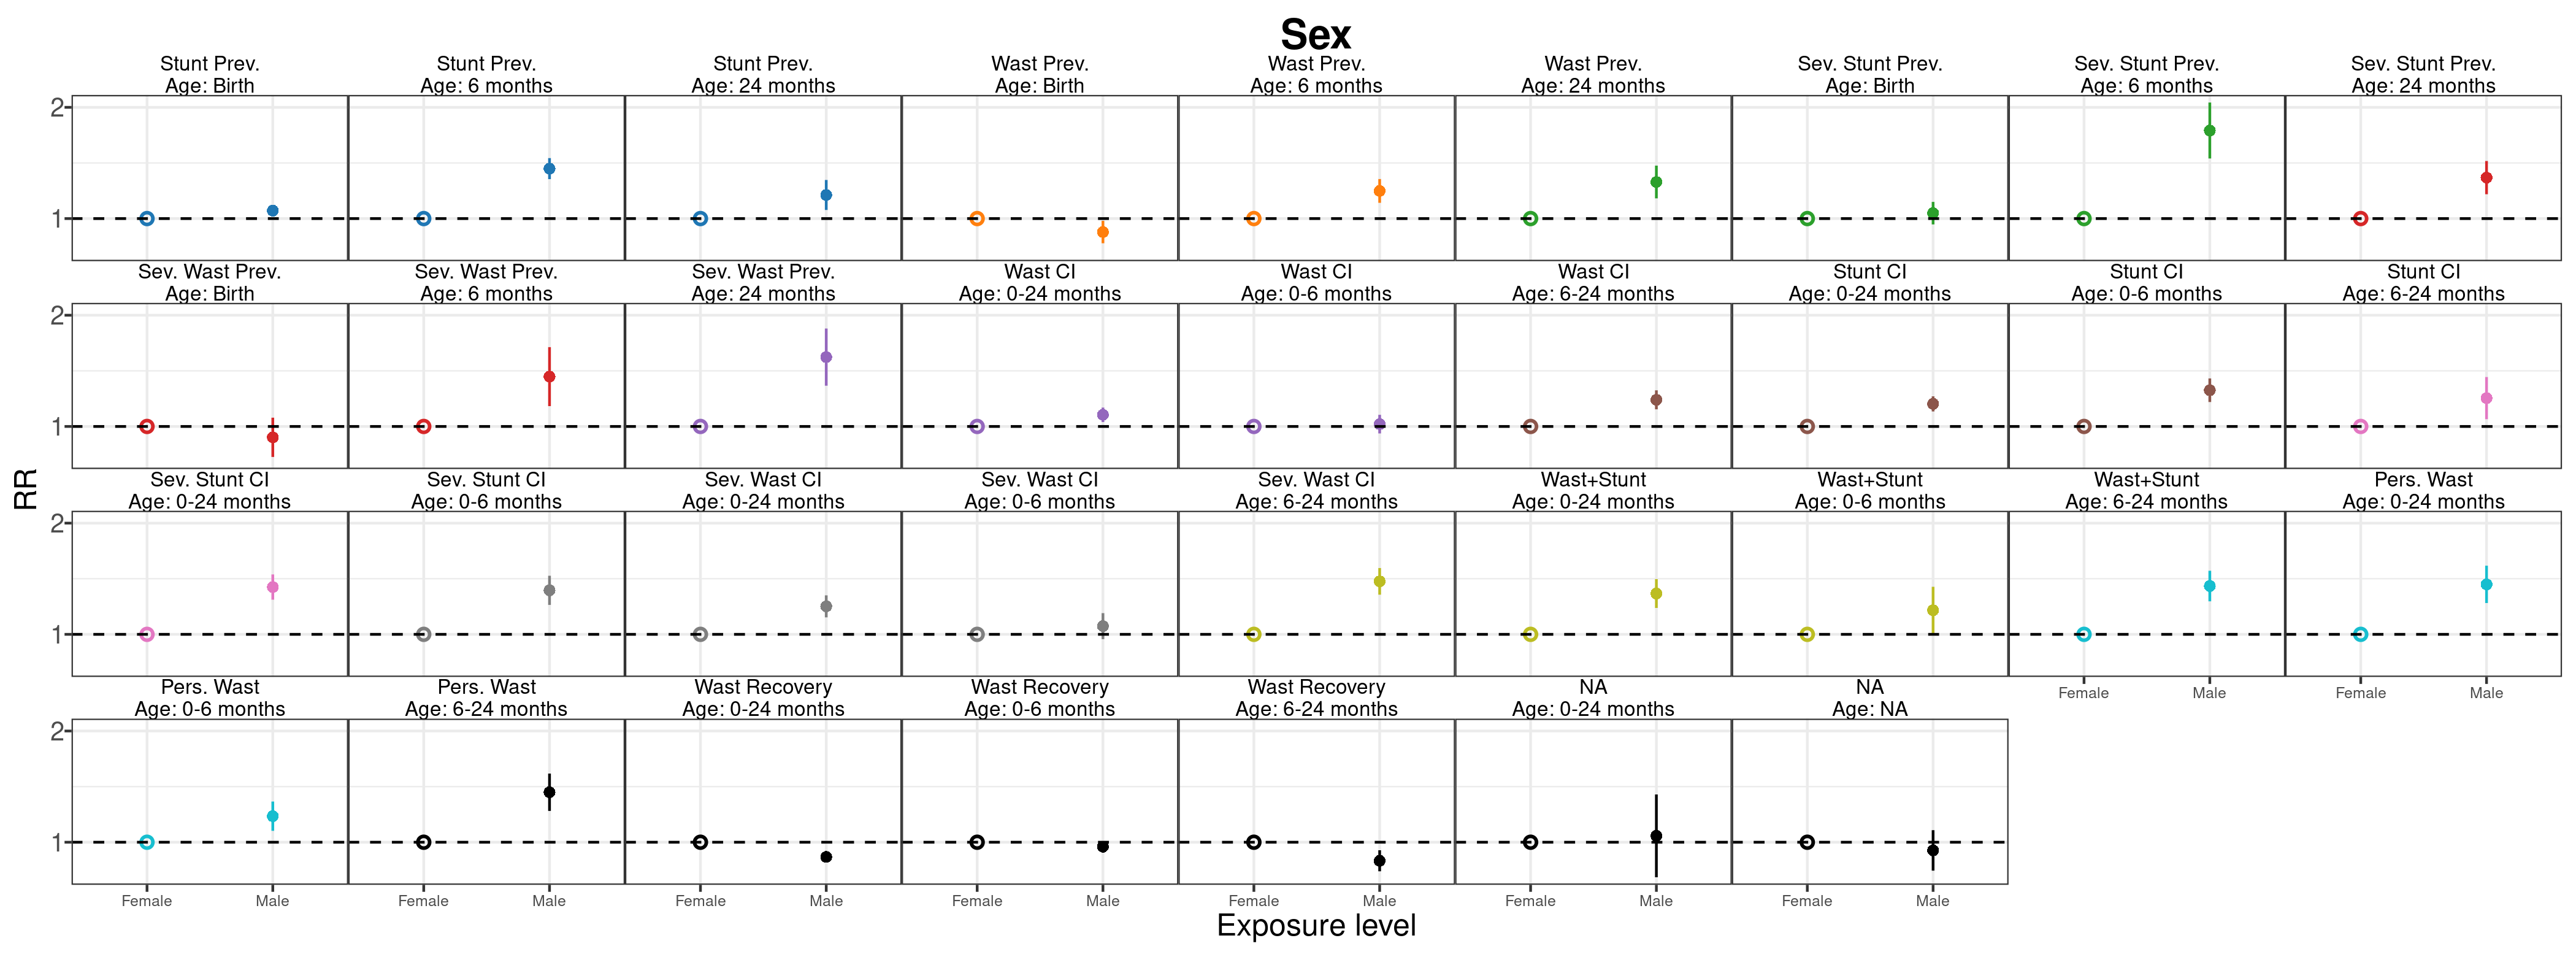
\includegraphics[width=58.33in]{C:/Users/andre/Documents/HBGDki/causes/ki-longitudinal-manuscripts/figures/risk-factor/RR-plots/fig-RR-sex}
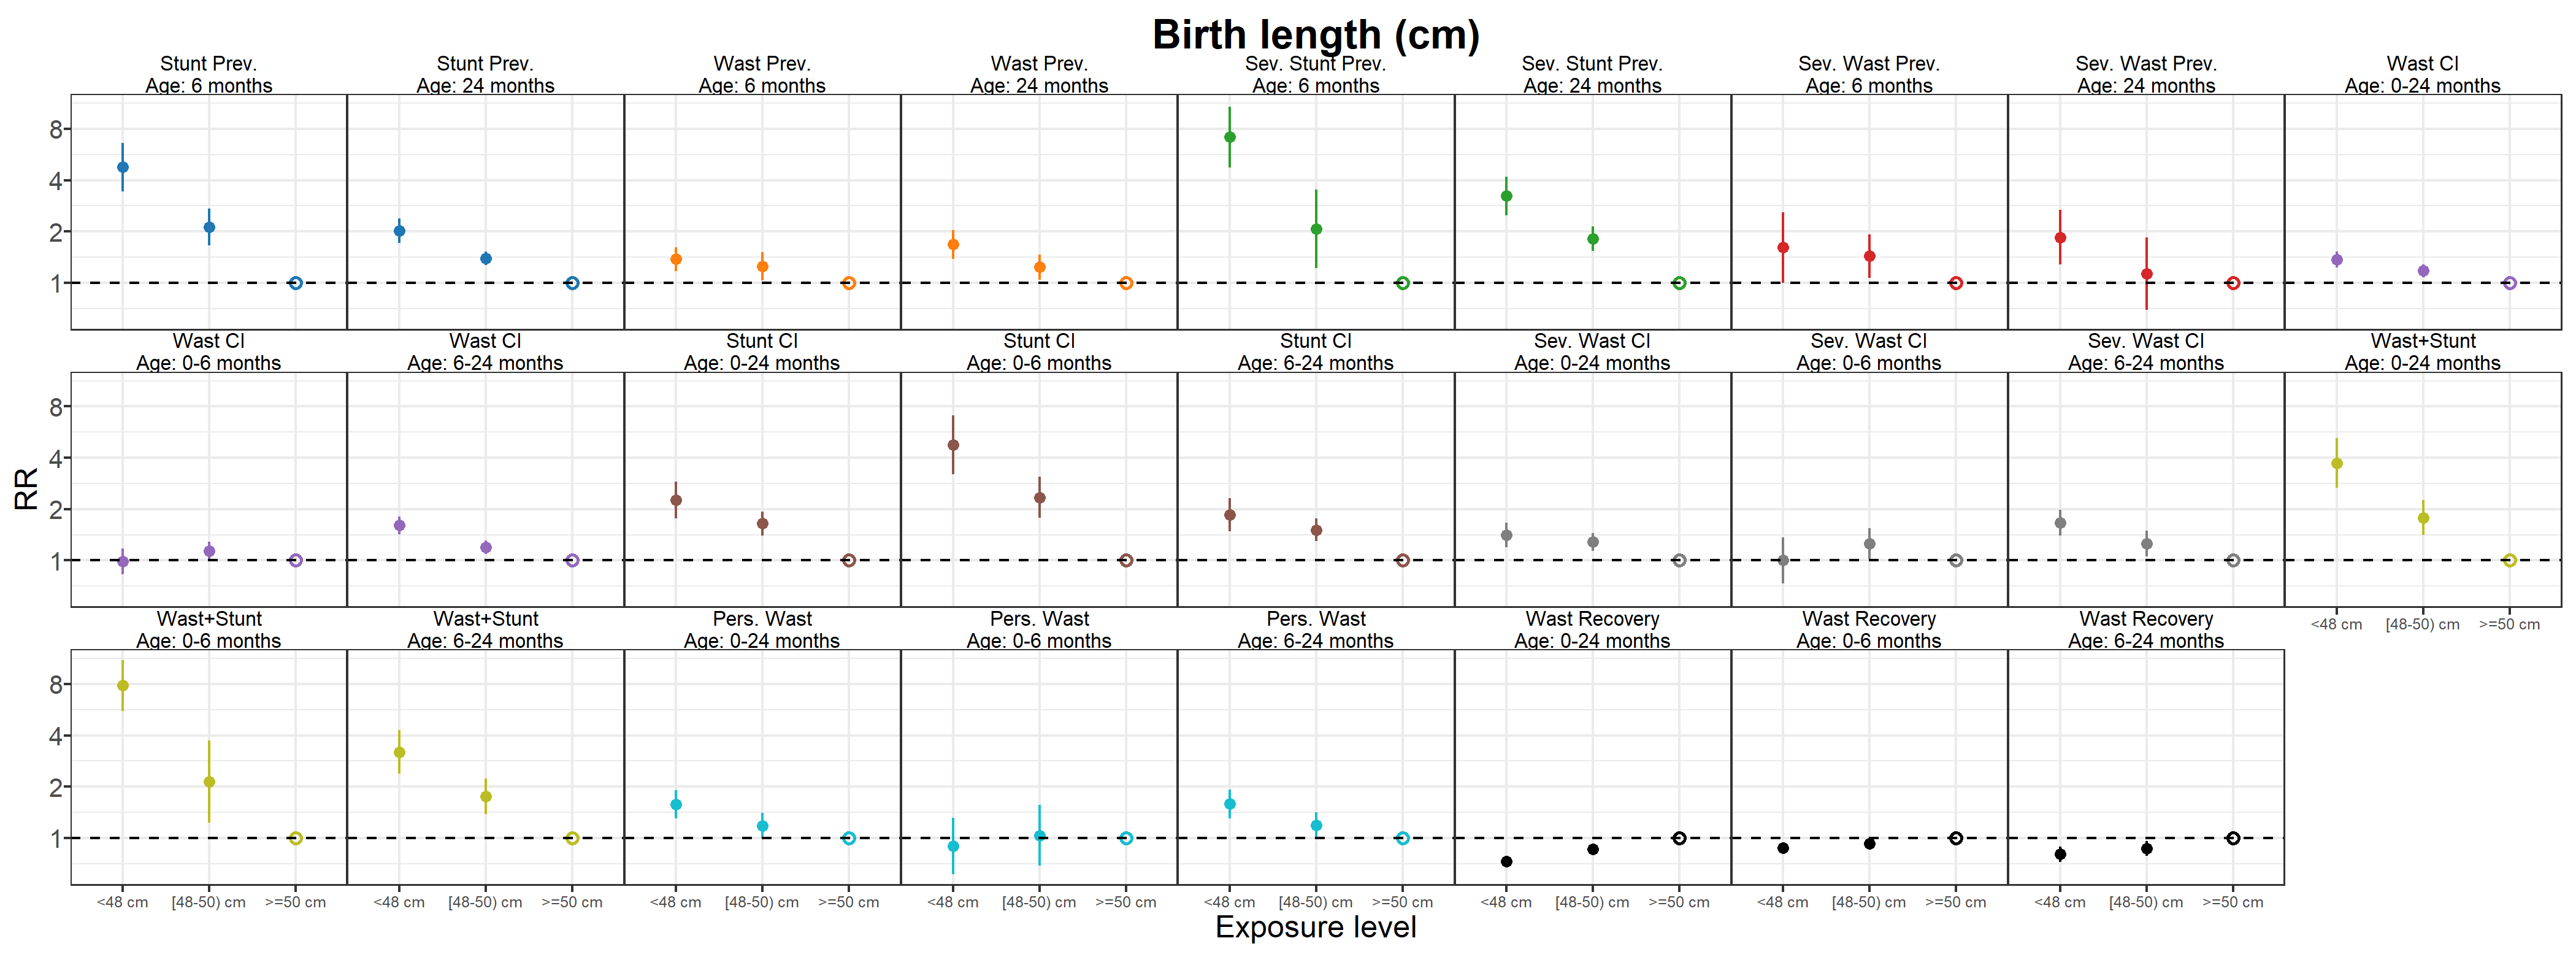
\includegraphics[width=58.33in]{C:/Users/andre/Documents/HBGDki/causes/ki-longitudinal-manuscripts/figures/risk-factor/RR-plots/fig-RR-birthlen}
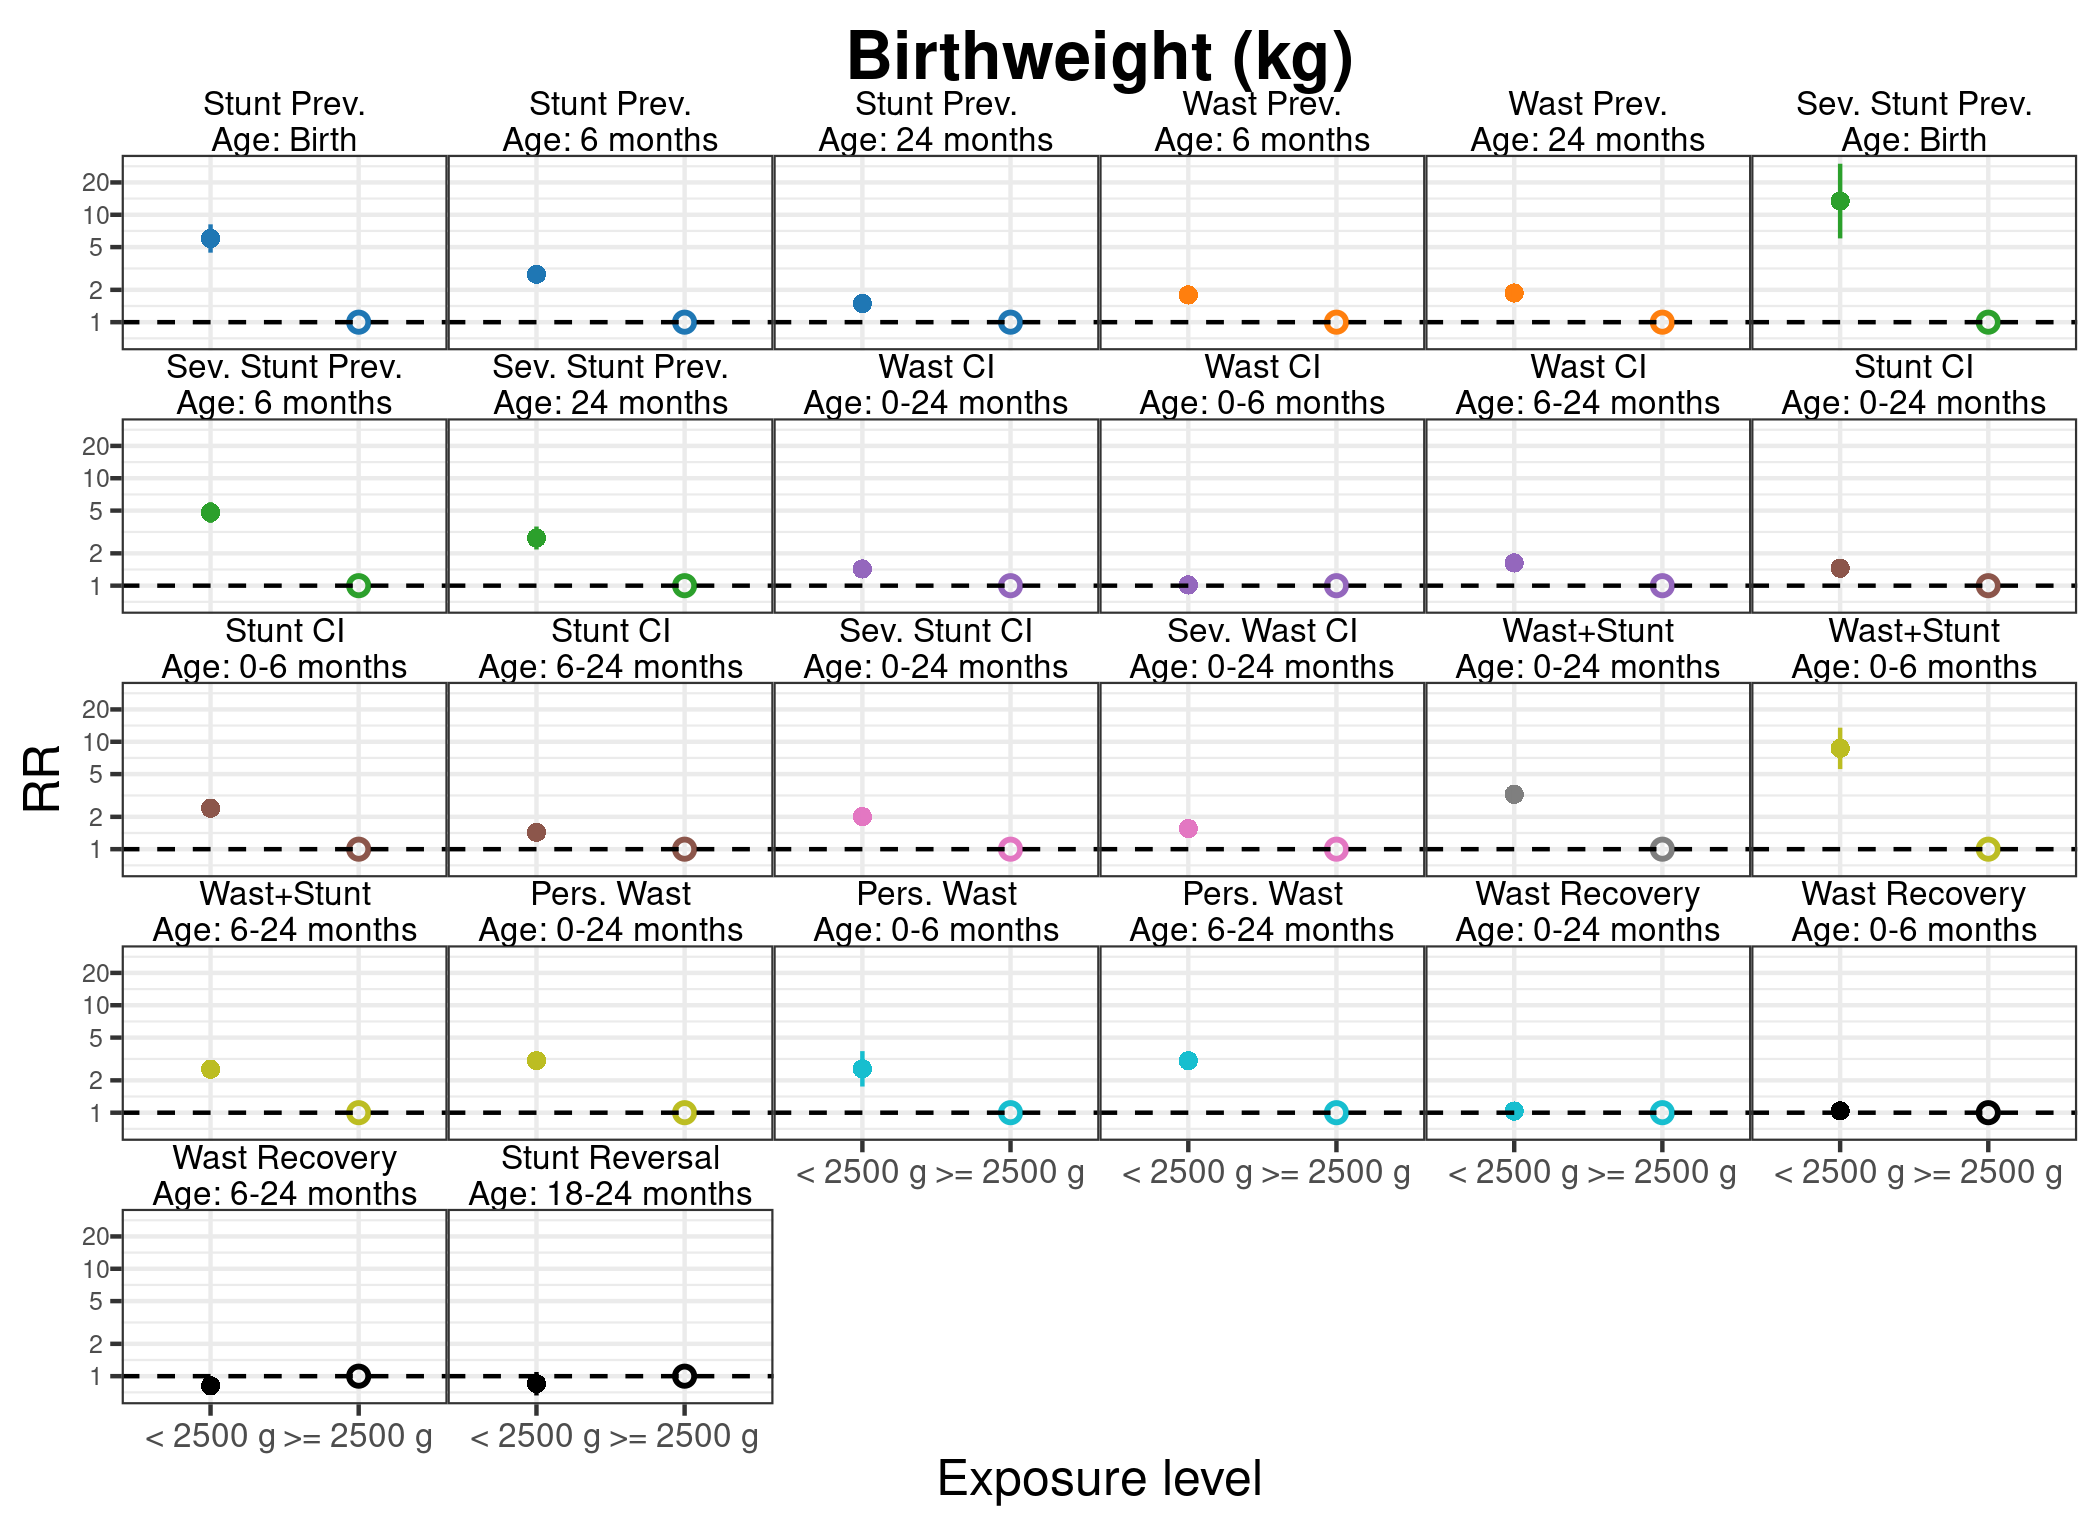
\includegraphics[width=58.33in]{C:/Users/andre/Documents/HBGDki/causes/ki-longitudinal-manuscripts/figures/risk-factor/RR-plots/fig-RR-birthwt}
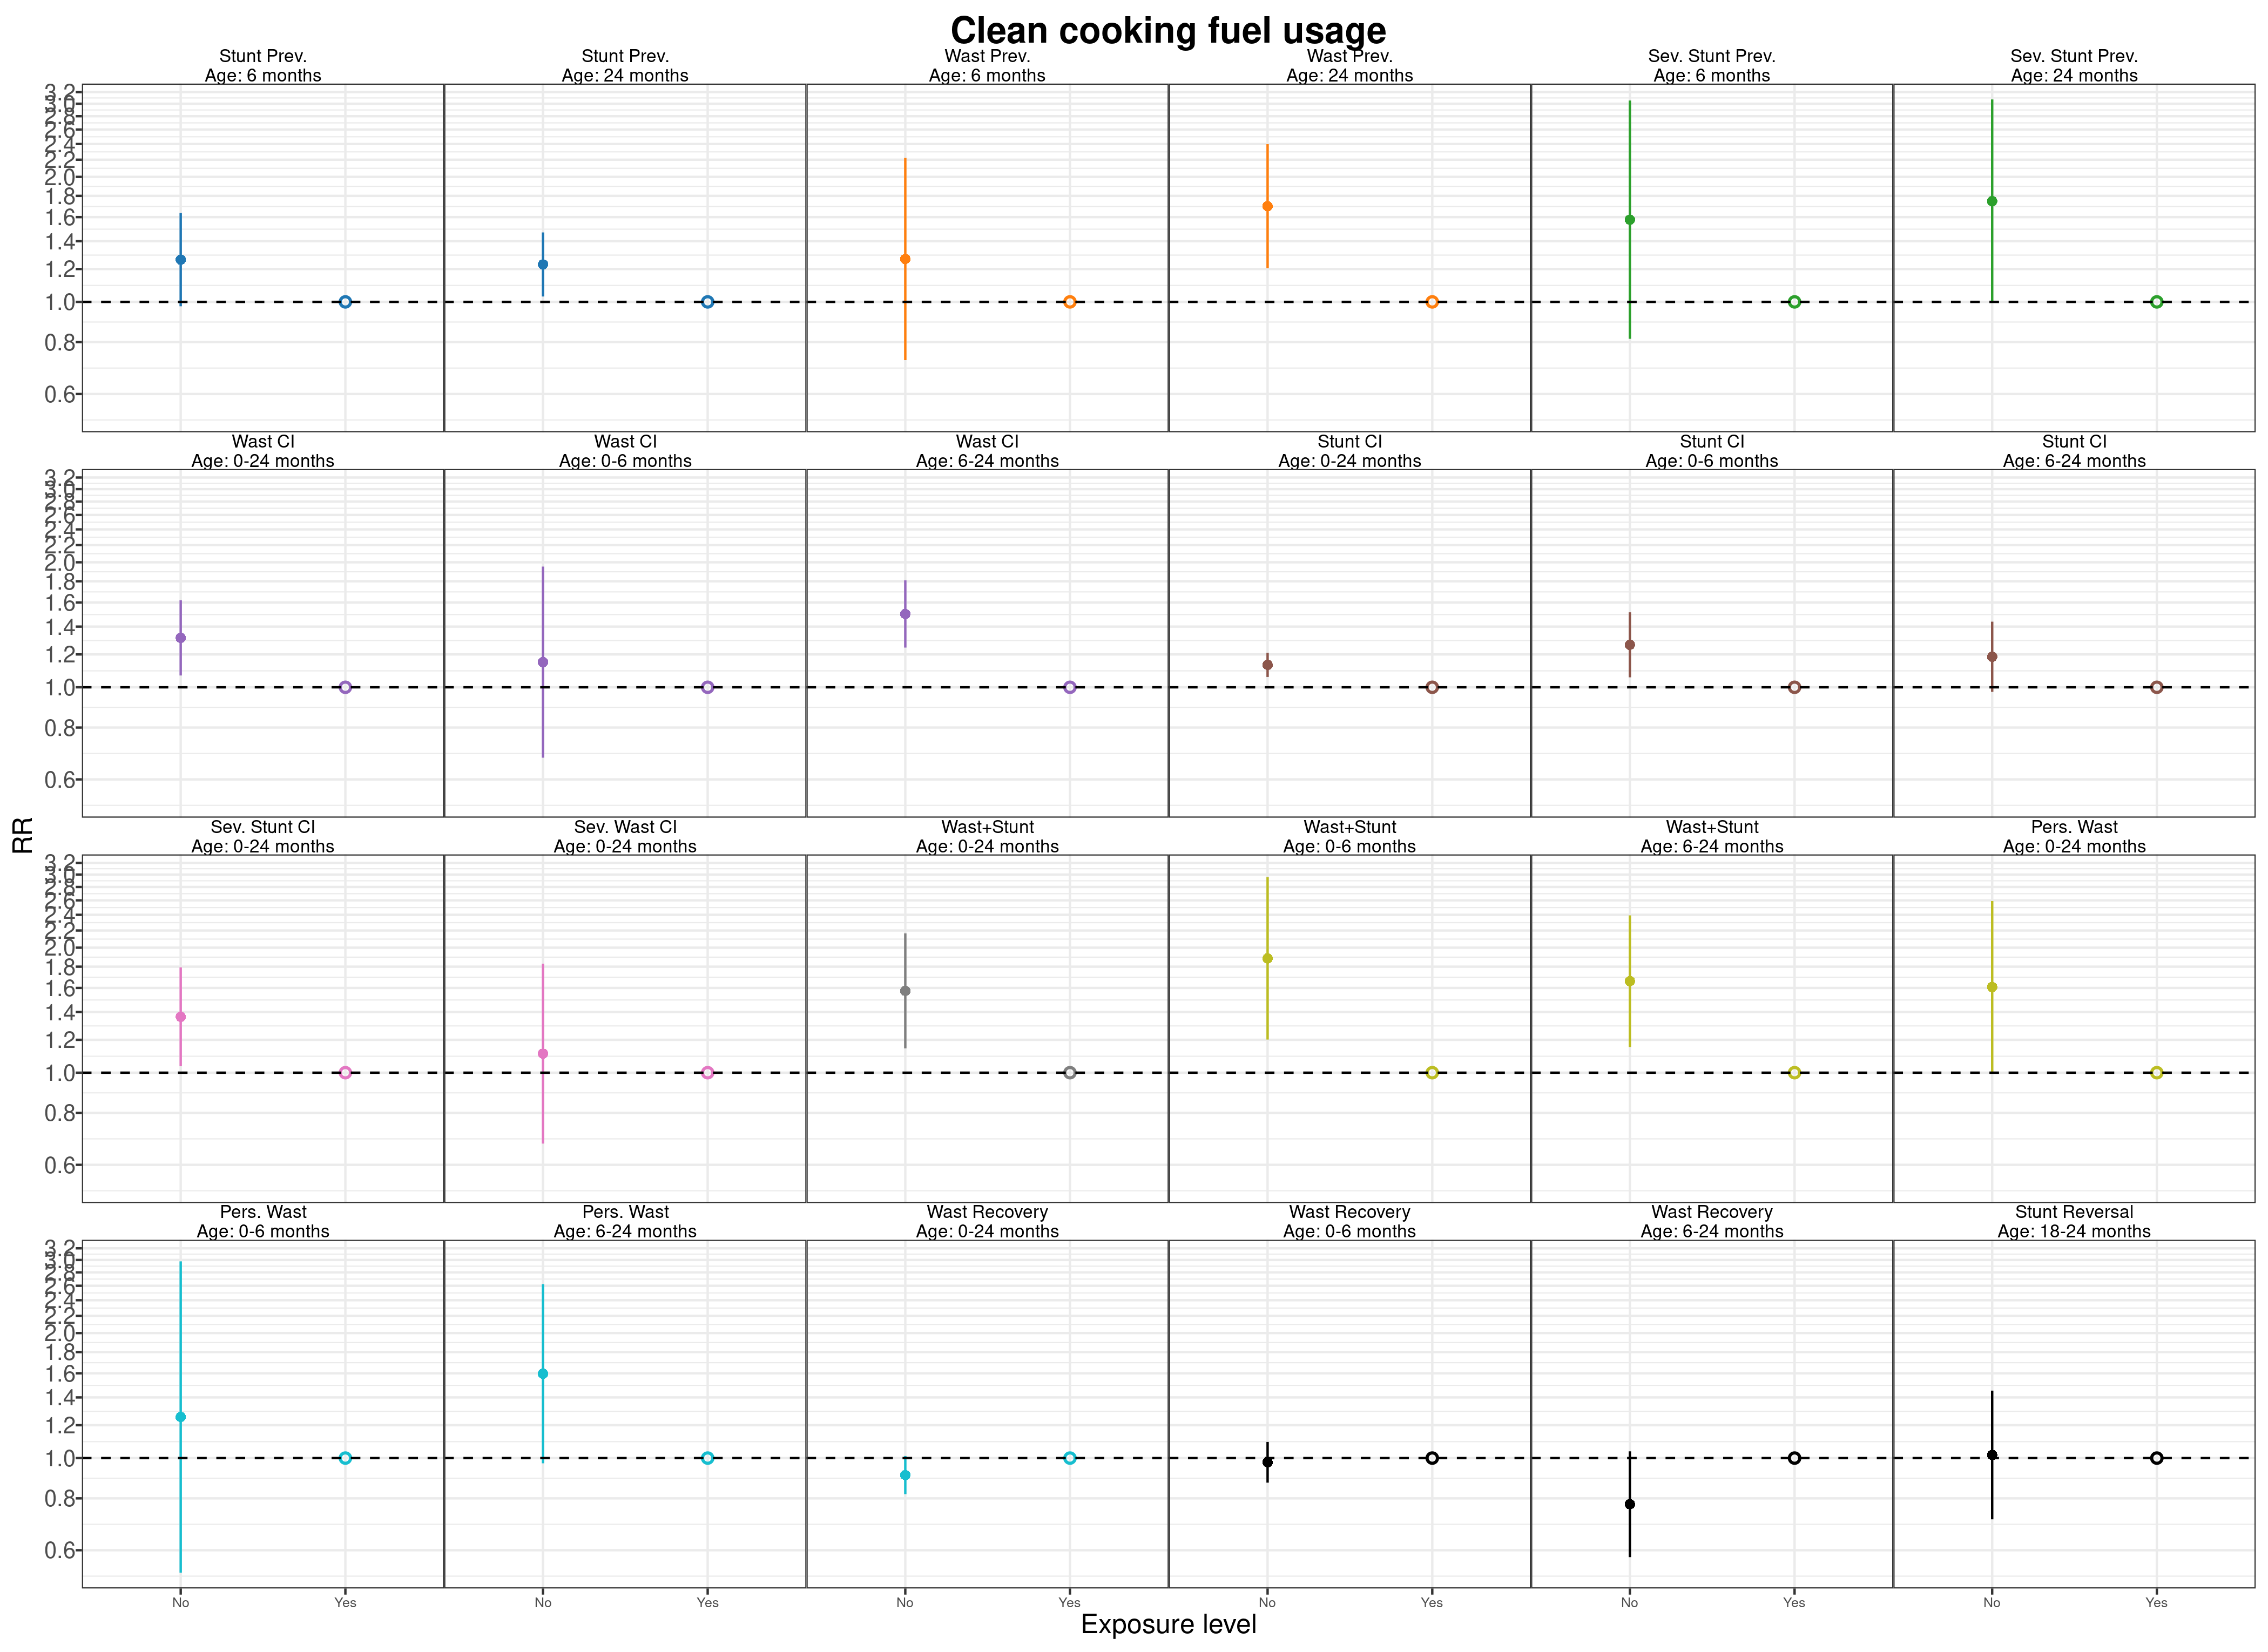
\includegraphics[width=58.33in]{C:/Users/andre/Documents/HBGDki/causes/ki-longitudinal-manuscripts/figures/risk-factor/RR-plots/fig-RR-cleanck}
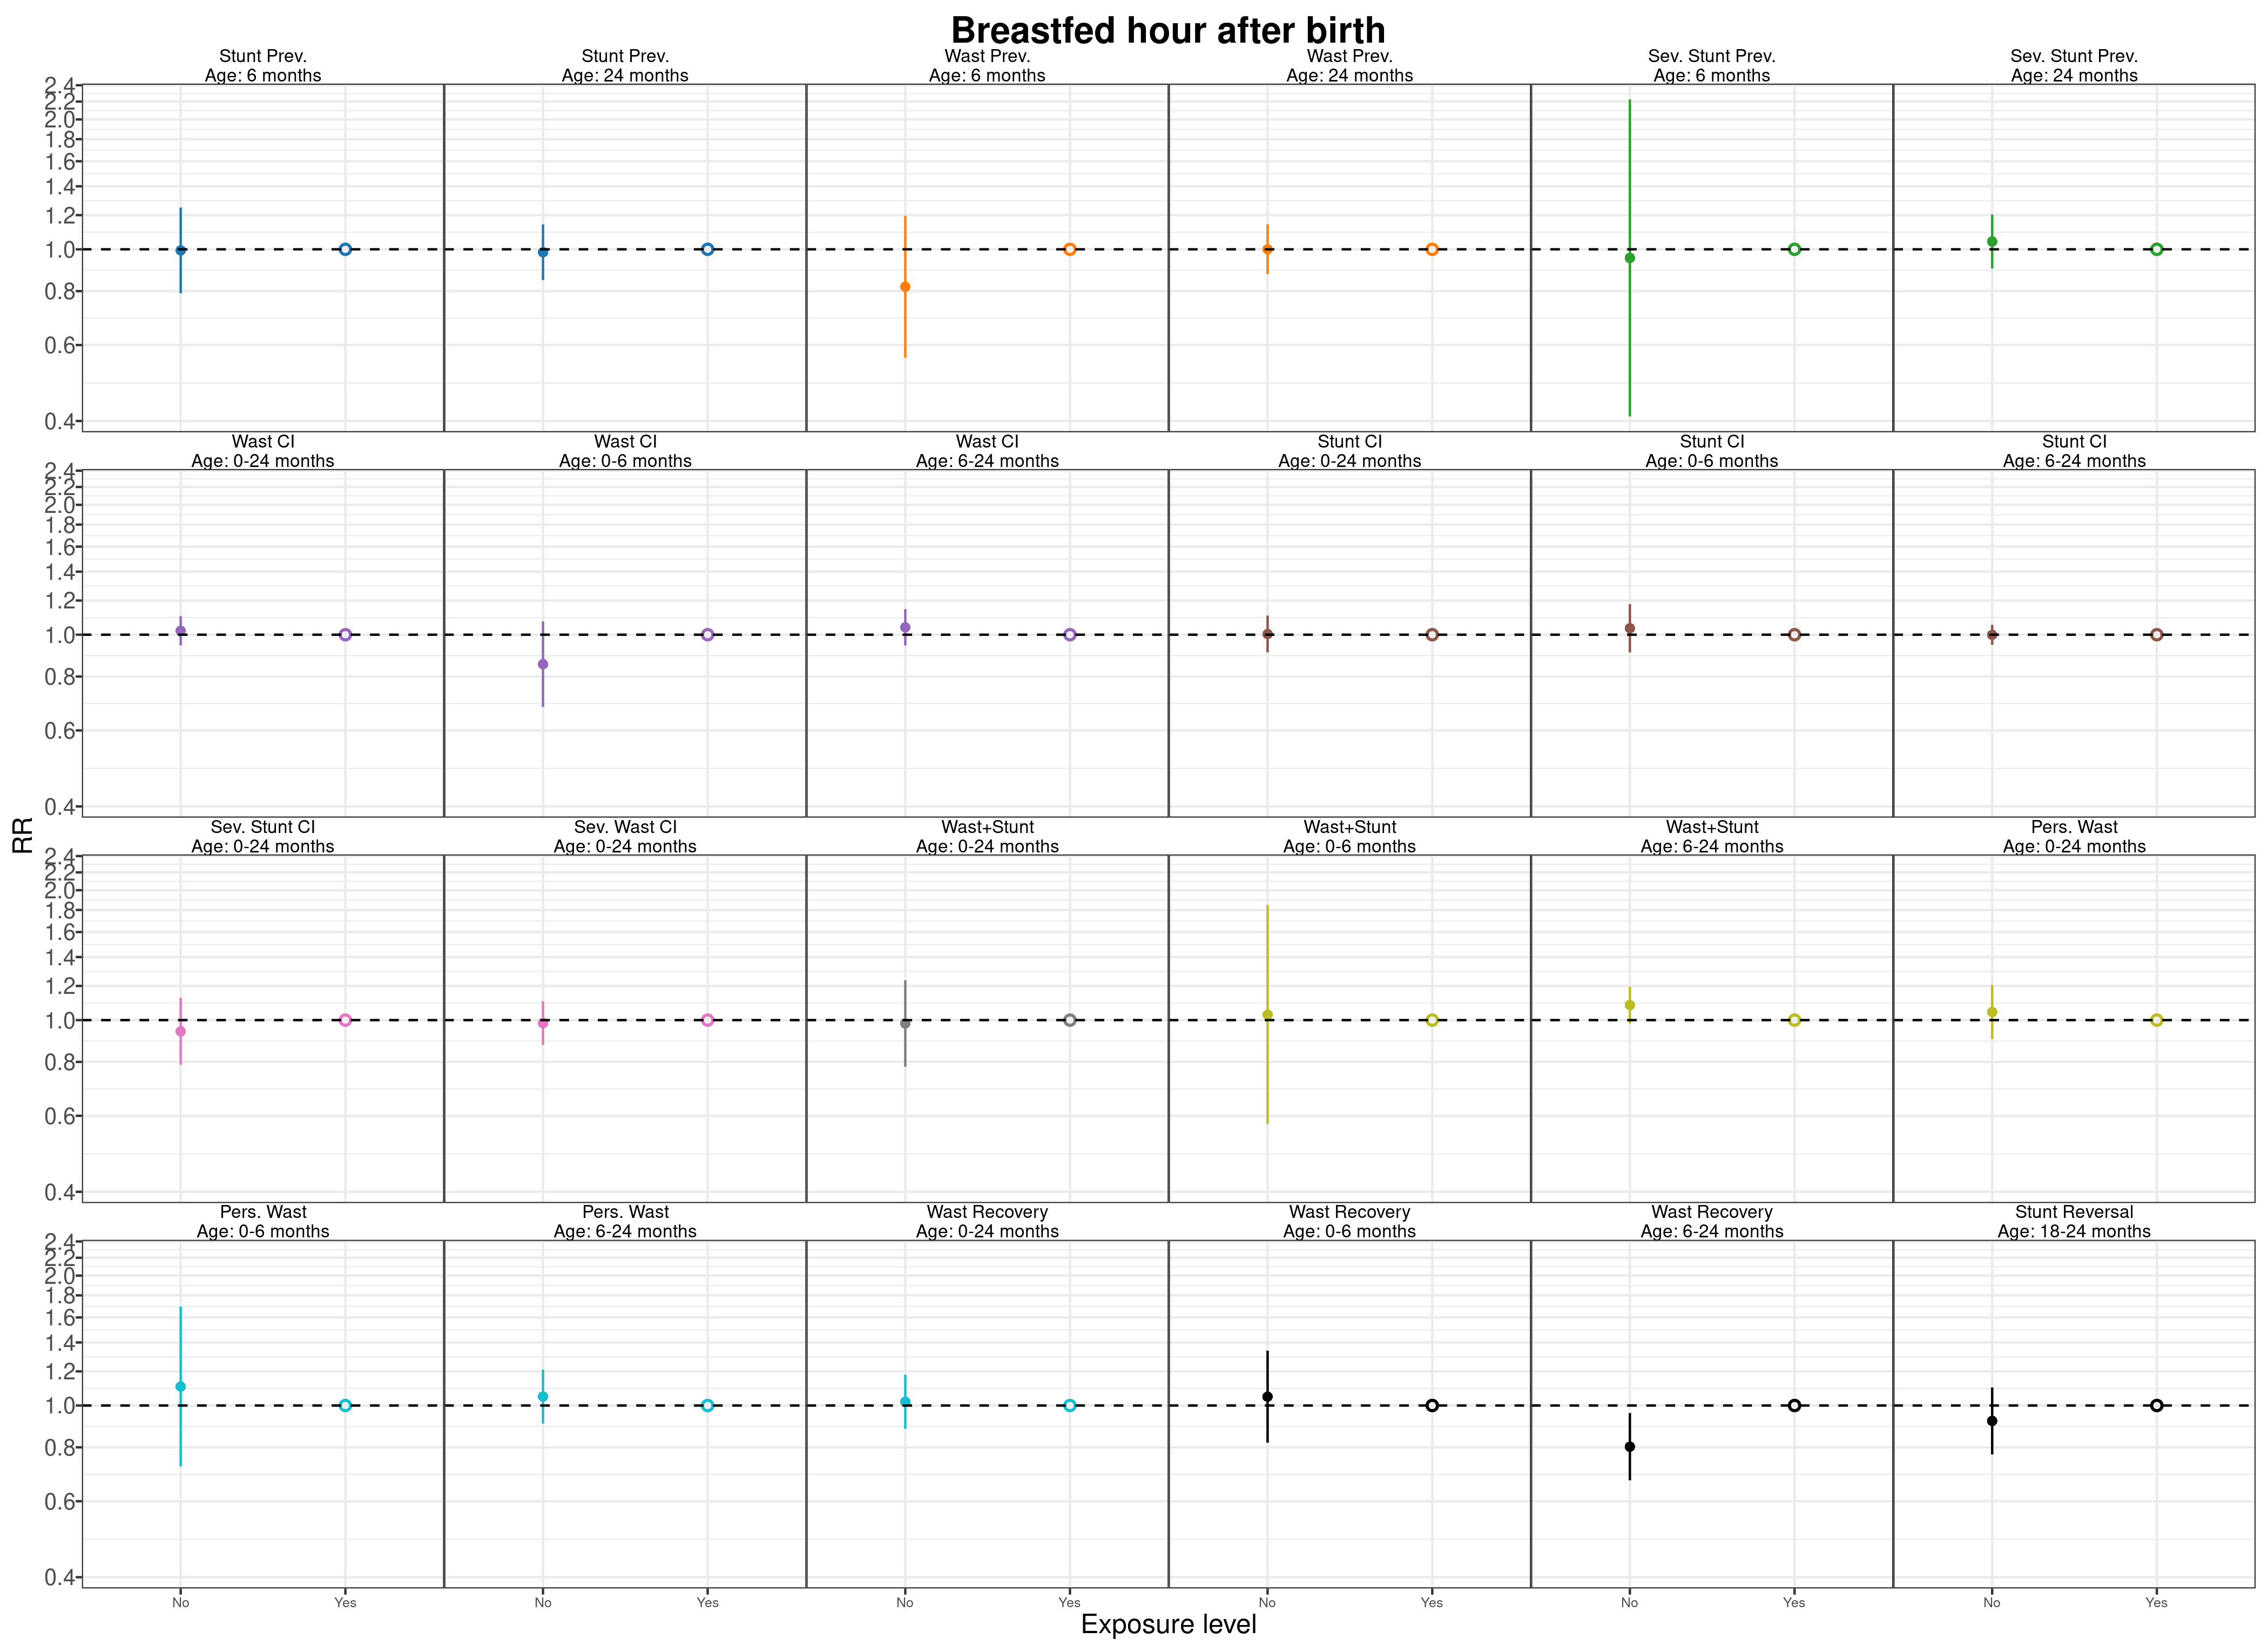
\includegraphics[width=58.33in]{C:/Users/andre/Documents/HBGDki/causes/ki-longitudinal-manuscripts/figures/risk-factor/RR-plots/fig-RR-earlybf}
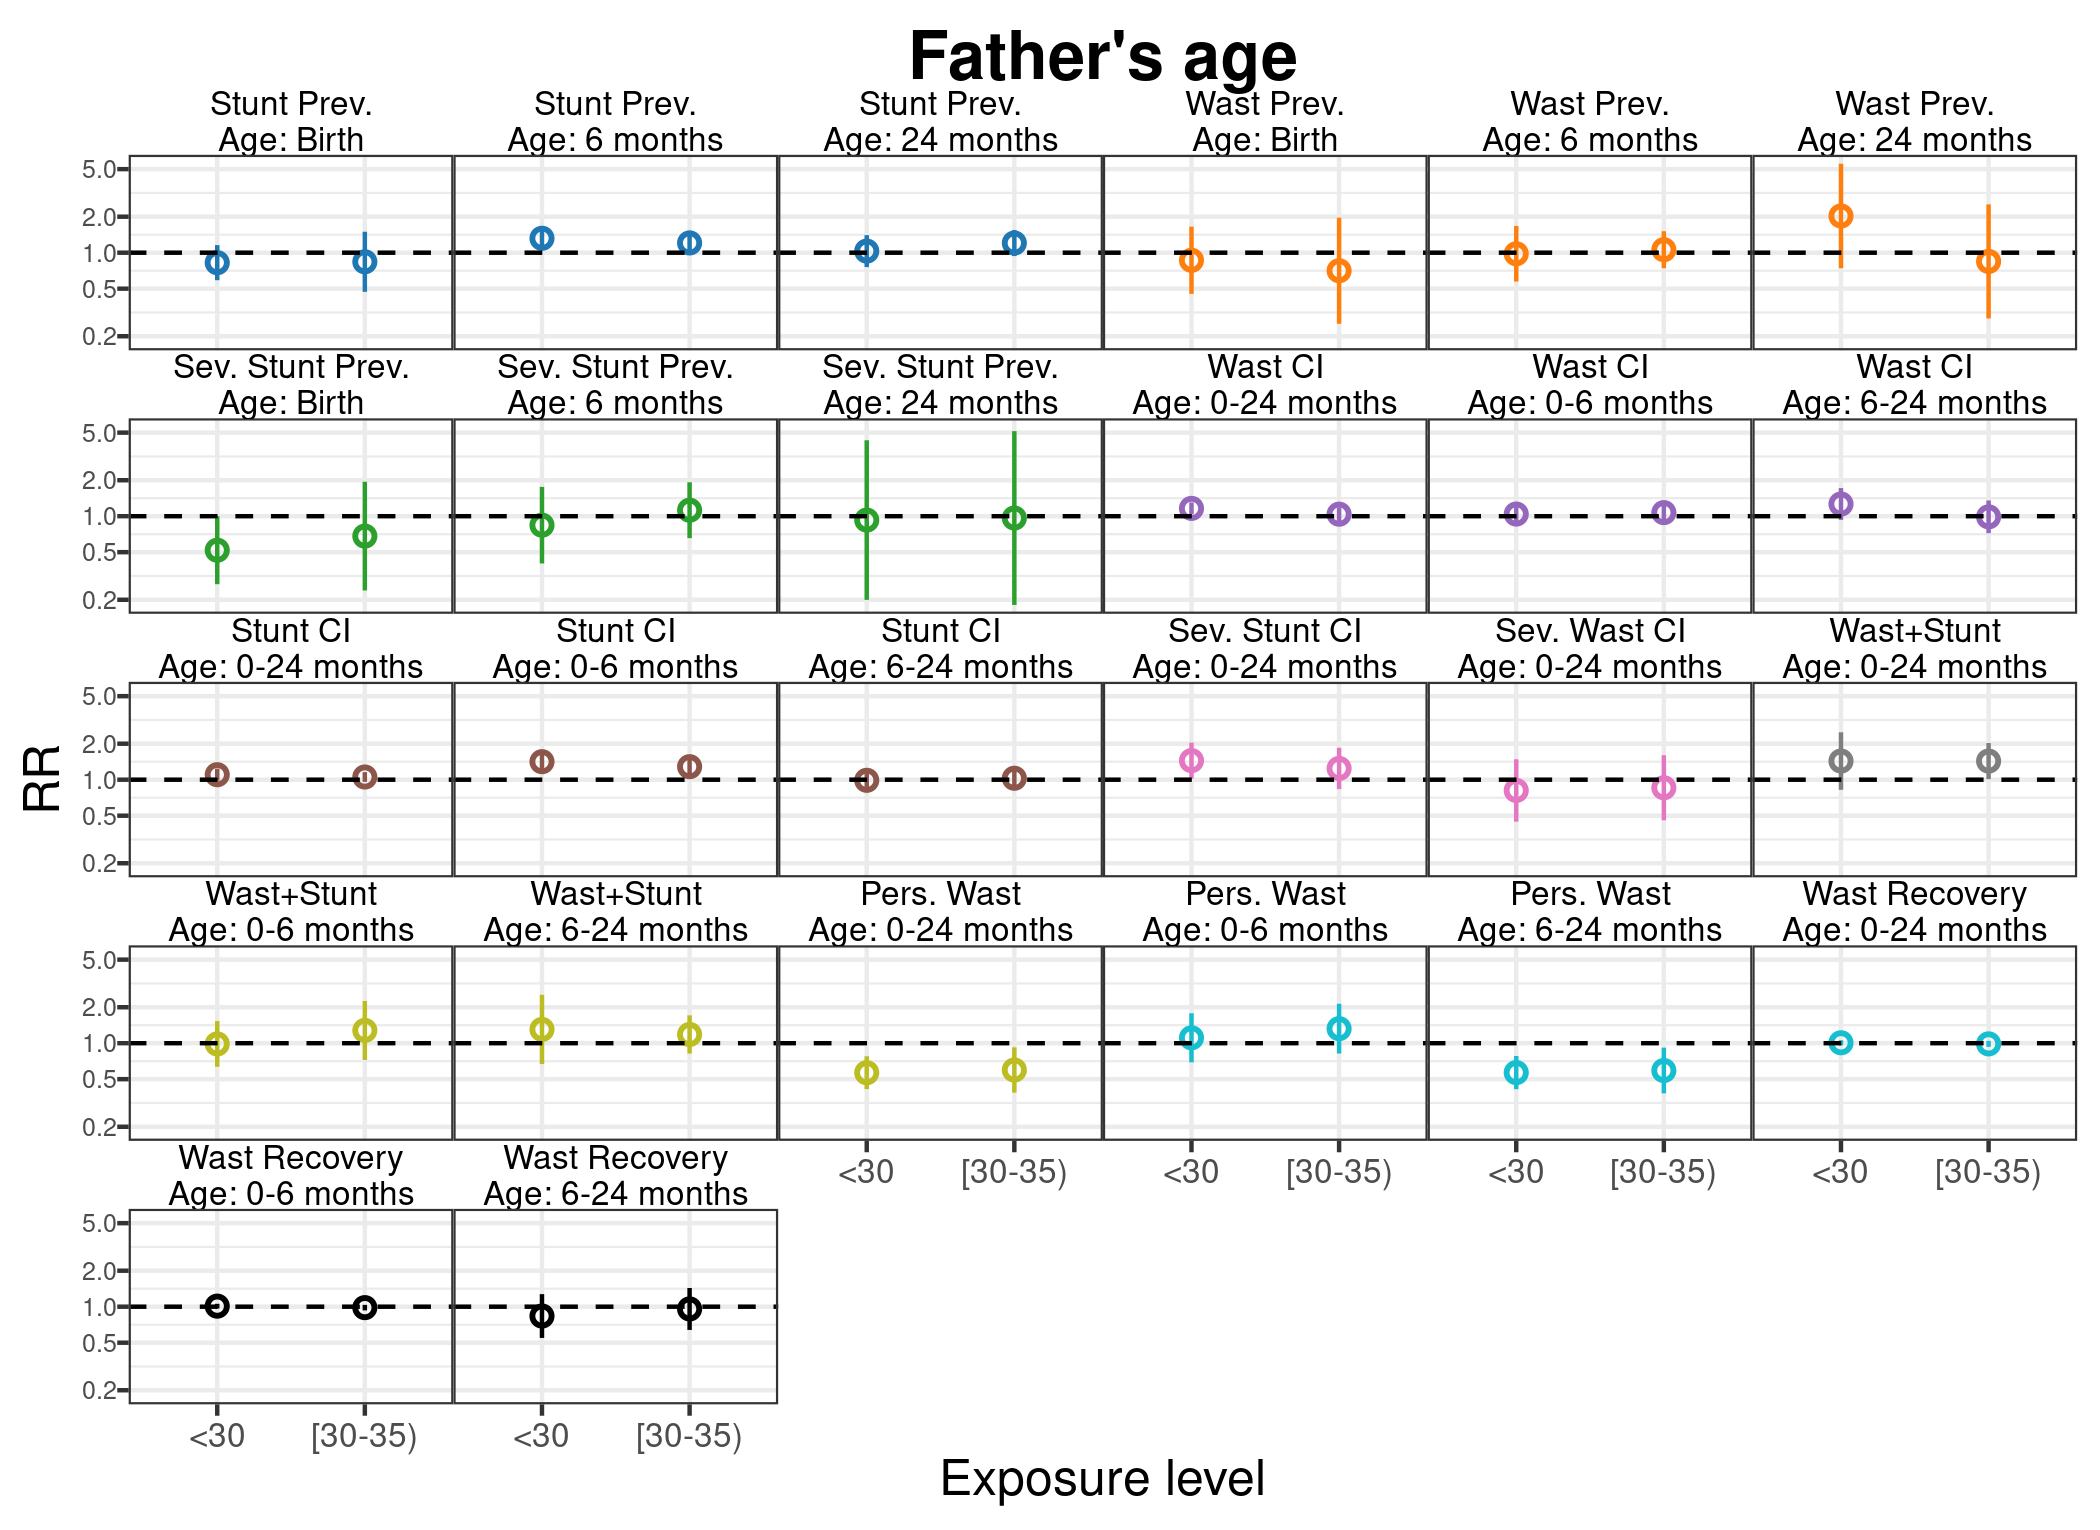
\includegraphics[width=58.33in]{C:/Users/andre/Documents/HBGDki/causes/ki-longitudinal-manuscripts/figures/risk-factor/RR-plots/fig-RR-fage}
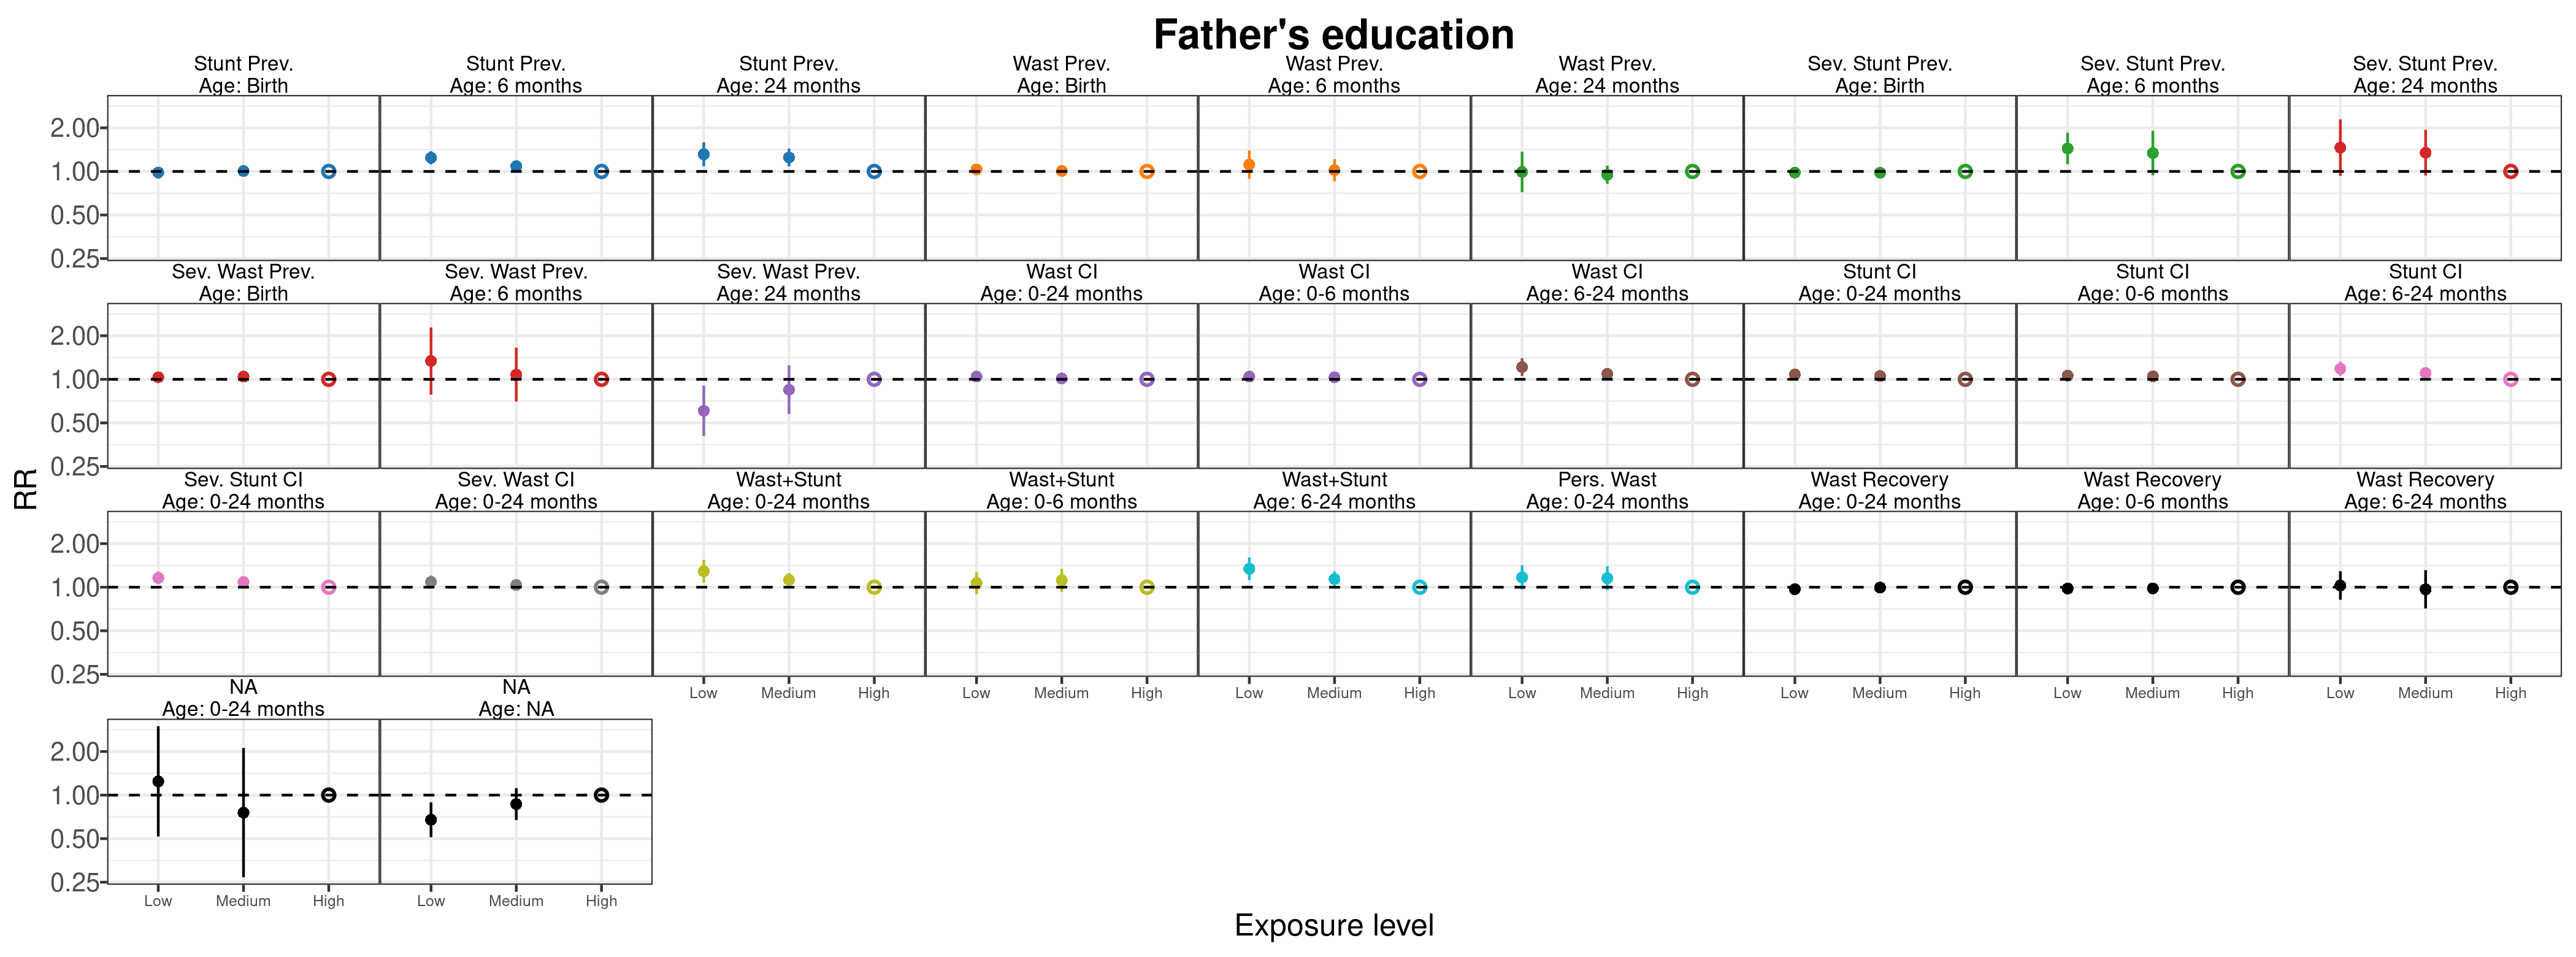
\includegraphics[width=58.33in]{C:/Users/andre/Documents/HBGDki/causes/ki-longitudinal-manuscripts/figures/risk-factor/RR-plots/fig-RR-feducyrs}
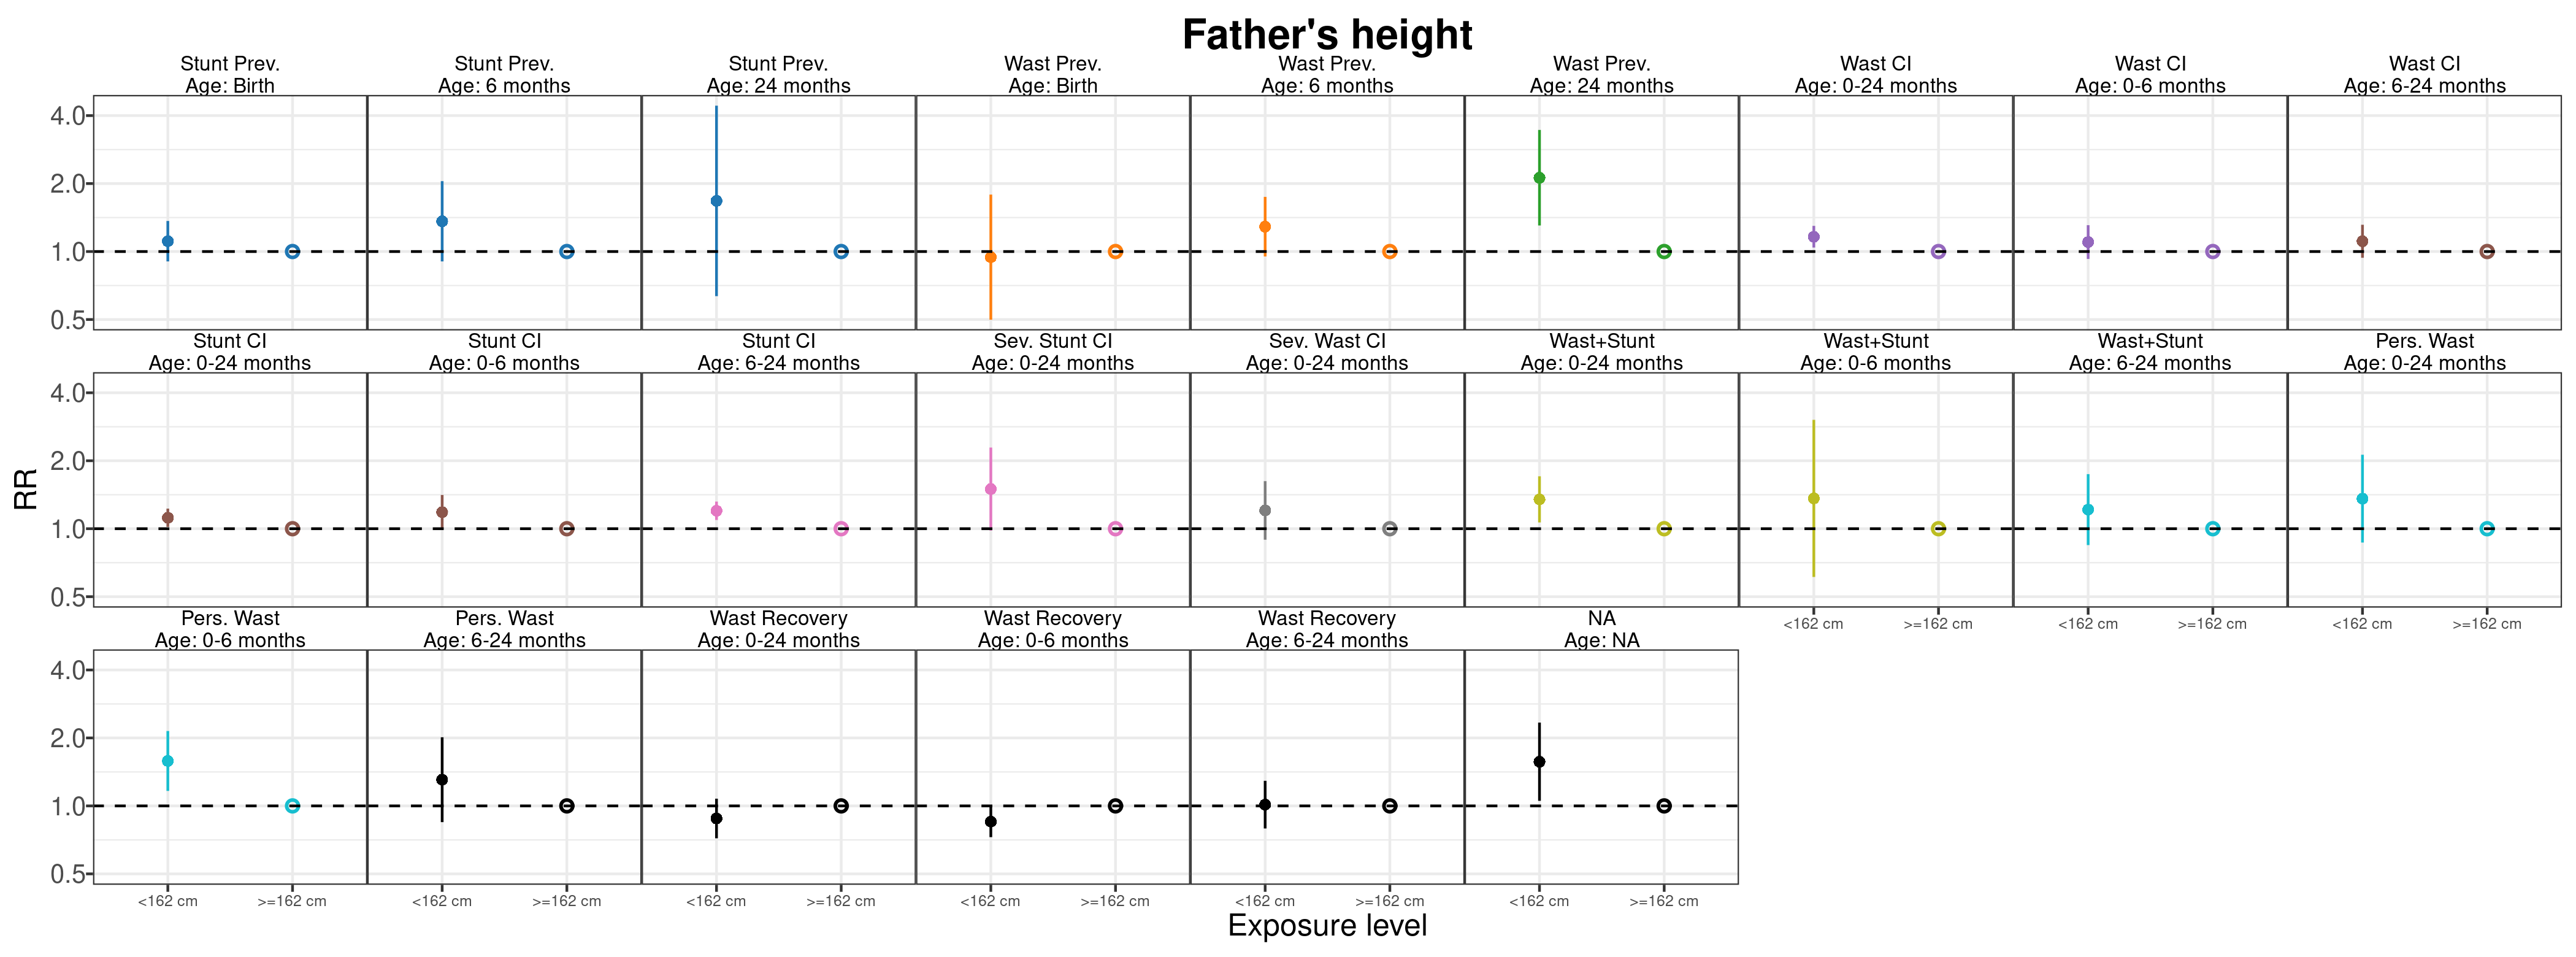
\includegraphics[width=58.33in]{C:/Users/andre/Documents/HBGDki/causes/ki-longitudinal-manuscripts/figures/risk-factor/RR-plots/fig-RR-fhtcm}
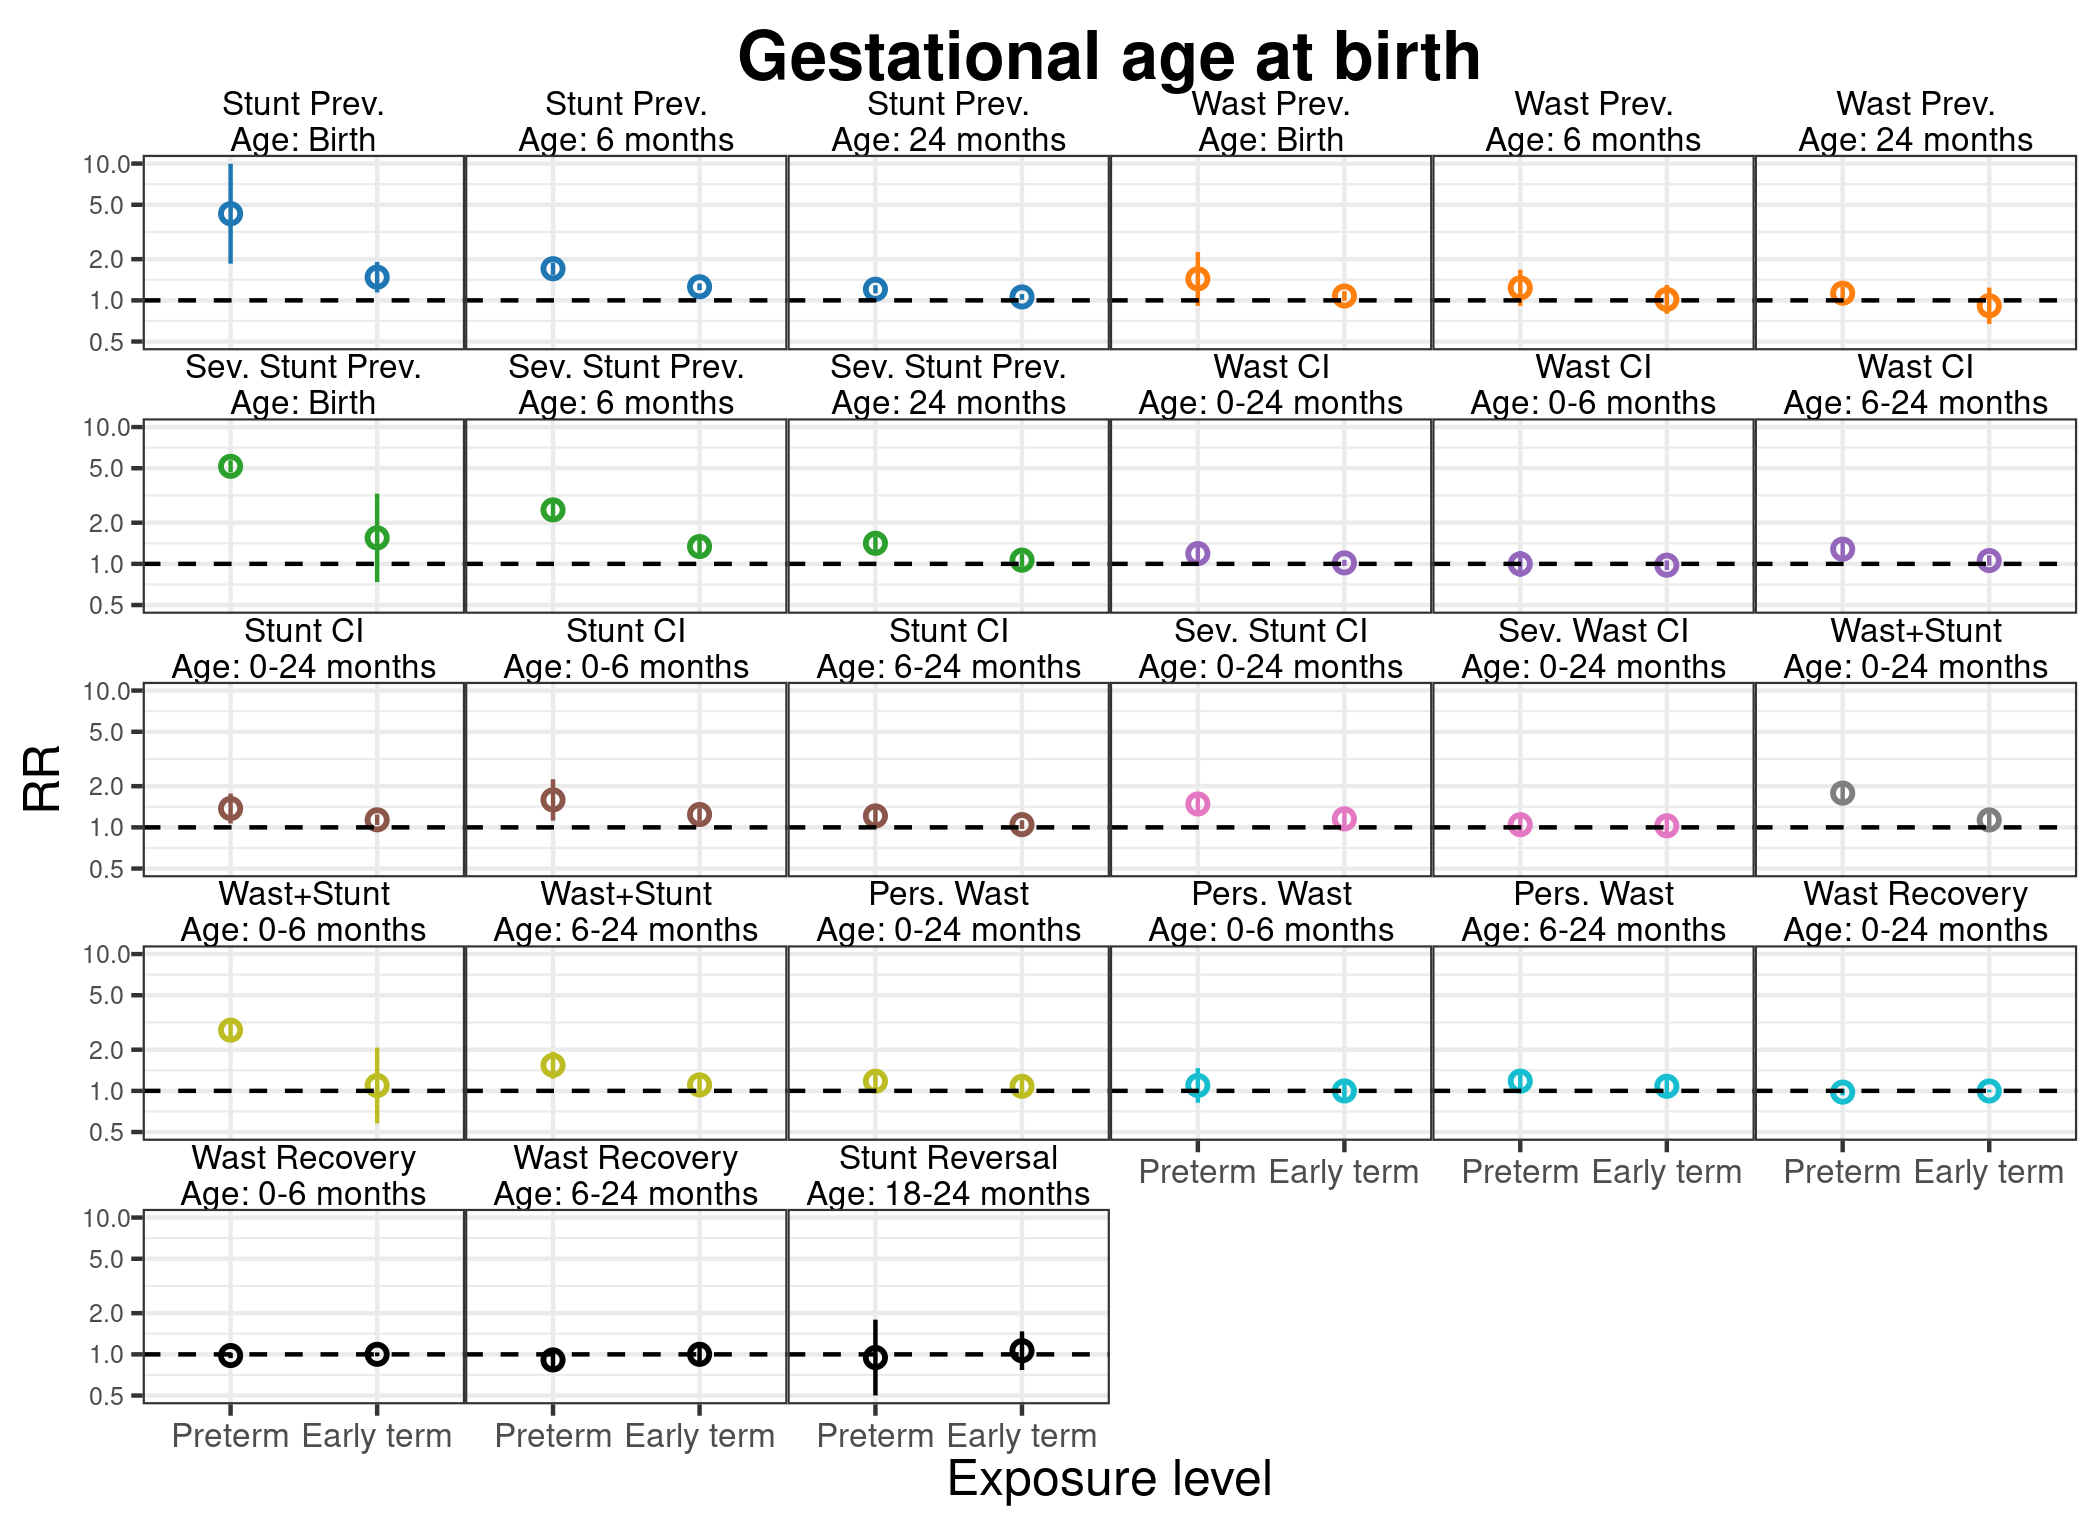
\includegraphics[width=58.33in]{C:/Users/andre/Documents/HBGDki/causes/ki-longitudinal-manuscripts/figures/risk-factor/RR-plots/fig-RR-gagebrth}
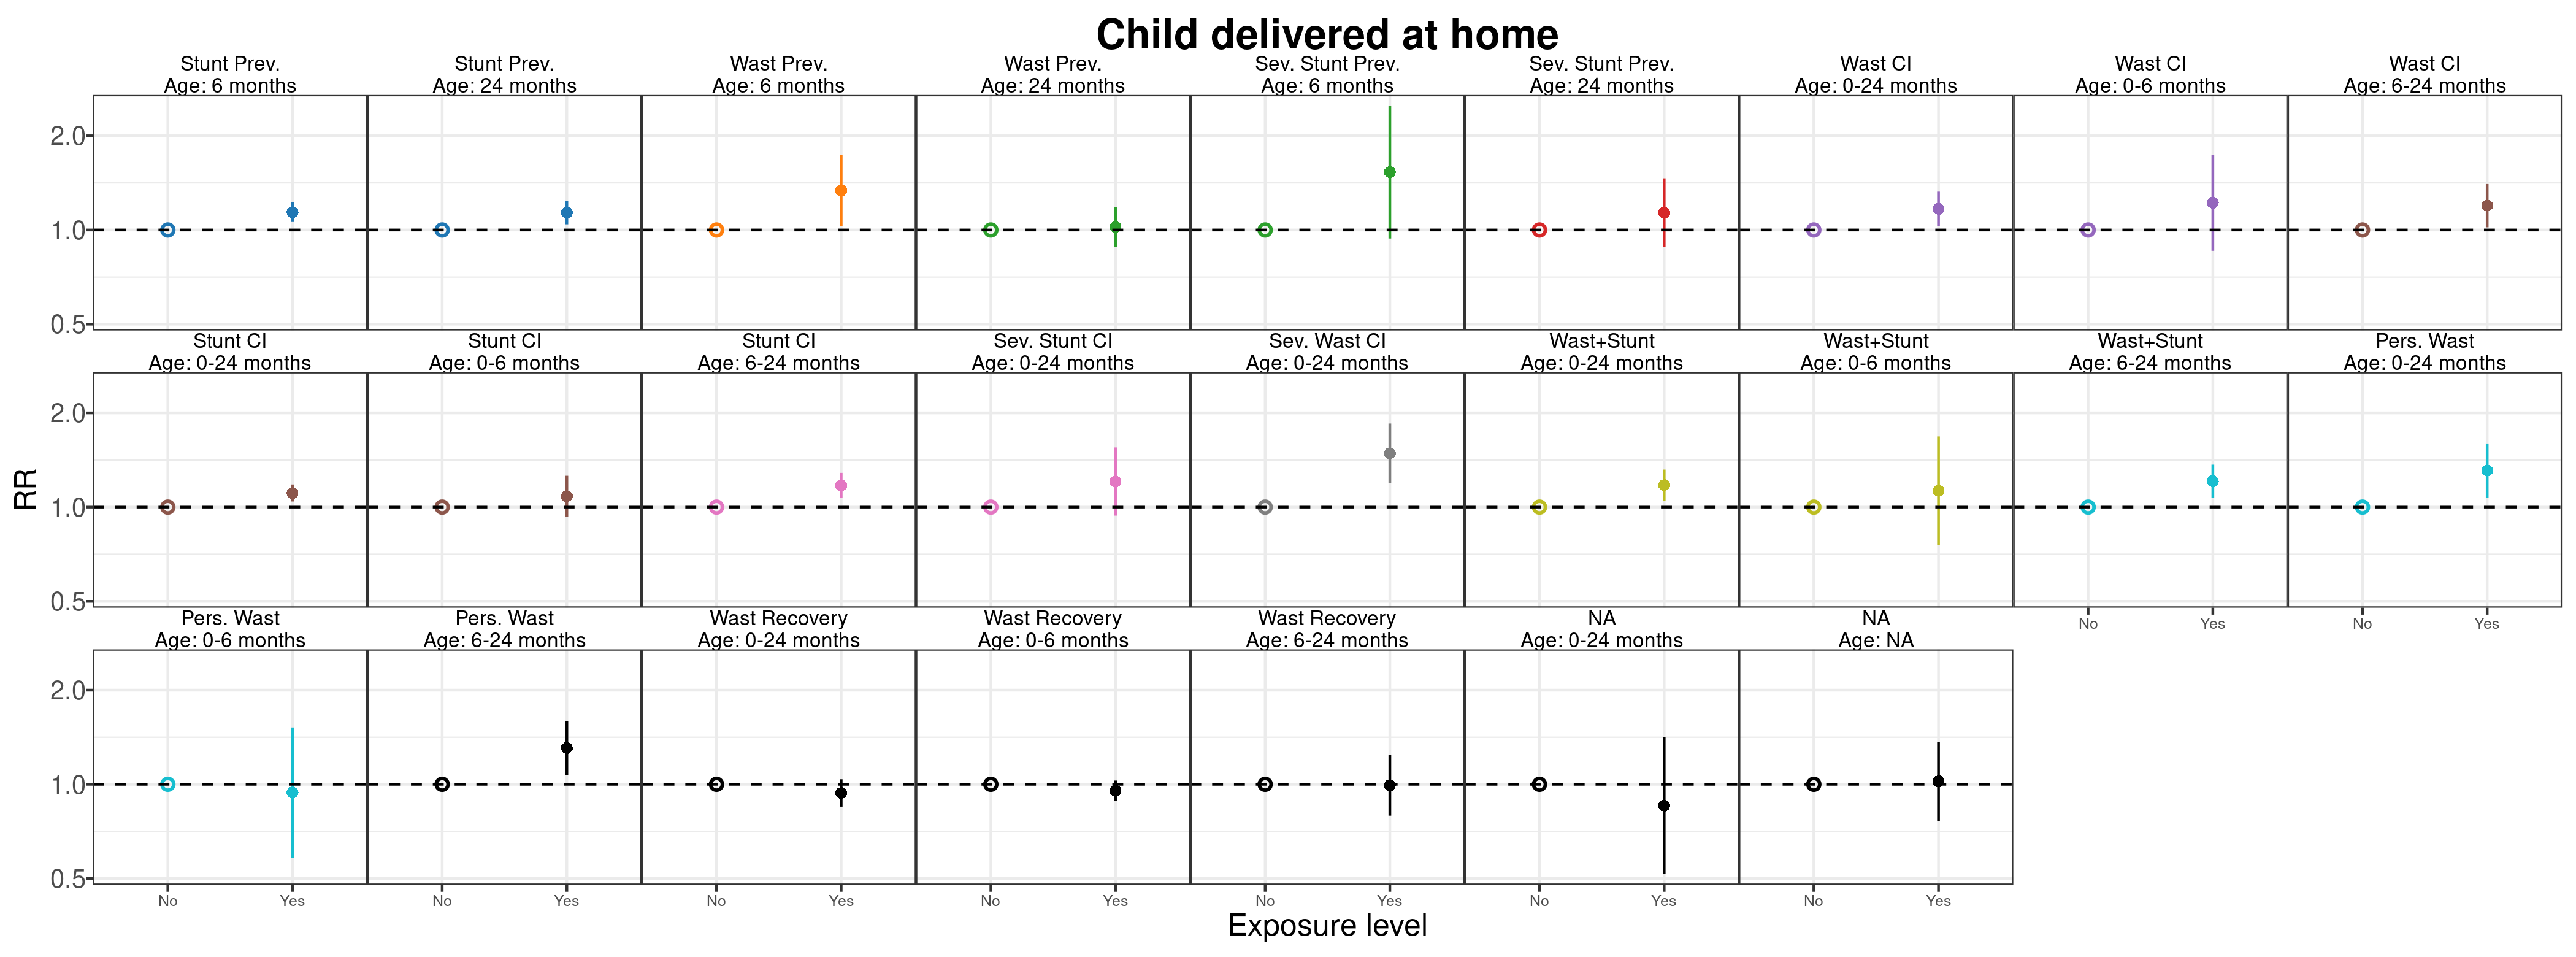
\includegraphics[width=58.33in]{C:/Users/andre/Documents/HBGDki/causes/ki-longitudinal-manuscripts/figures/risk-factor/RR-plots/fig-RR-hdlvry}
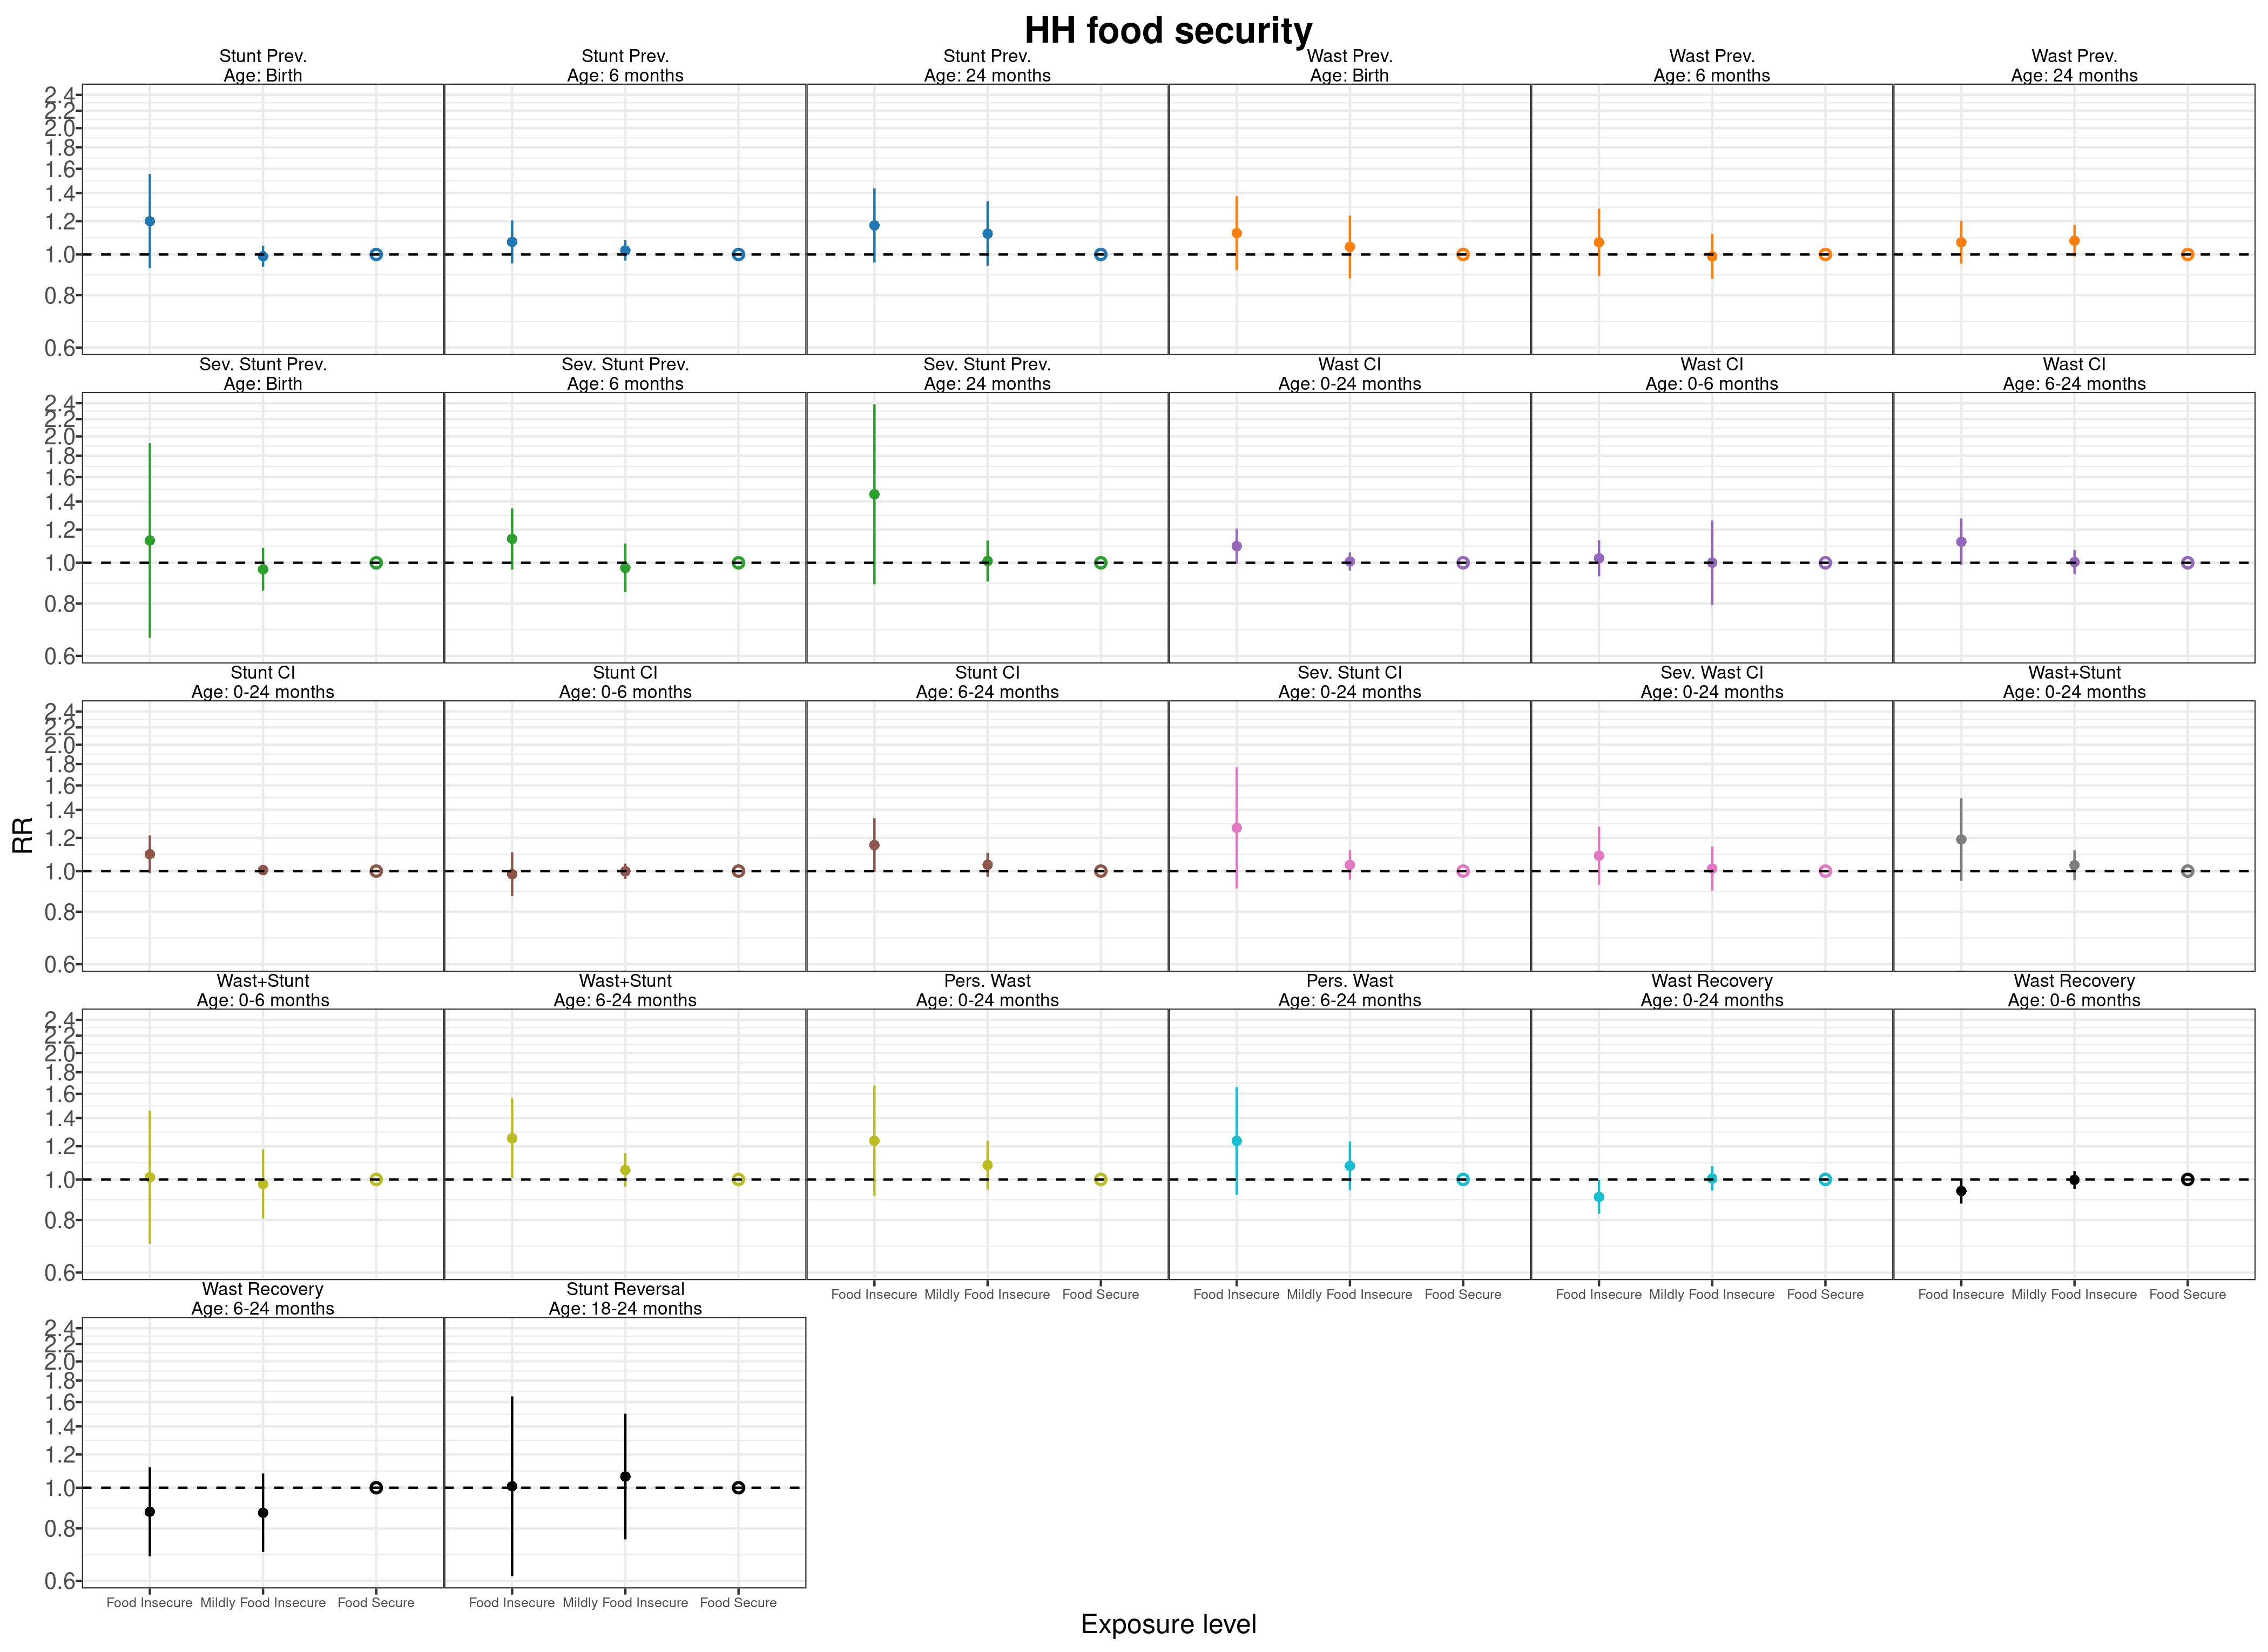
\includegraphics[width=58.33in]{C:/Users/andre/Documents/HBGDki/causes/ki-longitudinal-manuscripts/figures/risk-factor/RR-plots/fig-RR-hfoodsec}
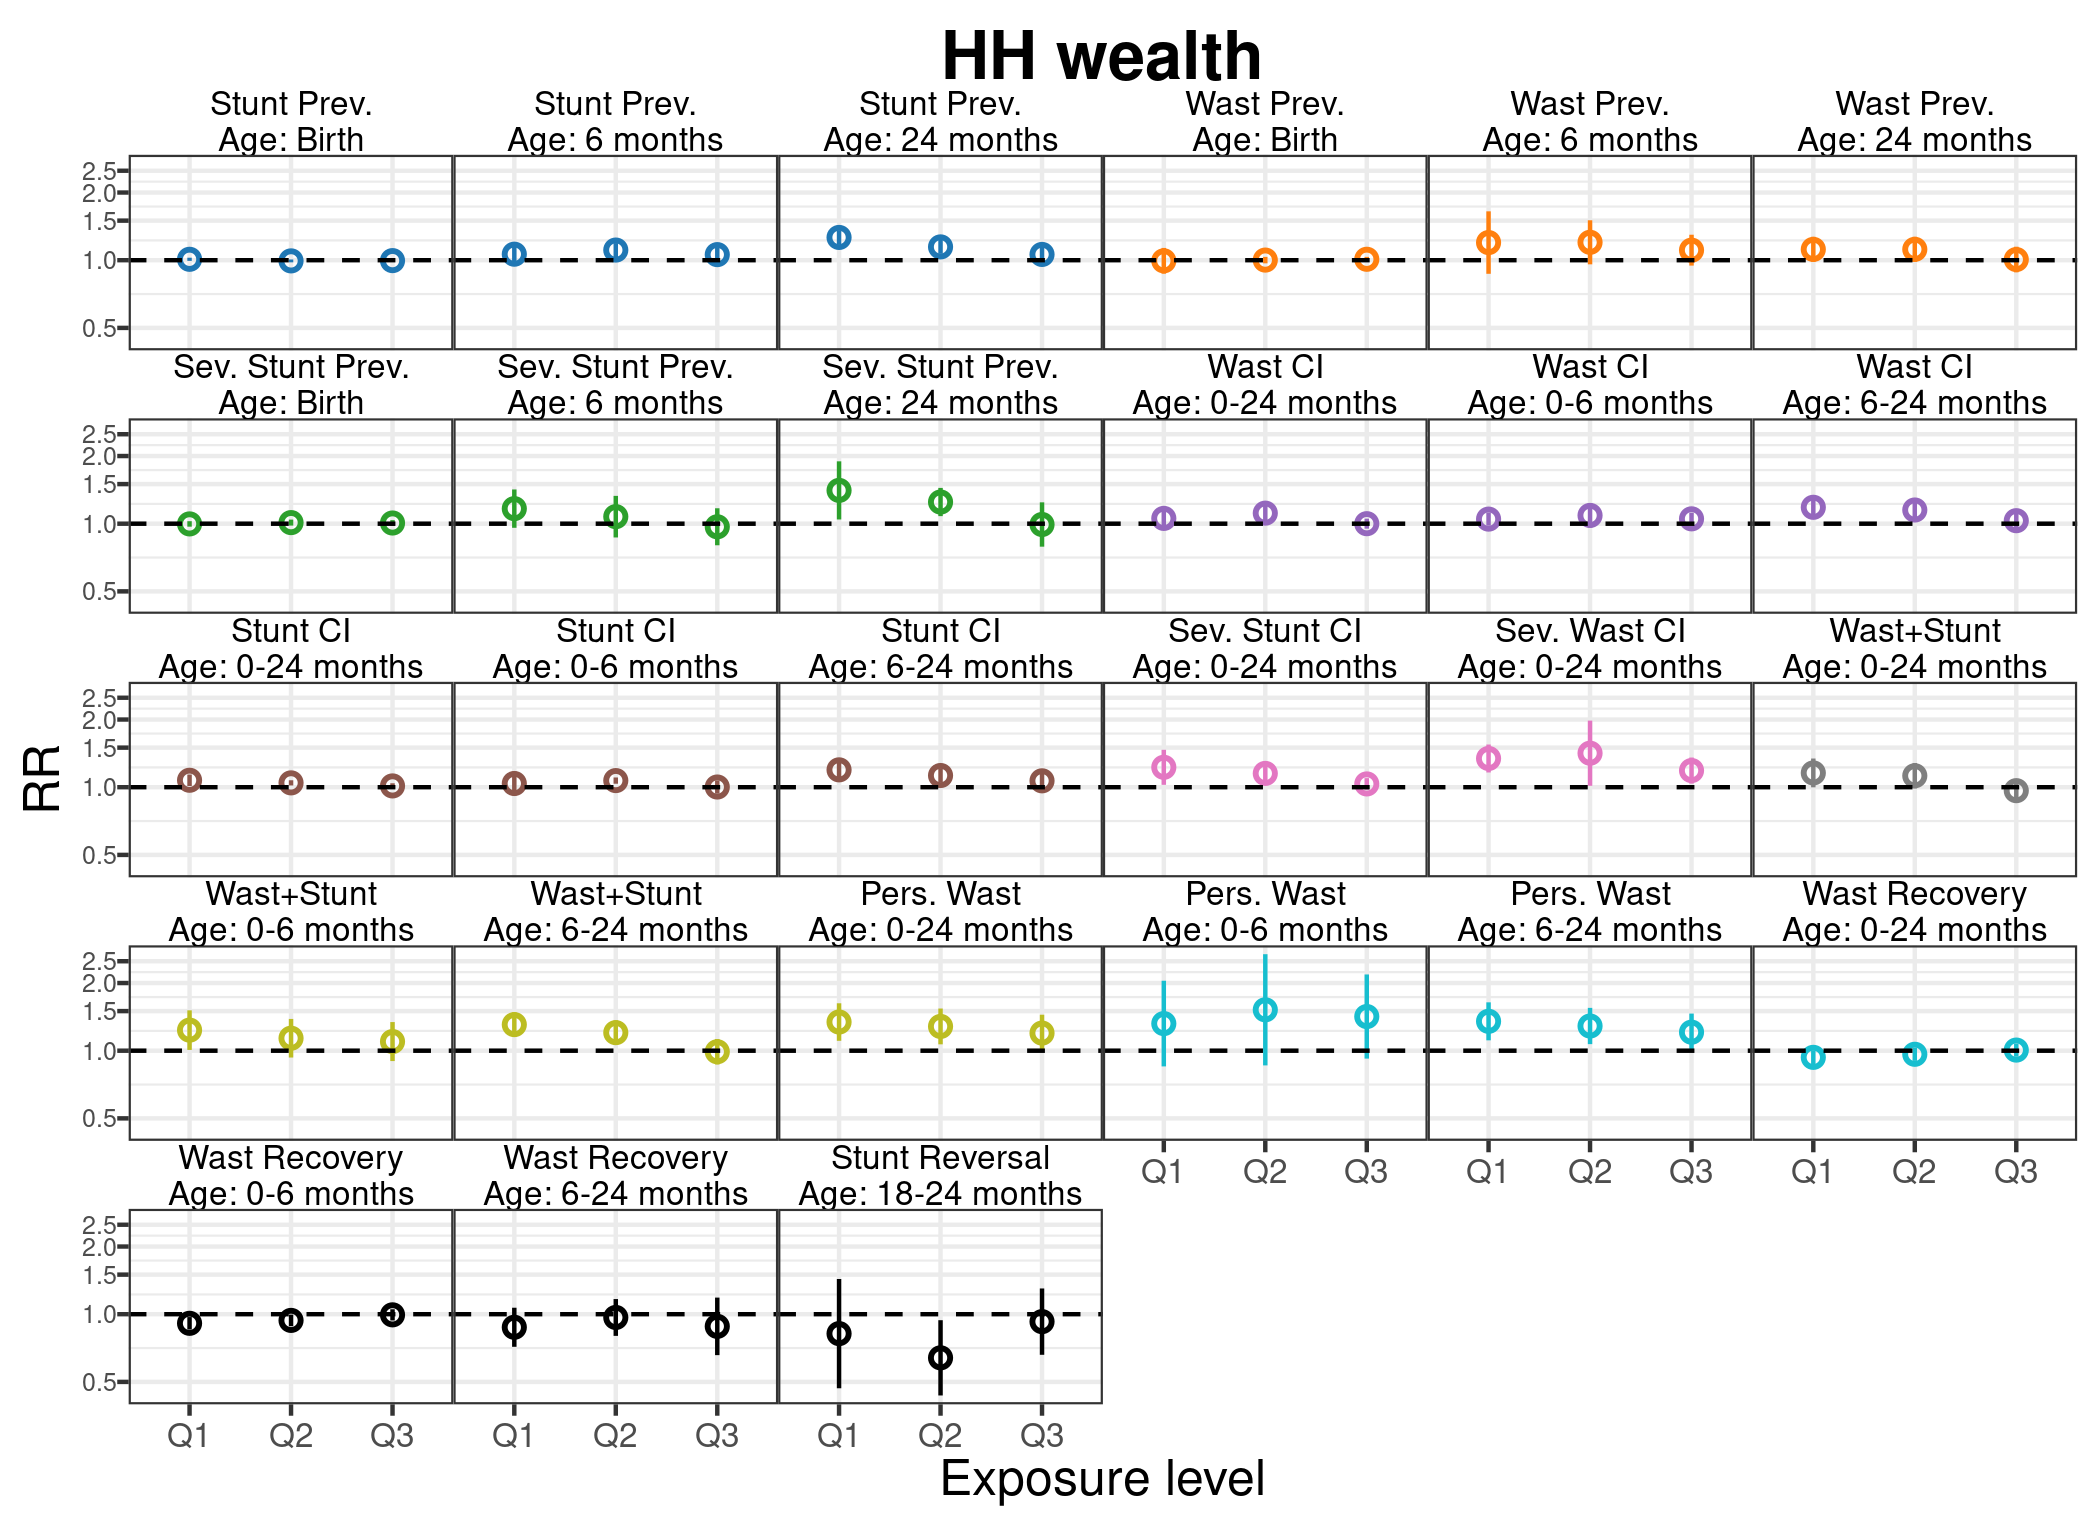
\includegraphics[width=58.33in]{C:/Users/andre/Documents/HBGDki/causes/ki-longitudinal-manuscripts/figures/risk-factor/RR-plots/fig-RR-hhwealth_quart}
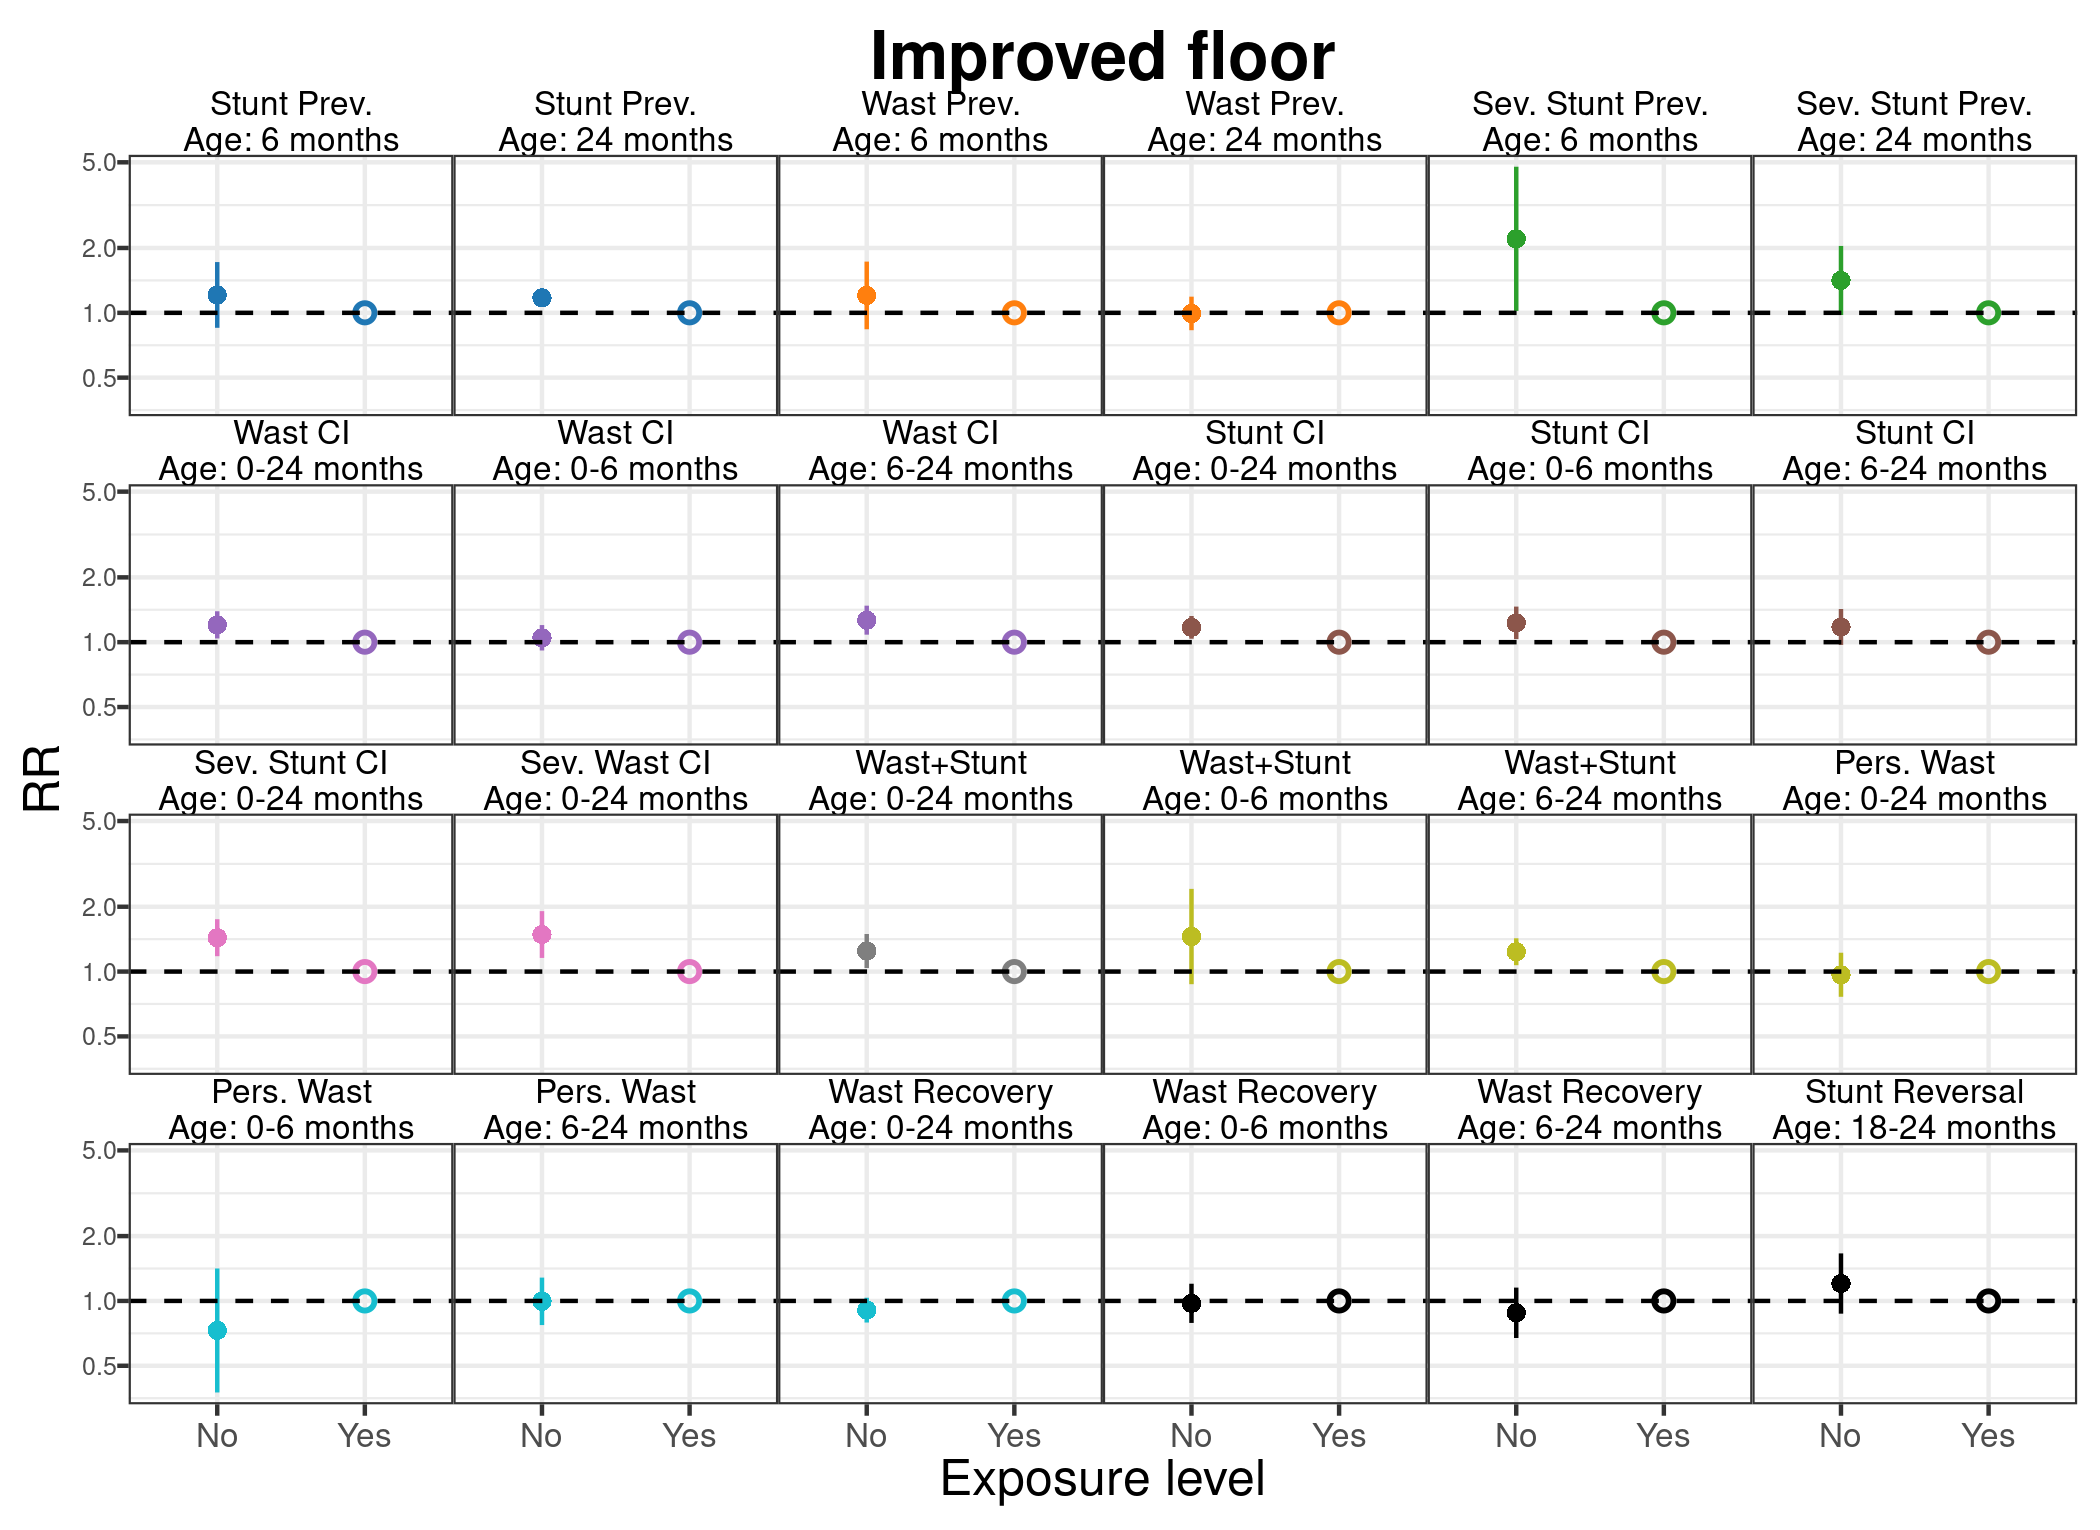
\includegraphics[width=58.33in]{C:/Users/andre/Documents/HBGDki/causes/ki-longitudinal-manuscripts/figures/risk-factor/RR-plots/fig-RR-impfloor}
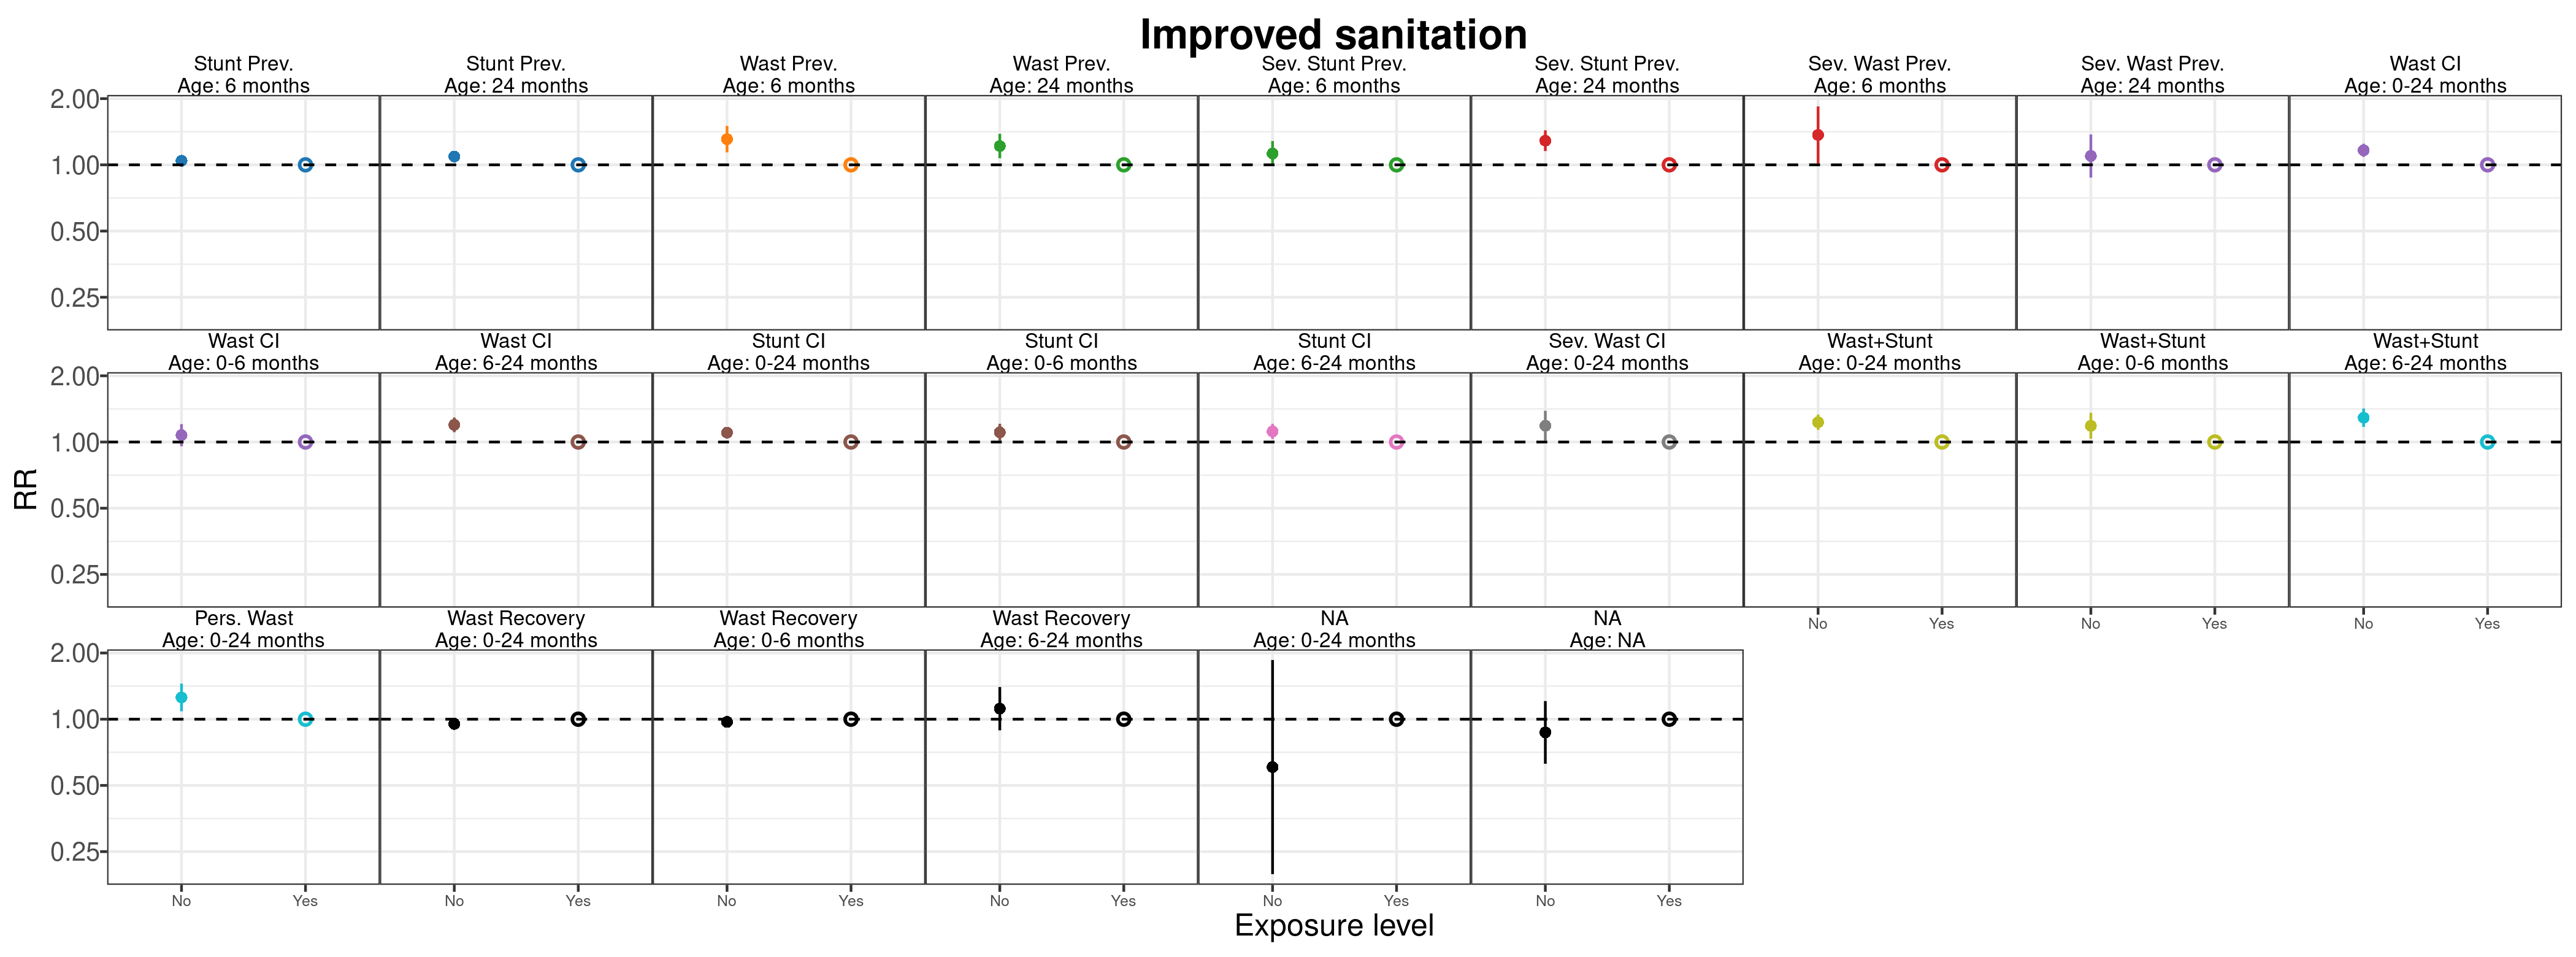
\includegraphics[width=58.33in]{C:/Users/andre/Documents/HBGDki/causes/ki-longitudinal-manuscripts/figures/risk-factor/RR-plots/fig-RR-impsan}
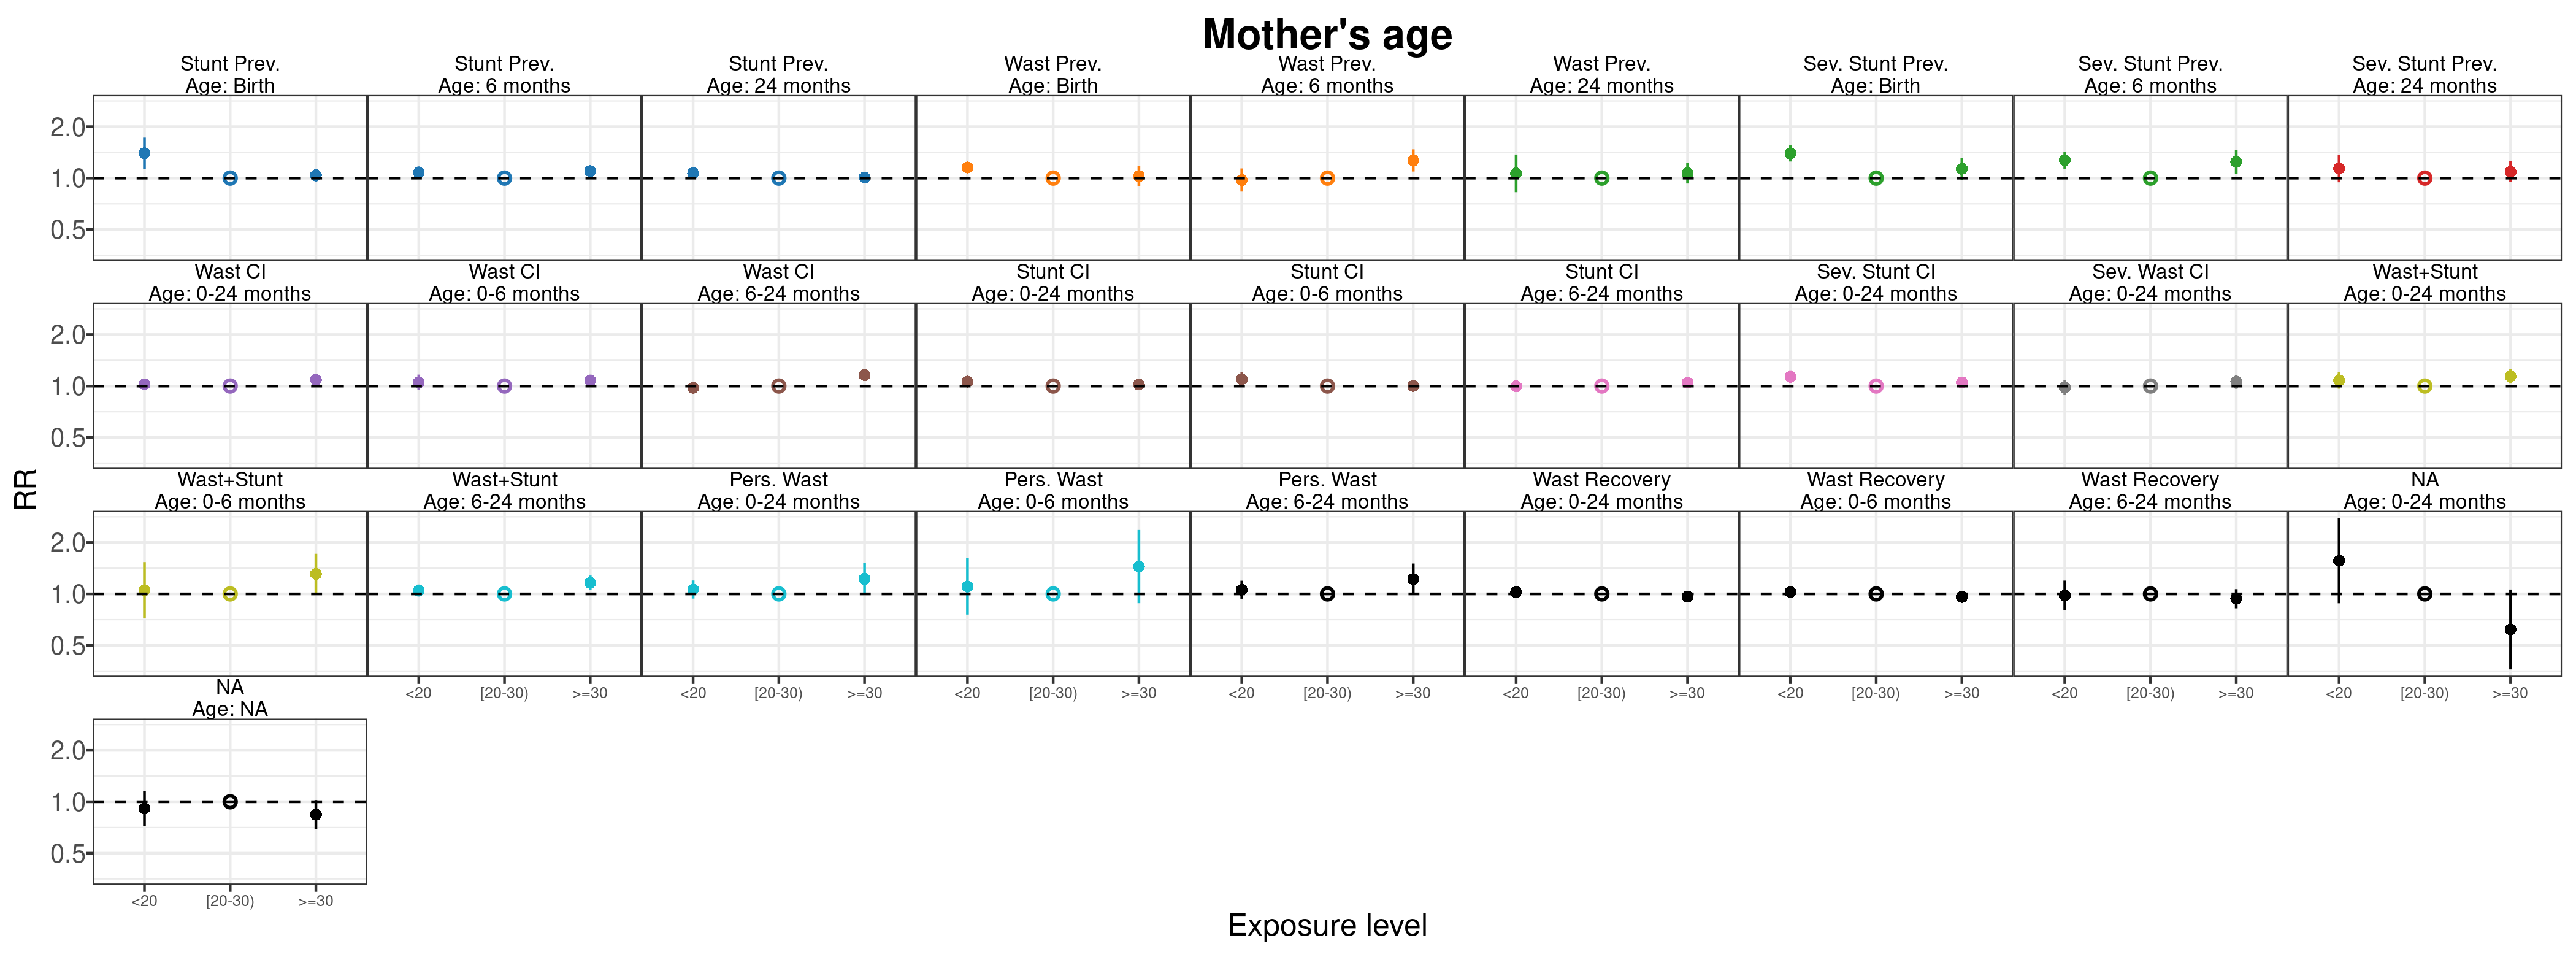
\includegraphics[width=58.33in]{C:/Users/andre/Documents/HBGDki/causes/ki-longitudinal-manuscripts/figures/risk-factor/RR-plots/fig-RR-mage}
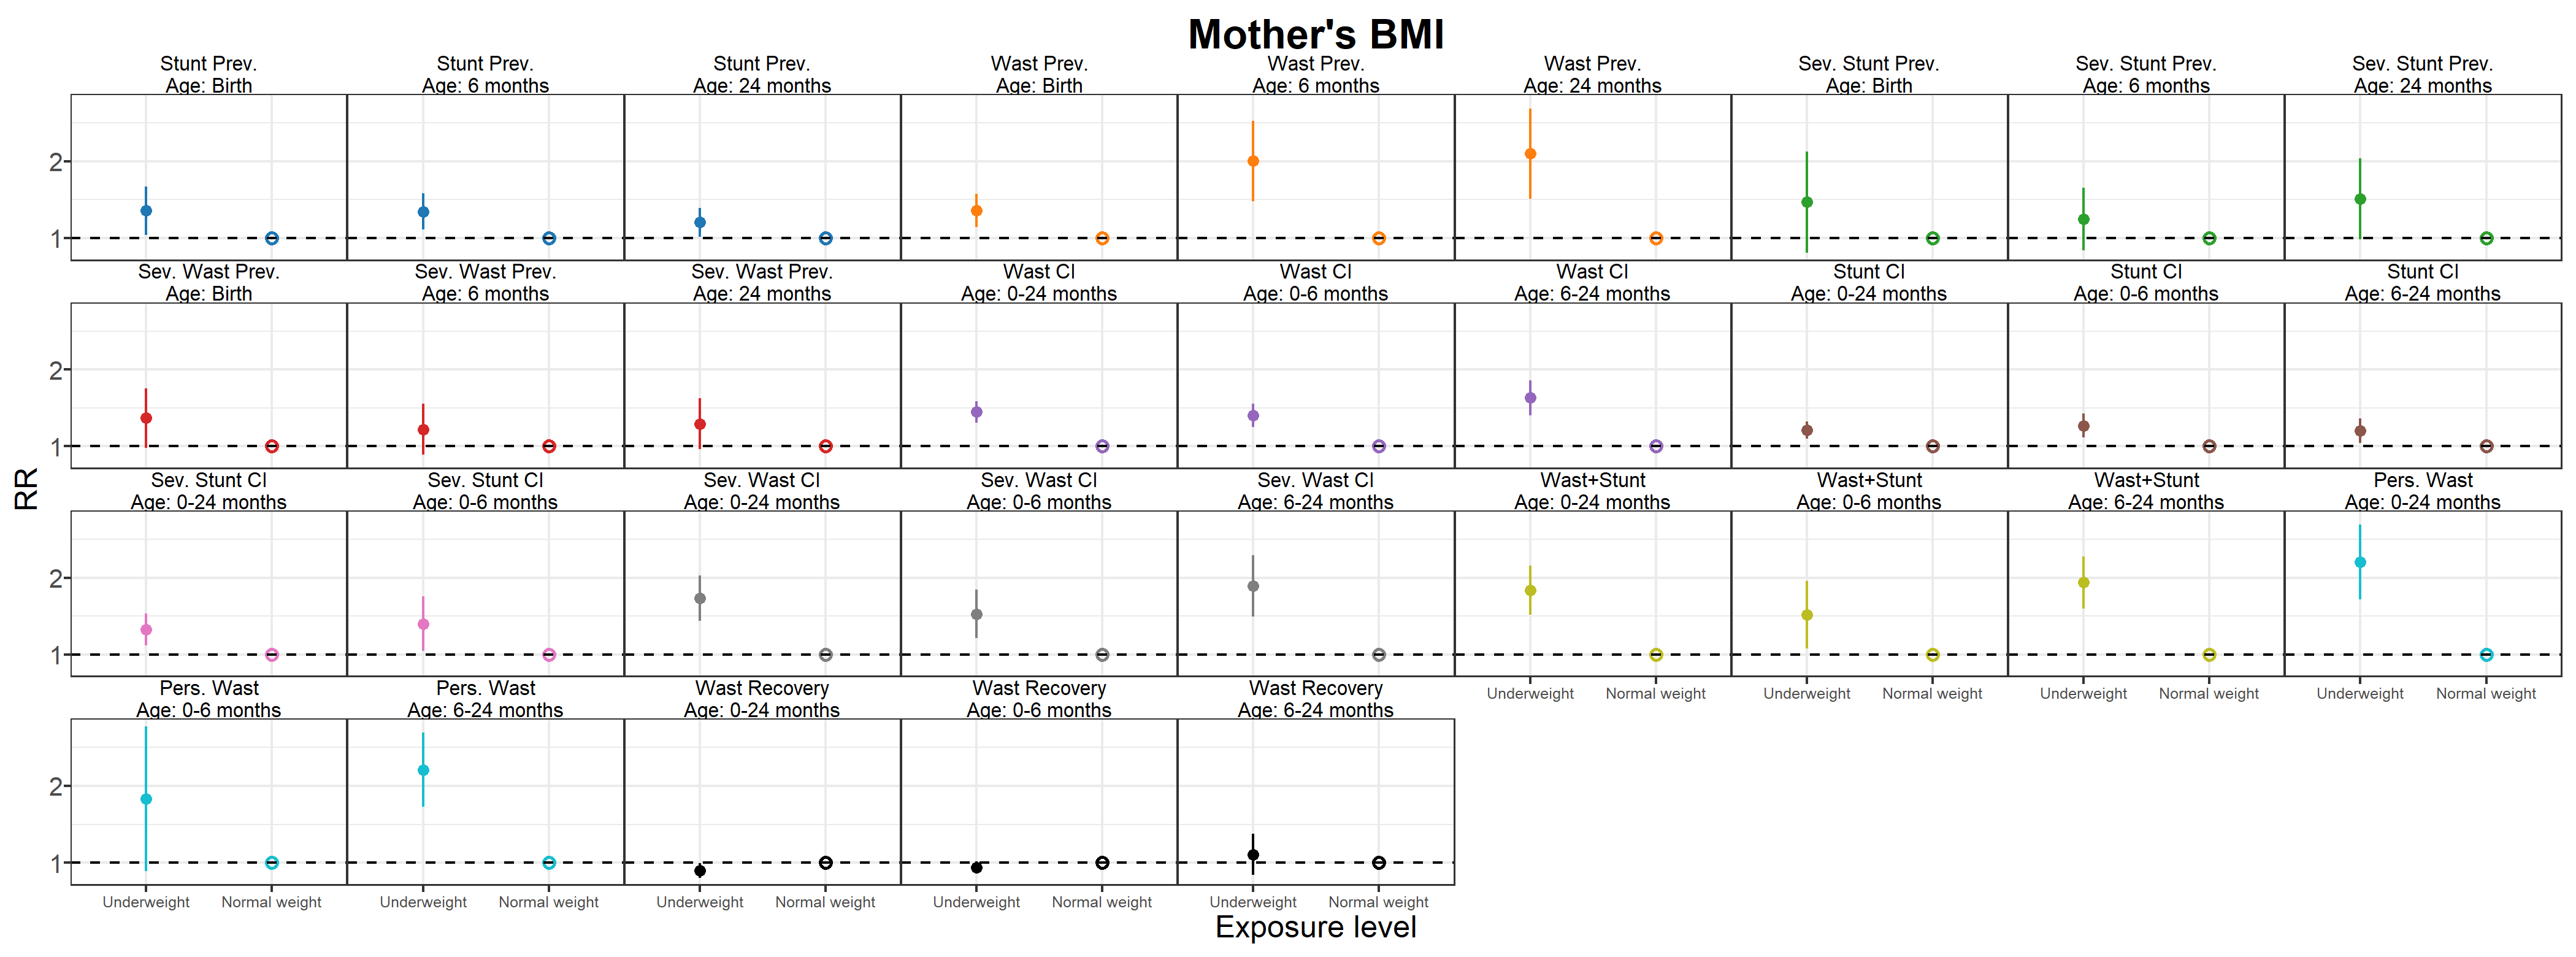
\includegraphics[width=58.33in]{C:/Users/andre/Documents/HBGDki/causes/ki-longitudinal-manuscripts/figures/risk-factor/RR-plots/fig-RR-mbmi}
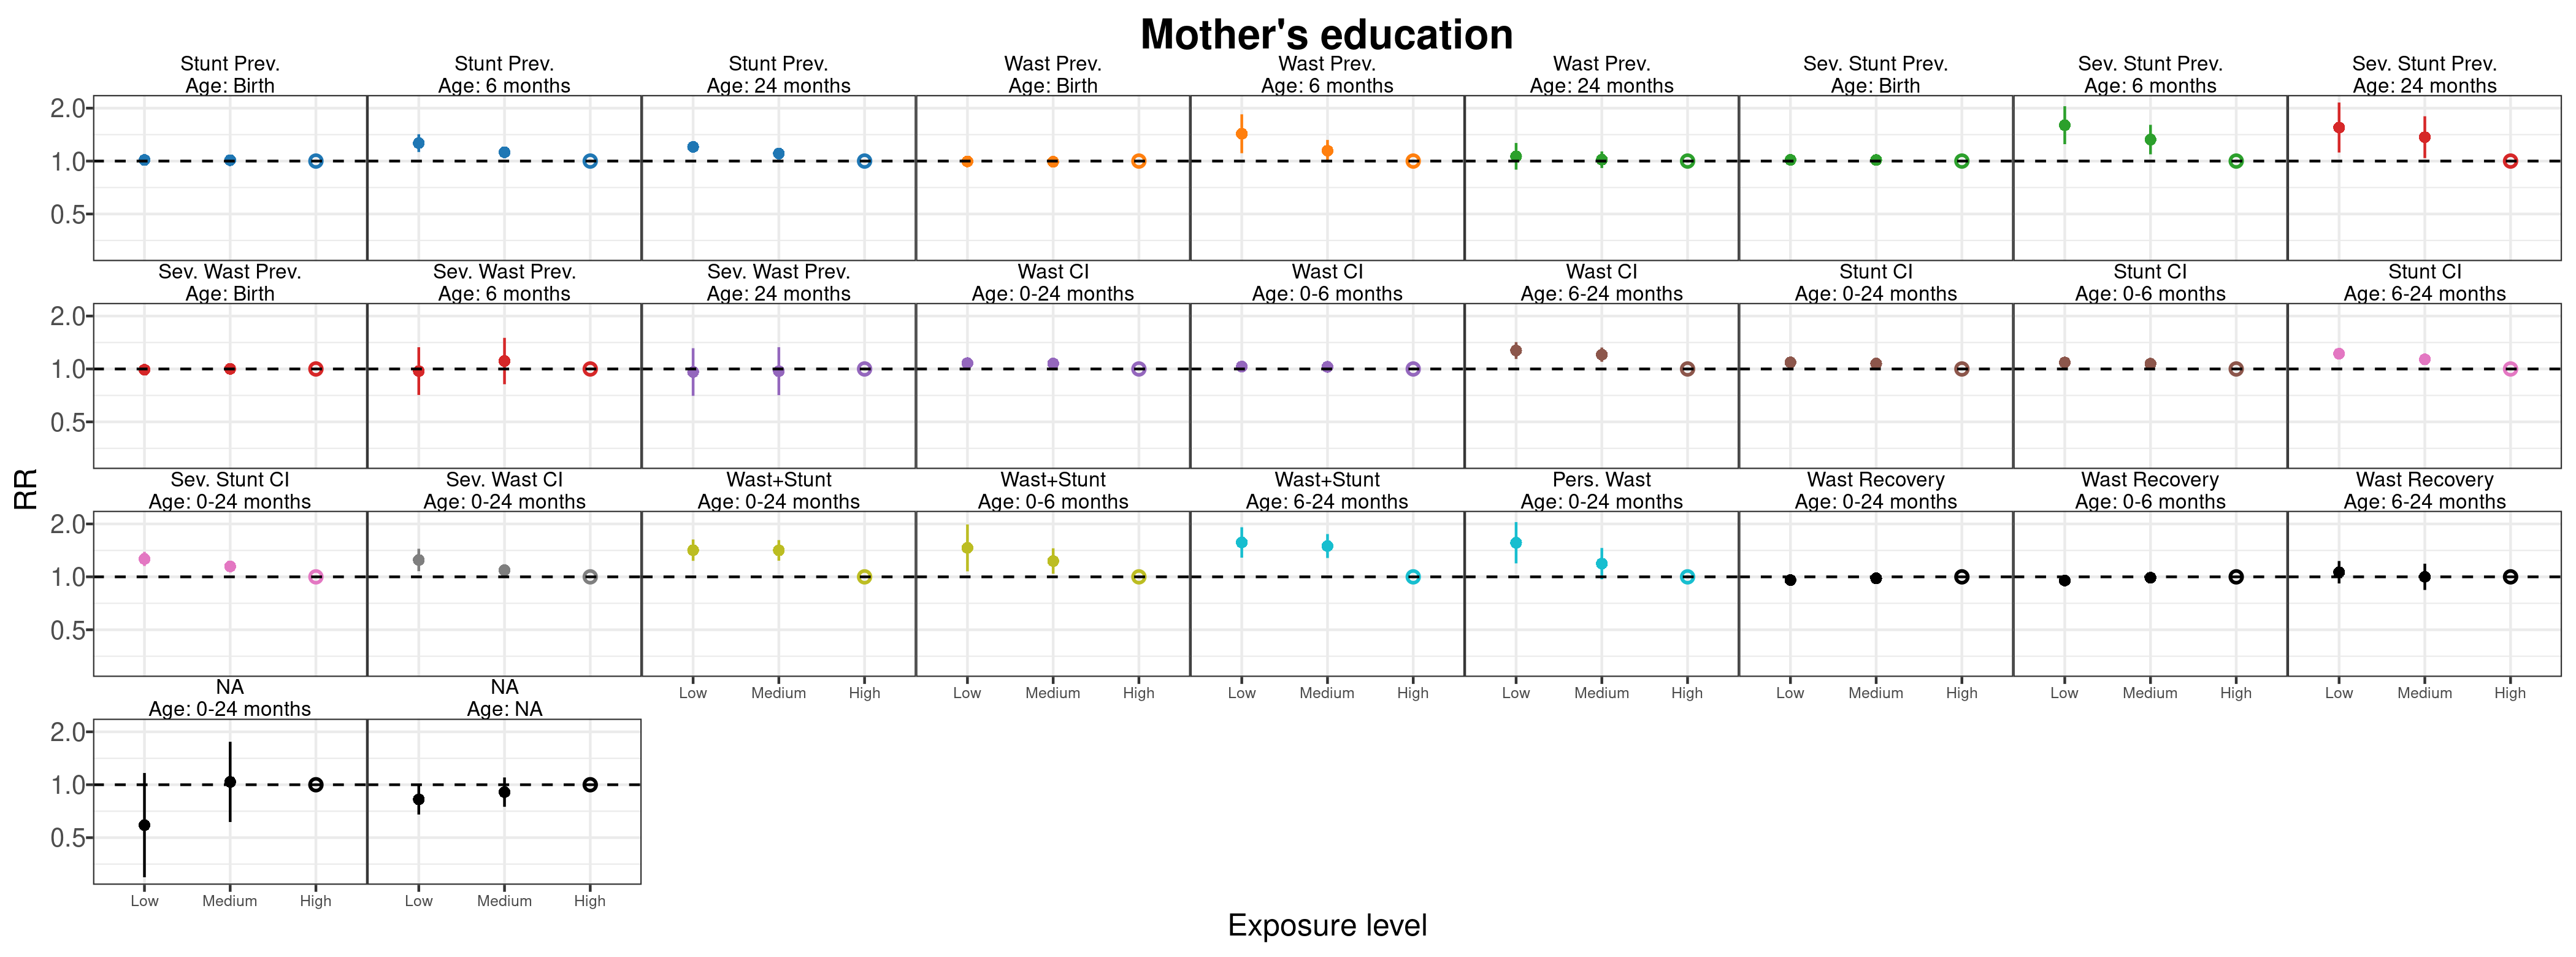
\includegraphics[width=58.33in]{C:/Users/andre/Documents/HBGDki/causes/ki-longitudinal-manuscripts/figures/risk-factor/RR-plots/fig-RR-meducyrs}
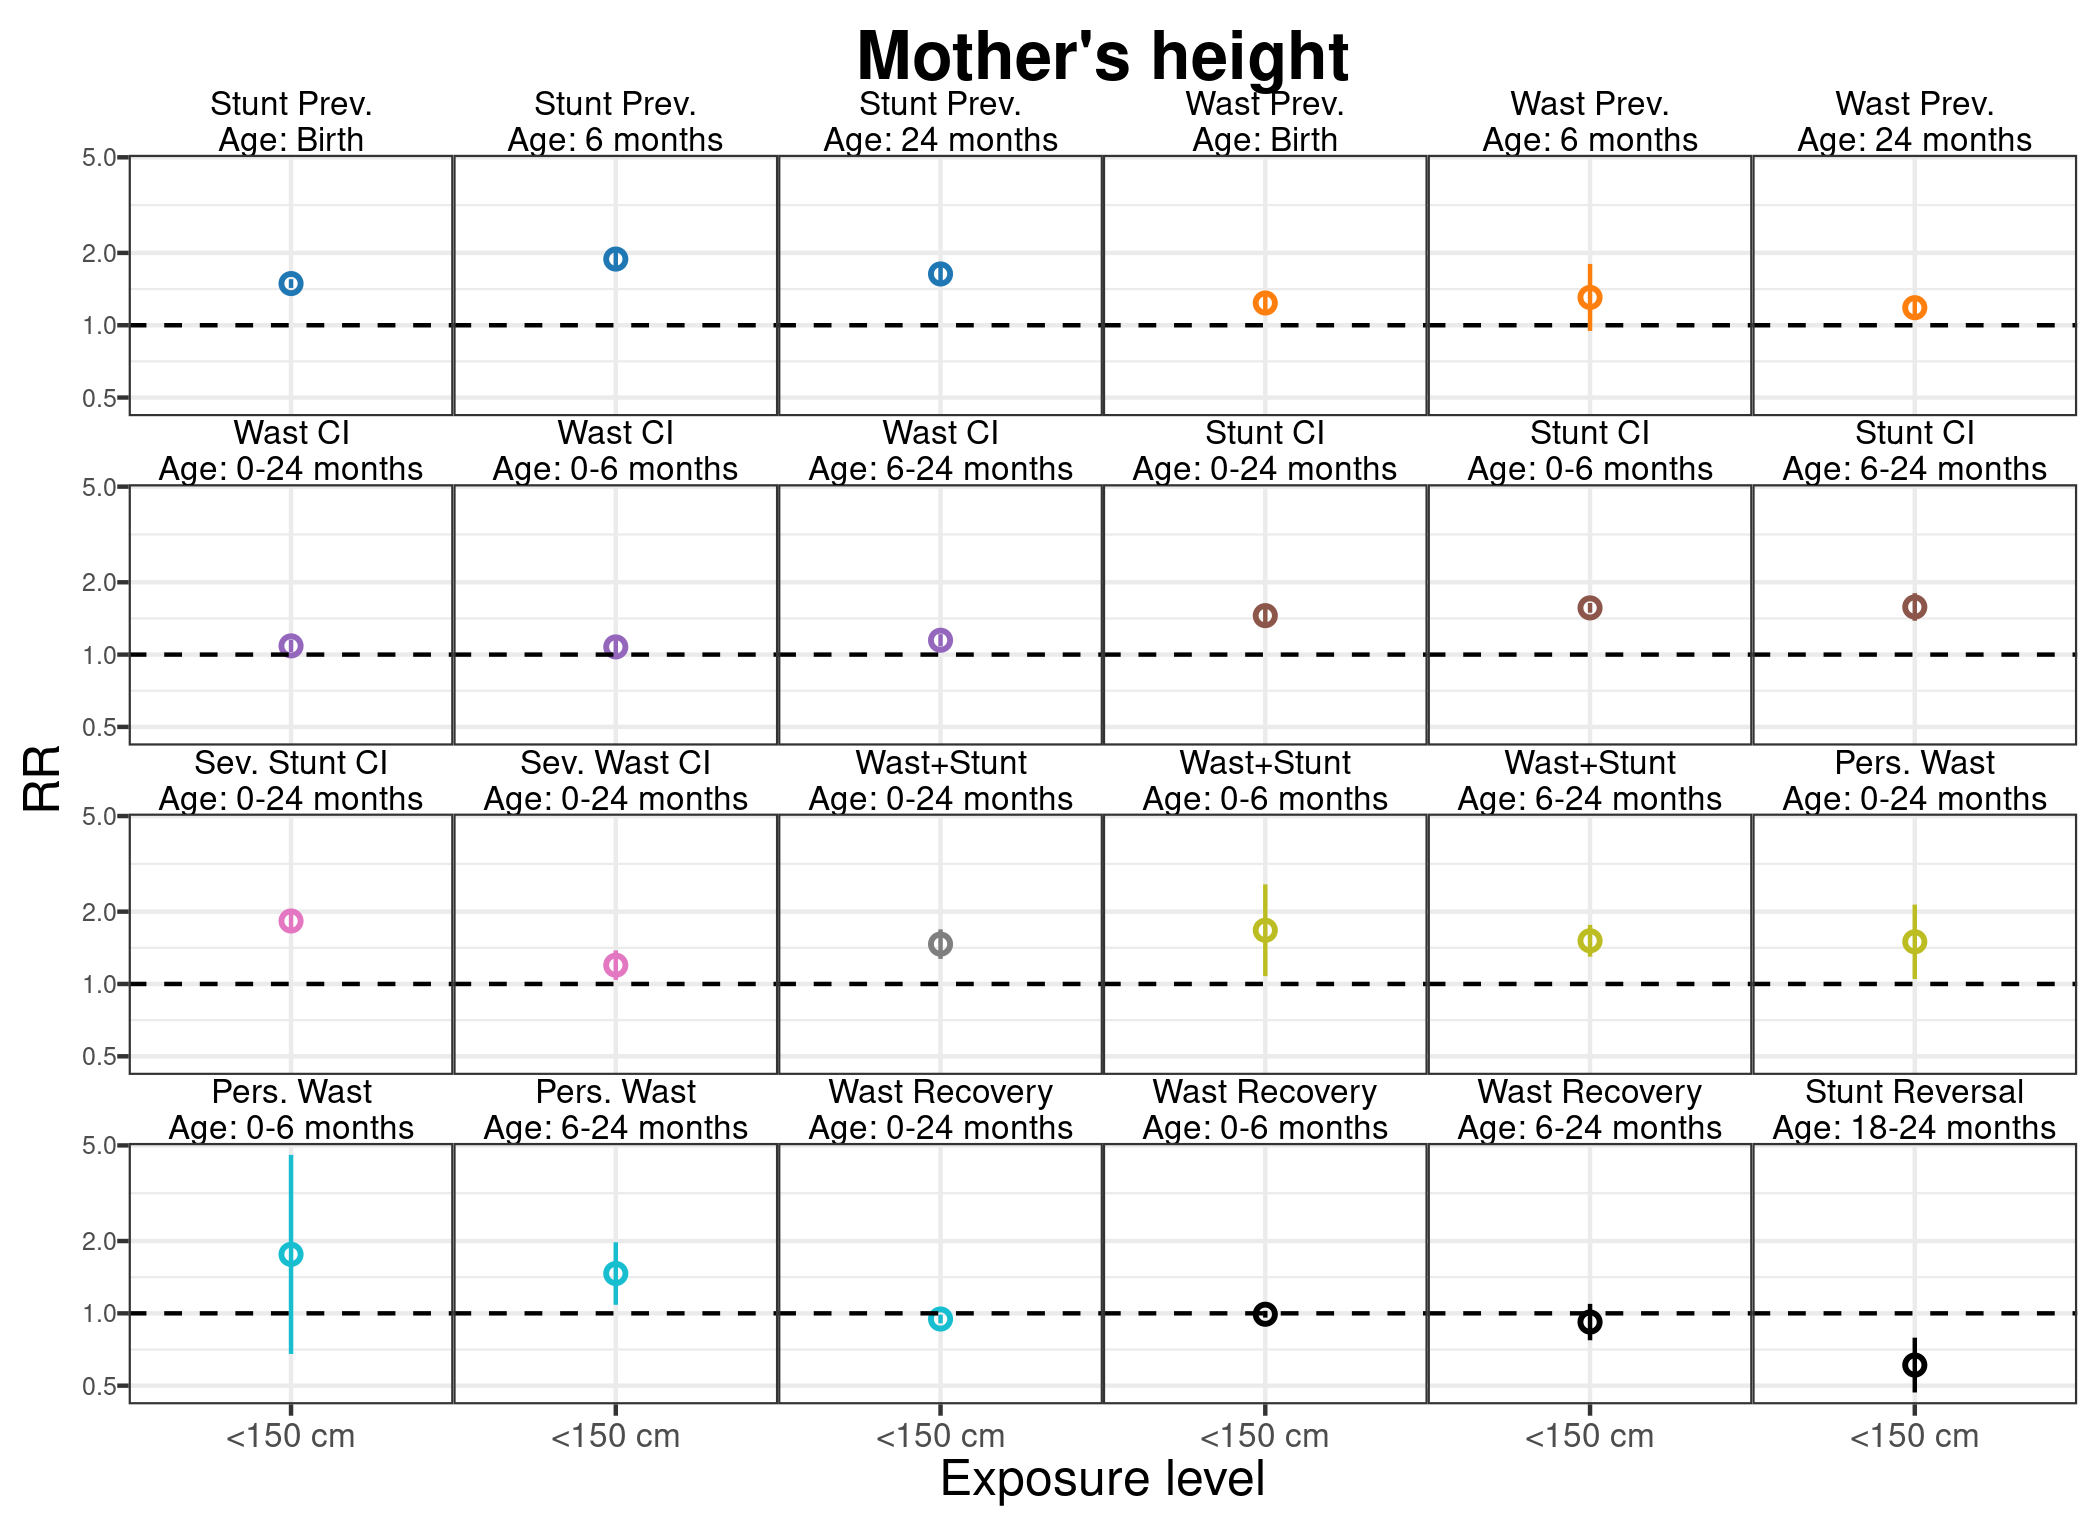
\includegraphics[width=58.33in]{C:/Users/andre/Documents/HBGDki/causes/ki-longitudinal-manuscripts/figures/risk-factor/RR-plots/fig-RR-mhtcm}
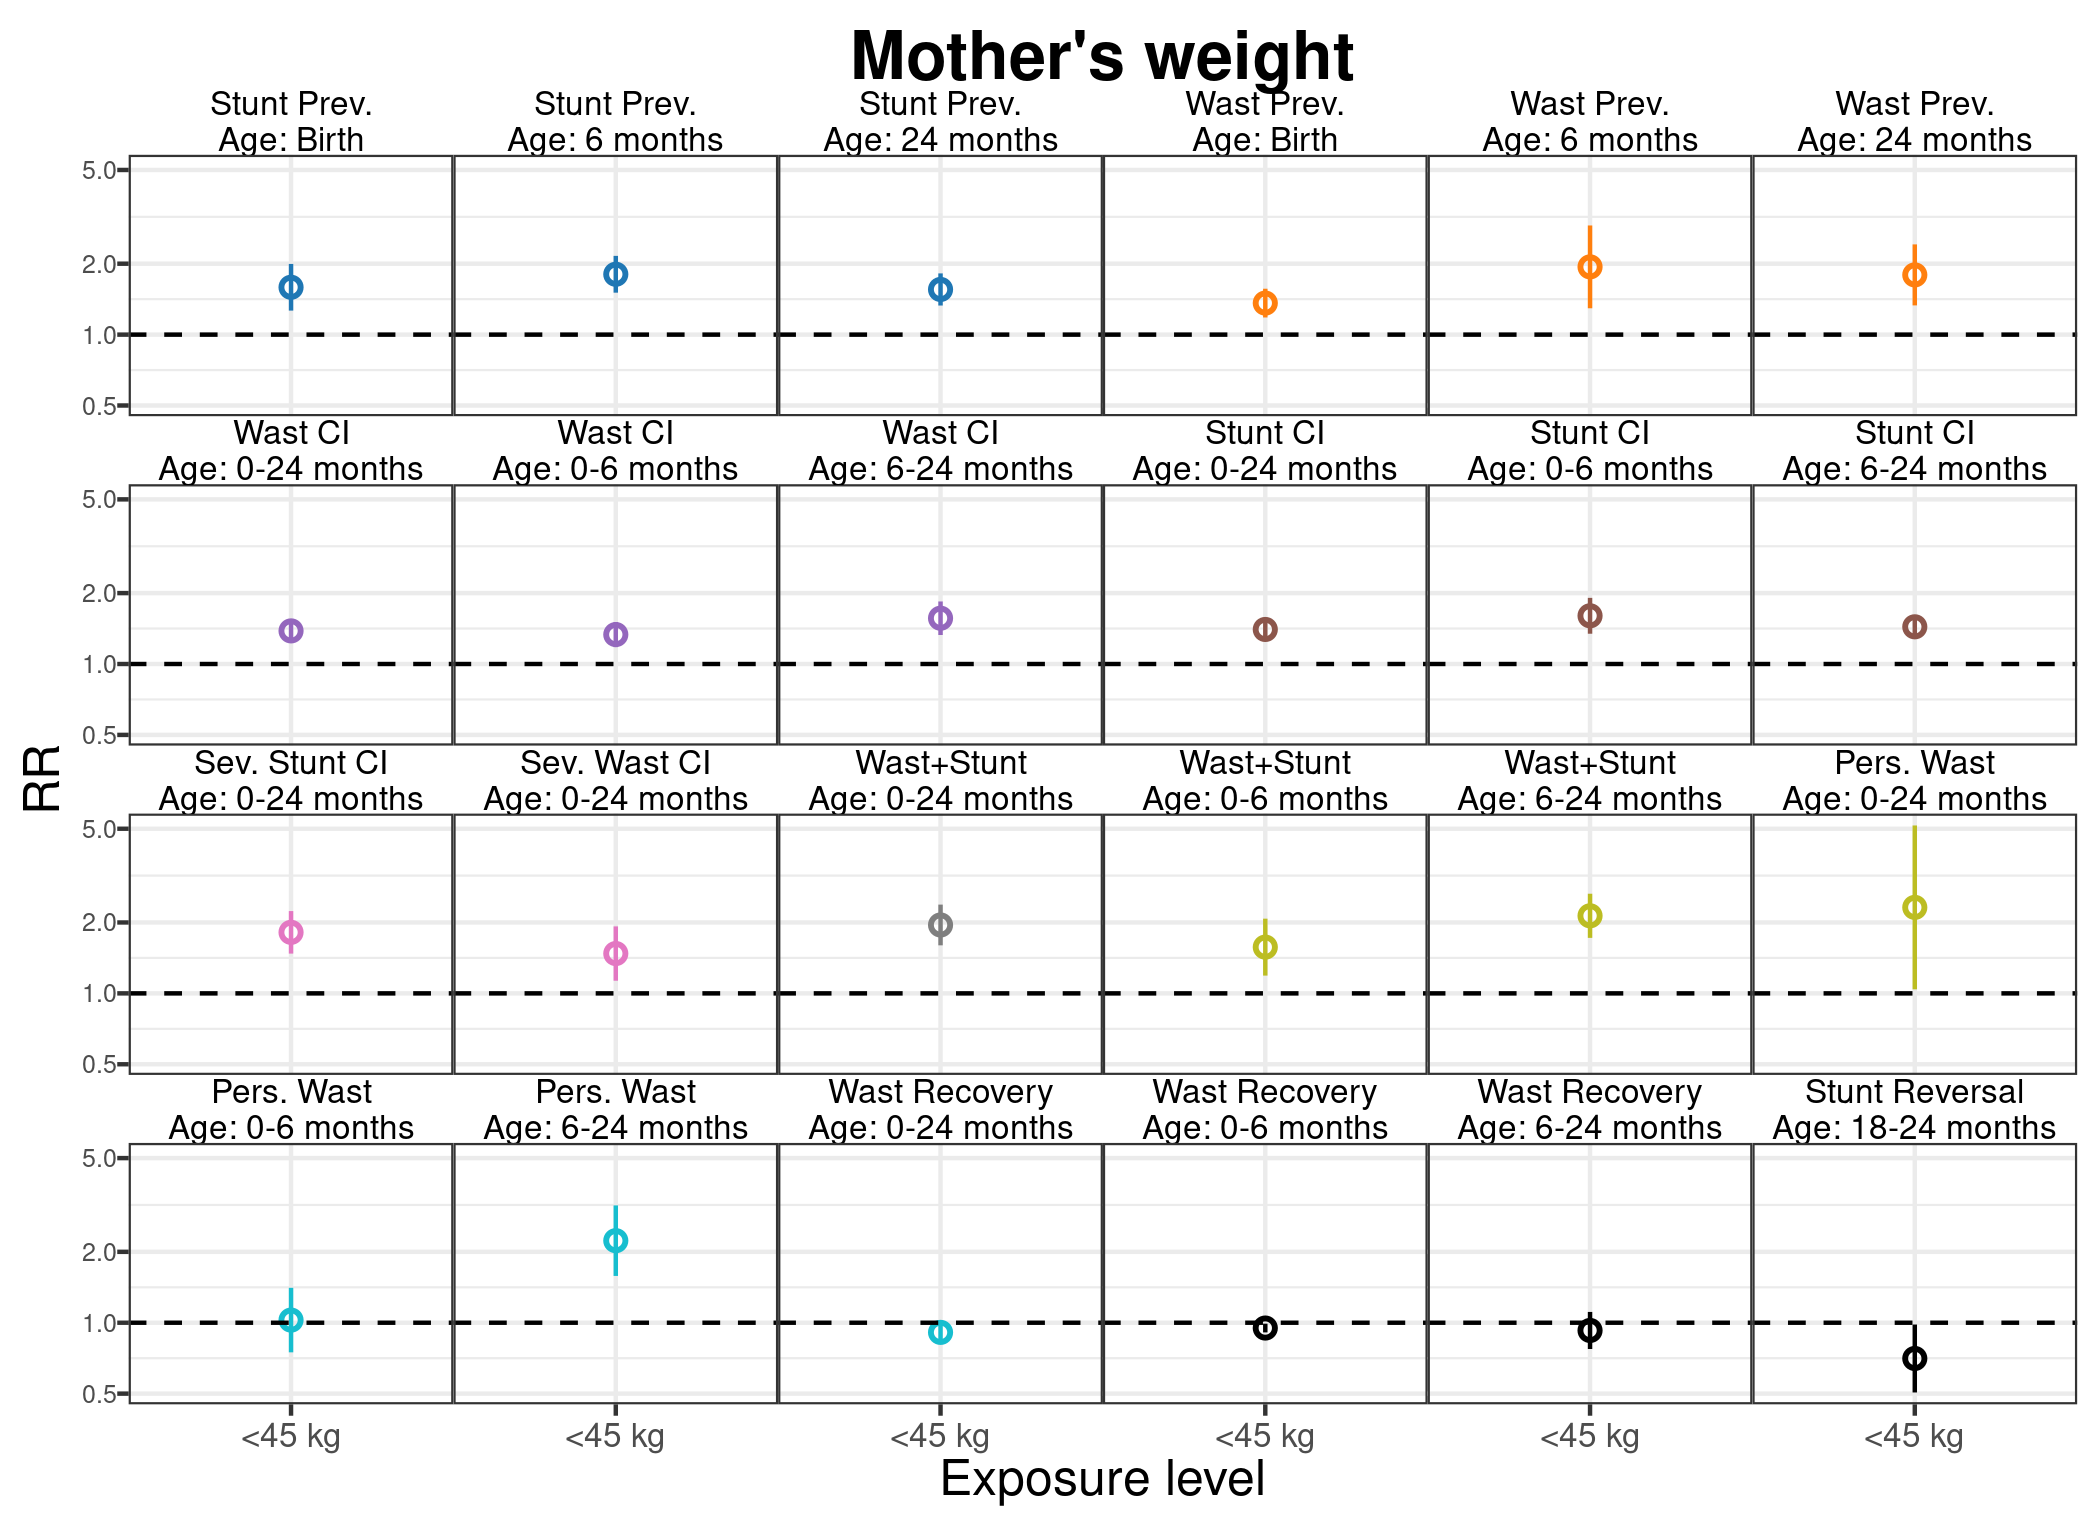
\includegraphics[width=58.33in]{C:/Users/andre/Documents/HBGDki/causes/ki-longitudinal-manuscripts/figures/risk-factor/RR-plots/fig-RR-mwtkg}
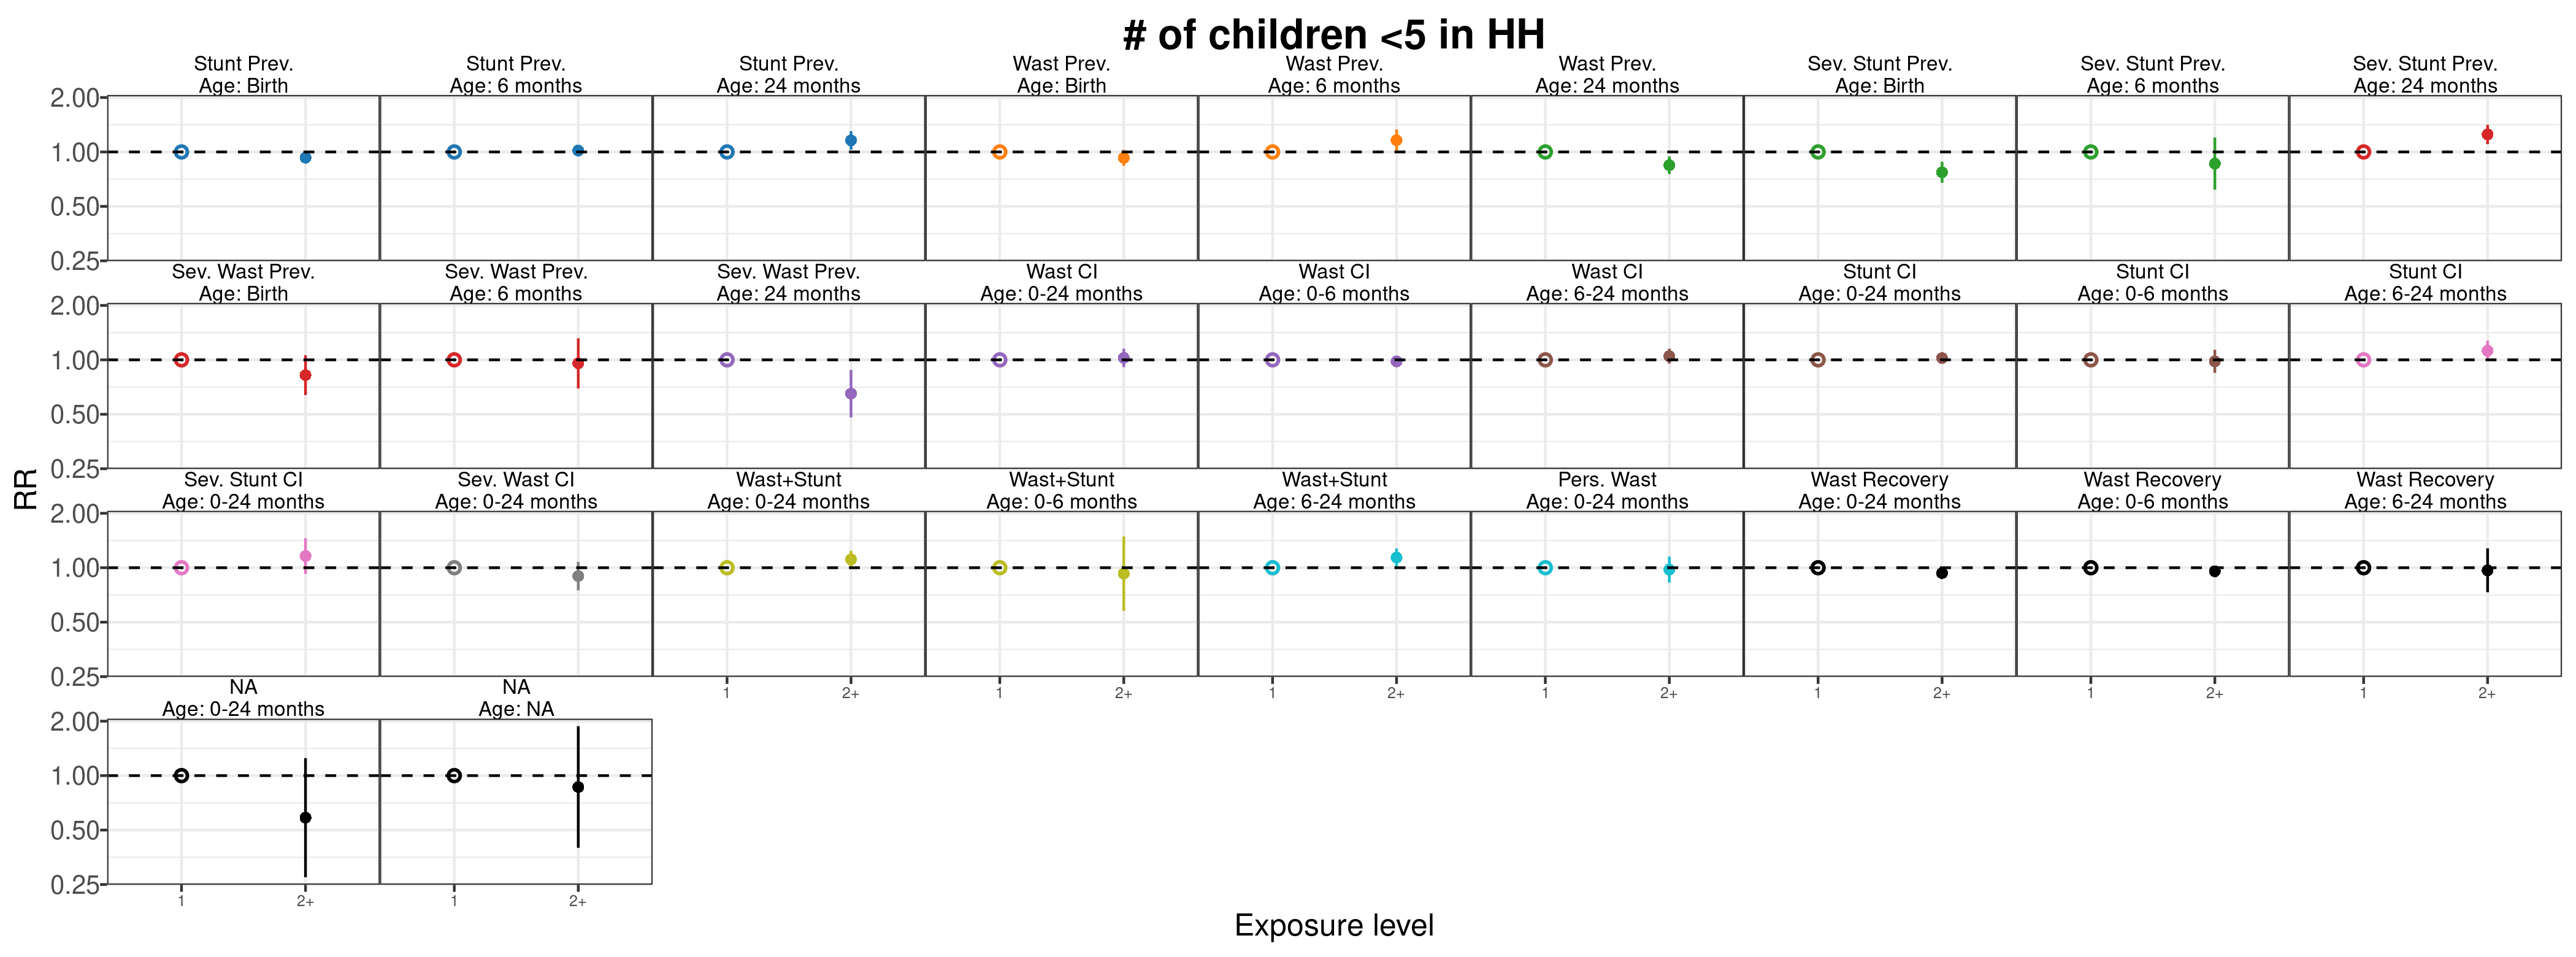
\includegraphics[width=58.33in]{C:/Users/andre/Documents/HBGDki/causes/ki-longitudinal-manuscripts/figures/risk-factor/RR-plots/fig-RR-nchldlt5}
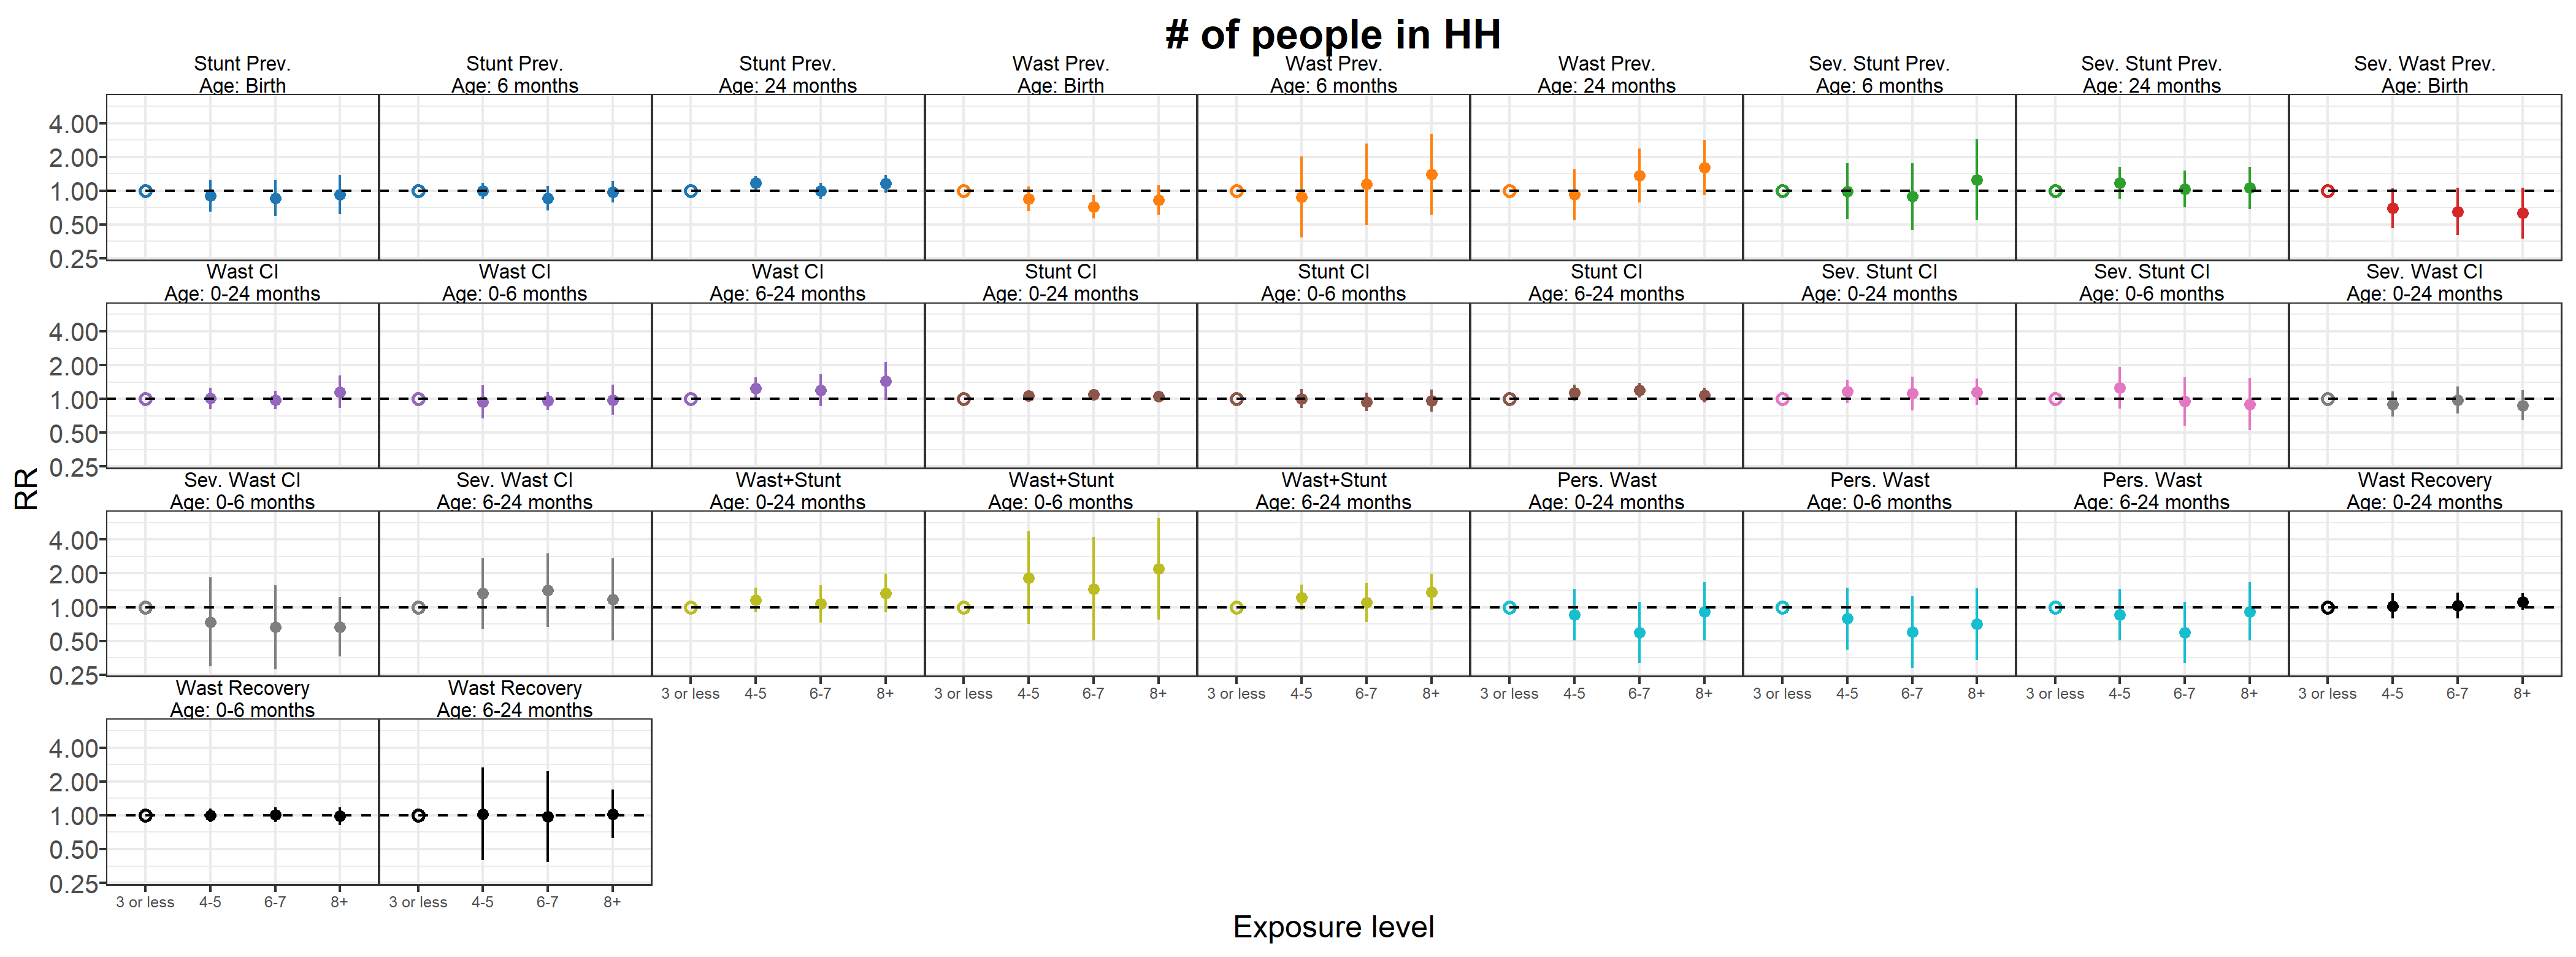
\includegraphics[width=58.33in]{C:/Users/andre/Documents/HBGDki/causes/ki-longitudinal-manuscripts/figures/risk-factor/RR-plots/fig-RR-nhh}
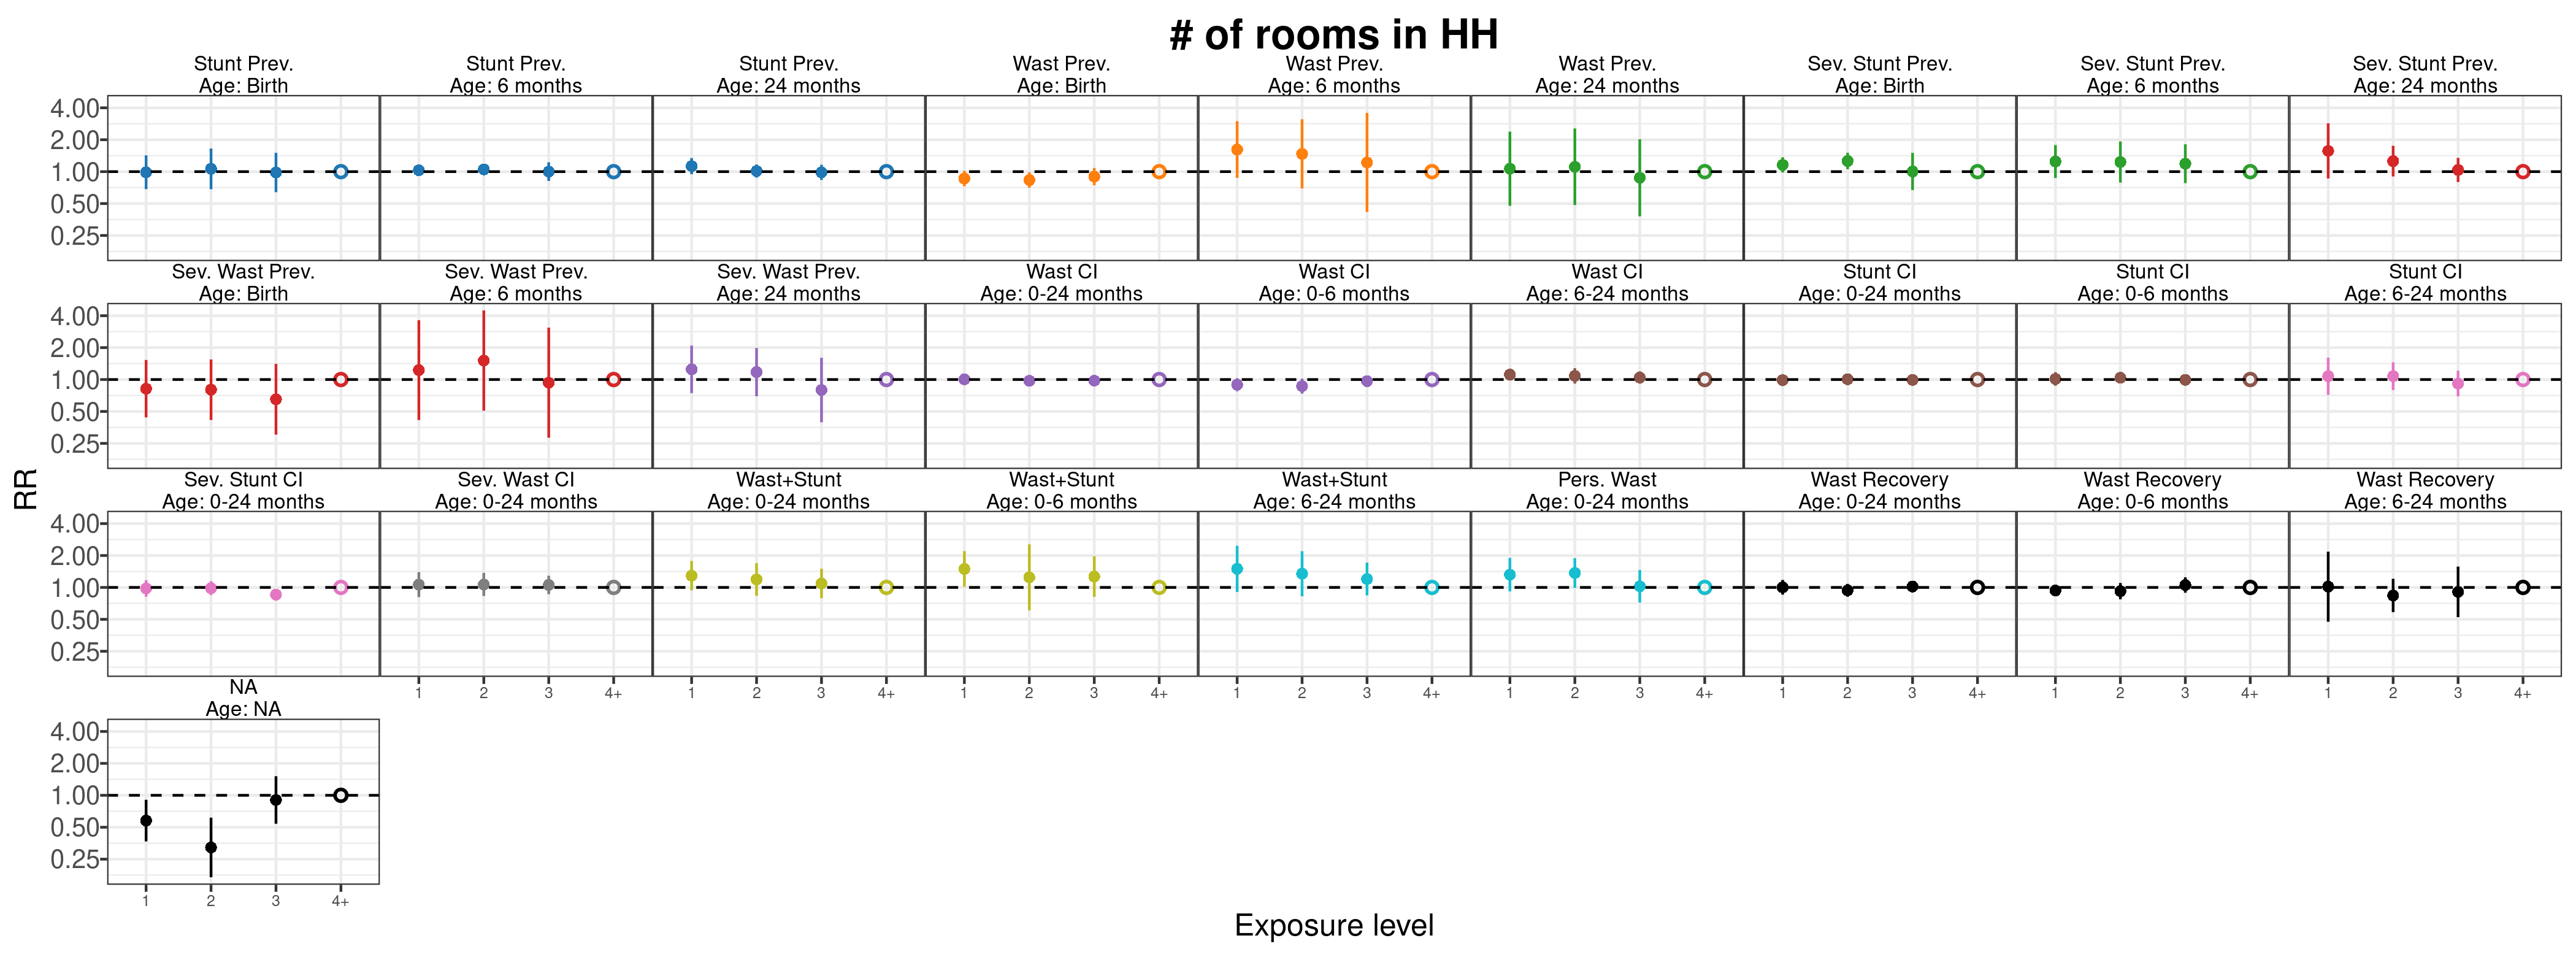
\includegraphics[width=58.33in]{C:/Users/andre/Documents/HBGDki/causes/ki-longitudinal-manuscripts/figures/risk-factor/RR-plots/fig-RR-nrooms}
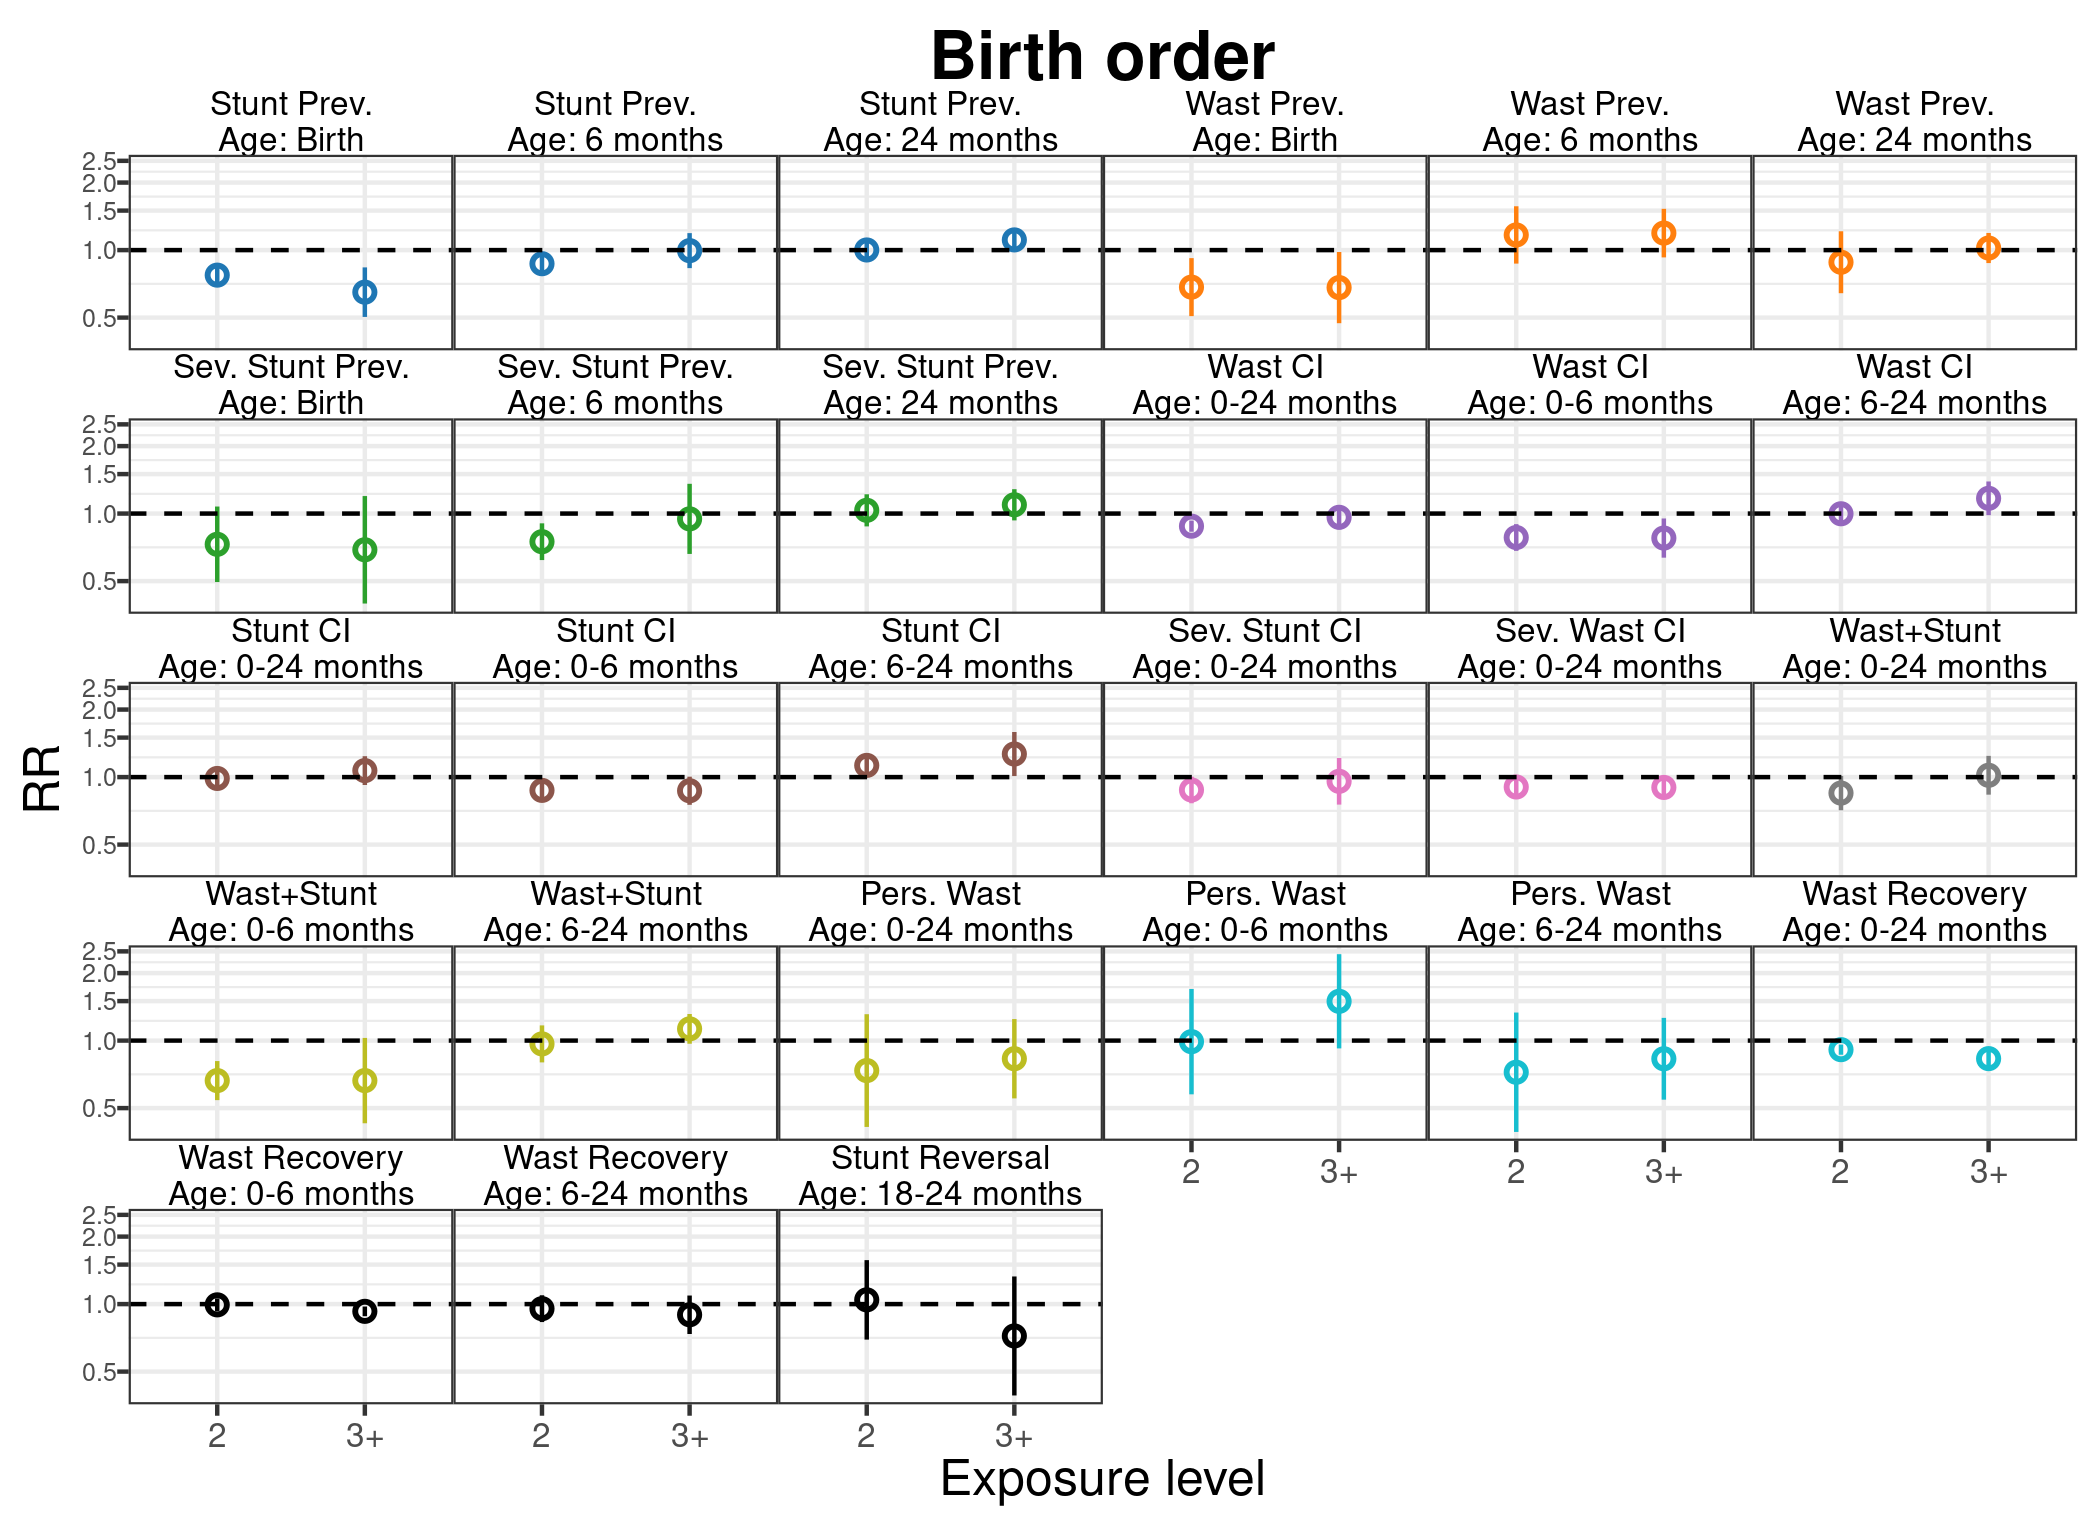
\includegraphics[width=58.33in]{C:/Users/andre/Documents/HBGDki/causes/ki-longitudinal-manuscripts/figures/risk-factor/RR-plots/fig-RR-parity}
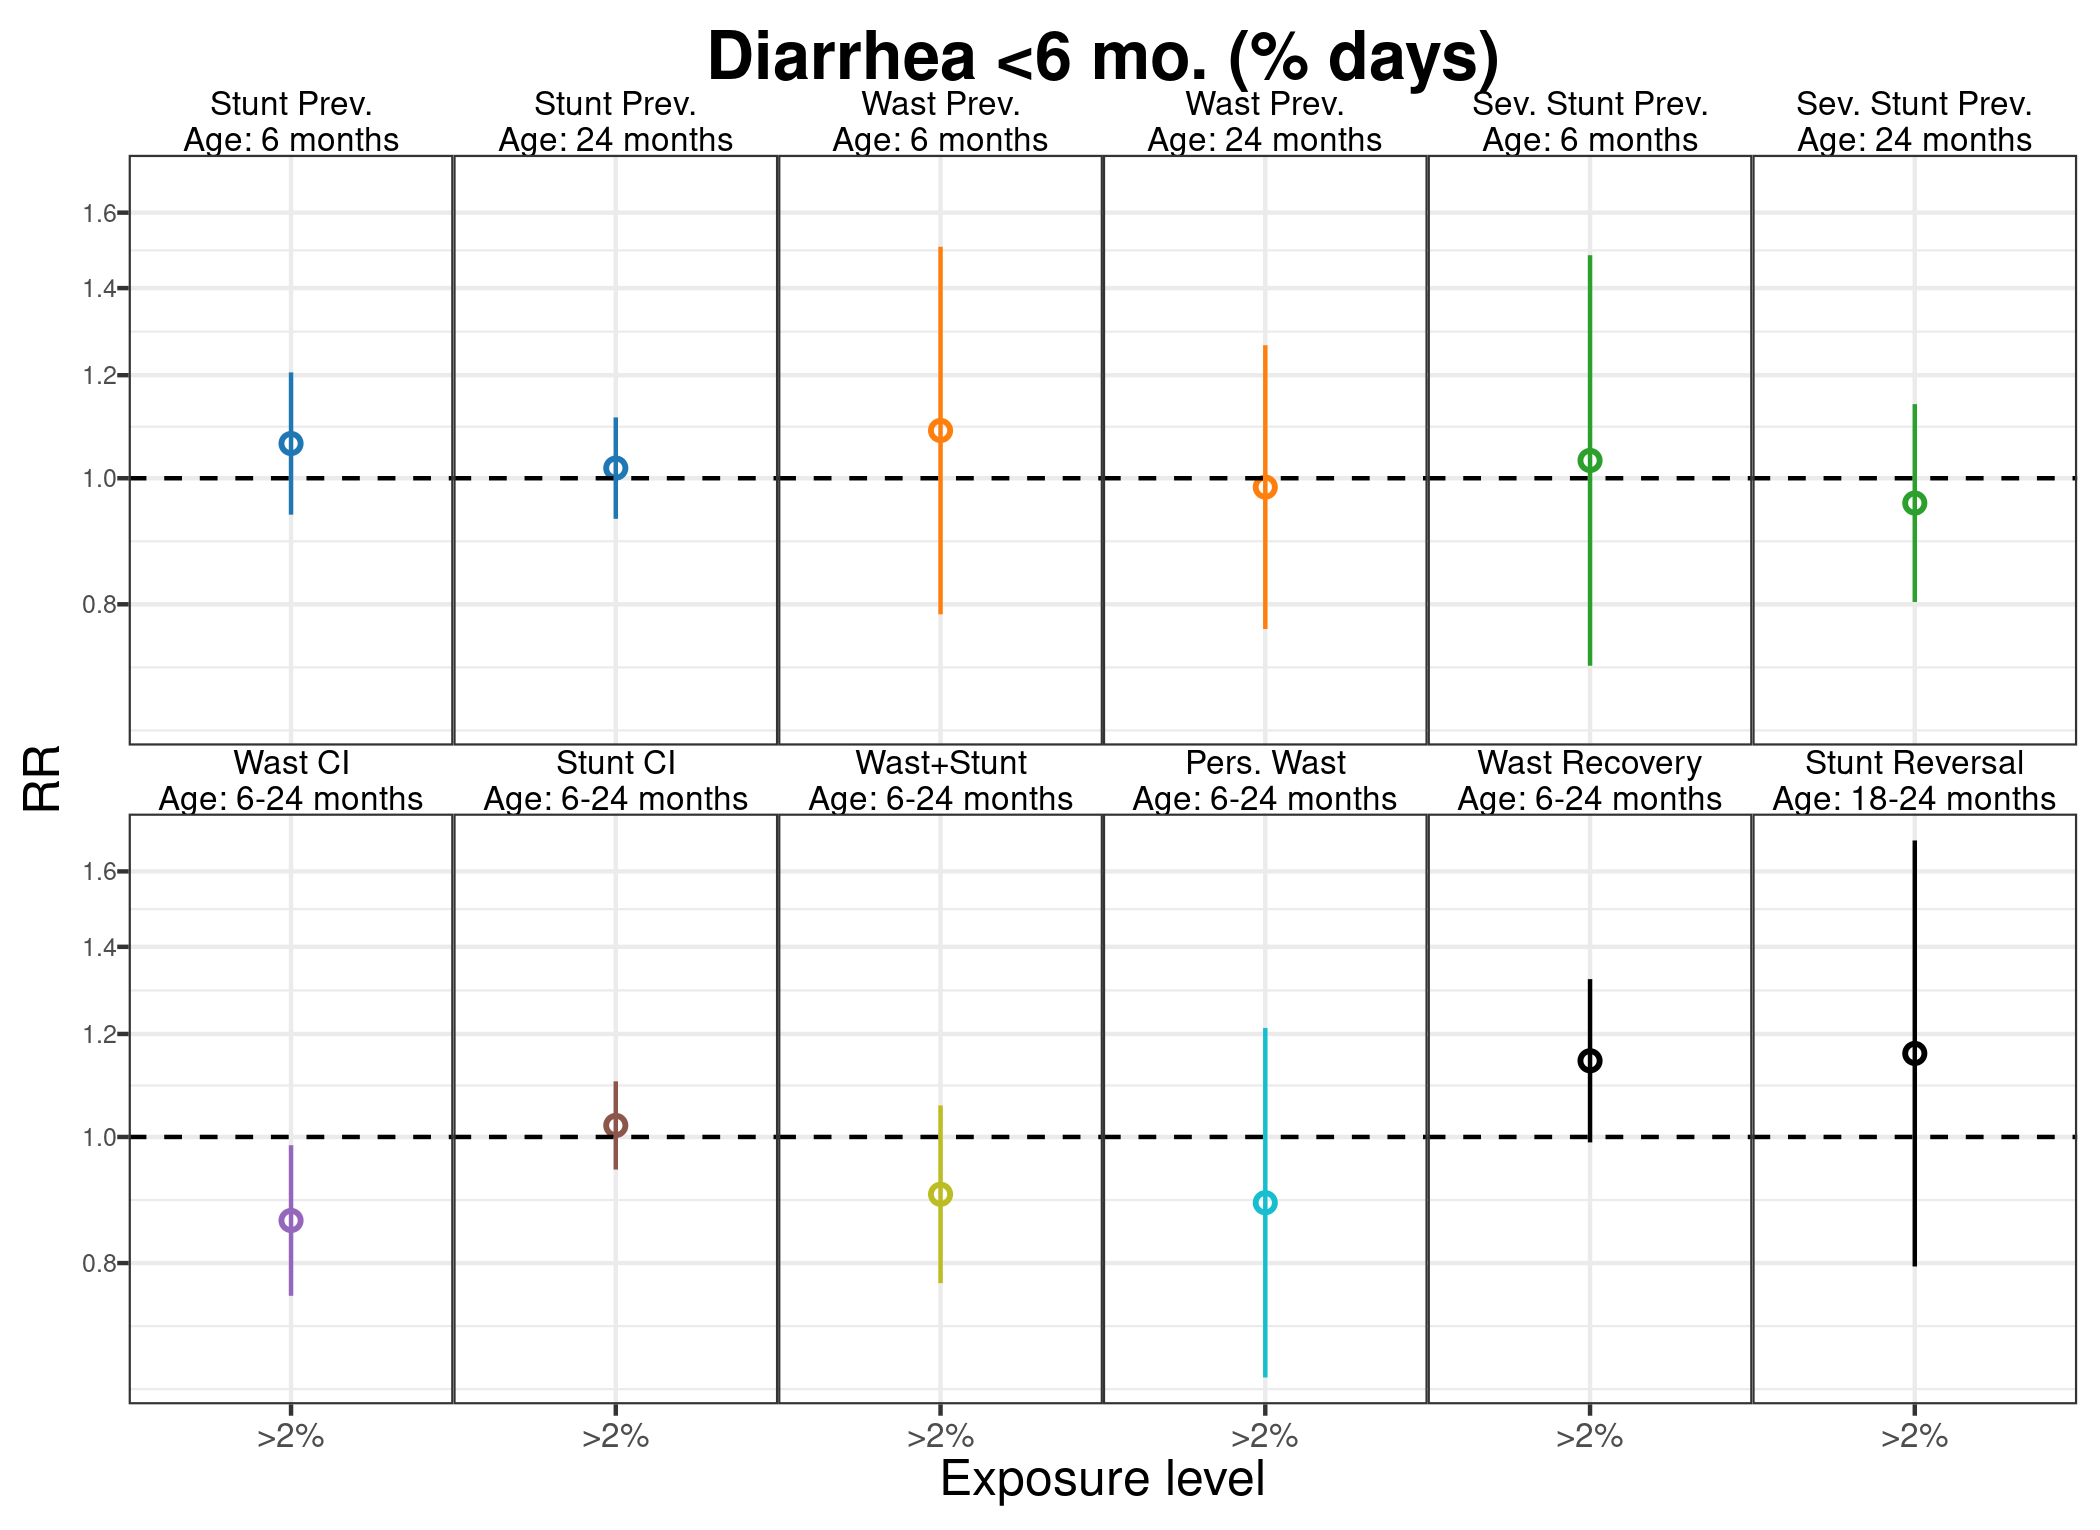
\includegraphics[width=58.33in]{C:/Users/andre/Documents/HBGDki/causes/ki-longitudinal-manuscripts/figures/risk-factor/RR-plots/fig-RR-perdiar6}
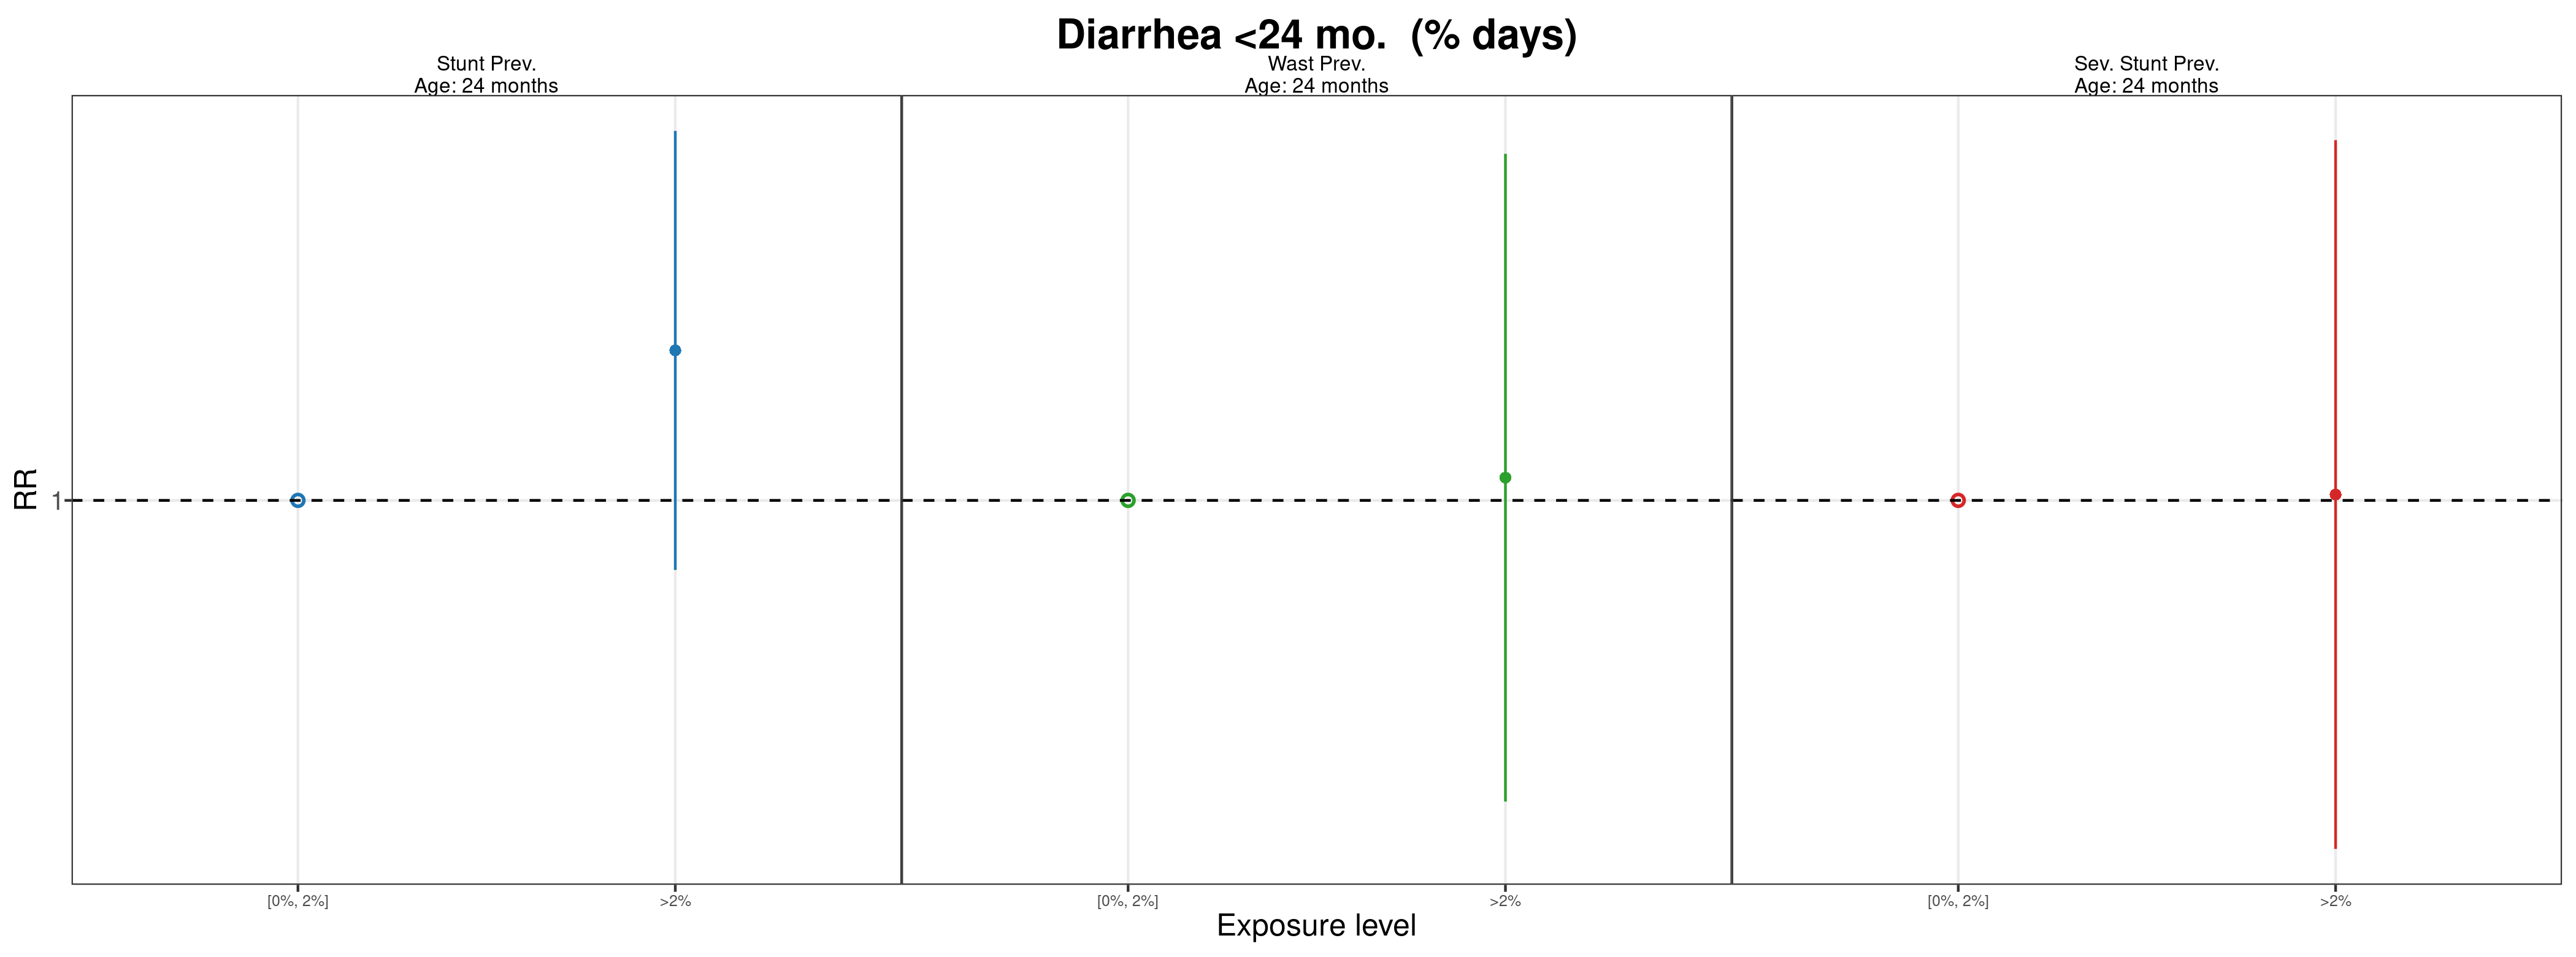
\includegraphics[width=58.33in]{C:/Users/andre/Documents/HBGDki/causes/ki-longitudinal-manuscripts/figures/risk-factor/RR-plots/fig-RR-perdiar24}
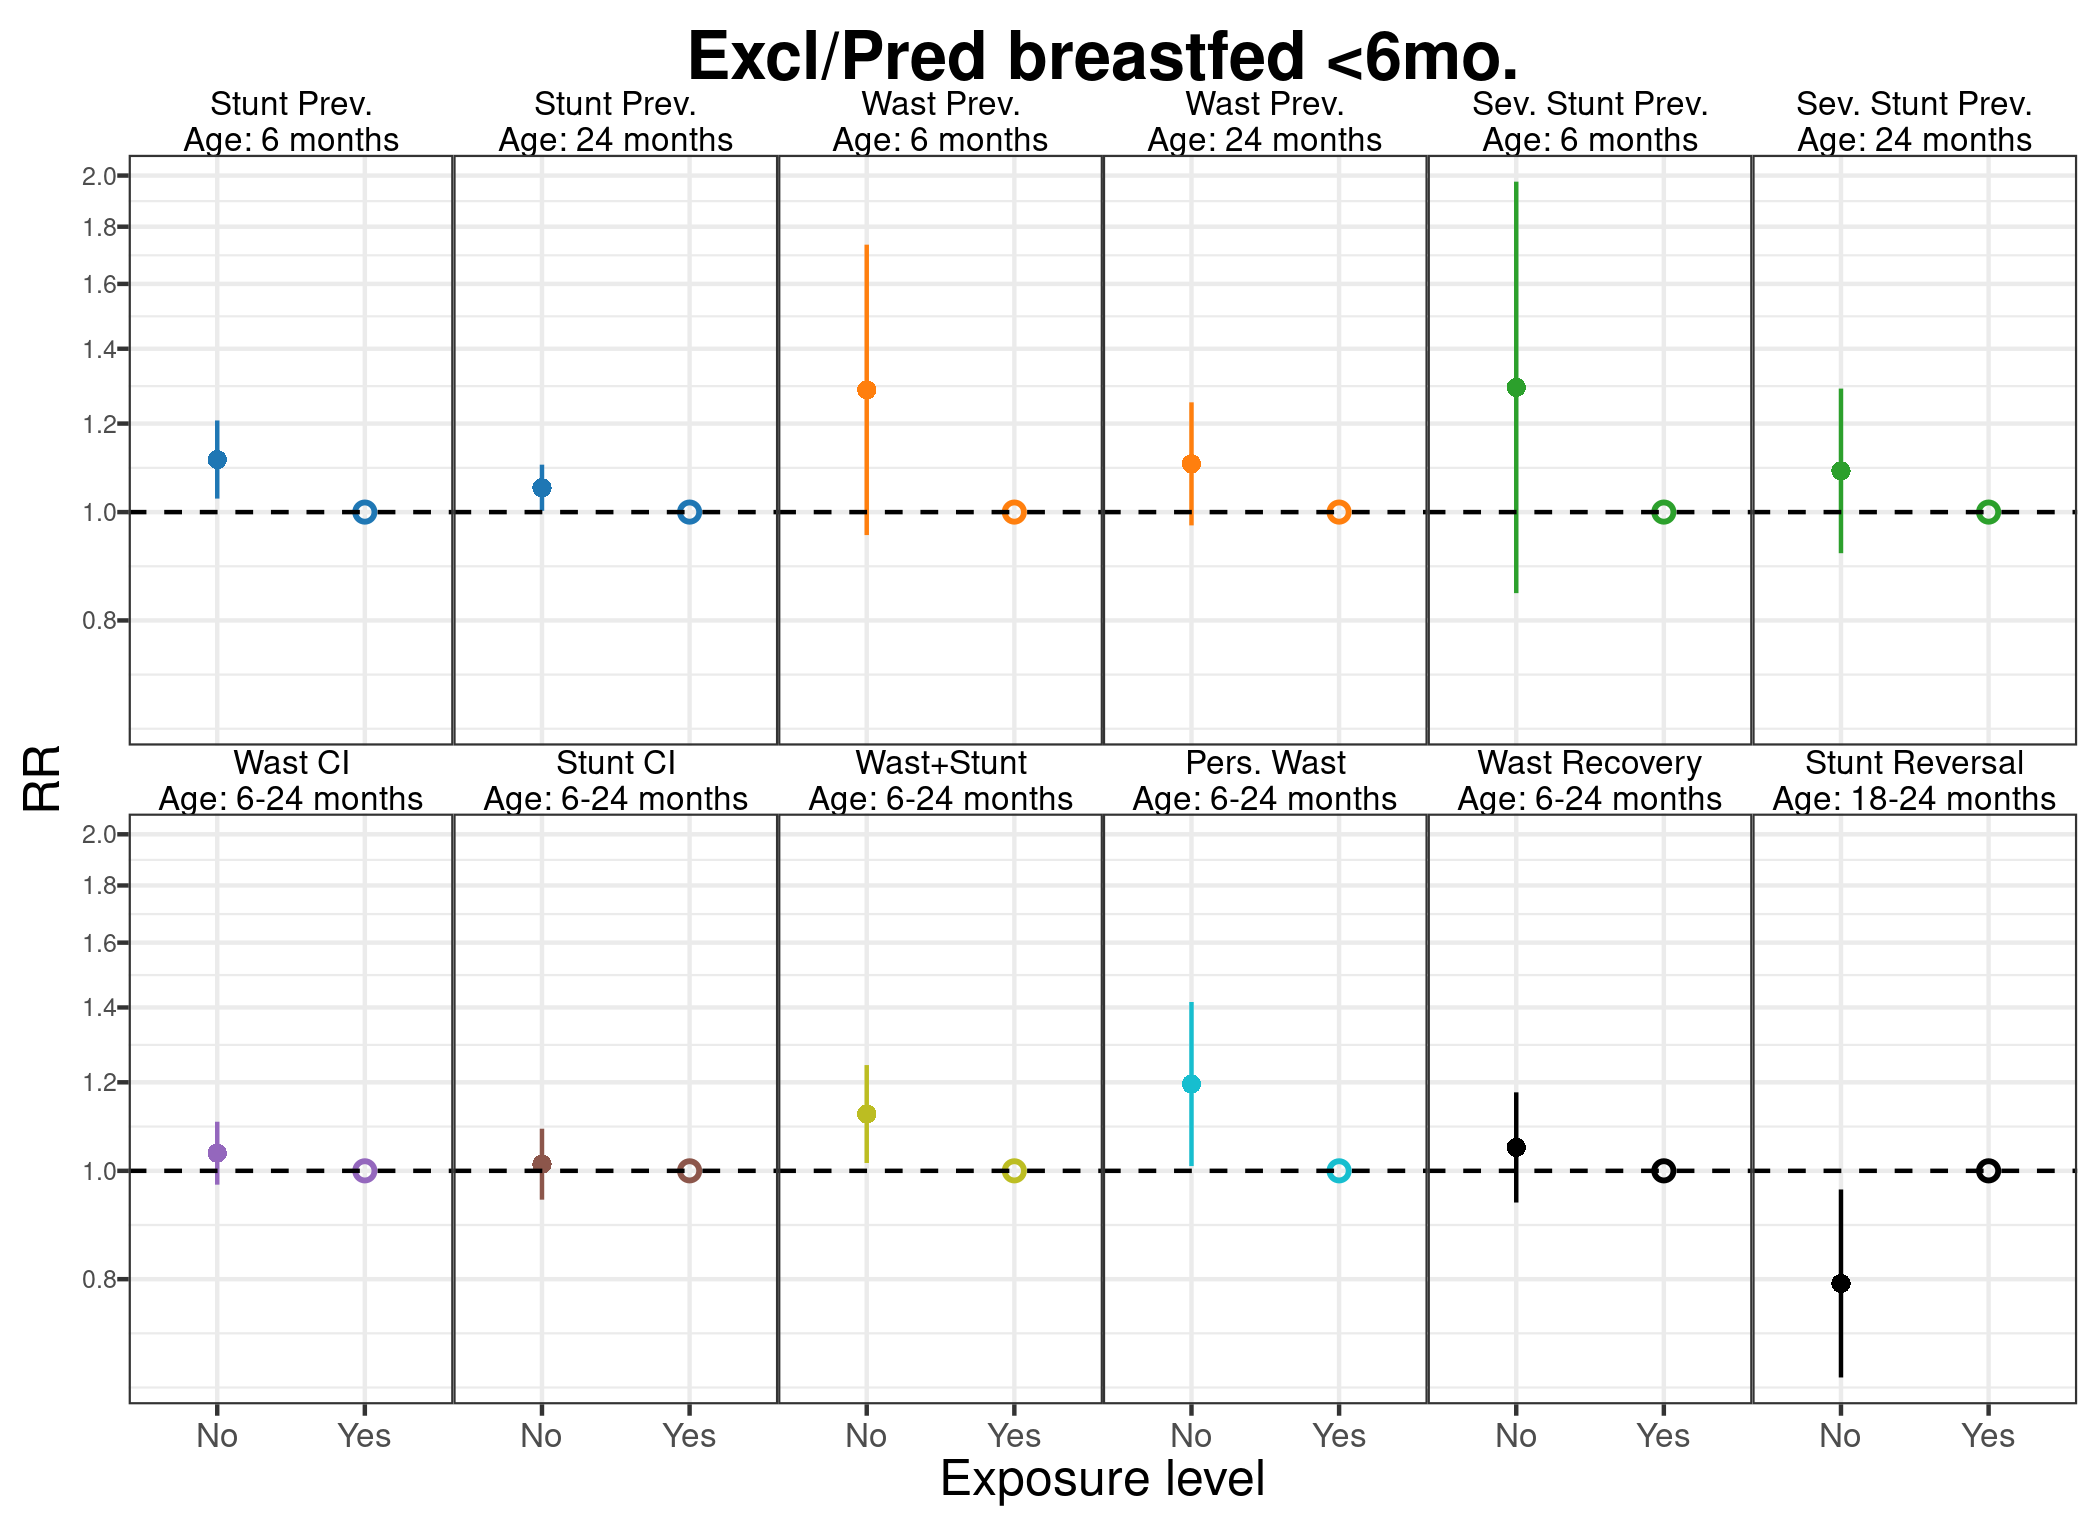
\includegraphics[width=58.33in]{C:/Users/andre/Documents/HBGDki/causes/ki-longitudinal-manuscripts/figures/risk-factor/RR-plots/fig-RR-predexfd6}
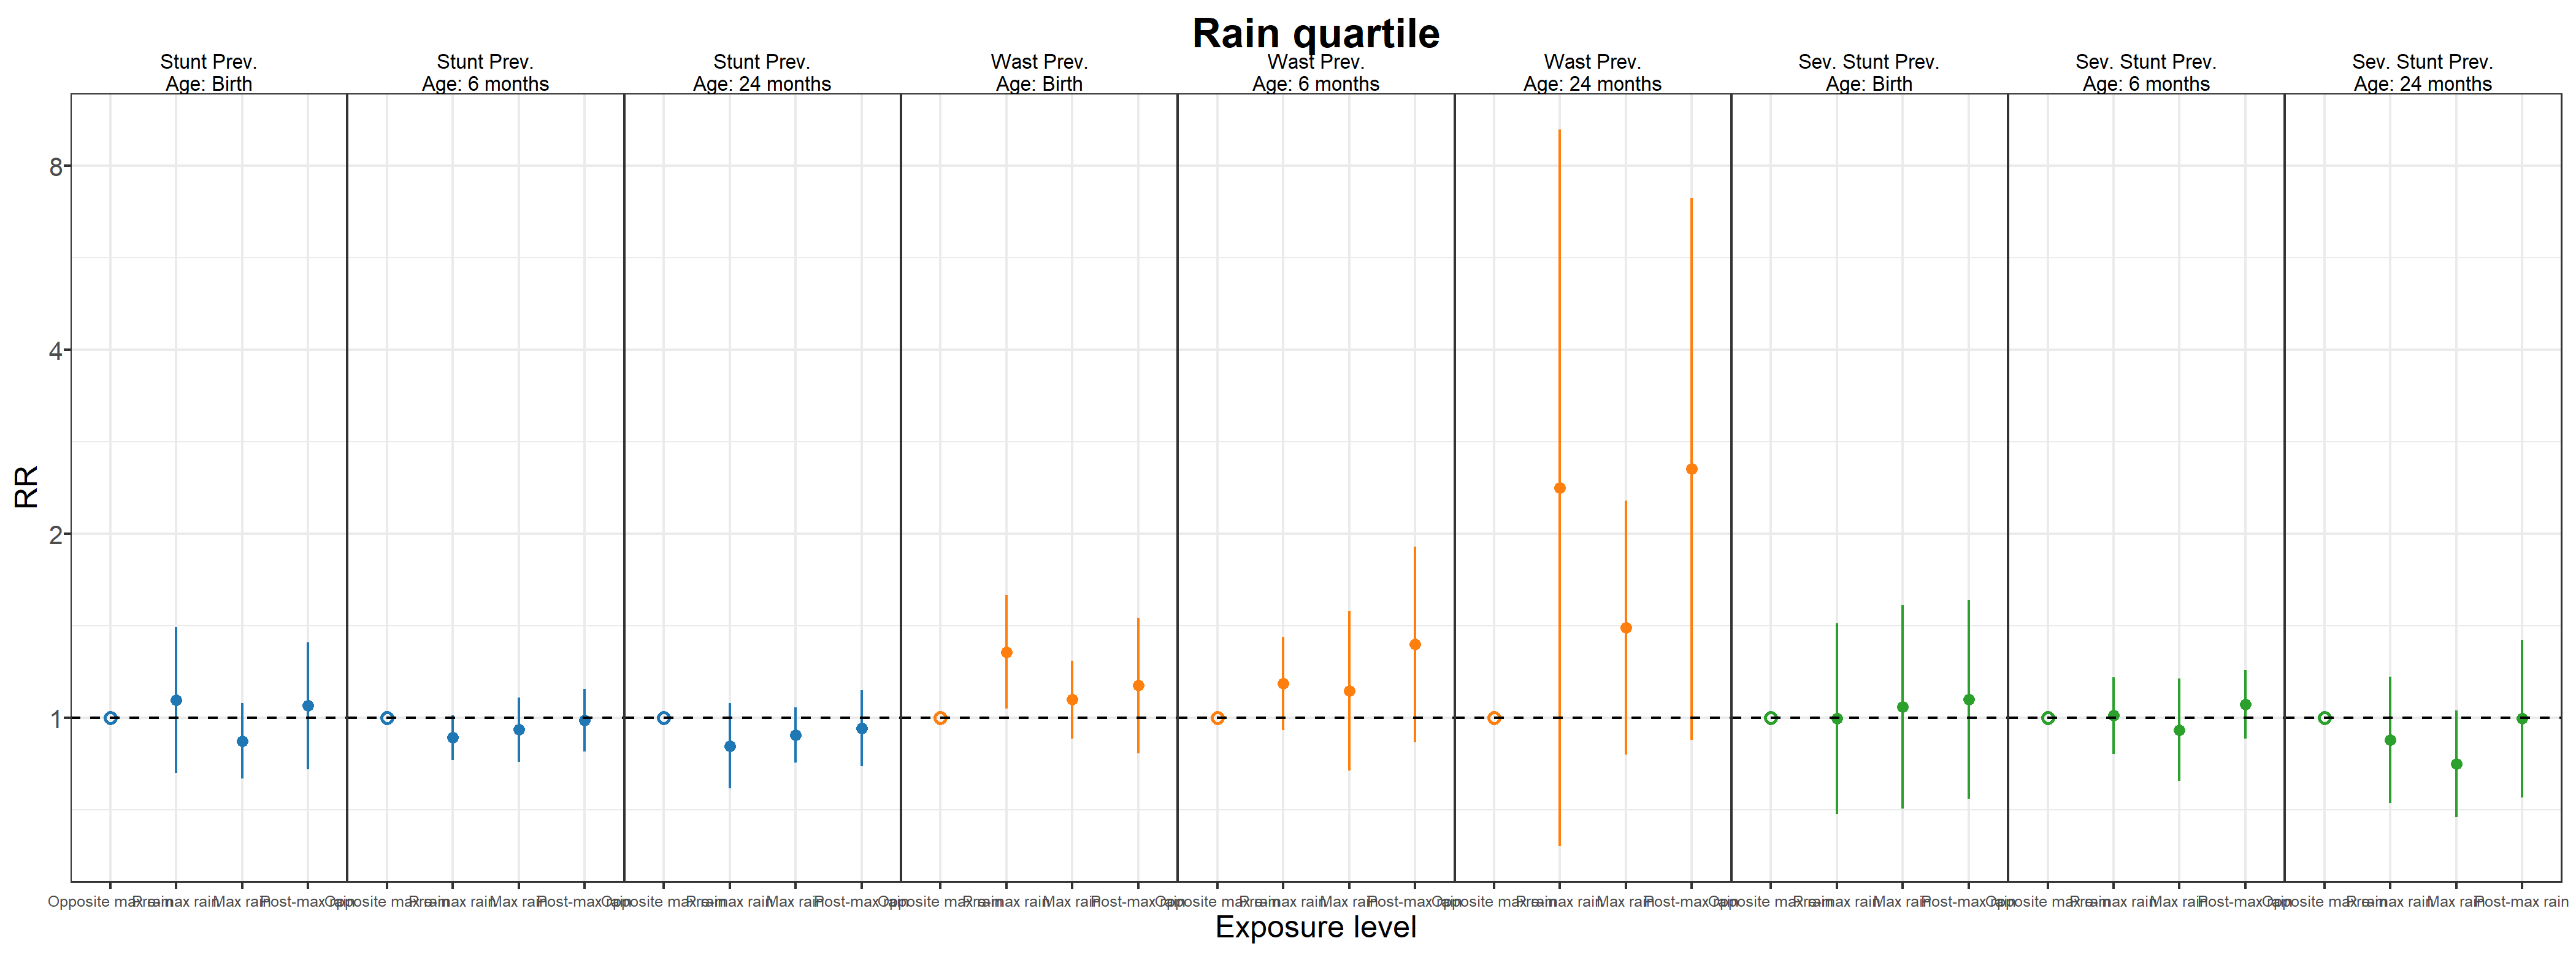
\includegraphics[width=58.33in]{C:/Users/andre/Documents/HBGDki/causes/ki-longitudinal-manuscripts/figures/risk-factor/RR-plots/fig-RR-rain_quartile}
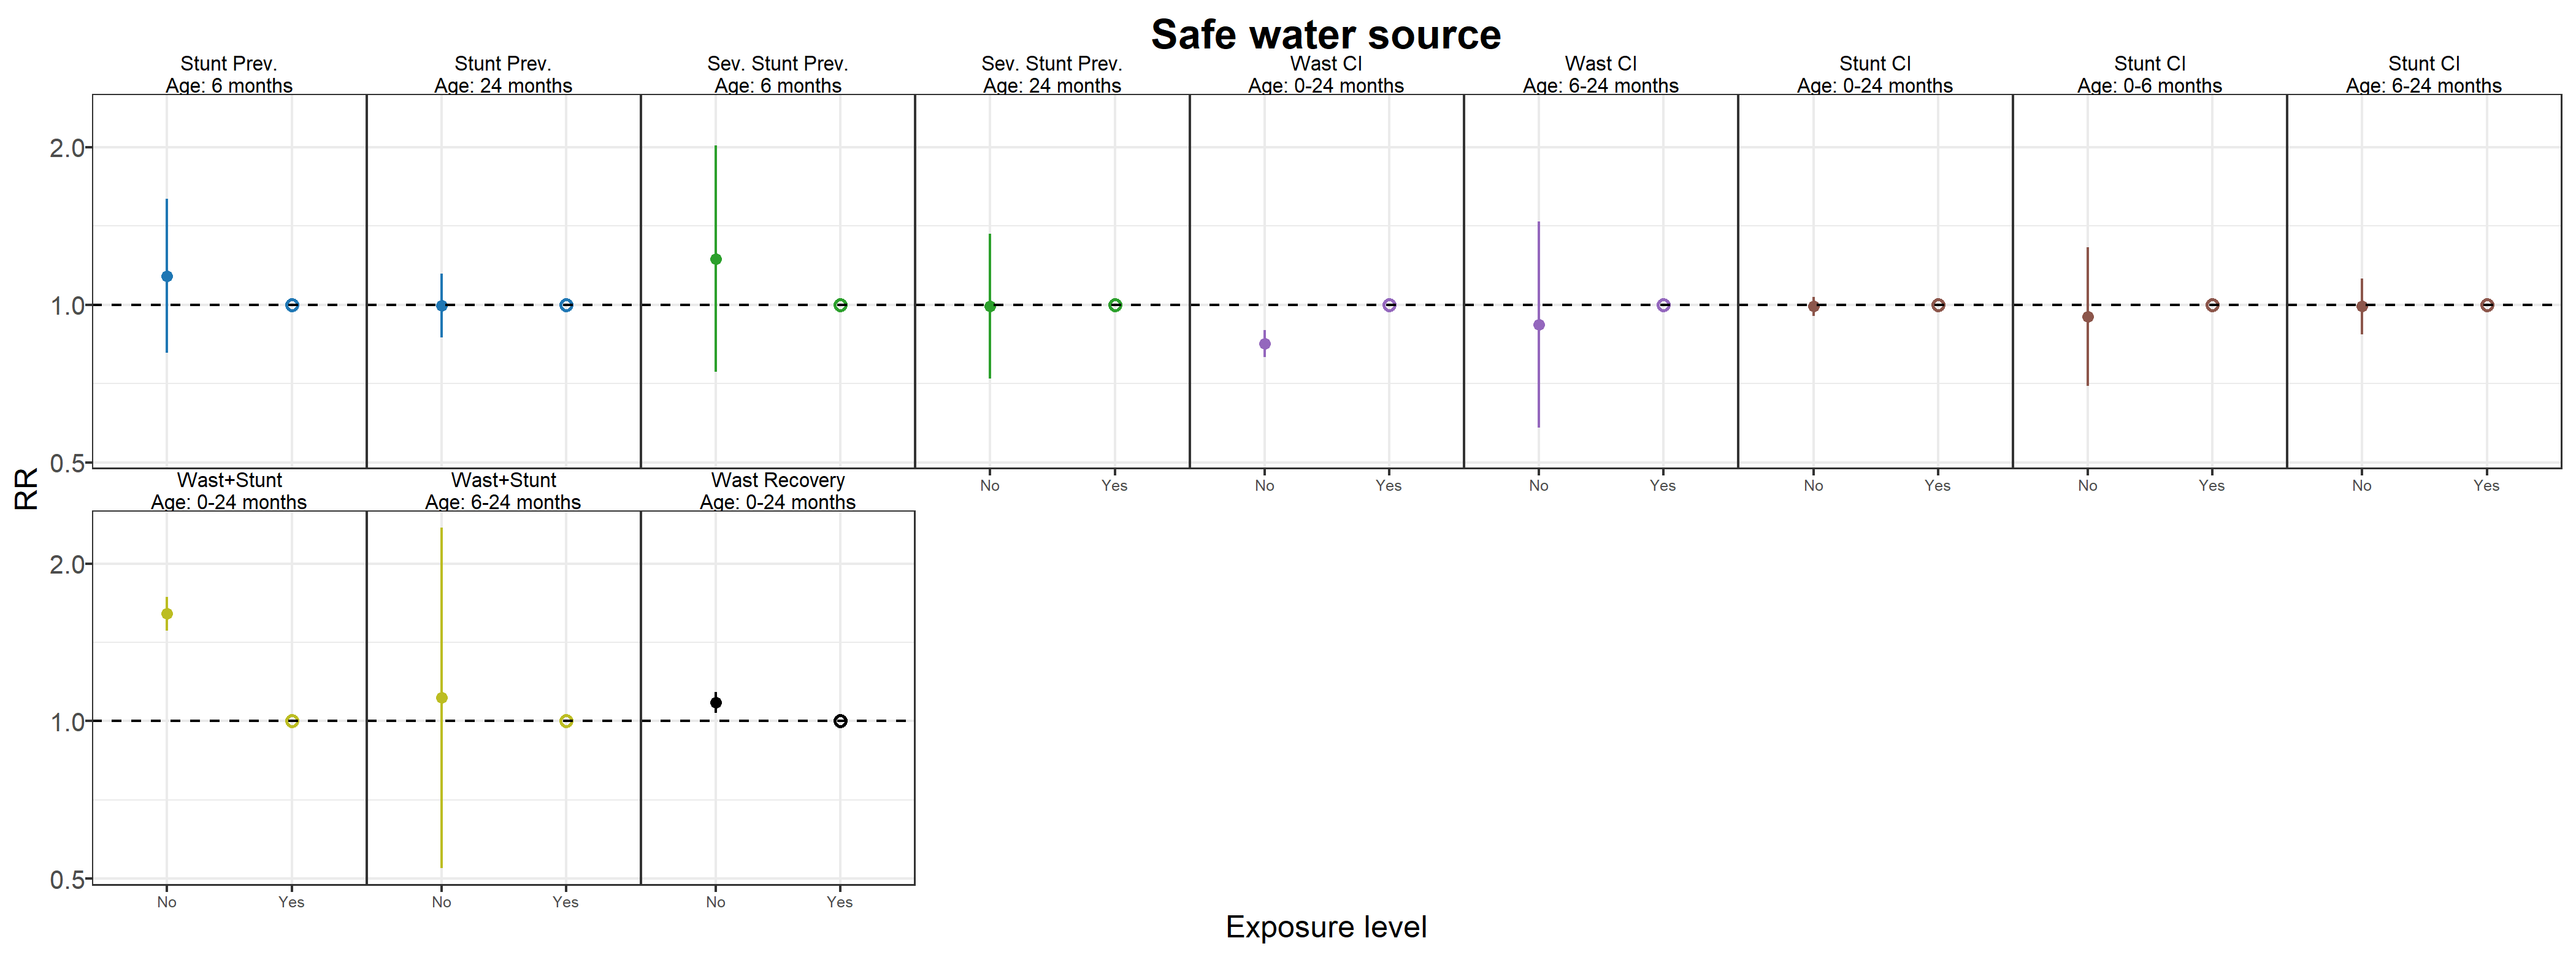
\includegraphics[width=58.33in]{C:/Users/andre/Documents/HBGDki/causes/ki-longitudinal-manuscripts/figures/risk-factor/RR-plots/fig-RR-safeh20}
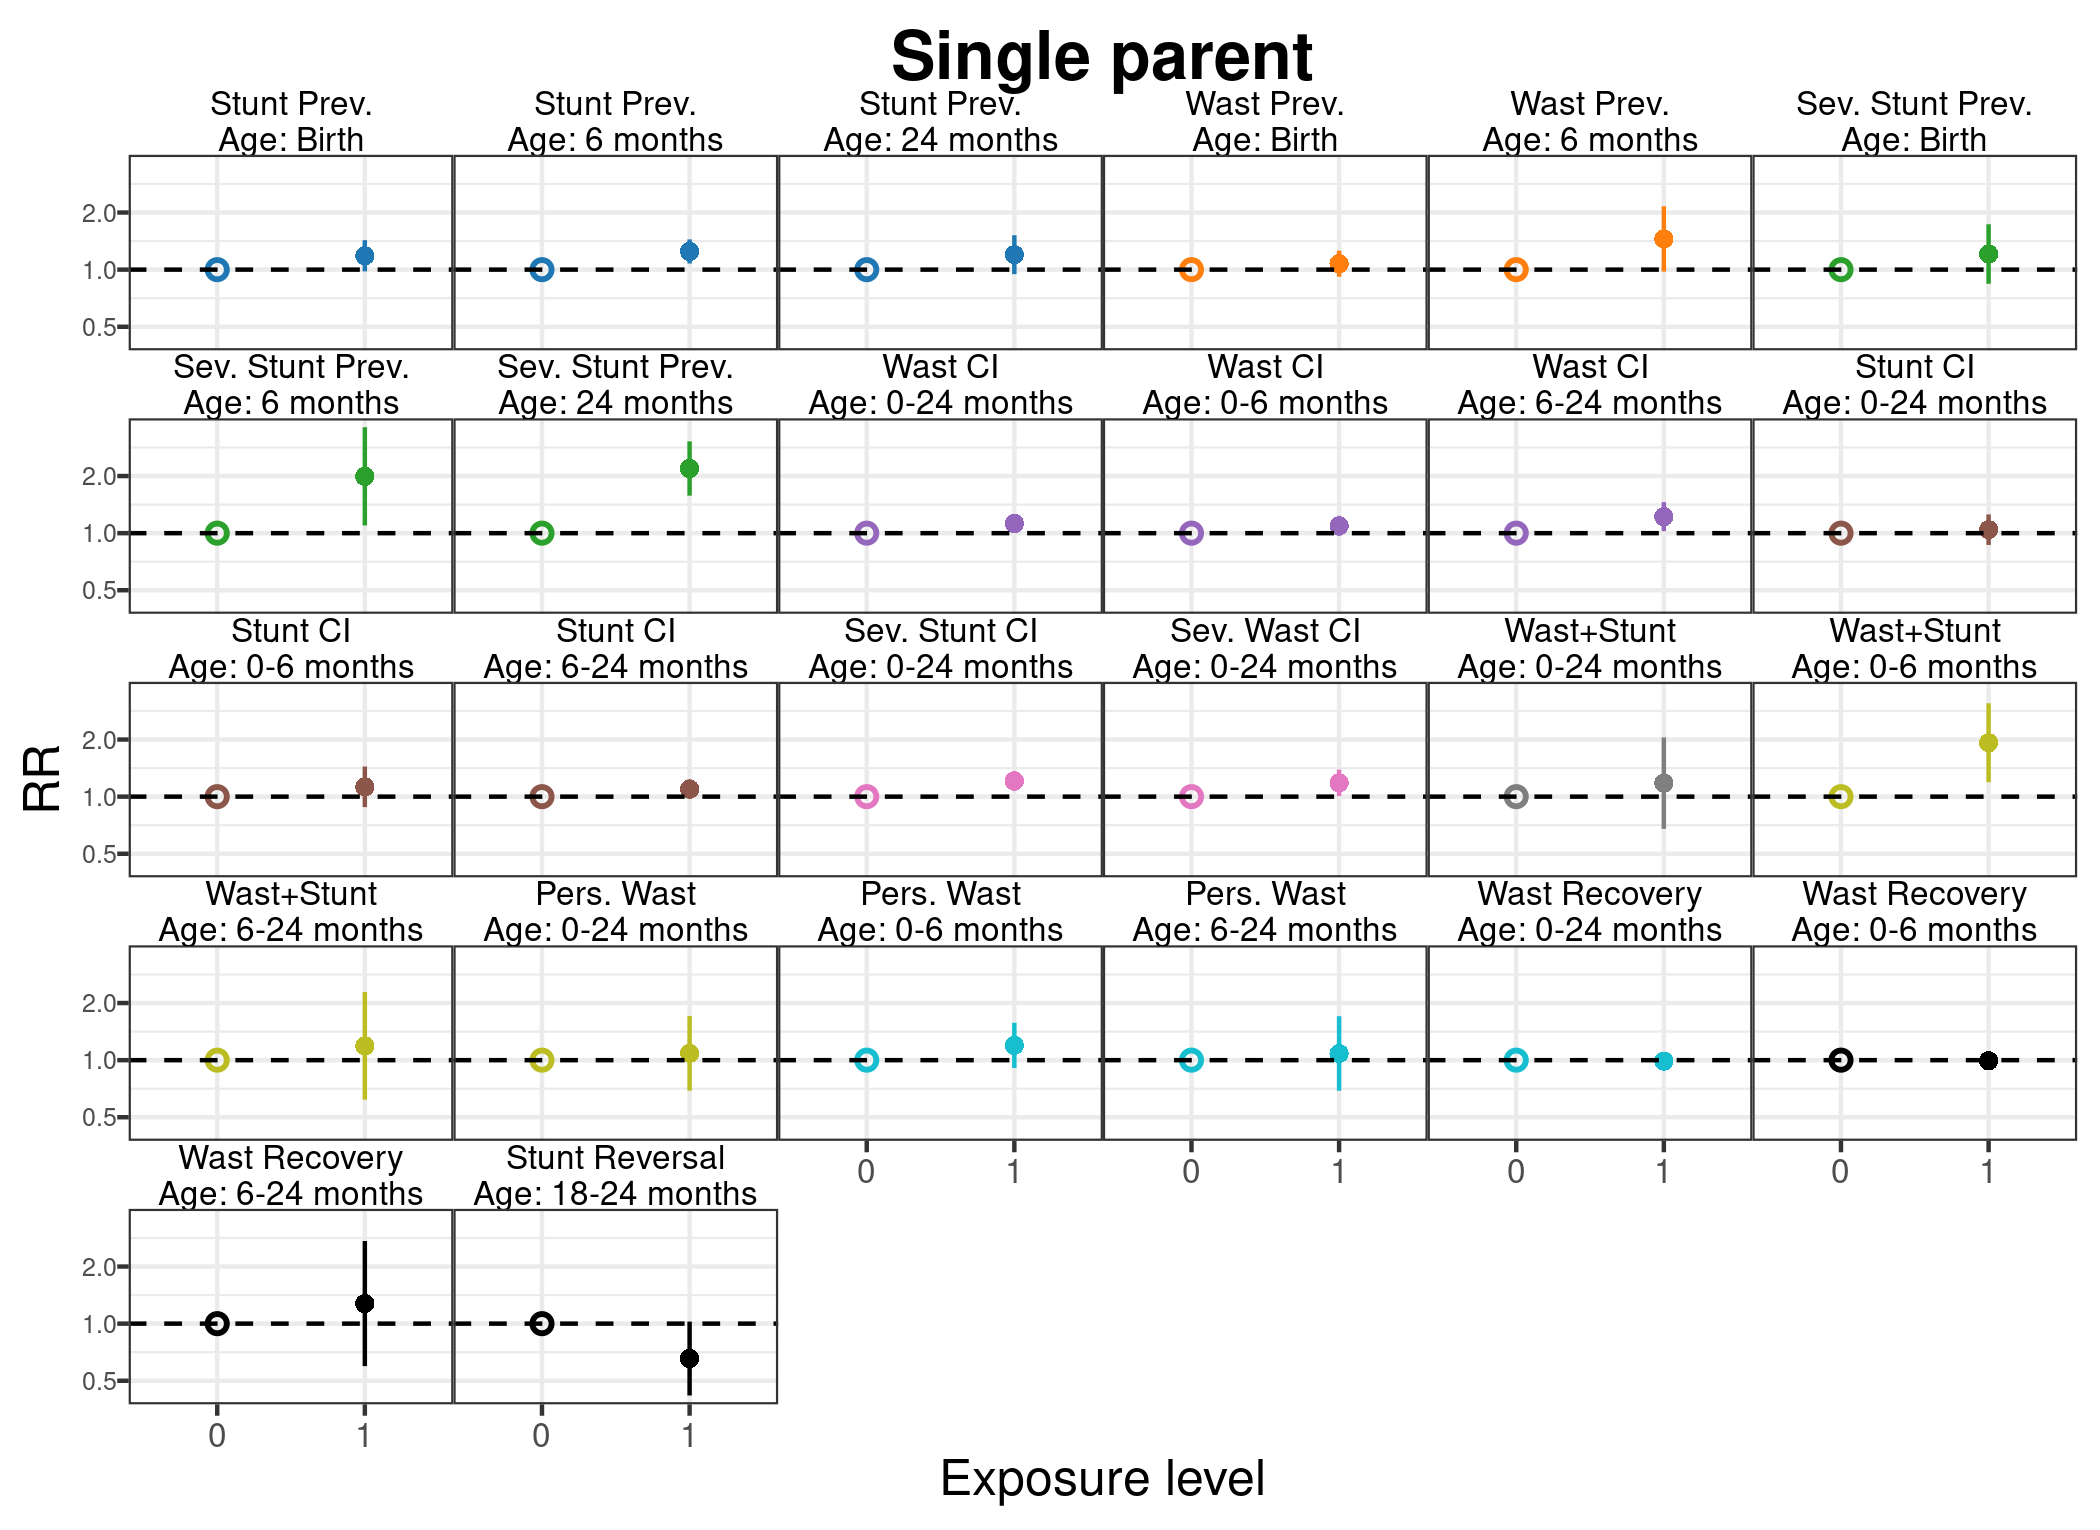
\includegraphics[width=58.33in]{C:/Users/andre/Documents/HBGDki/causes/ki-longitudinal-manuscripts/figures/risk-factor/RR-plots/fig-RR-single}
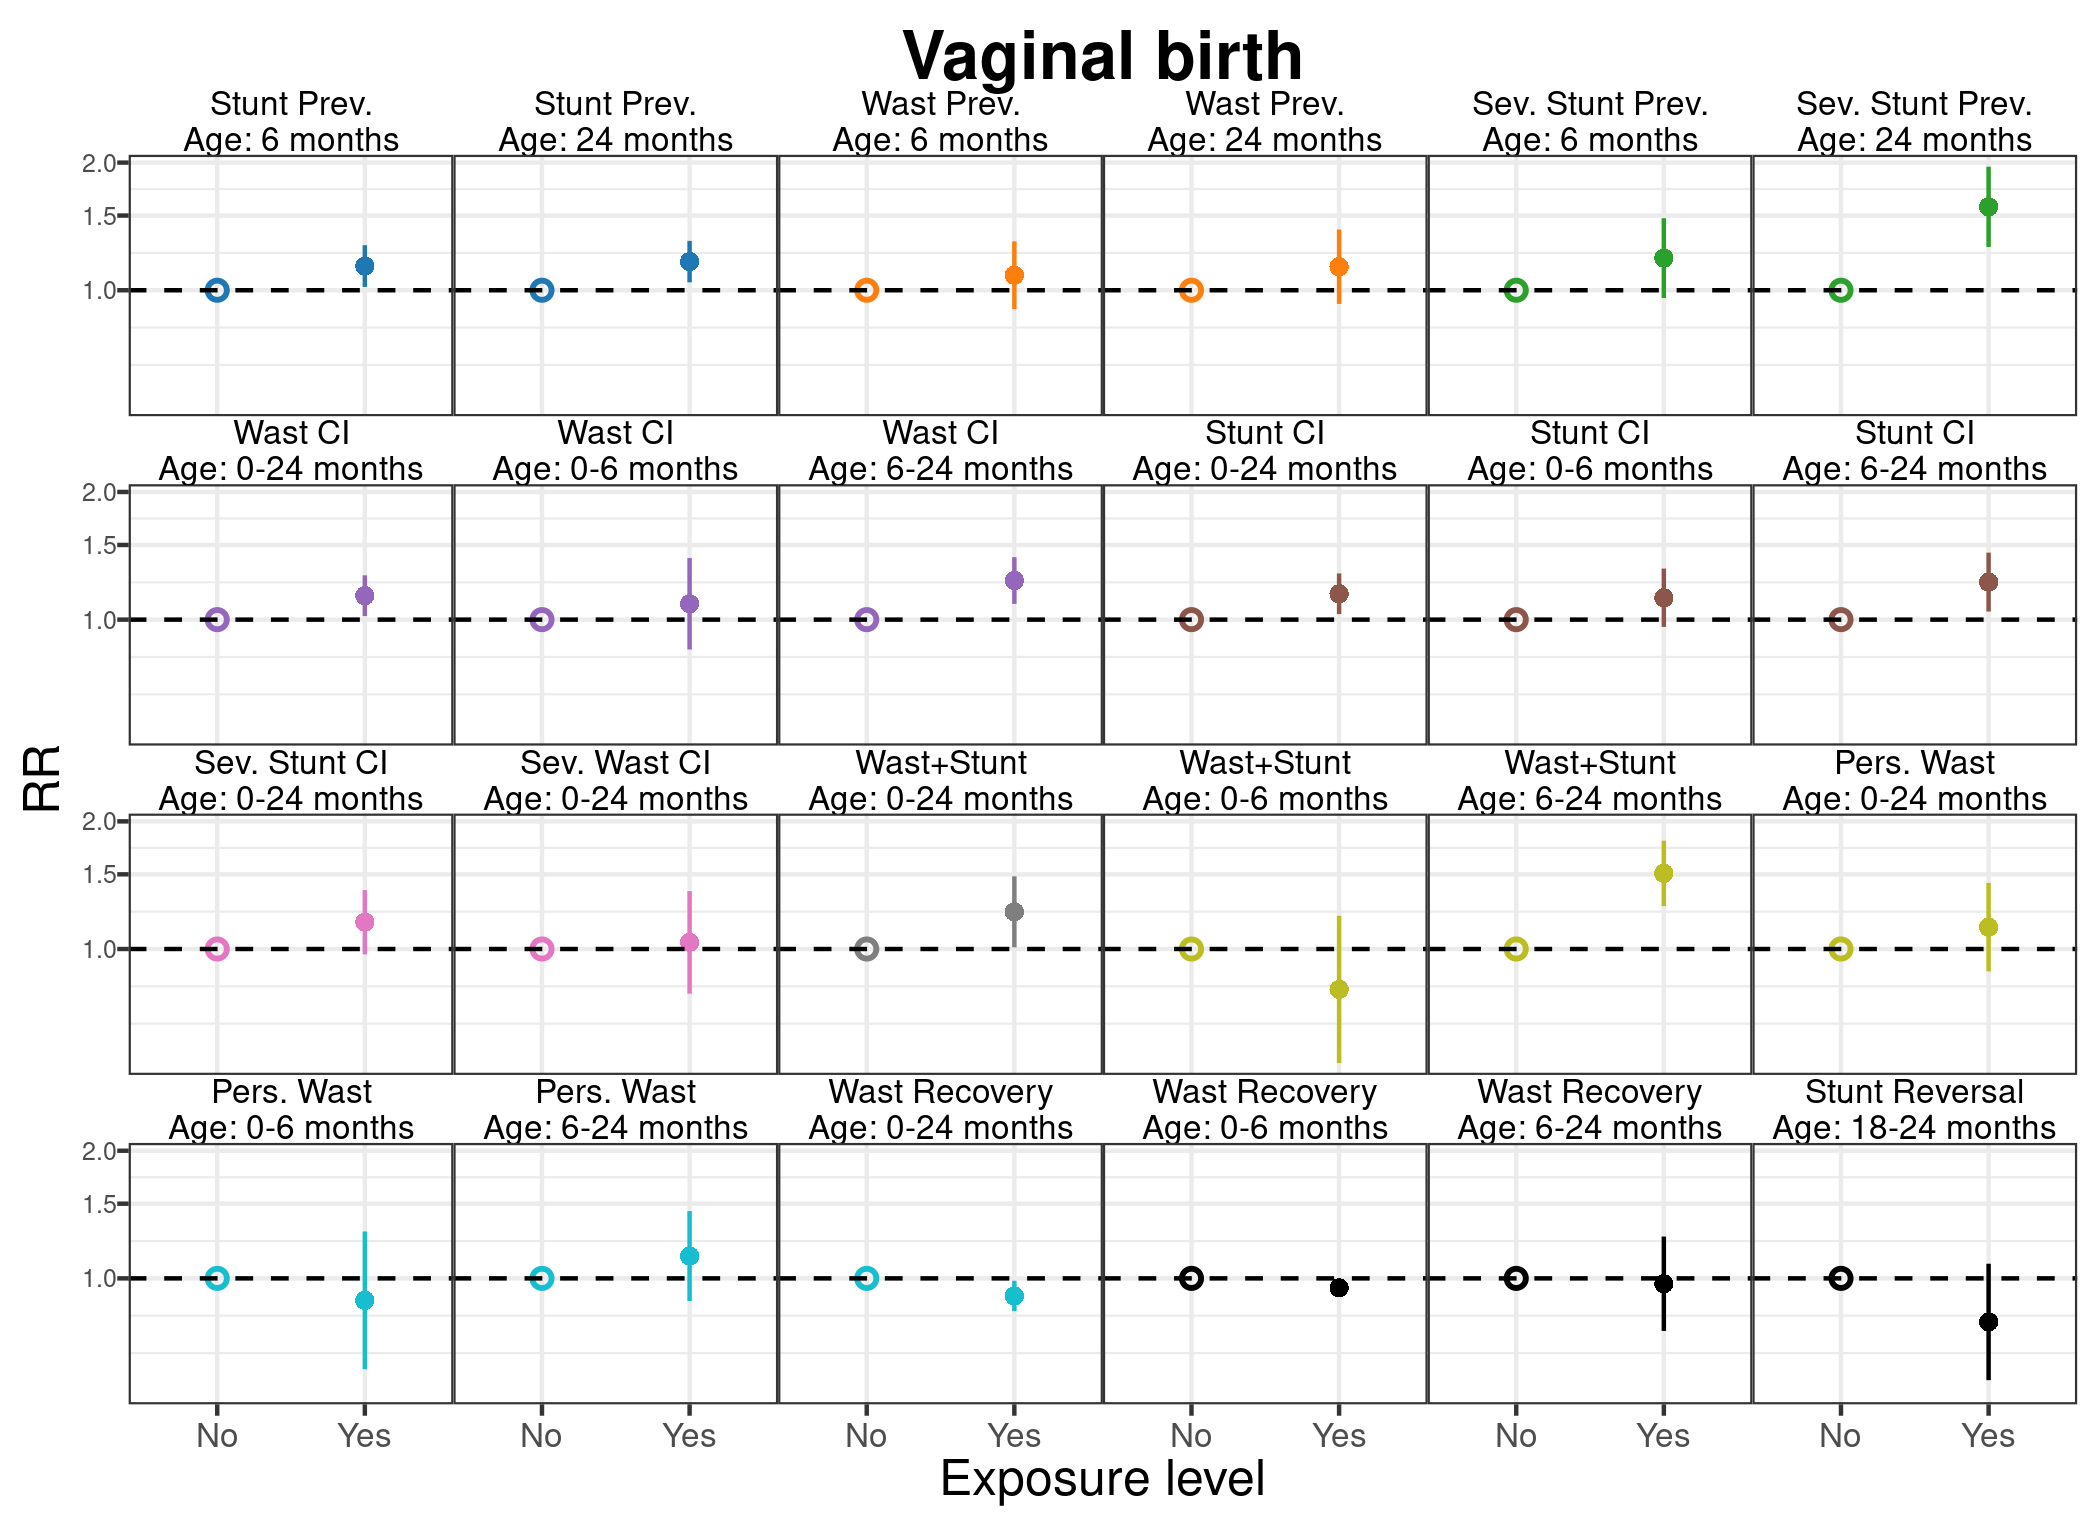
\includegraphics[width=58.33in]{C:/Users/andre/Documents/HBGDki/causes/ki-longitudinal-manuscripts/figures/risk-factor/RR-plots/fig-RR-vagbrth}

\hypertarget{velocity}{%
\chapter{Growth velocity}\label{velocity}}

\raggedright

** {[}Coming soon{]} Will fill in with PAR plots of growth velocity **

\hypertarget{fixed-effects}{%
\chapter{Sensitivity analysis using fixed effects}\label{fixed-effects}}

\raggedright

The primary analyses presented in this manuscript pooled across individual studies using random effects. Inferences about estimates from fixed effects models are restricted to only the included studies.{[}\^{}1{]} The random effects approach was more conservative in the presence of study heterogeneity, as evidenced by larger confidence intervals around each point estimates. Overall, the inference from results produced by each method was similar.

\hypertarget{primary-manuscript-figures-recreated-with-estimates-pooled-using-fixed-effects}{%
\section{Primary manuscript figures recreated with estimates pooled using fixed effects}\label{primary-manuscript-figures-recreated-with-estimates-pooled-using-fixed-effects}}

More estimates are significant when pooling using fixed effects due to the generally smaller confidence intervals.

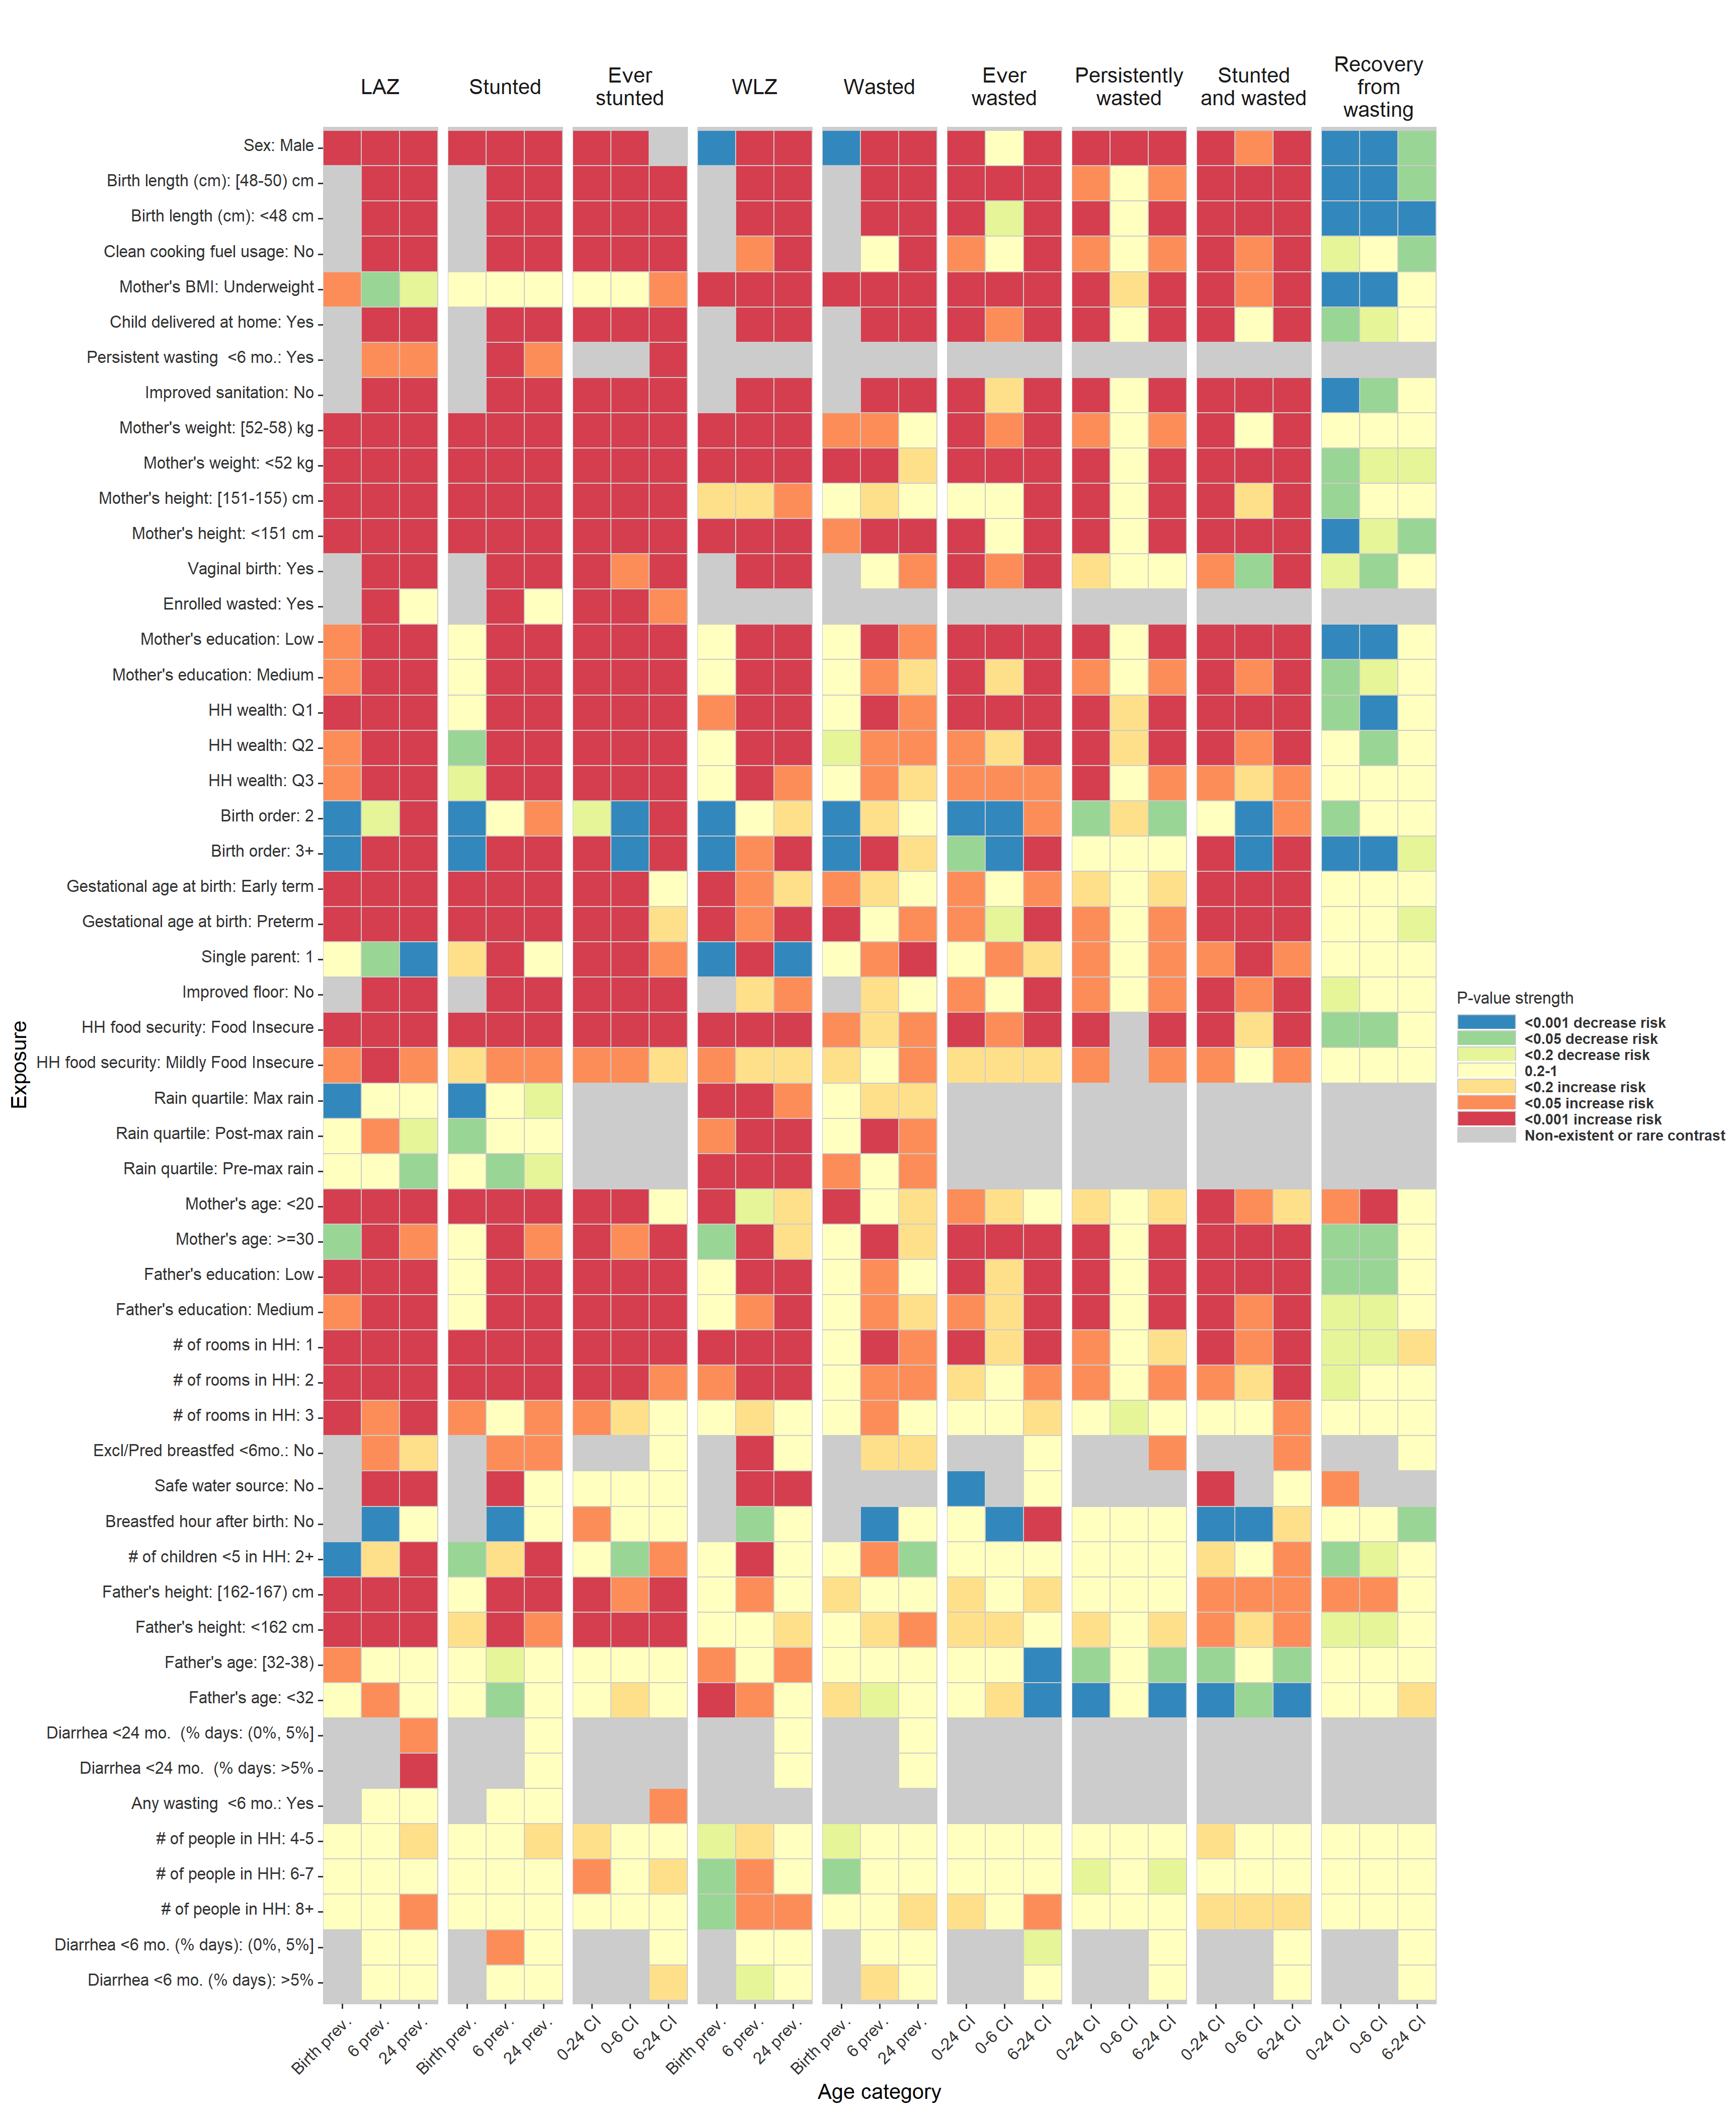
\includegraphics[width=47.92in]{C:/Users/andre/Documents/HBGDki/causes/ki-longitudinal-manuscripts/figures/risk-factor/fig-sig-heatmap_FE}
\textbf{Figure 1a. Heatmap of significance and direction across exposure-outcome combinations of associations estimated using fixed effects. }

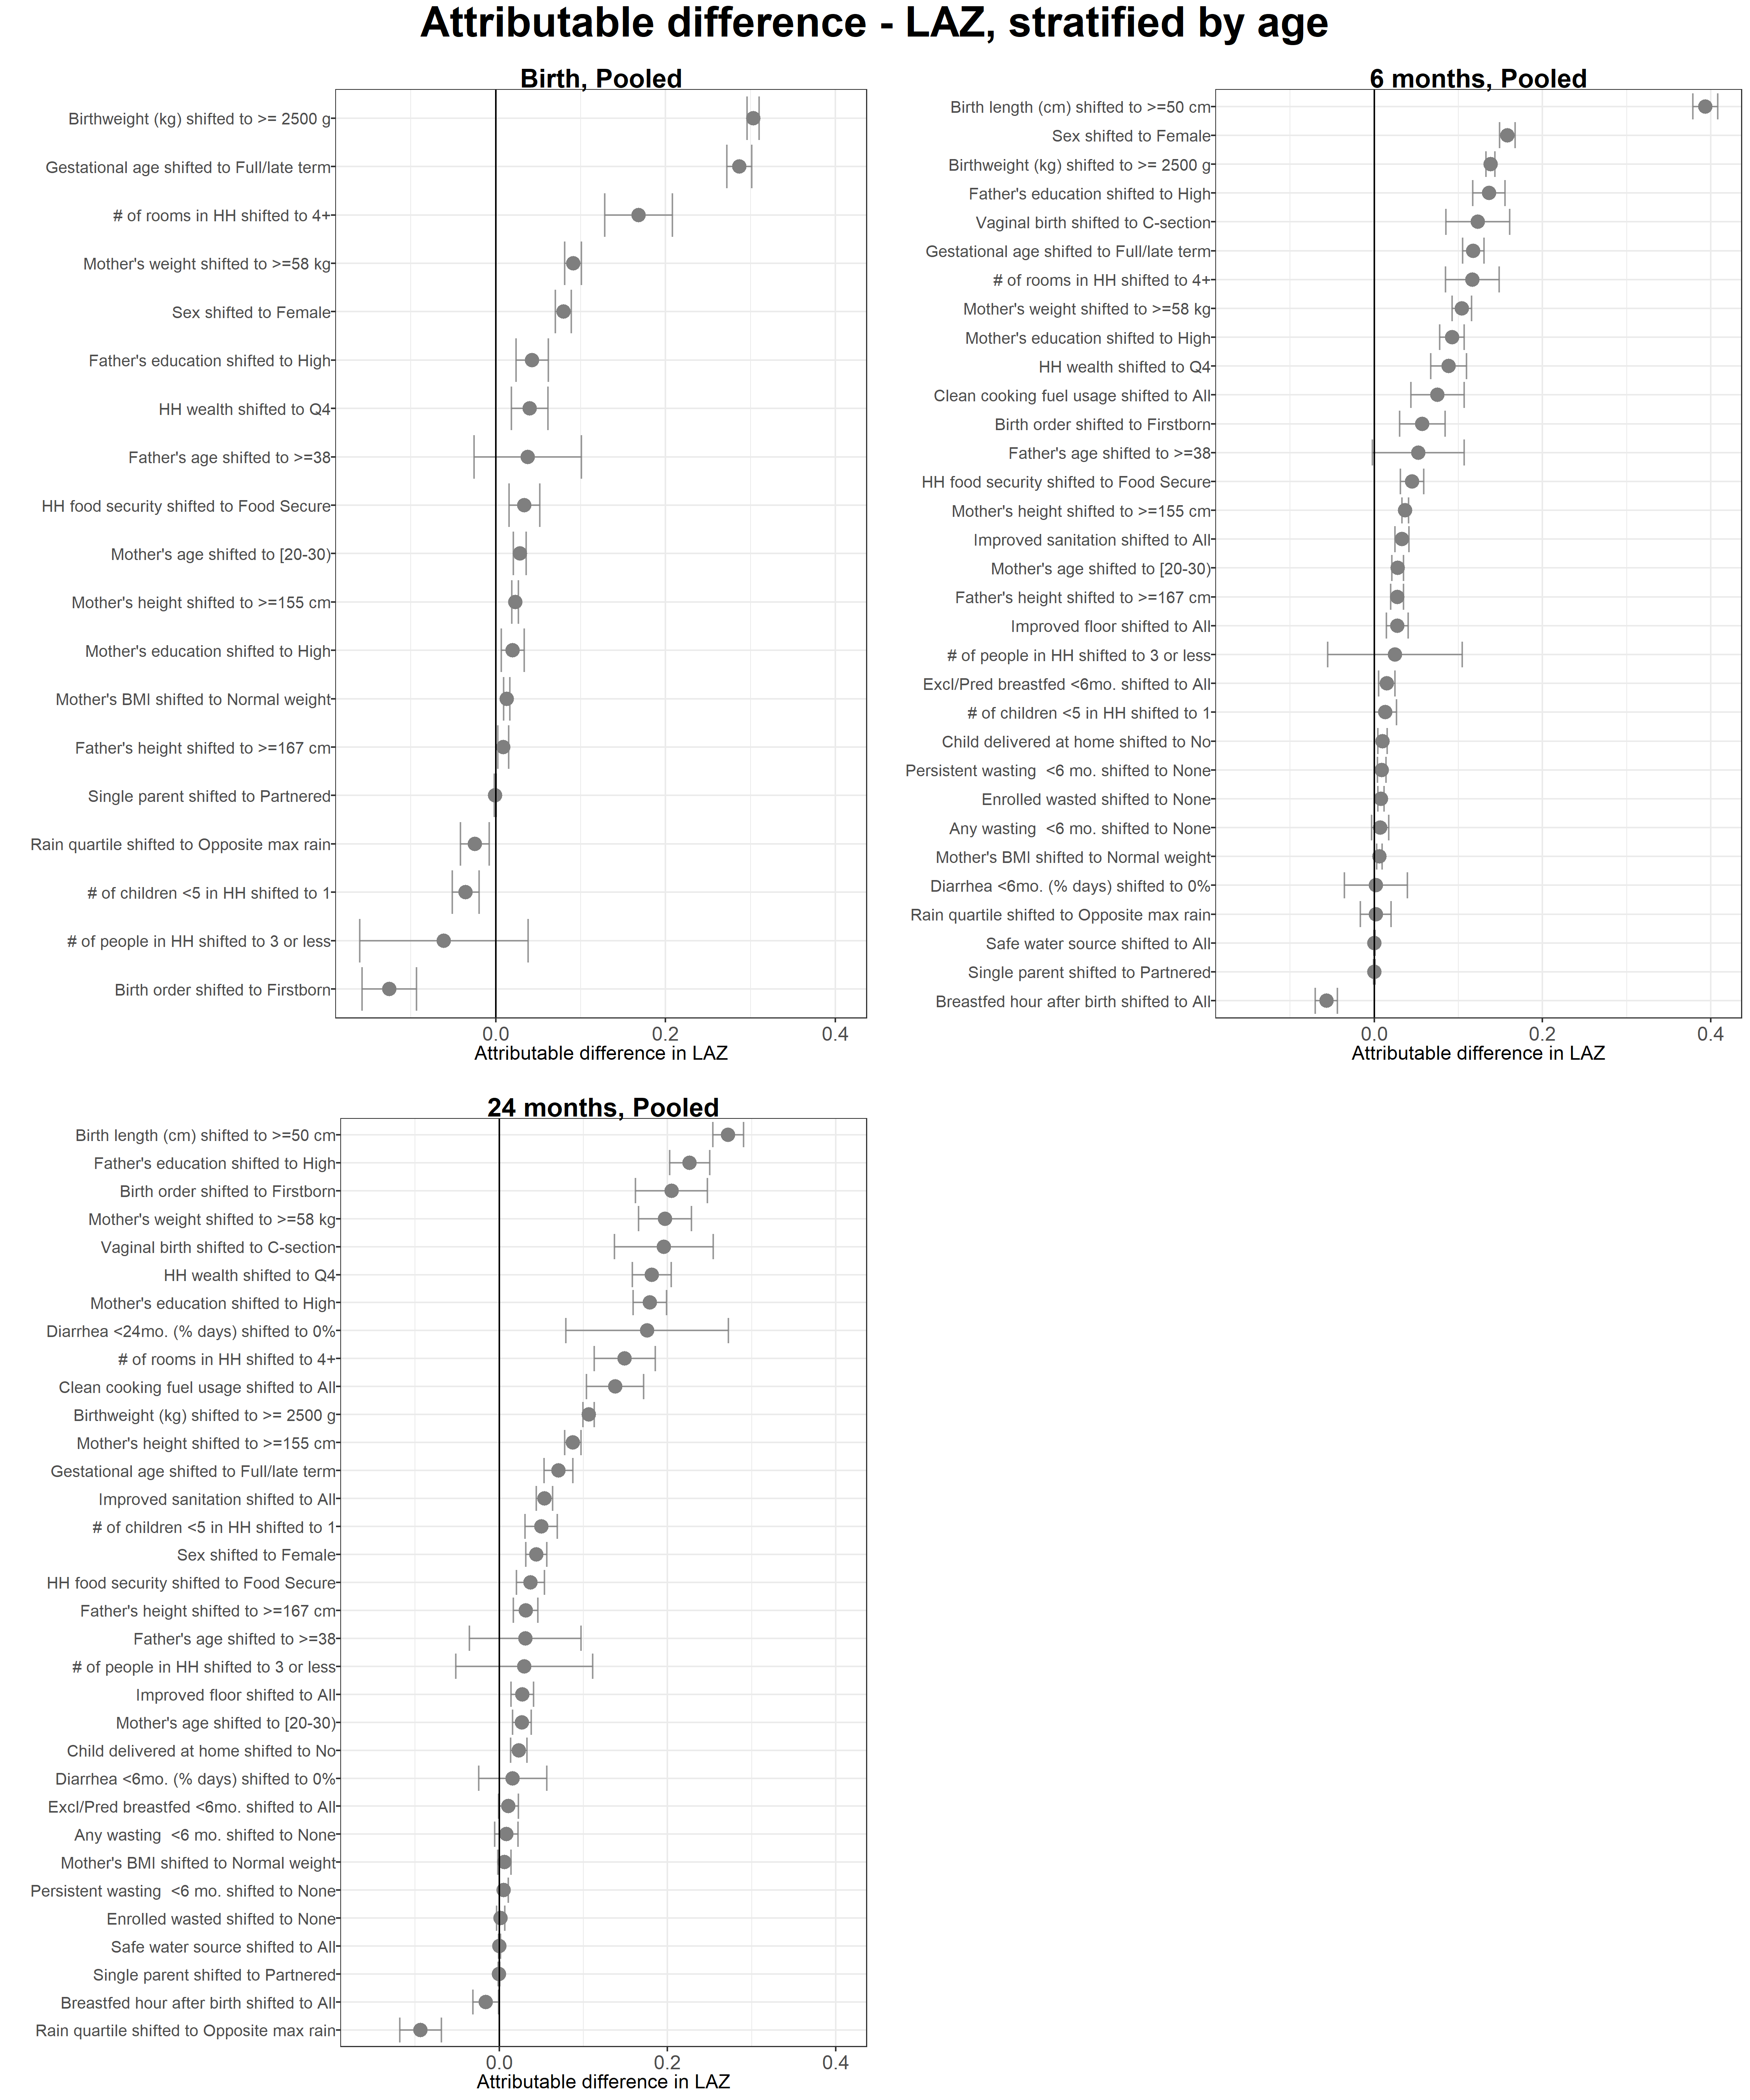
\includegraphics[width=62.5in]{C:/Users/andre/Documents/HBGDki/causes/ki-longitudinal-manuscripts/figures/manuscript-figure-composites/risk-factor/extended-data/fig-laz-PAR-strat-age_FE}
\textbf{Extended Data Figure 3 \textbar{} Age-stratified population attributable differences in length-for-age Z-scores estimated using fixed effects. }

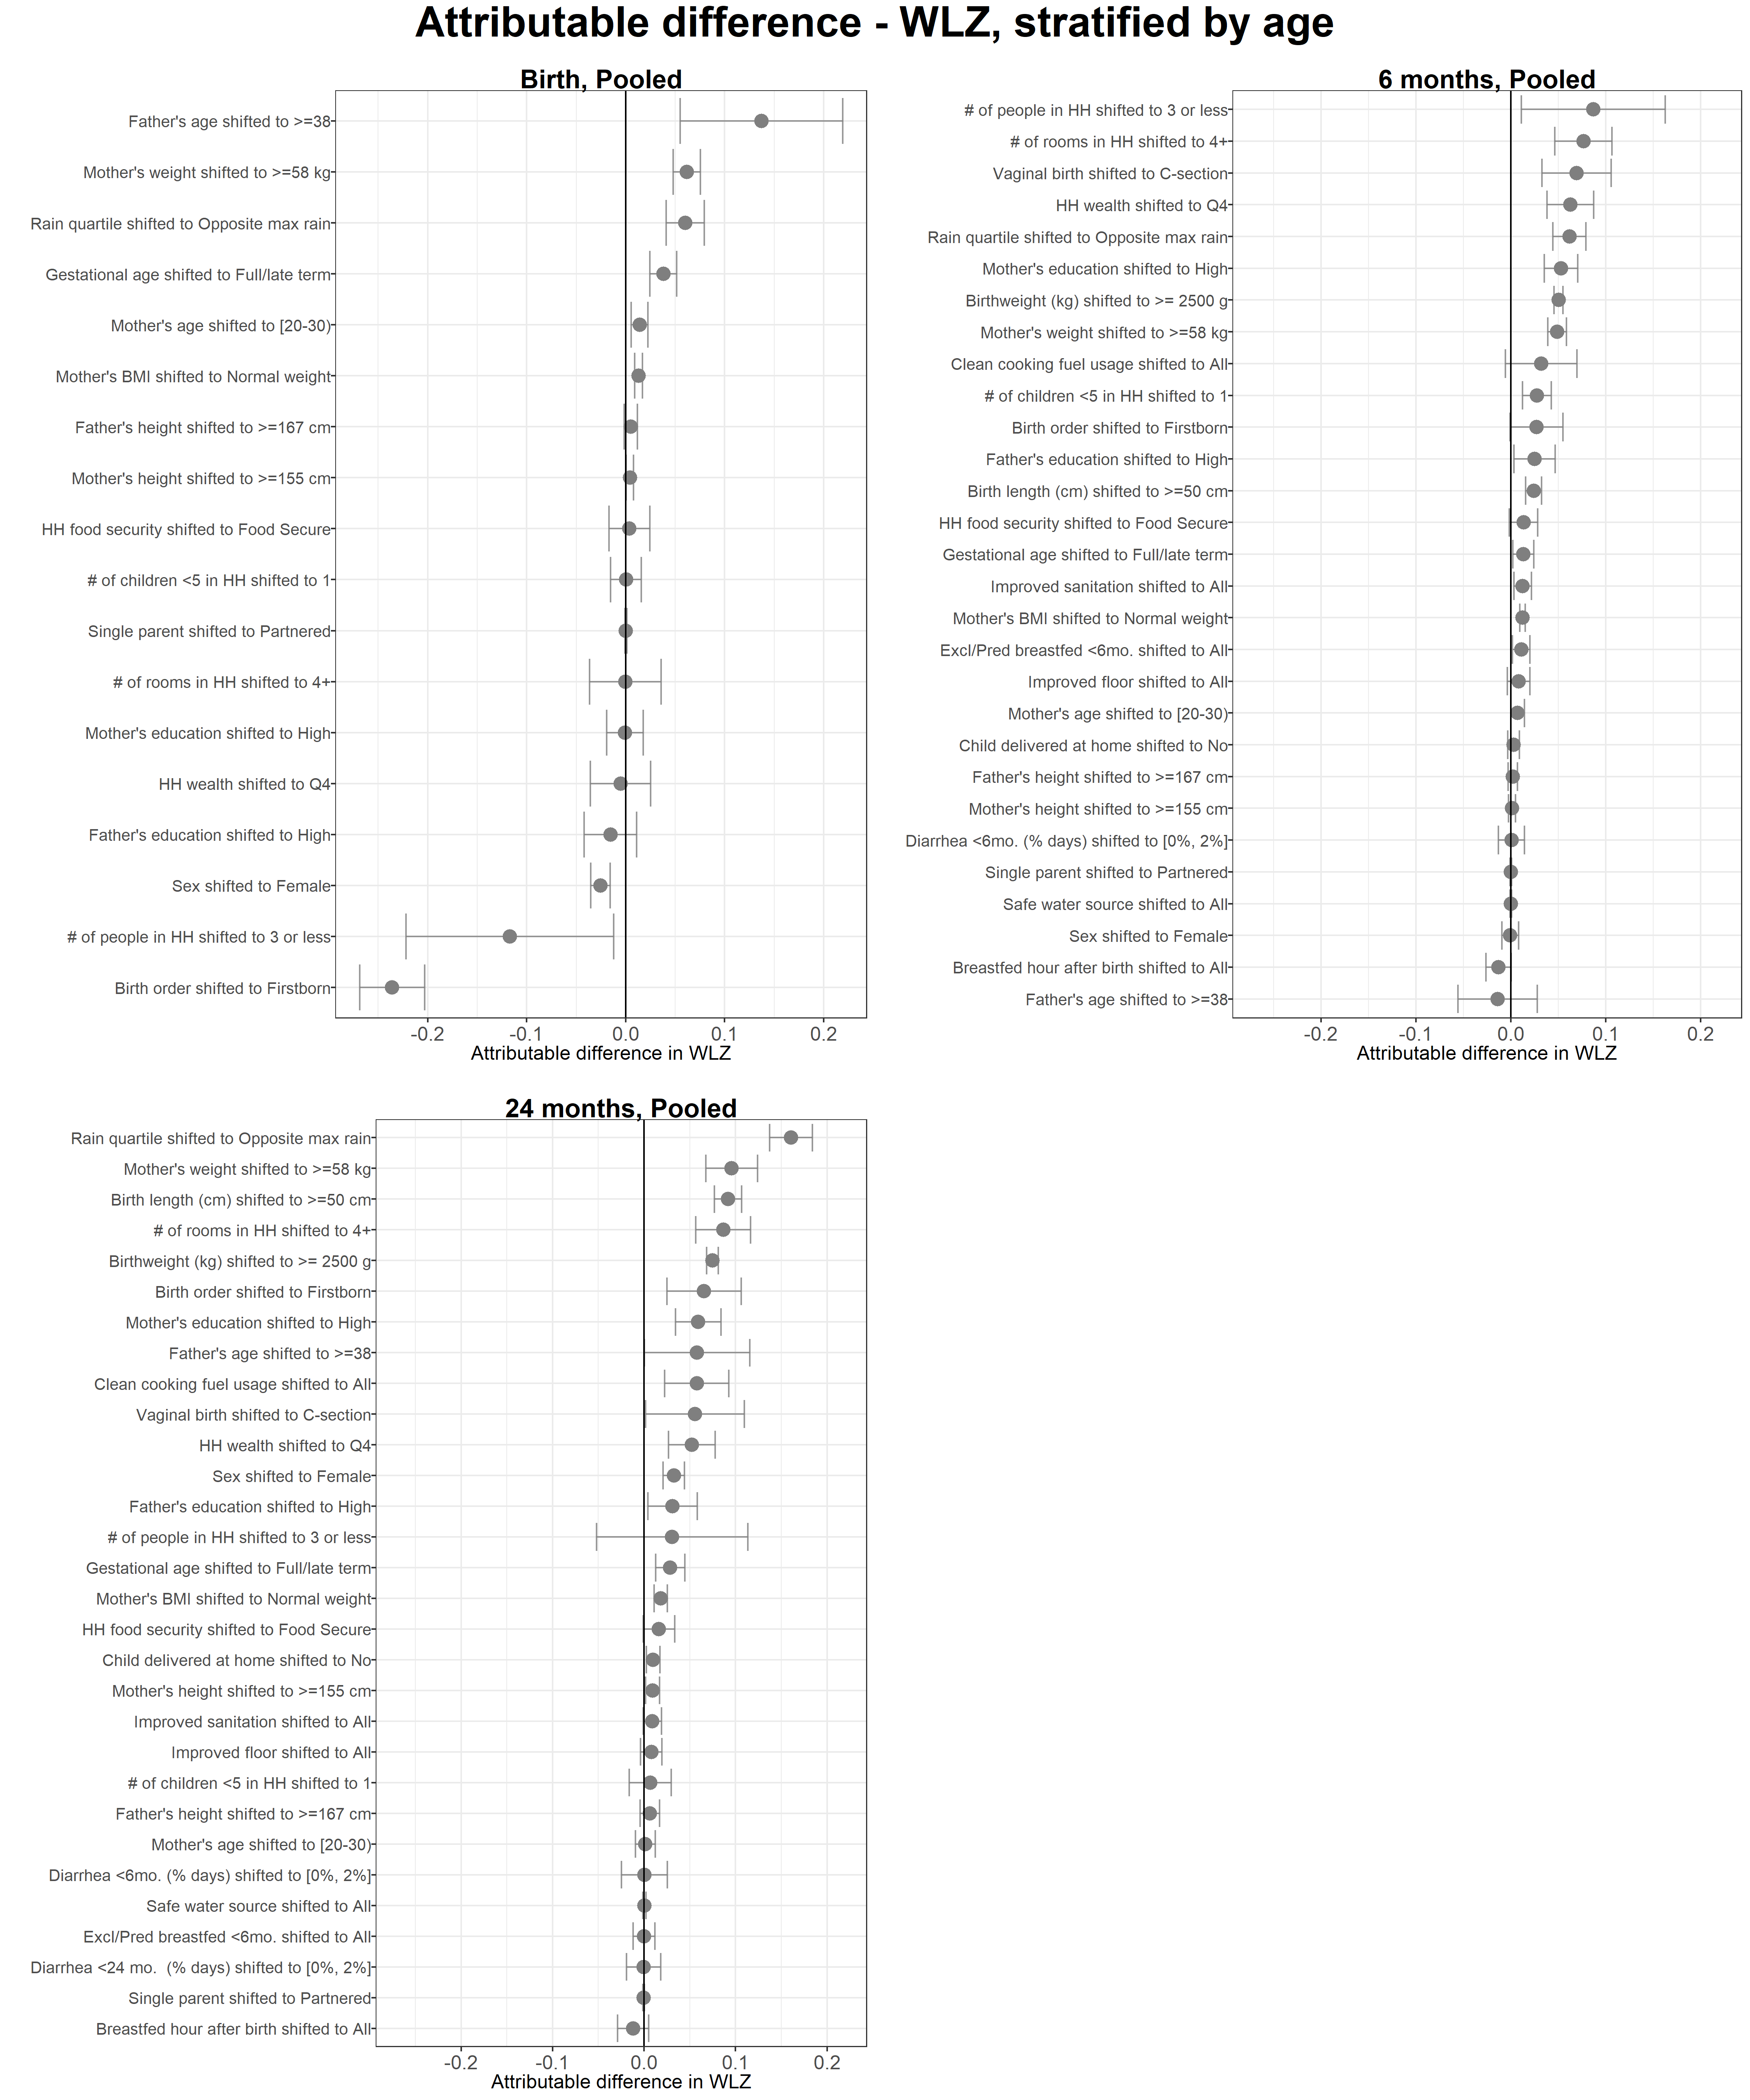
\includegraphics[width=62.5in]{C:/Users/andre/Documents/HBGDki/causes/ki-longitudinal-manuscripts/figures/manuscript-figure-composites/risk-factor/extended-data/fig-wlz-PAR-strat-age_FE}
\textbf{Extended Data Figure 4 \textbar{} Age-stratified population attributable differences in weight-for-length Z-scores estimated using fixed effects. }

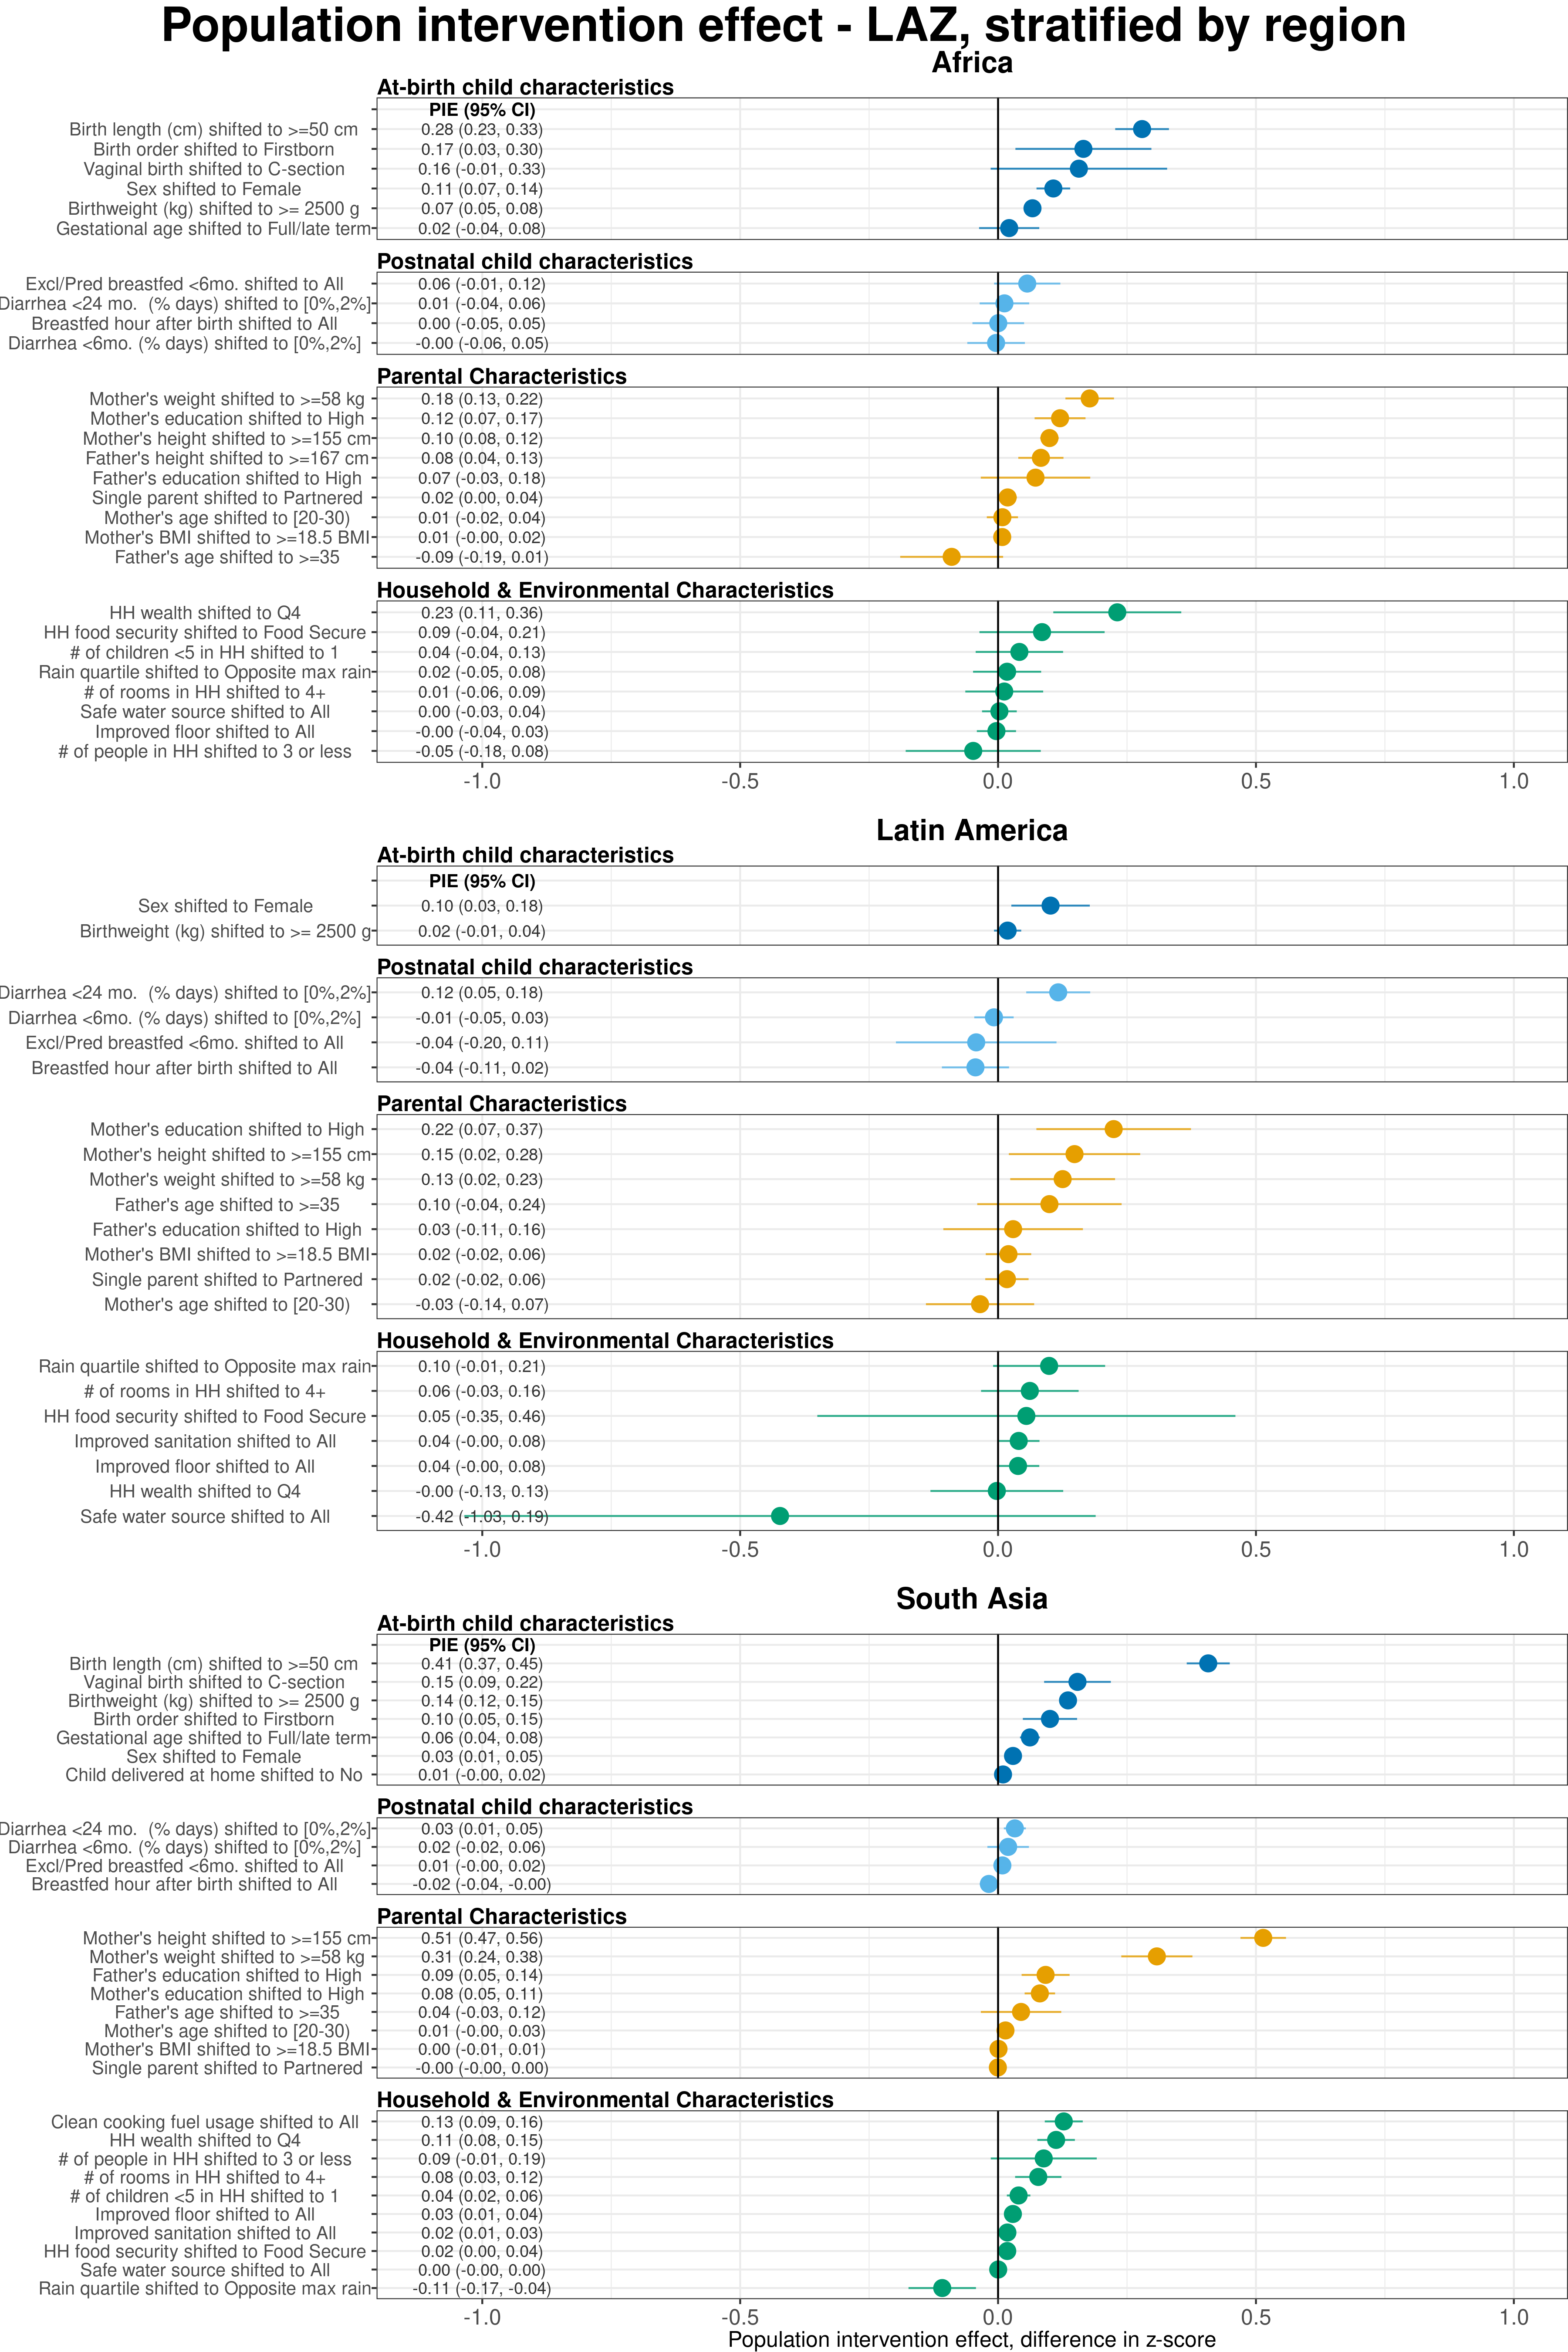
\includegraphics[width=62.5in]{C:/Users/andre/Documents/HBGDki/causes/ki-longitudinal-manuscripts/figures/manuscript-figure-composites/risk-factor/extended-data/fig-laz-PAR-strat-region_FE}
\textbf{Extended Data Figure 7 \textbar{} Region-stratified population attributable differences in length-for-age Z-scores estimated using fixed effects. }

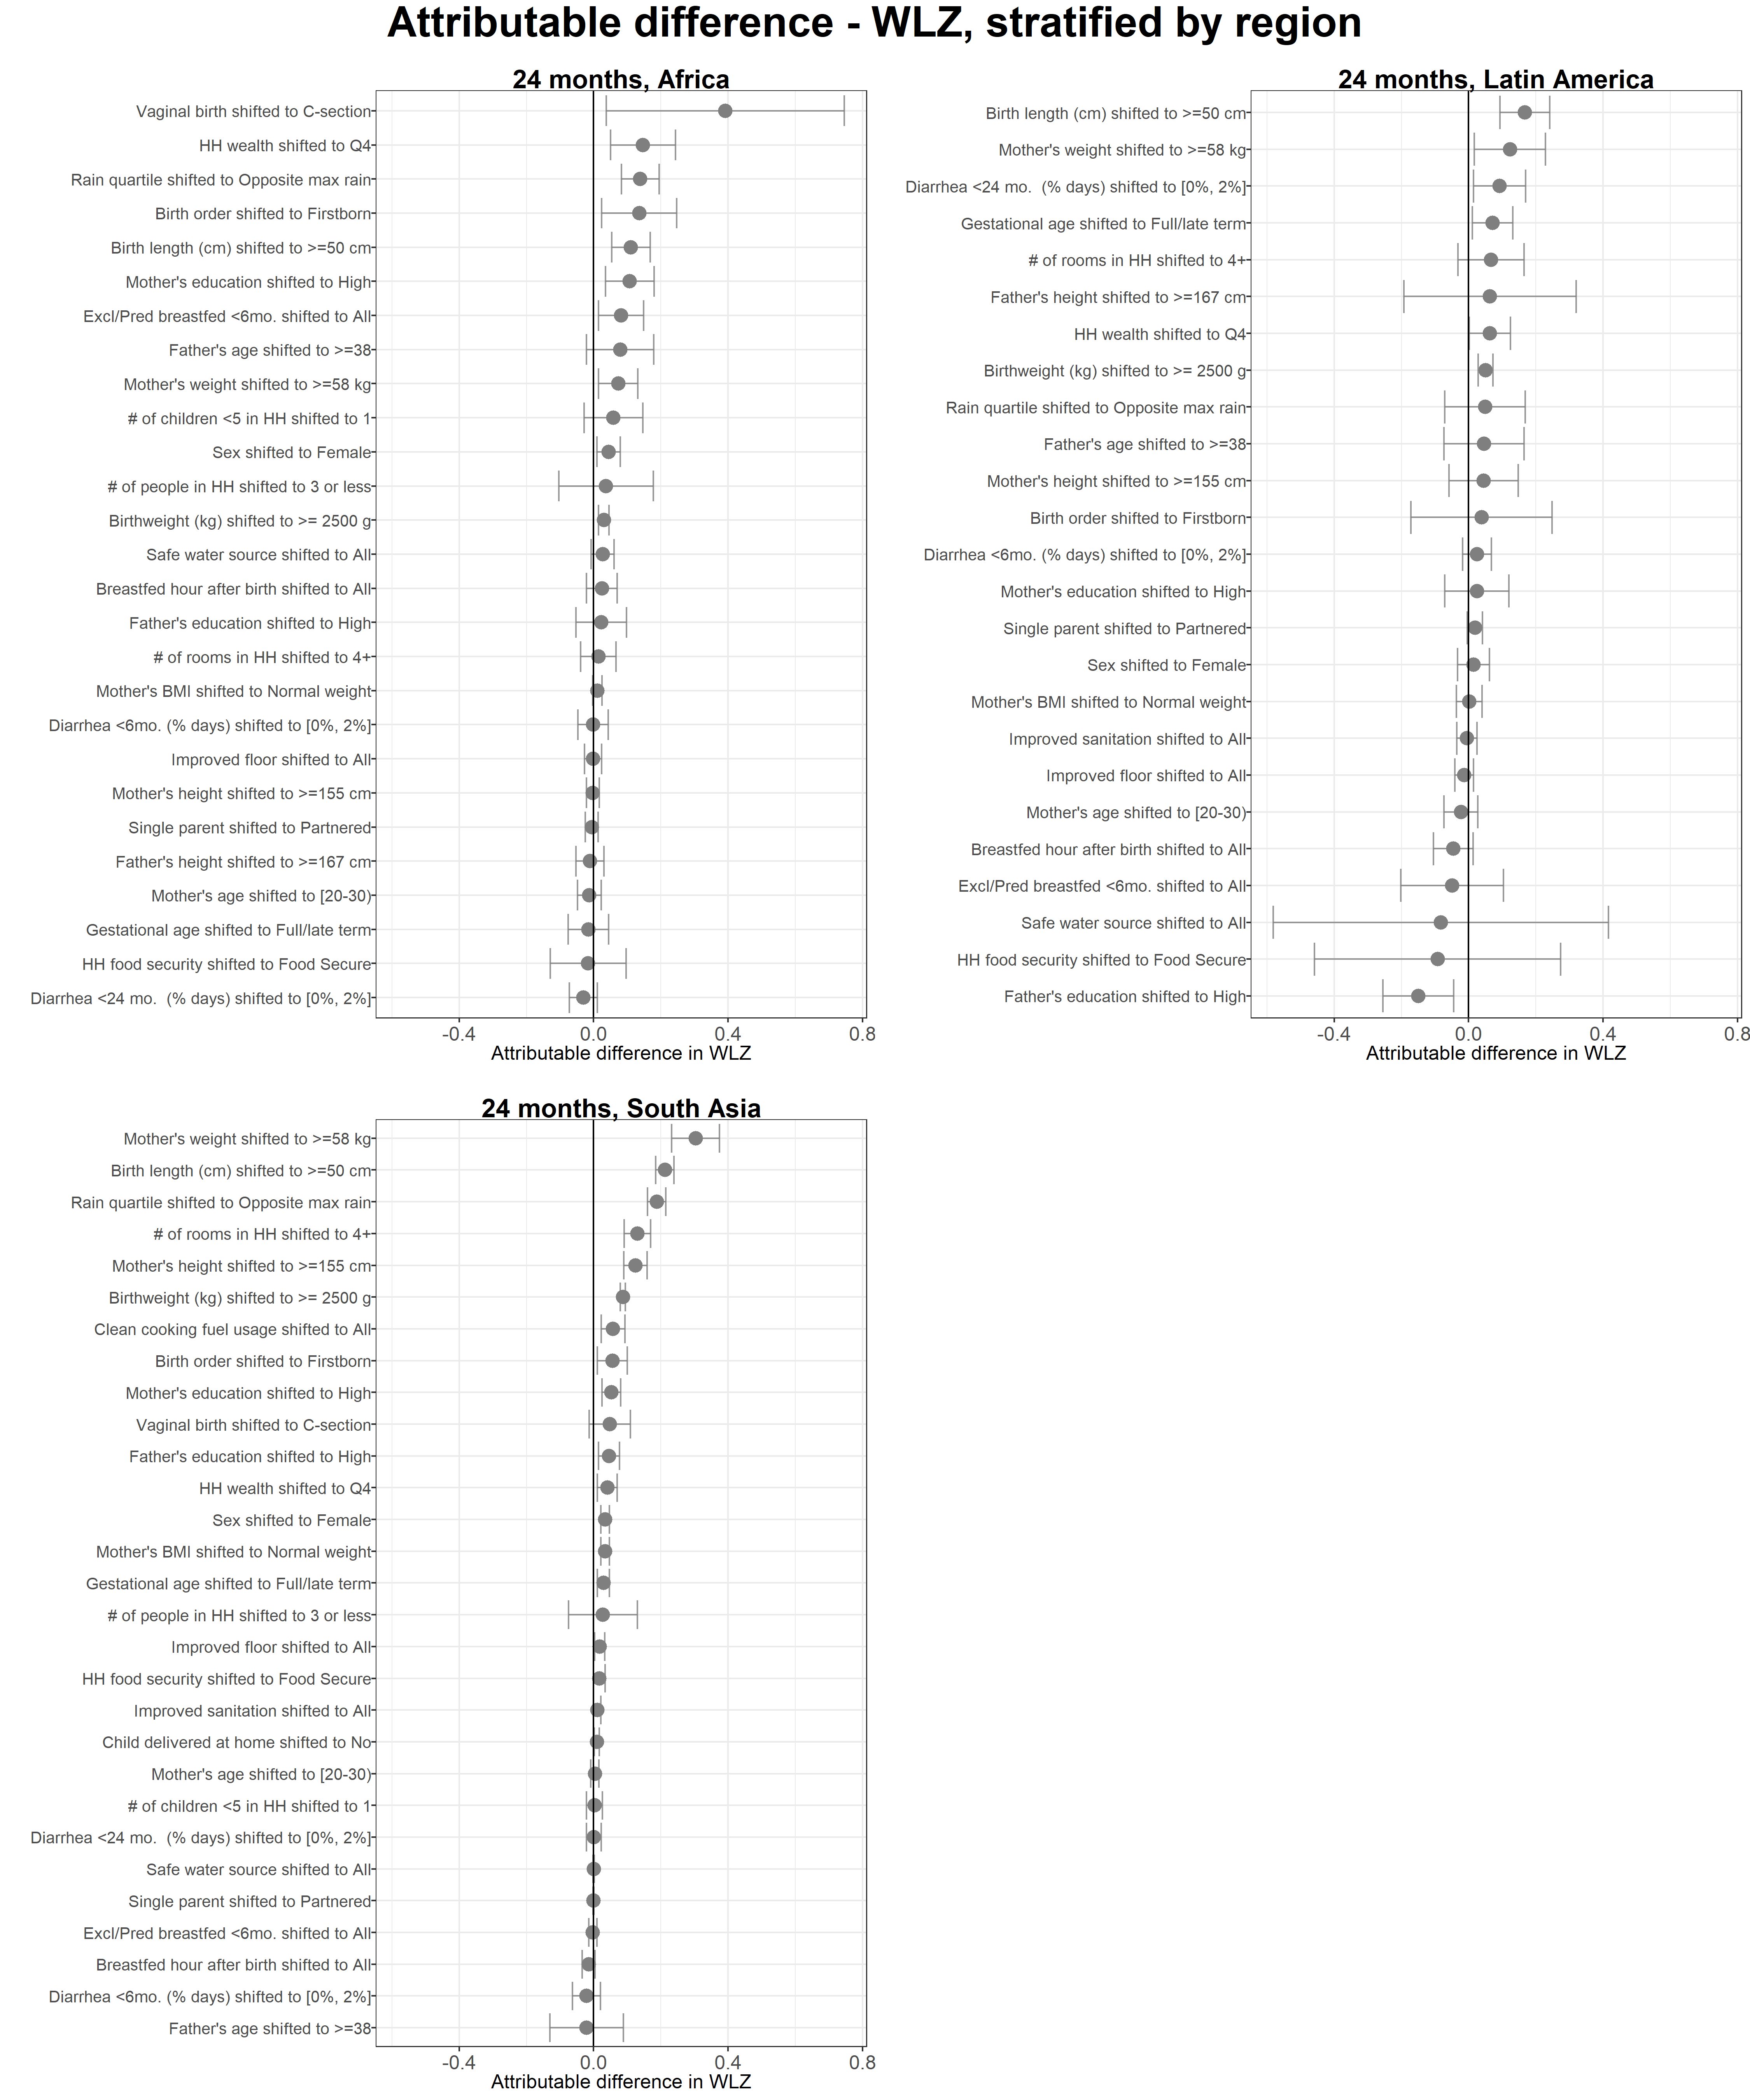
\includegraphics[width=62.5in]{C:/Users/andre/Documents/HBGDki/causes/ki-longitudinal-manuscripts/figures/manuscript-figure-composites/risk-factor/extended-data/fig-wlz-PAR-strat-region_FE}
\textbf{Extended Data Figure 8 \textbar{} Region-stratified population attributable differences in weight-for-length Z-scores estimated using fixed effects. }

\hypertarget{unadjusted}{%
\chapter{Unadjusted RF plots}\label{unadjusted}}

\raggedright

** {[}Coming soon{]} Will fill in with all primary plots, unadjusted **

\hypertarget{sens_splines}{%
\chapter{Sensitivity spline plots}\label{sens_splines}}

\raggedright

\hypertarget{primary-spline-figures---meta-analysis-of-cohort-specific-splines}{%
\subsection{Primary spline figures - meta-analysis of cohort specific splines}\label{primary-spline-figures---meta-analysis-of-cohort-specific-splines}}

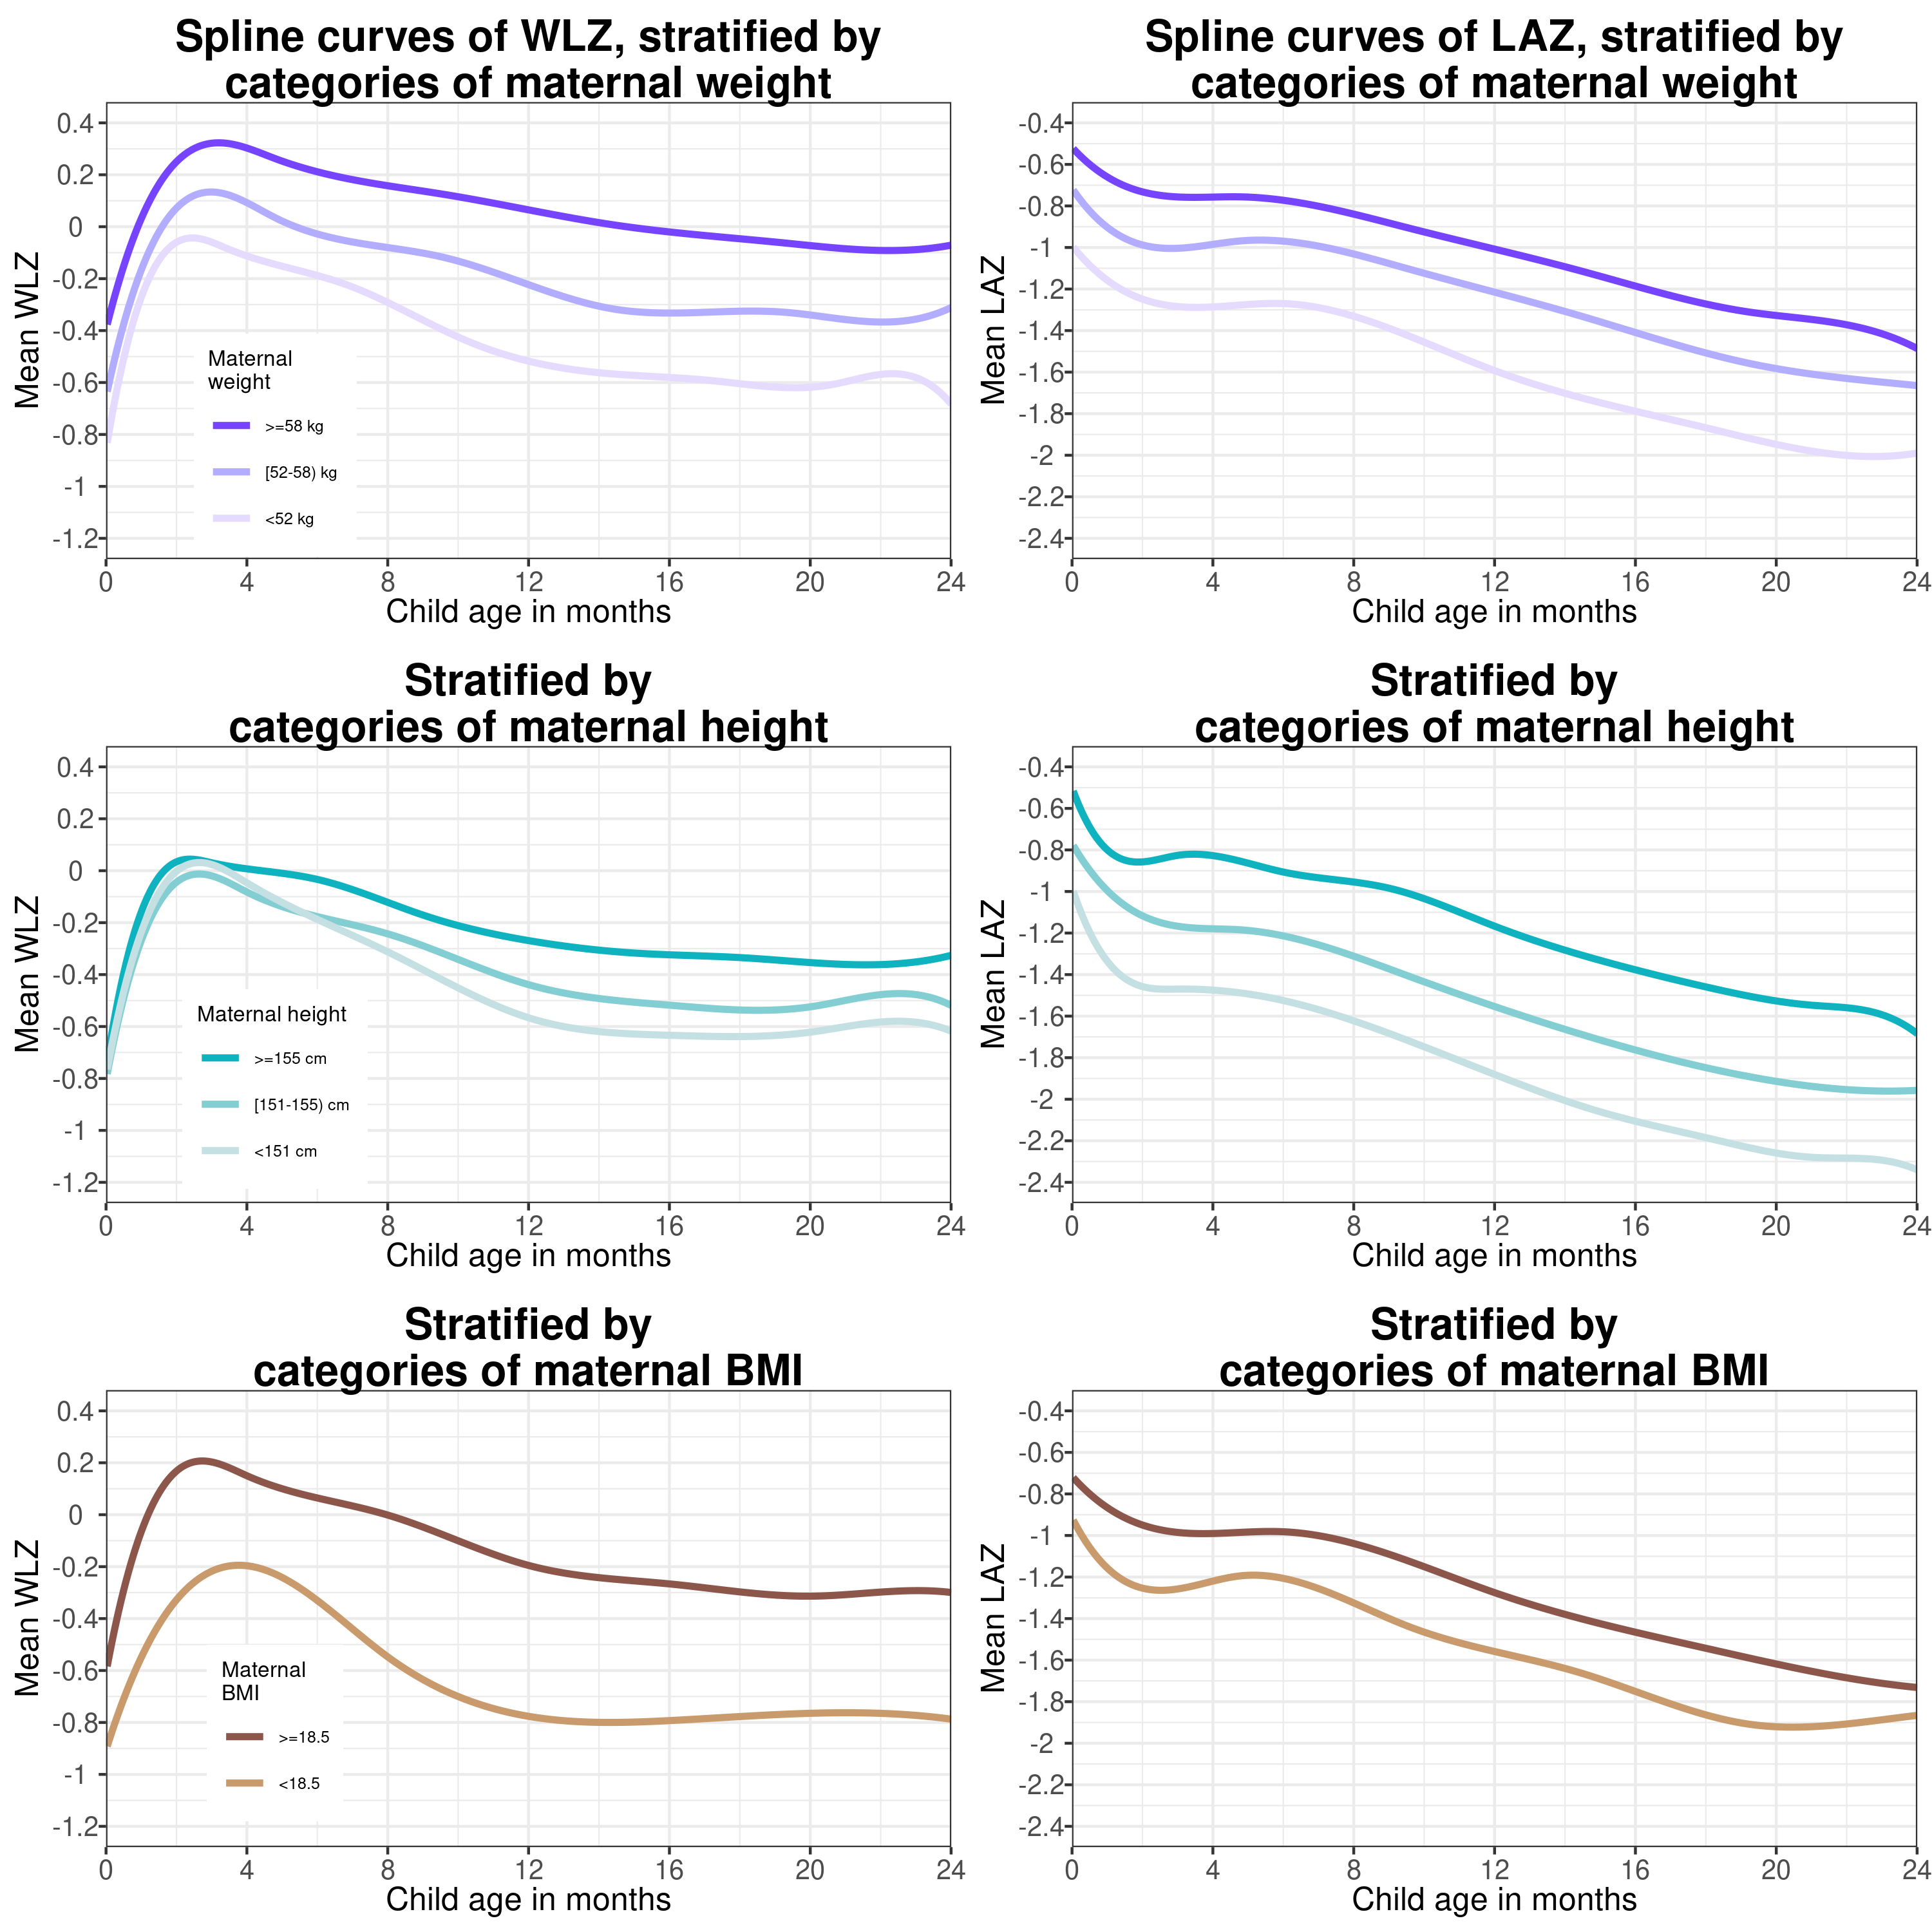
\includegraphics[width=41.67in]{C:/Users/andre/Documents/HBGDki/causes/ki-longitudinal-manuscripts/figures/risk-factor/spline_grid}

\hypertarget{spline-figures---meta-analysis-of-cohort-specific-splines-different-parameters}{%
\subsection{Spline figures - meta-analysis of cohort specific splines, different parameters}\label{spline-figures---meta-analysis-of-cohort-specific-splines-different-parameters}}

Centered at age = 1 says and with 6 degrees of freedom

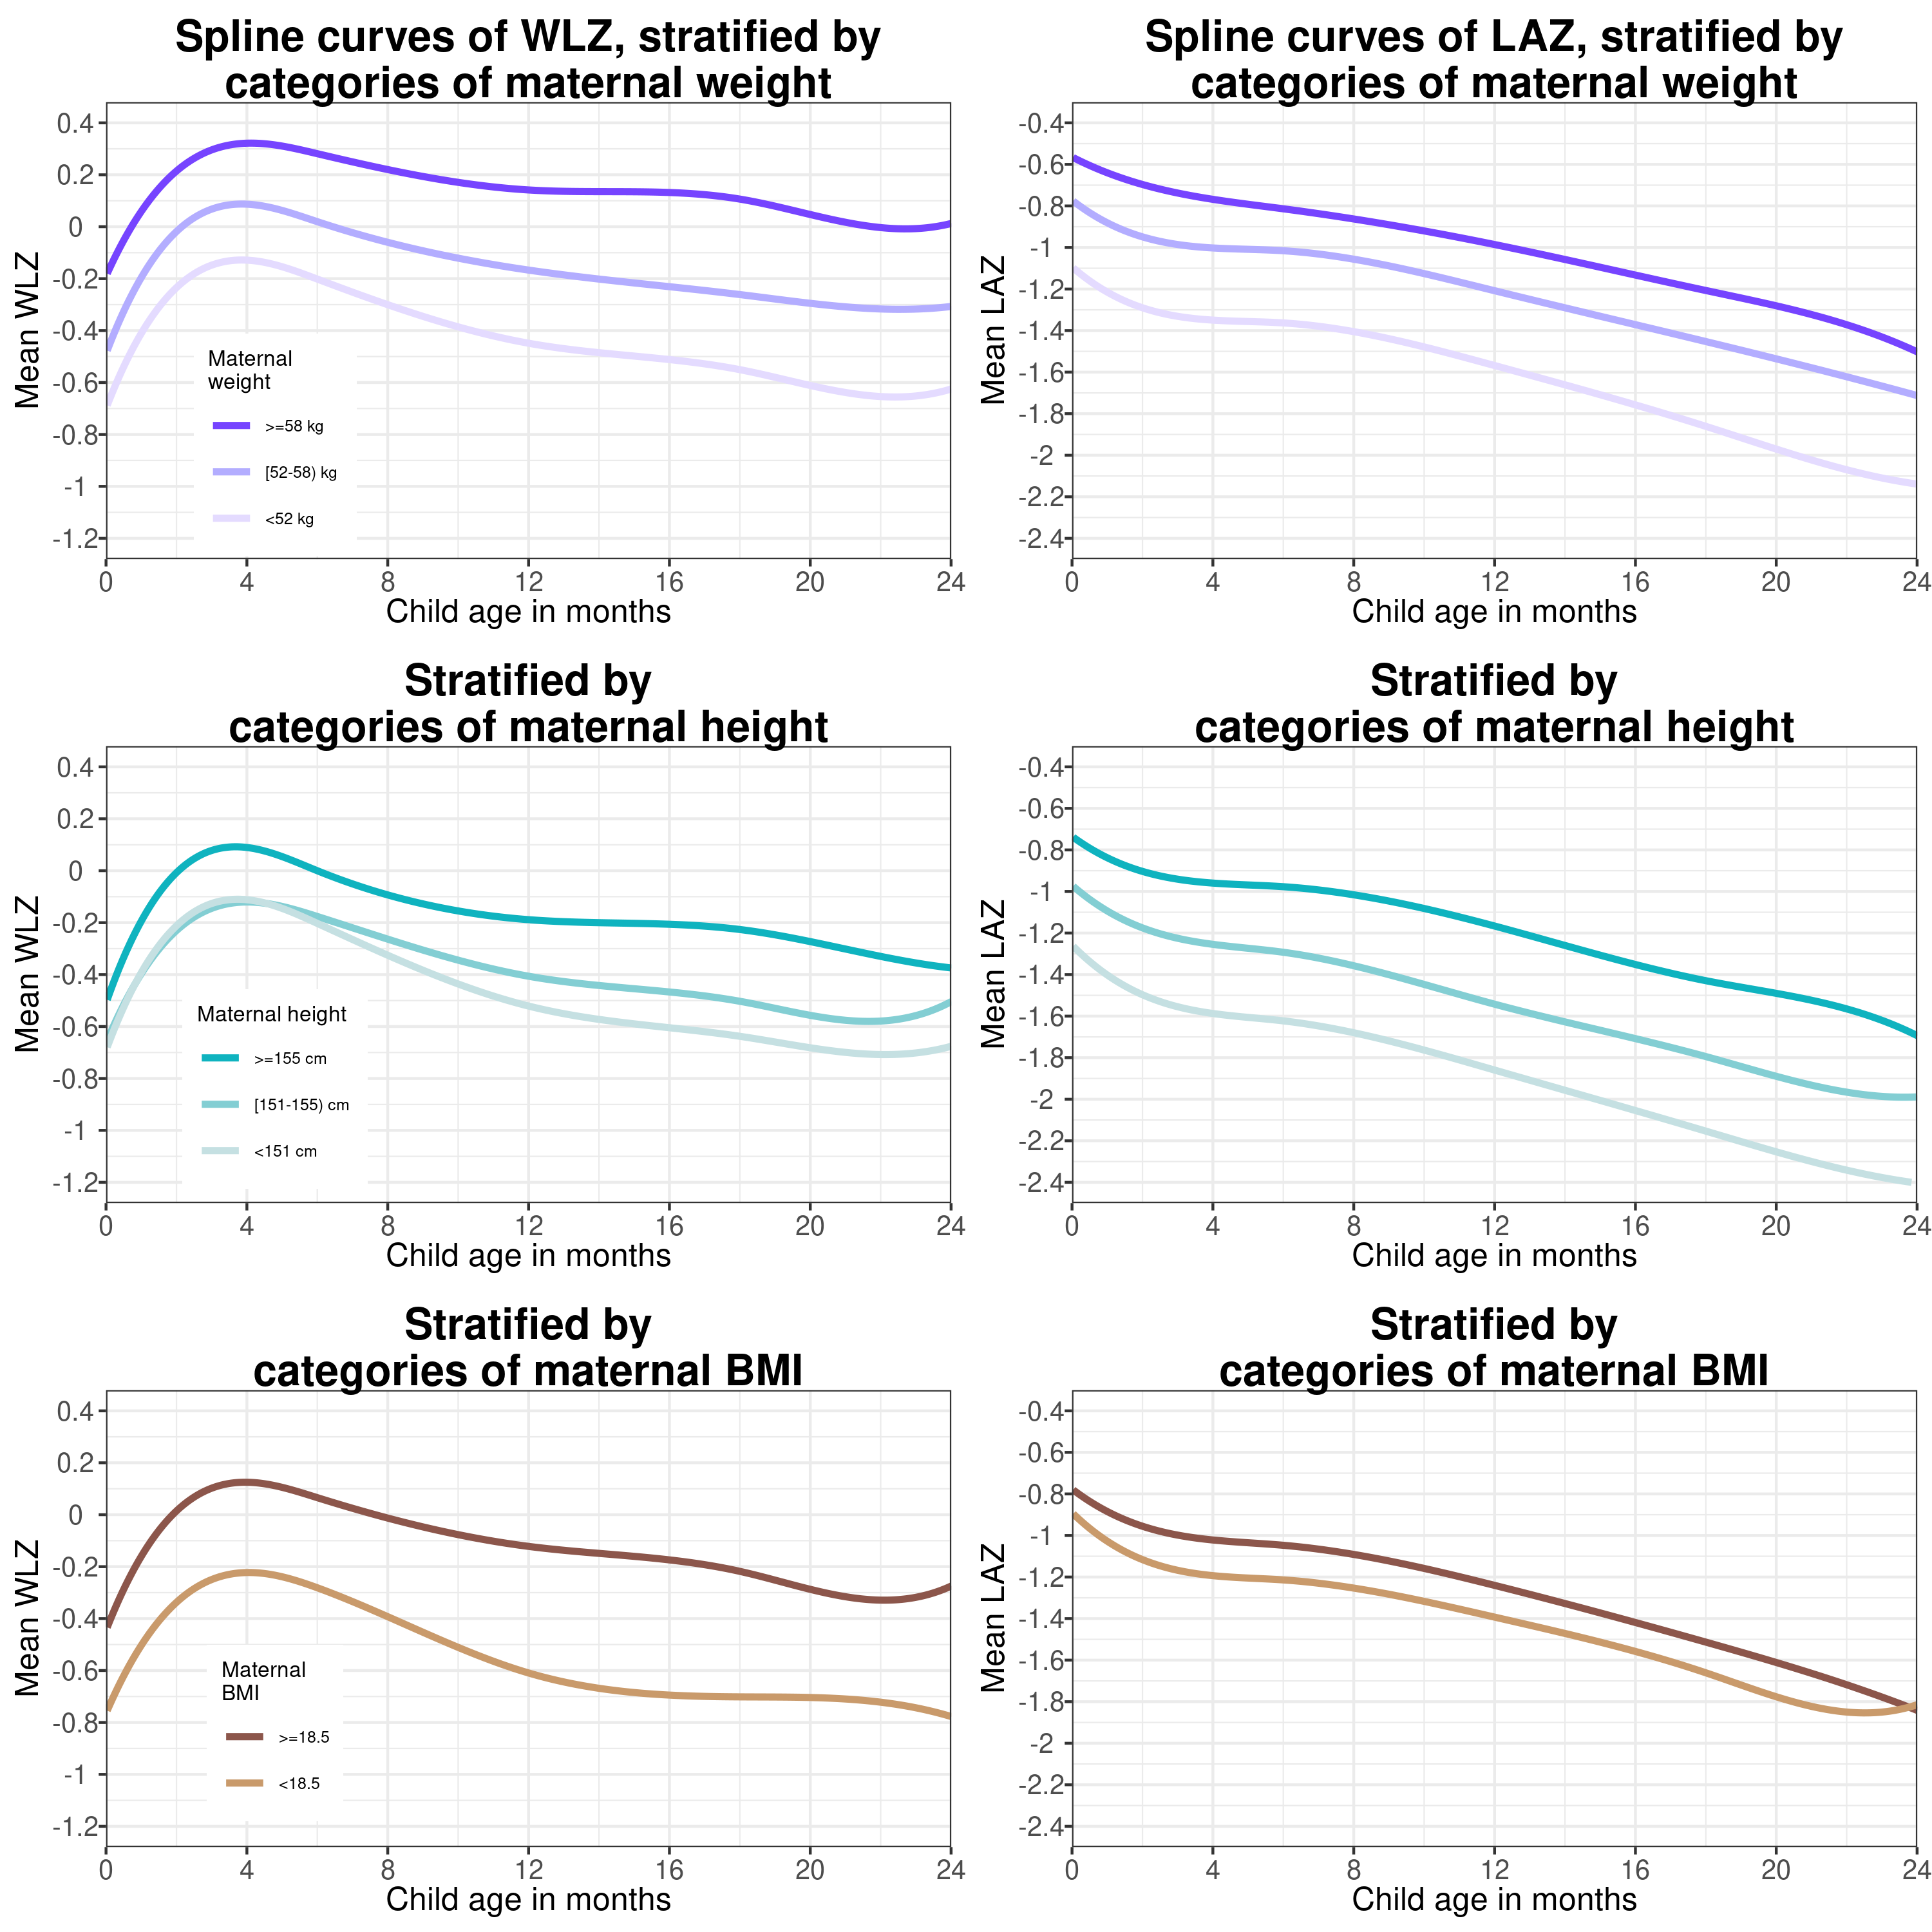
\includegraphics[width=41.67in]{C:/Users/andre/Documents/HBGDki/causes/ki-longitudinal-manuscripts/figures/risk-factor/spline_grid_sens}

\hypertarget{primary-spline-figures---single-spline-fit-to-all-the-data}{%
\subsection{Primary spline figures - Single spline fit to all the data}\label{primary-spline-figures---single-spline-fit-to-all-the-data}}

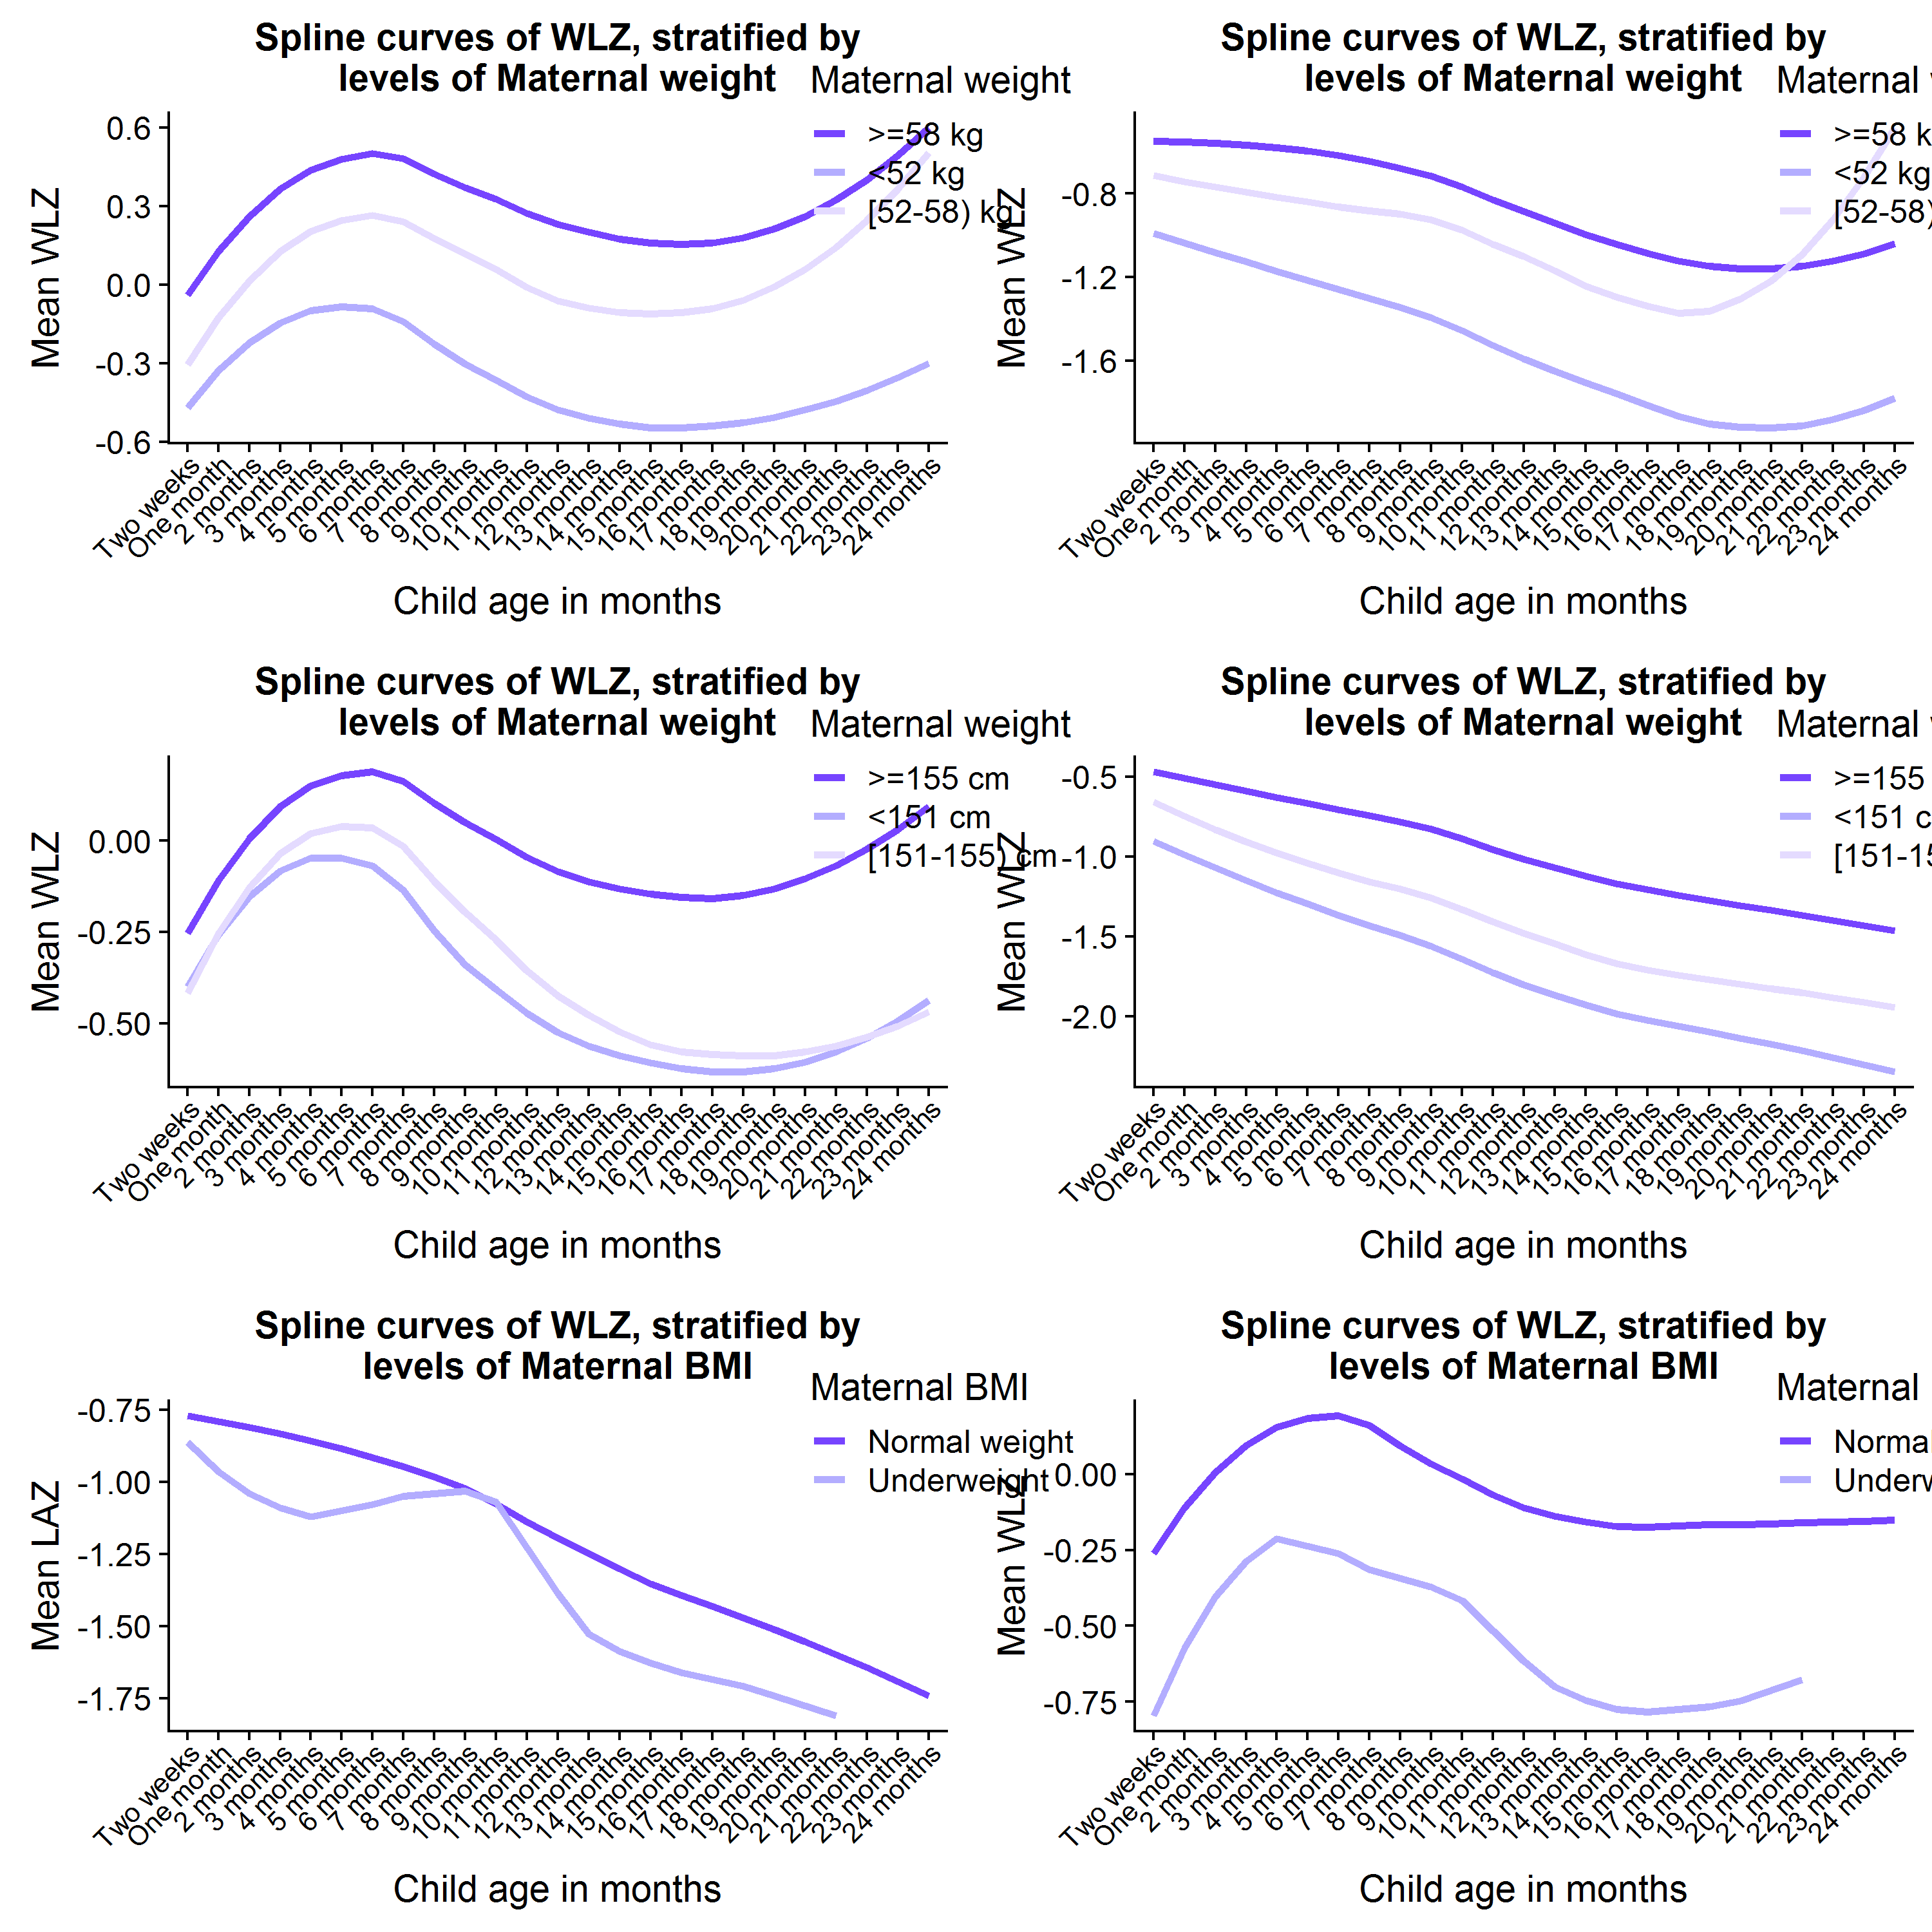
\includegraphics[width=41.67in]{C:/Users/andre/Documents/HBGDki/causes/ki-longitudinal-manuscripts/figures/risk-factor/spline_grid_sens2}

\hypertarget{primary-spline-figures---splines-fit-through-meta-analyses-of-monthly-means-of-z-scores}{%
\subsection{Primary spline figures - splines fit through meta-analyses of monthly means of Z-scores}\label{primary-spline-figures---splines-fit-through-meta-analyses-of-monthly-means-of-z-scores}}

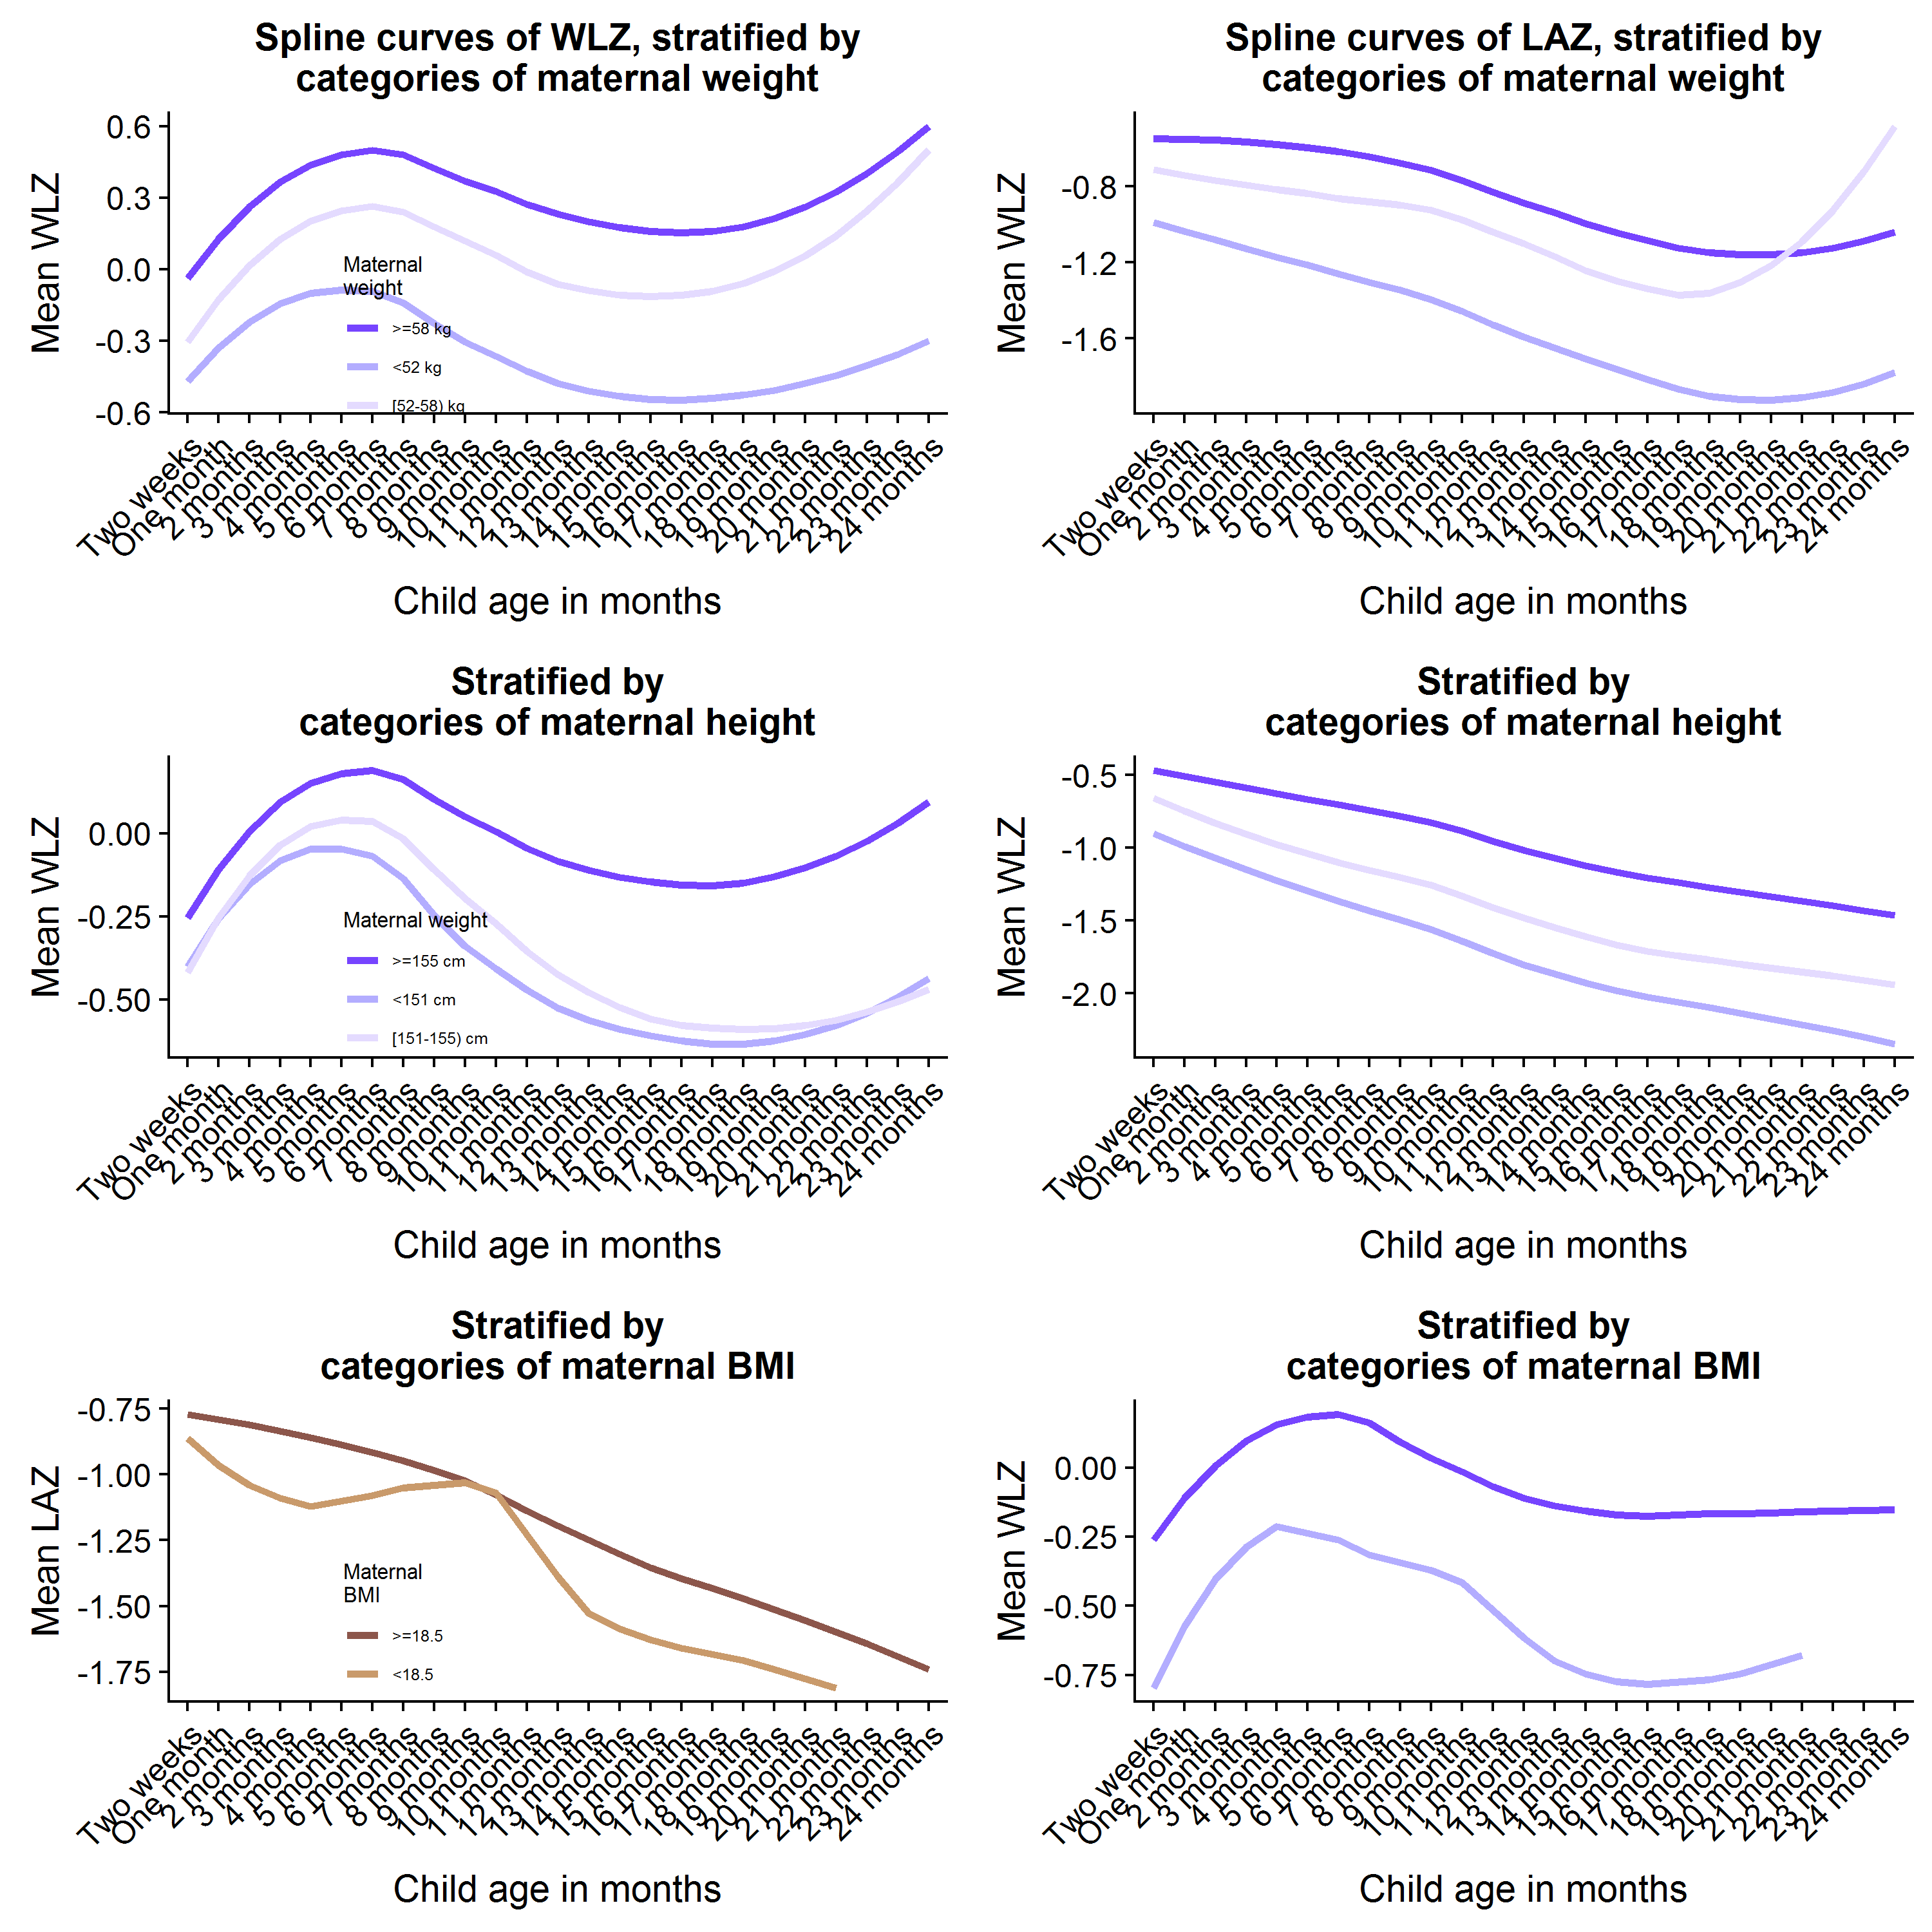
\includegraphics[width=41.67in]{C:/Users/andre/Documents/HBGDki/causes/ki-longitudinal-manuscripts/figures/risk-factor/spline_grid_sens3}

\hypertarget{rf_splines}{%
\chapter{spline-plots - all exposures}\label{rf_splines}}

\raggedright

\hypertarget{secondary-spline-figures---laz-stratified-by-levels-of-exposures}{%
\subsection{Secondary spline figures - LAZ stratified by levels of exposures}\label{secondary-spline-figures---laz-stratified-by-levels-of-exposures}}

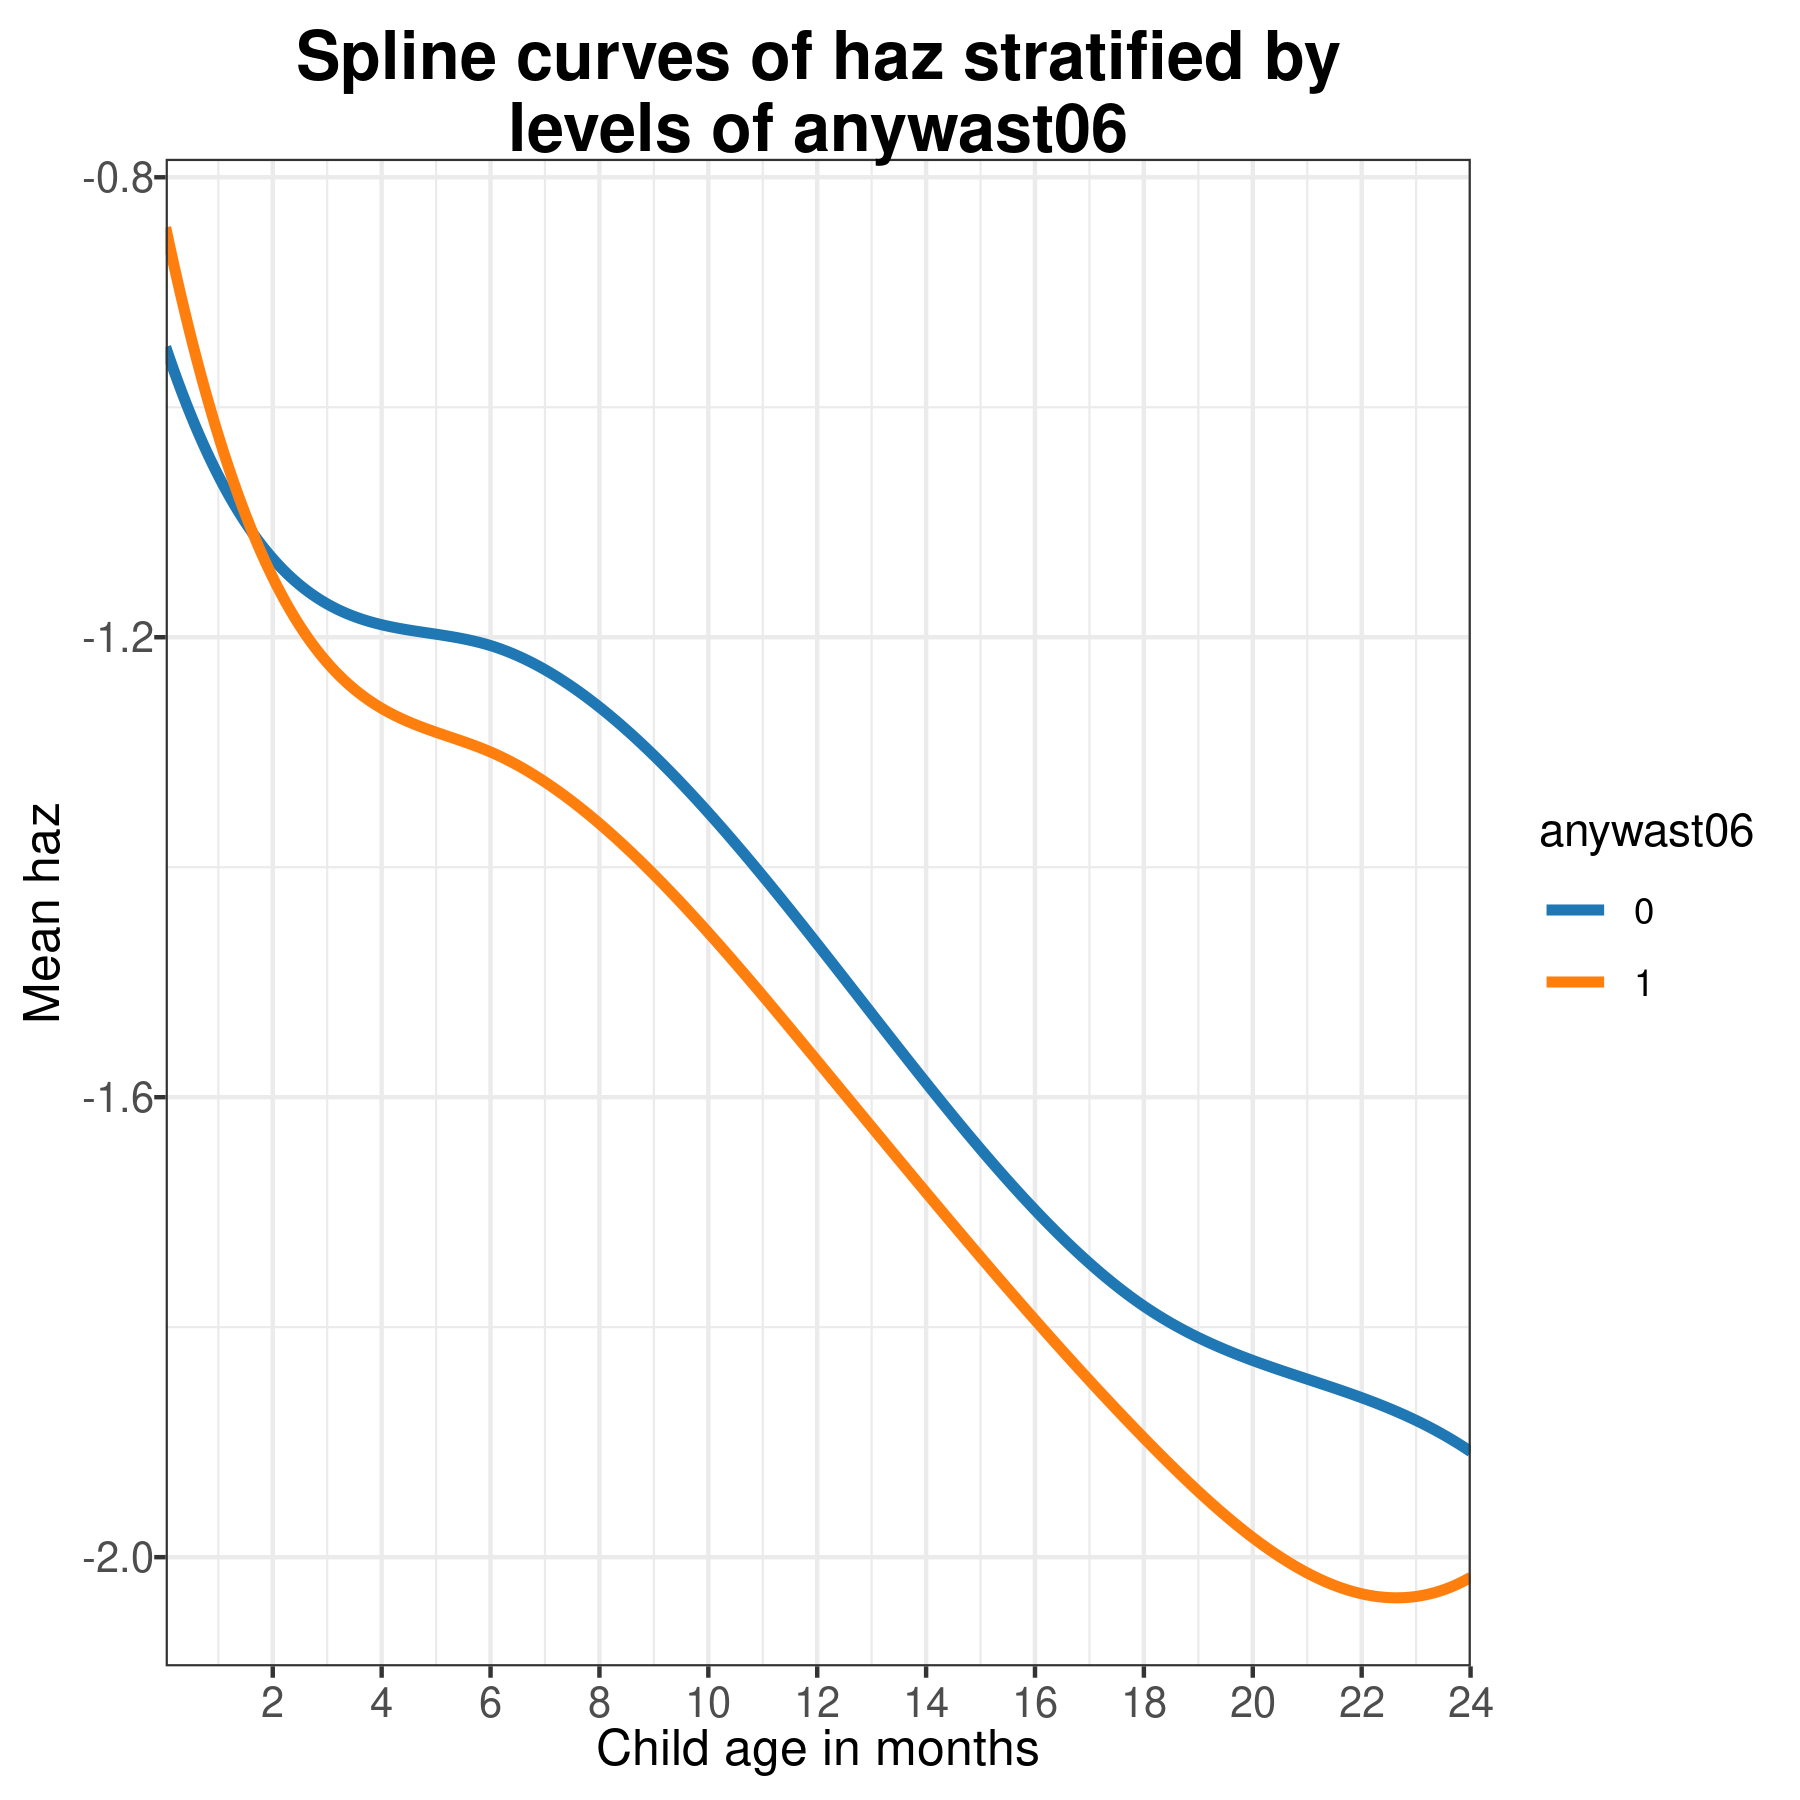
\includegraphics[width=25in]{C:/Users/andre/Documents/HBGDki/causes/ki-longitudinal-manuscripts/figures/risk-factor/spline-plots/haz-anywast06-spline}
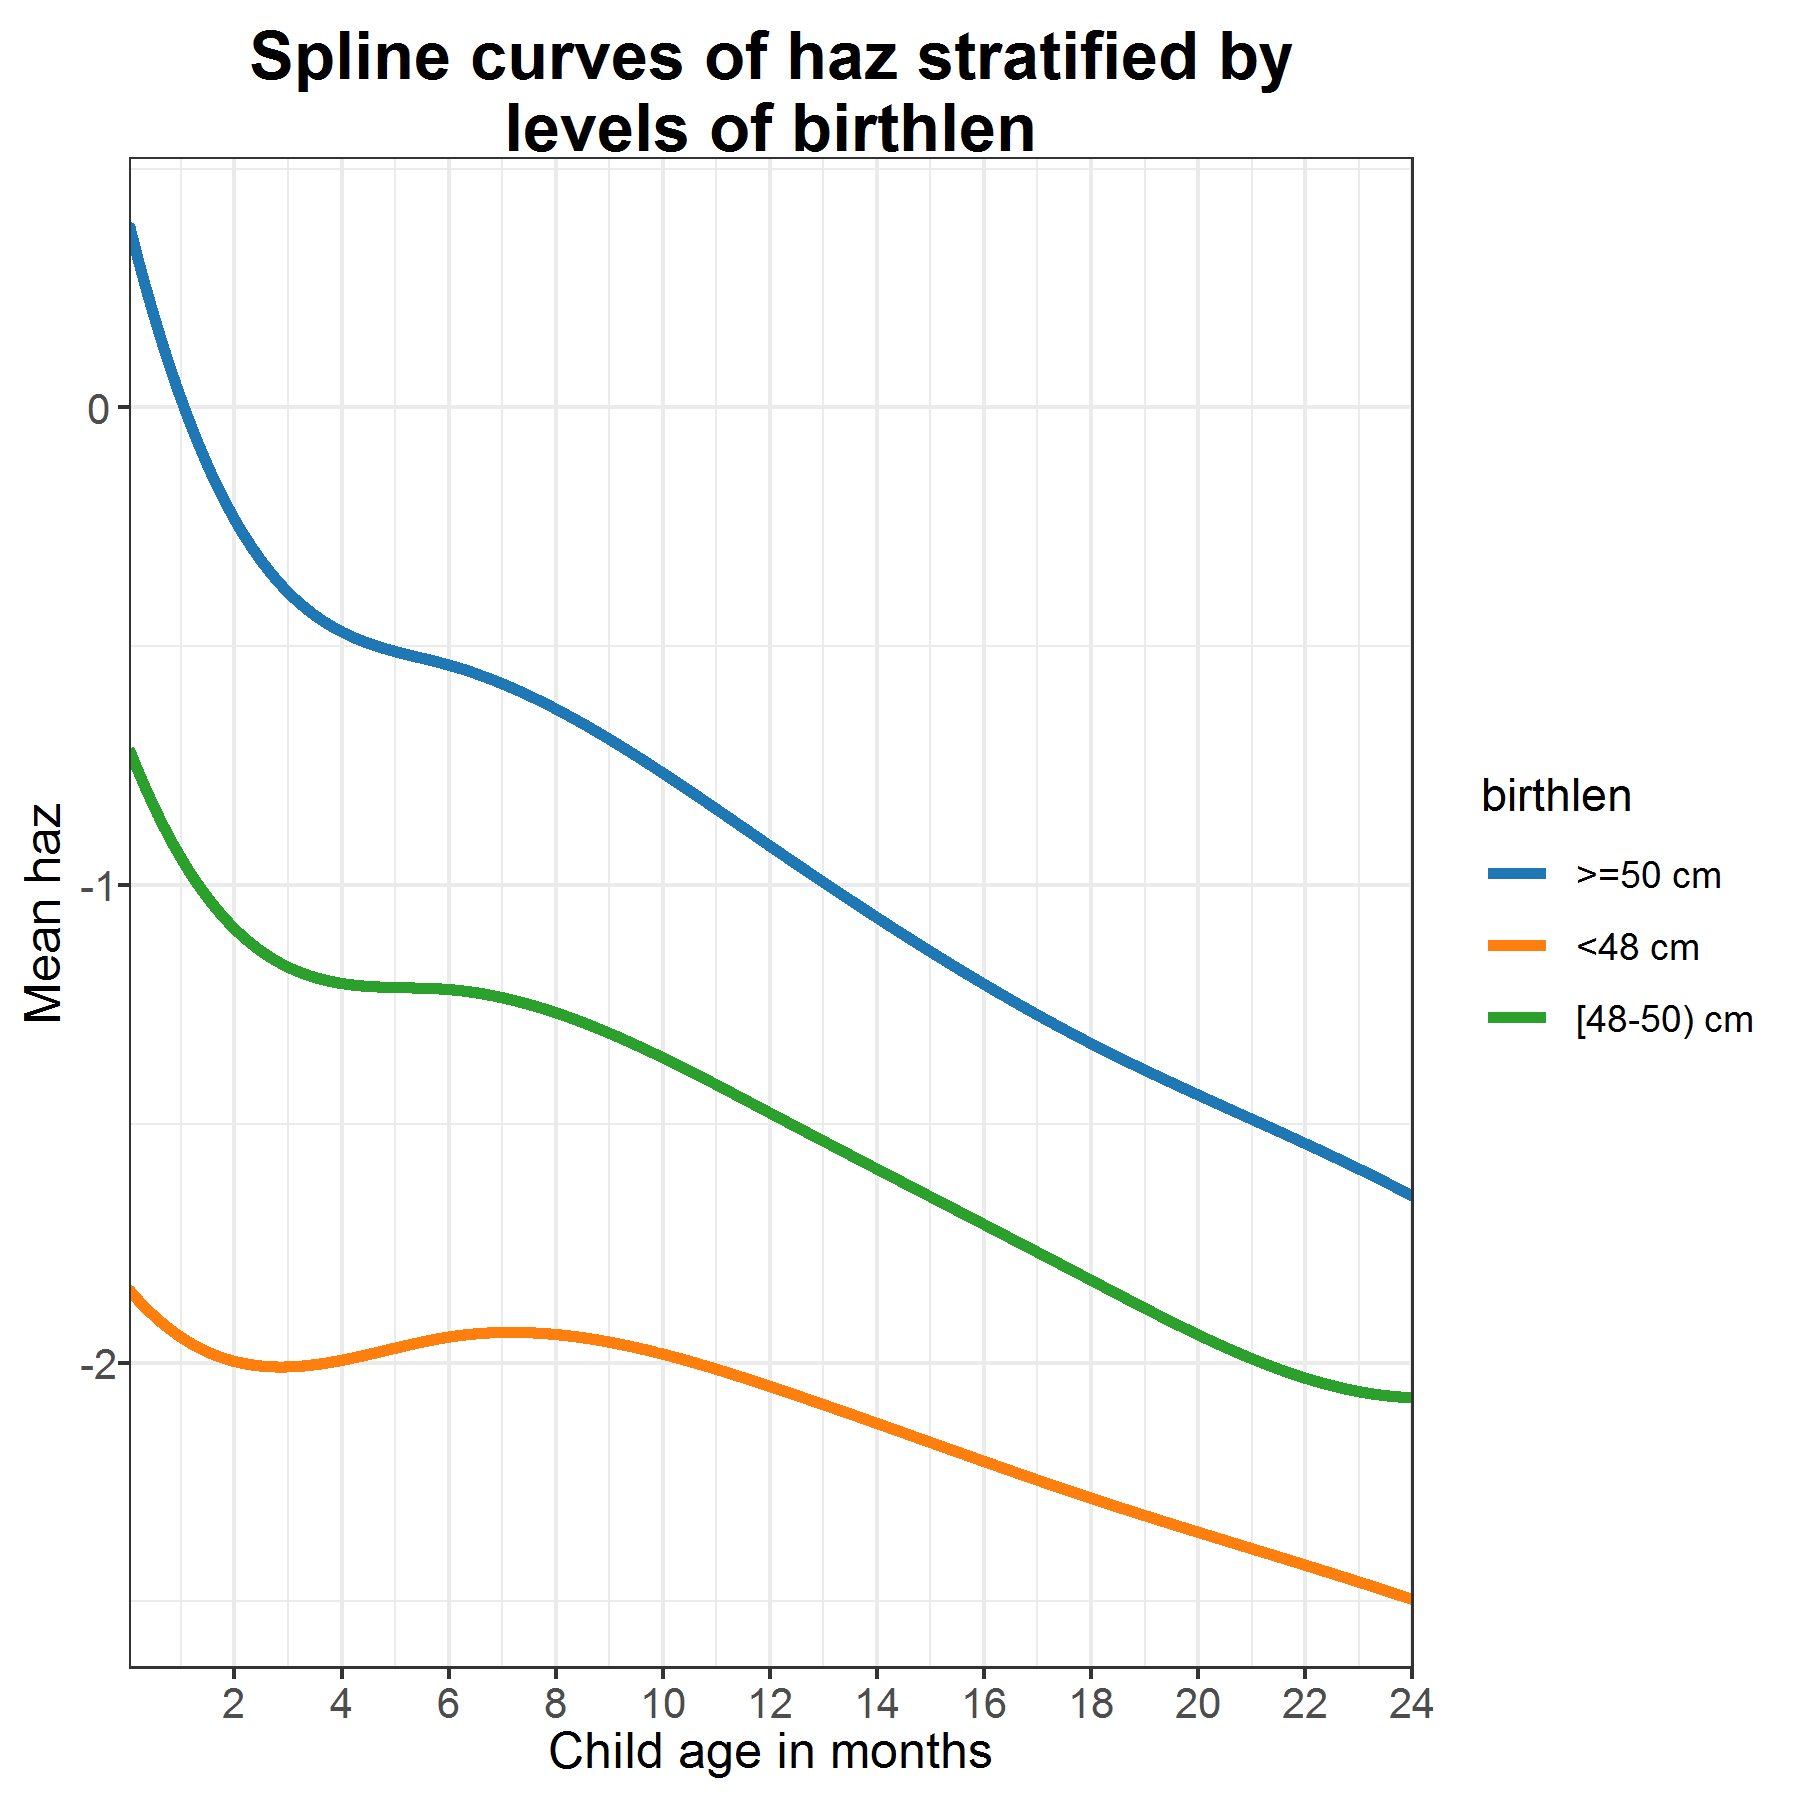
\includegraphics[width=25in]{C:/Users/andre/Documents/HBGDki/causes/ki-longitudinal-manuscripts/figures/risk-factor/spline-plots/haz-birthlen-spline}
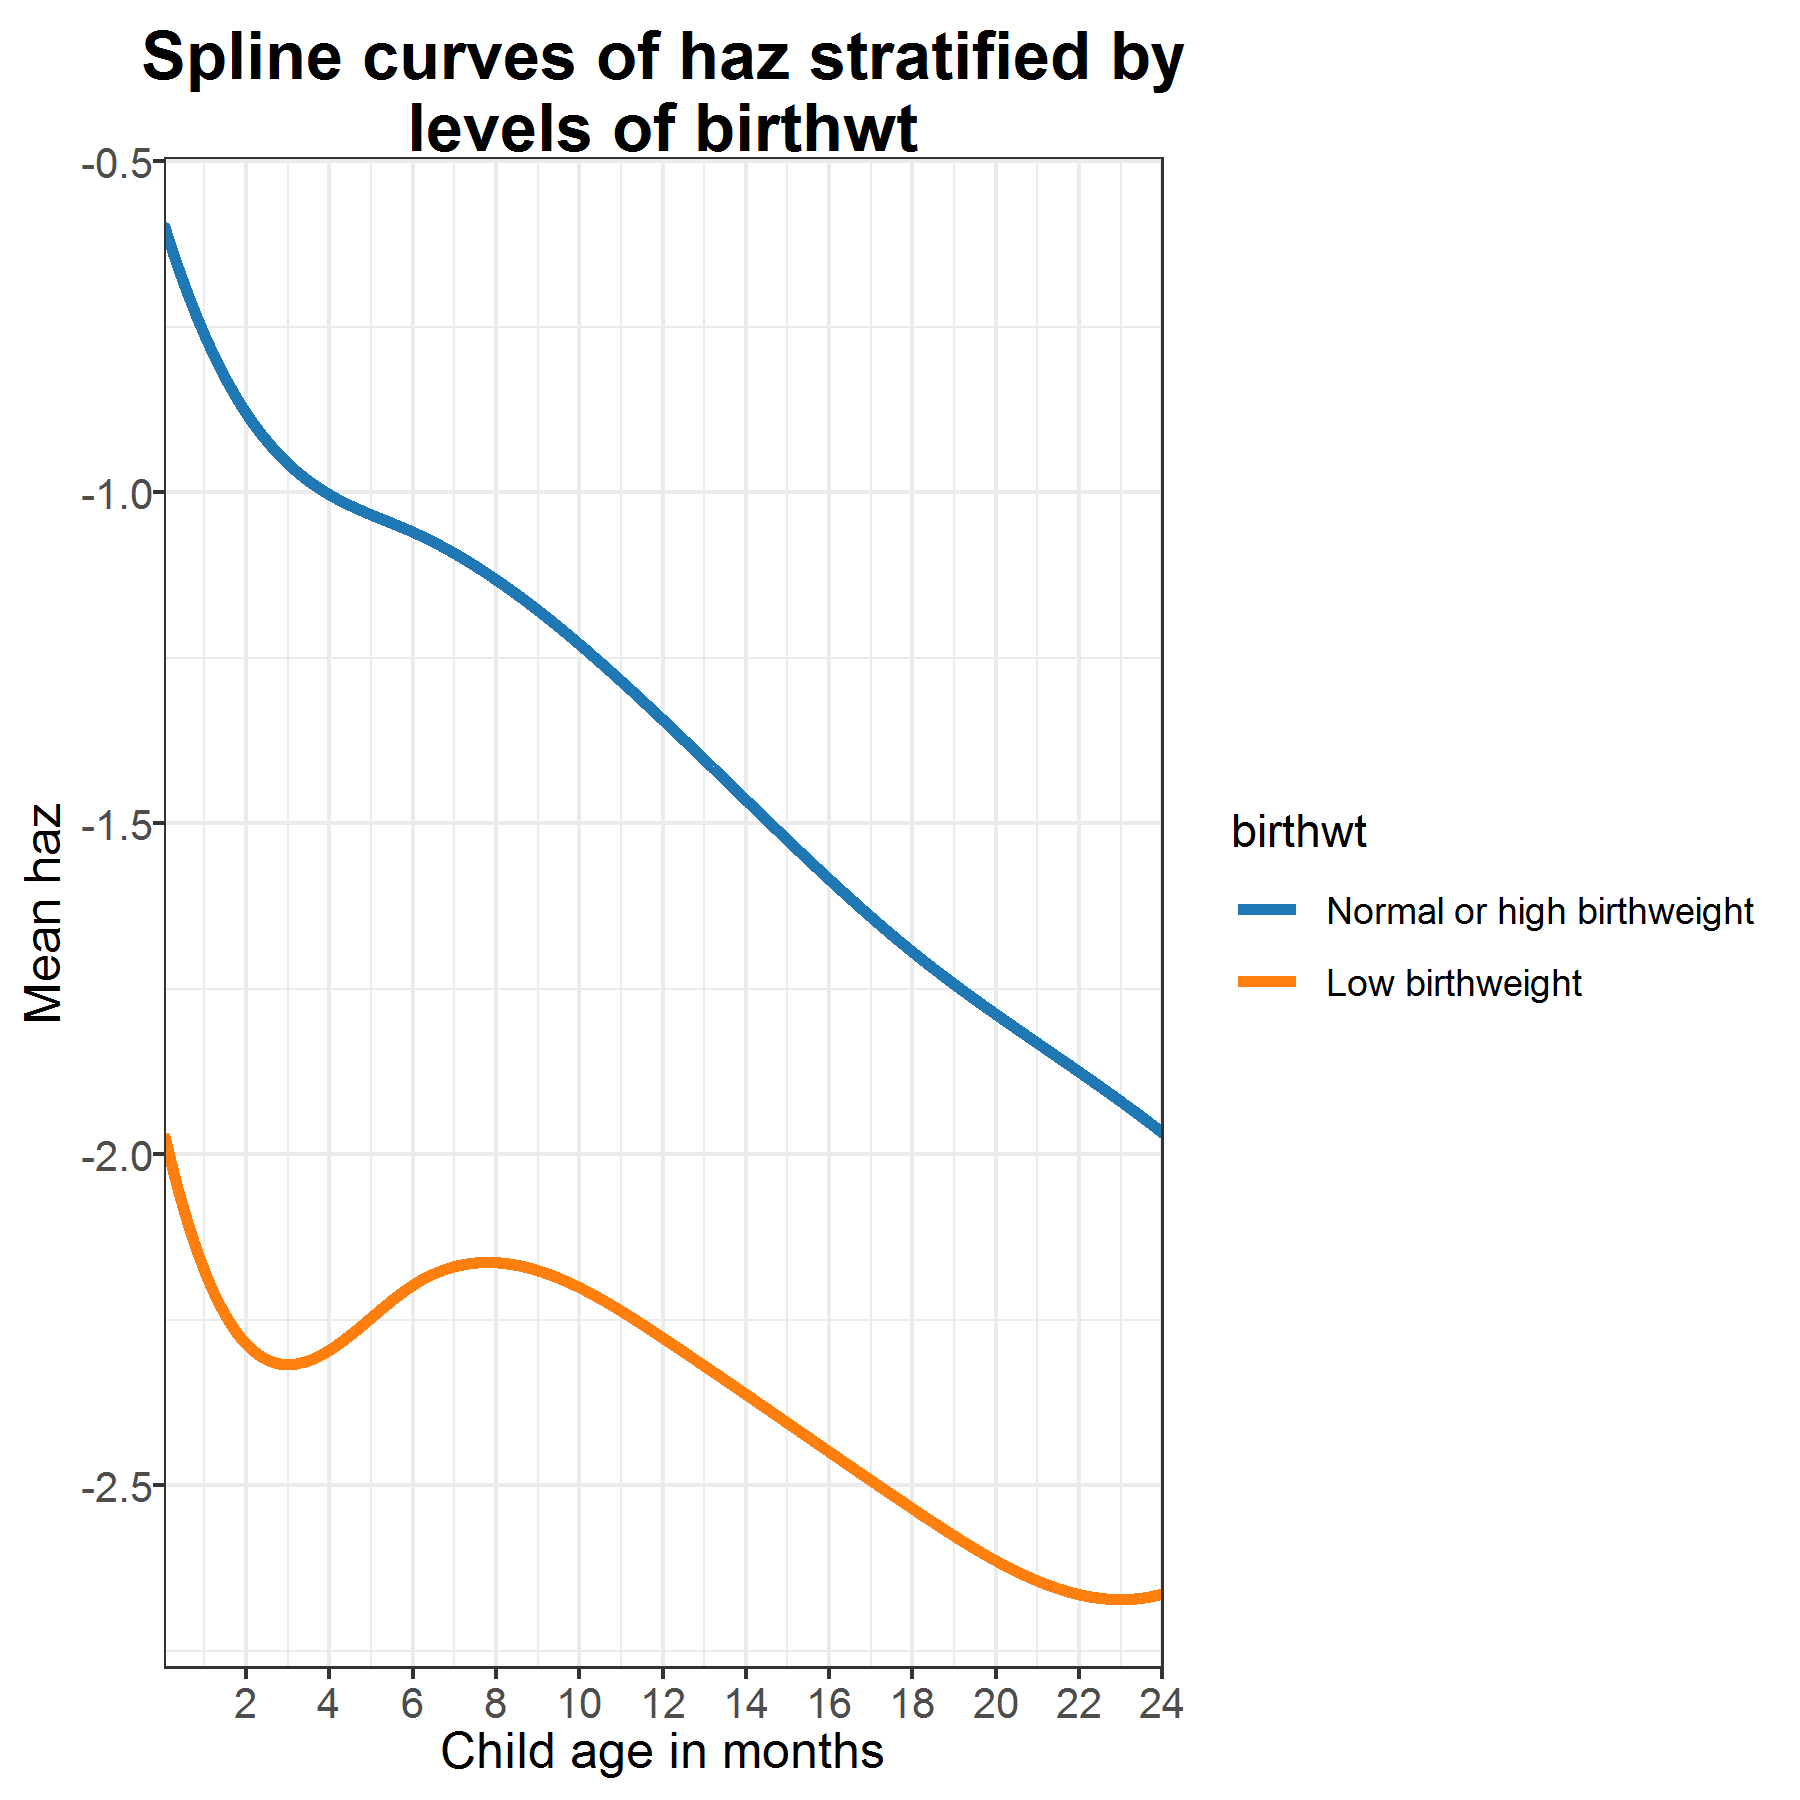
\includegraphics[width=25in]{C:/Users/andre/Documents/HBGDki/causes/ki-longitudinal-manuscripts/figures/risk-factor/spline-plots/haz-birthwt-spline}
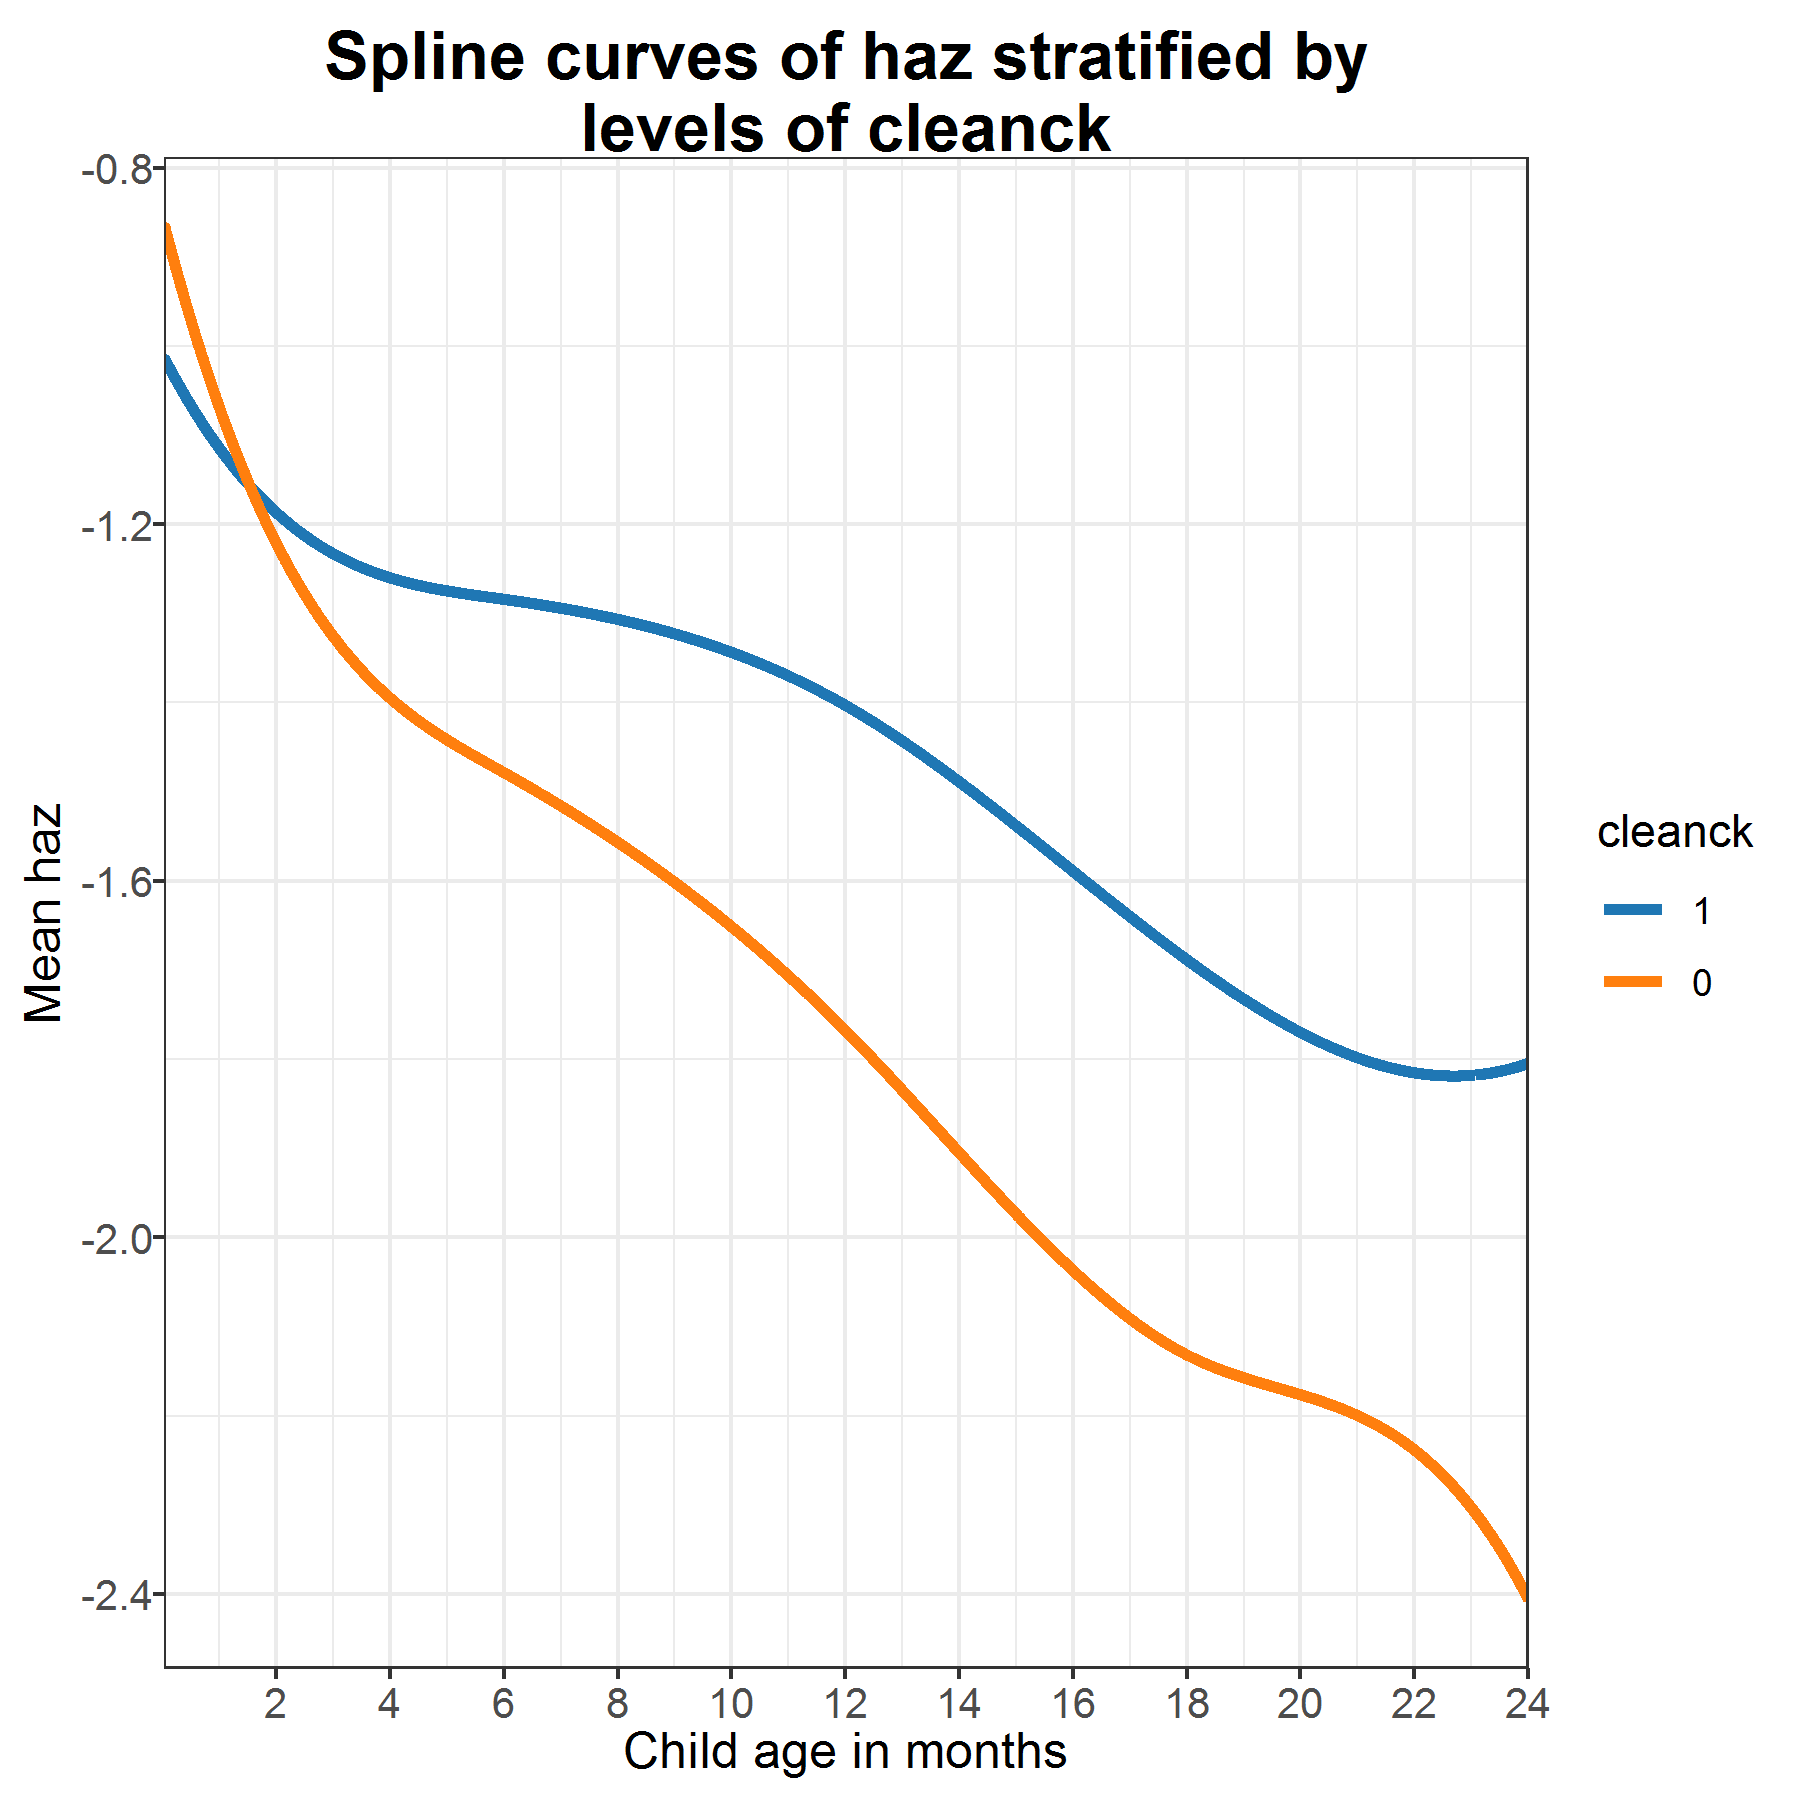
\includegraphics[width=25in]{C:/Users/andre/Documents/HBGDki/causes/ki-longitudinal-manuscripts/figures/risk-factor/spline-plots/haz-cleanck-spline}
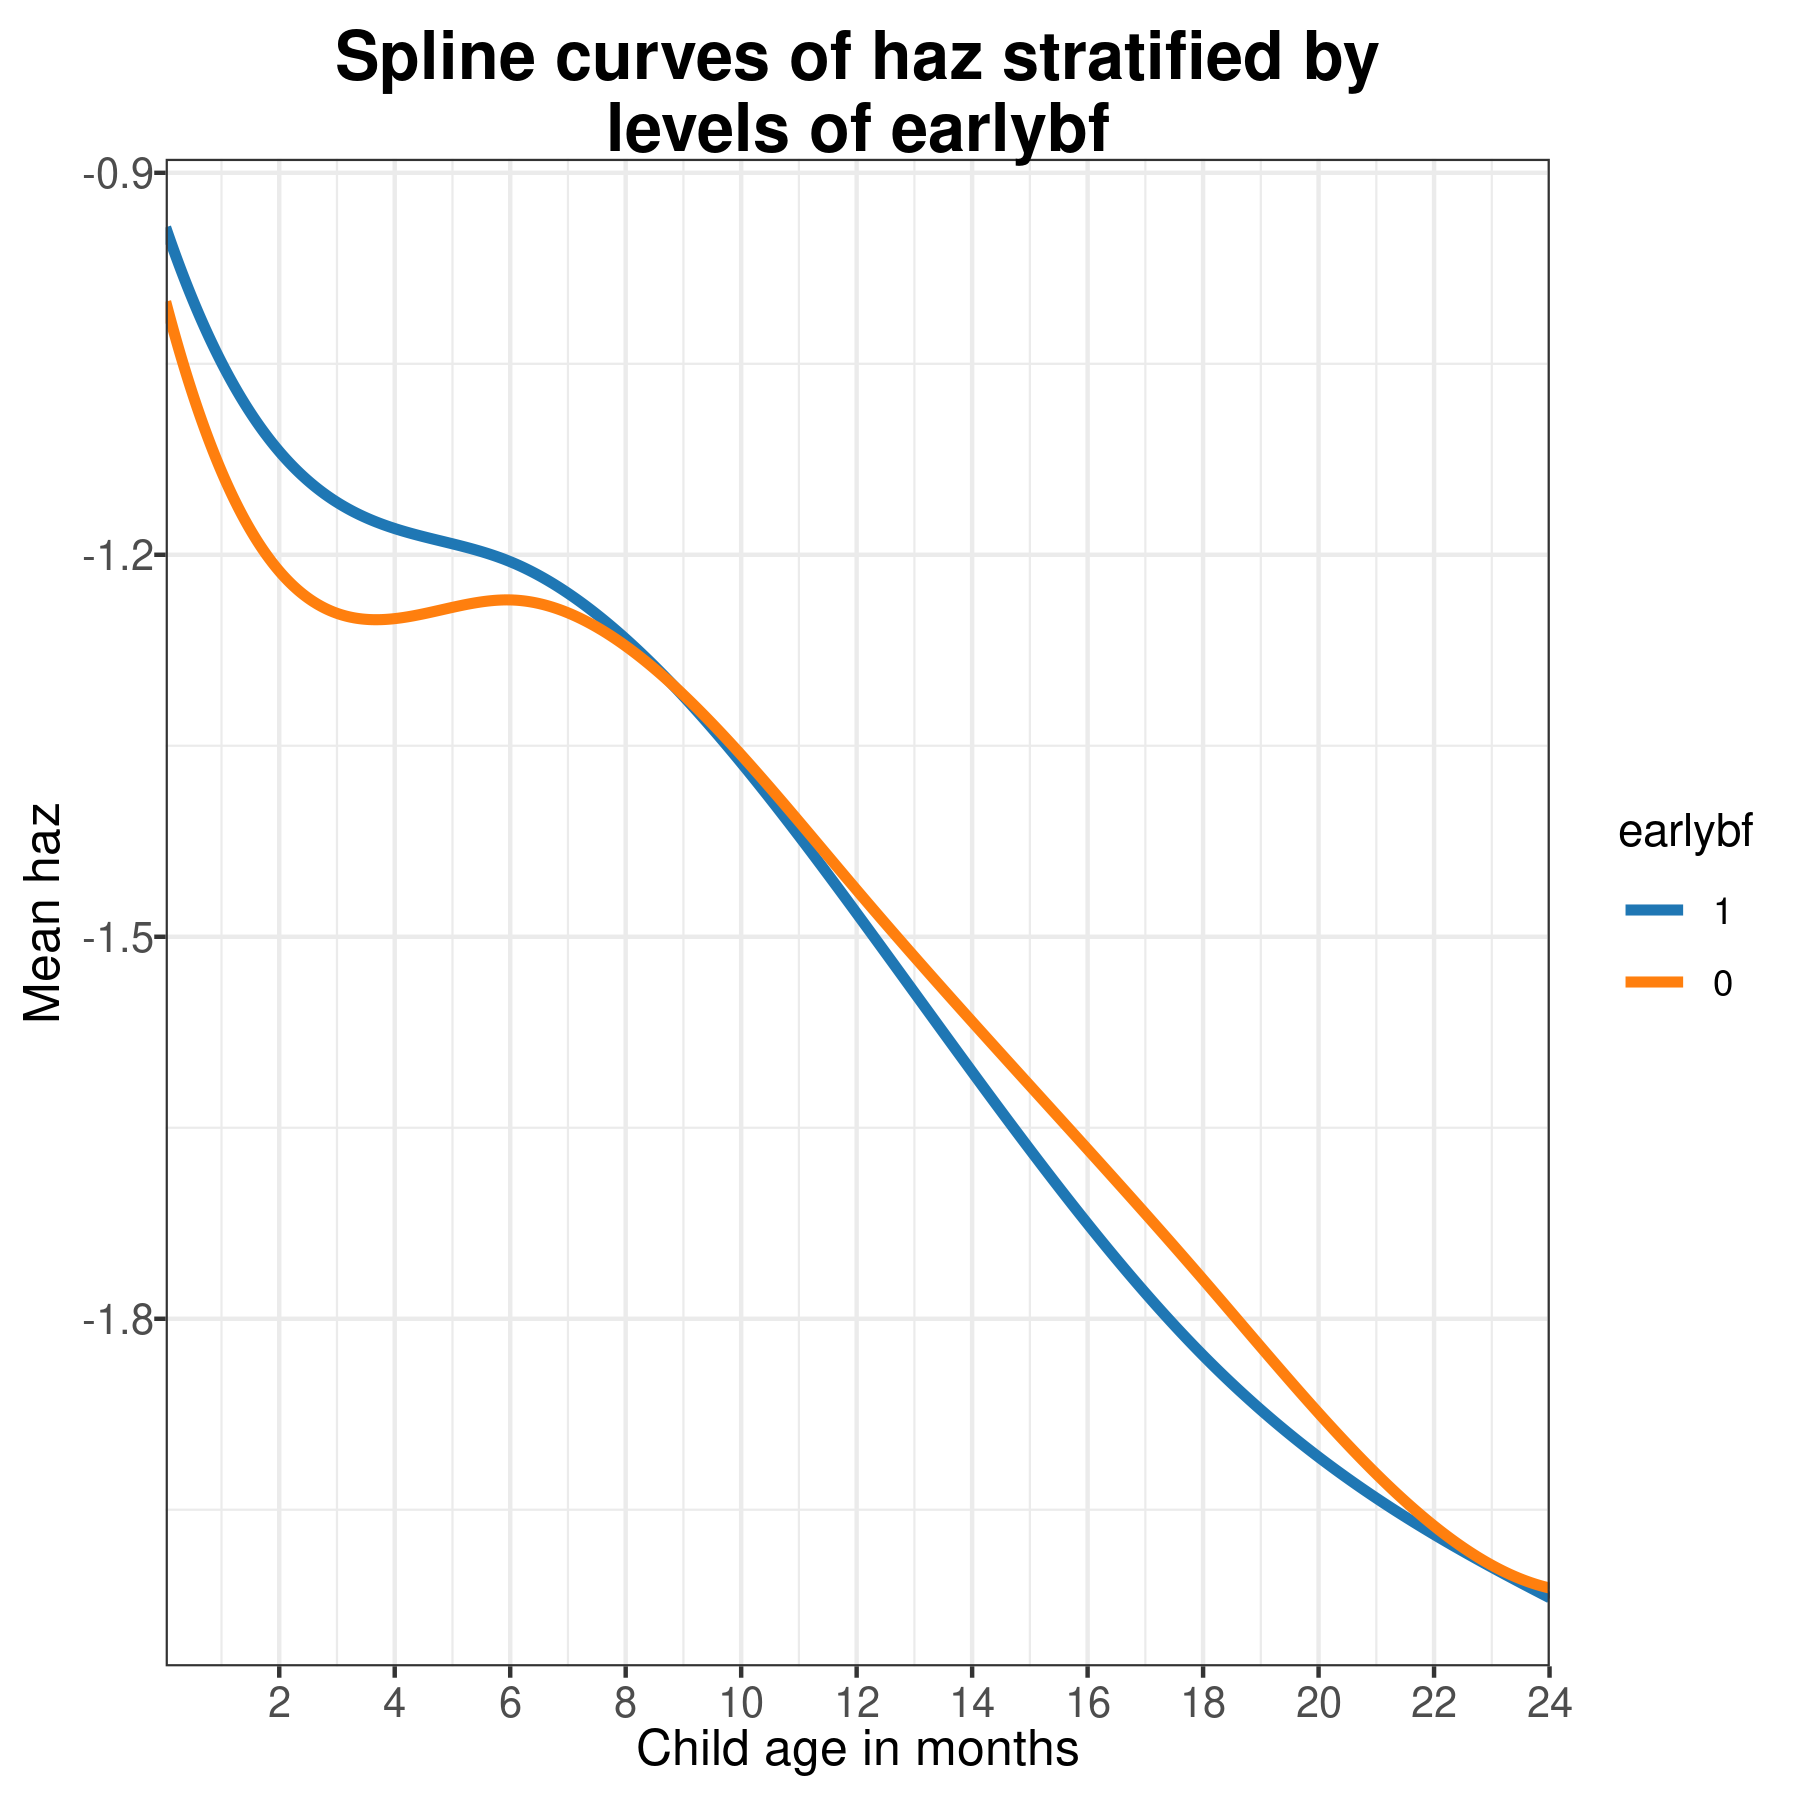
\includegraphics[width=25in]{C:/Users/andre/Documents/HBGDki/causes/ki-longitudinal-manuscripts/figures/risk-factor/spline-plots/haz-earlybf-spline}
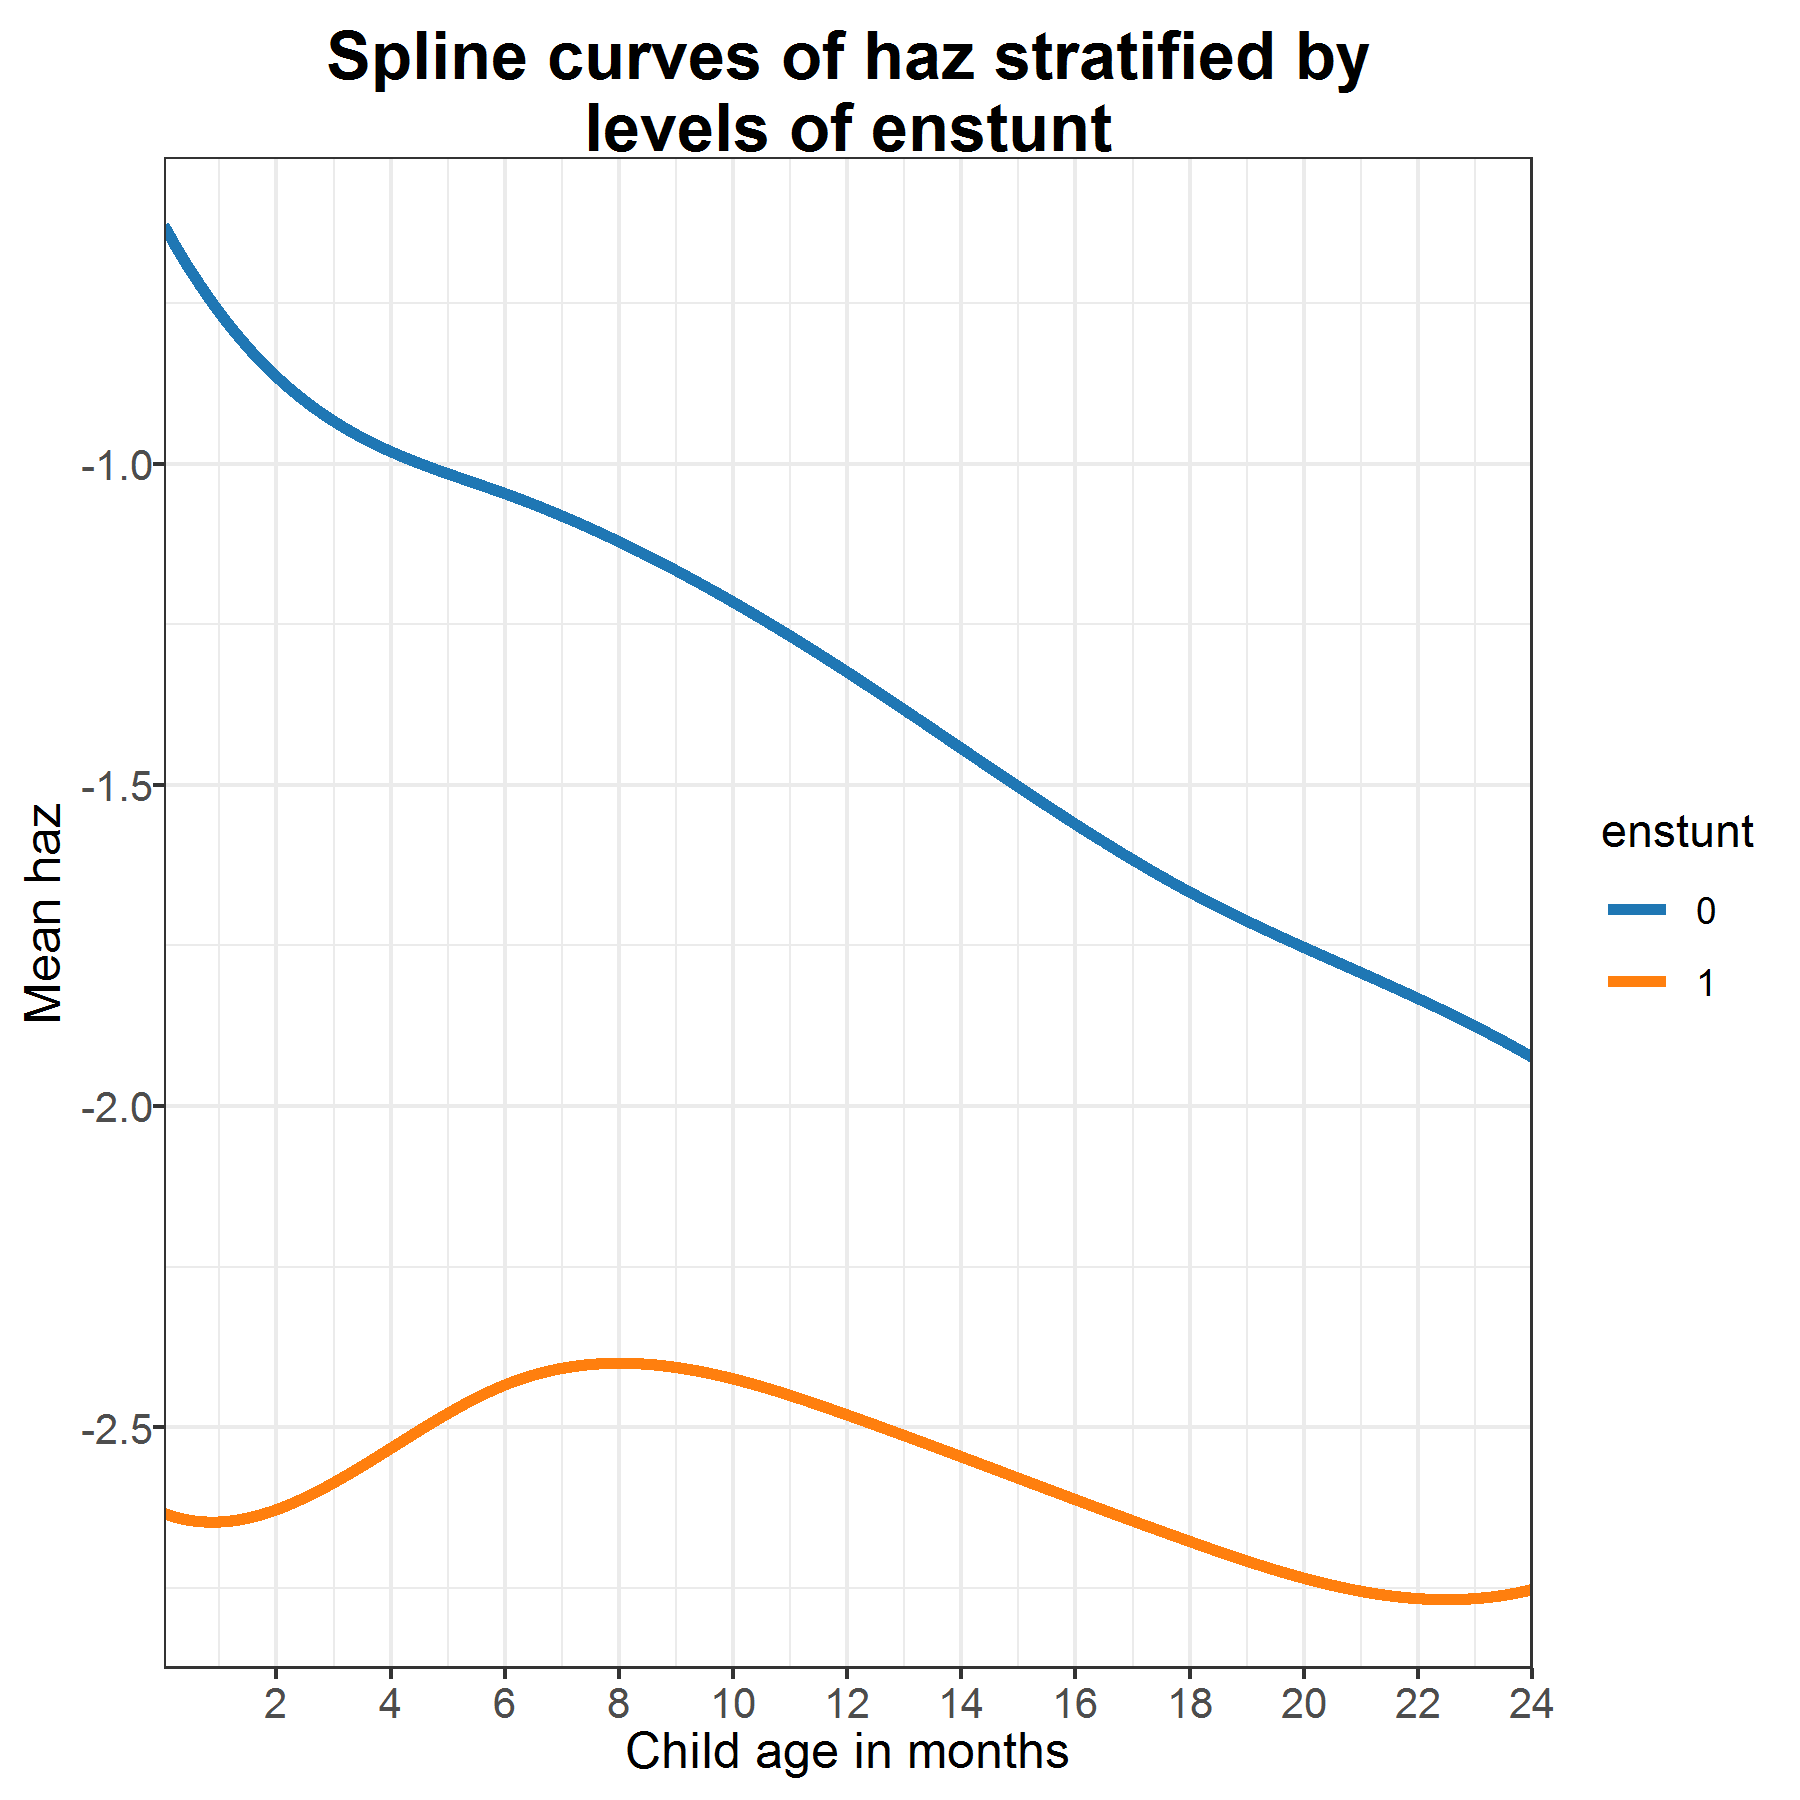
\includegraphics[width=25in]{C:/Users/andre/Documents/HBGDki/causes/ki-longitudinal-manuscripts/figures/risk-factor/spline-plots/haz-enstunt-spline}
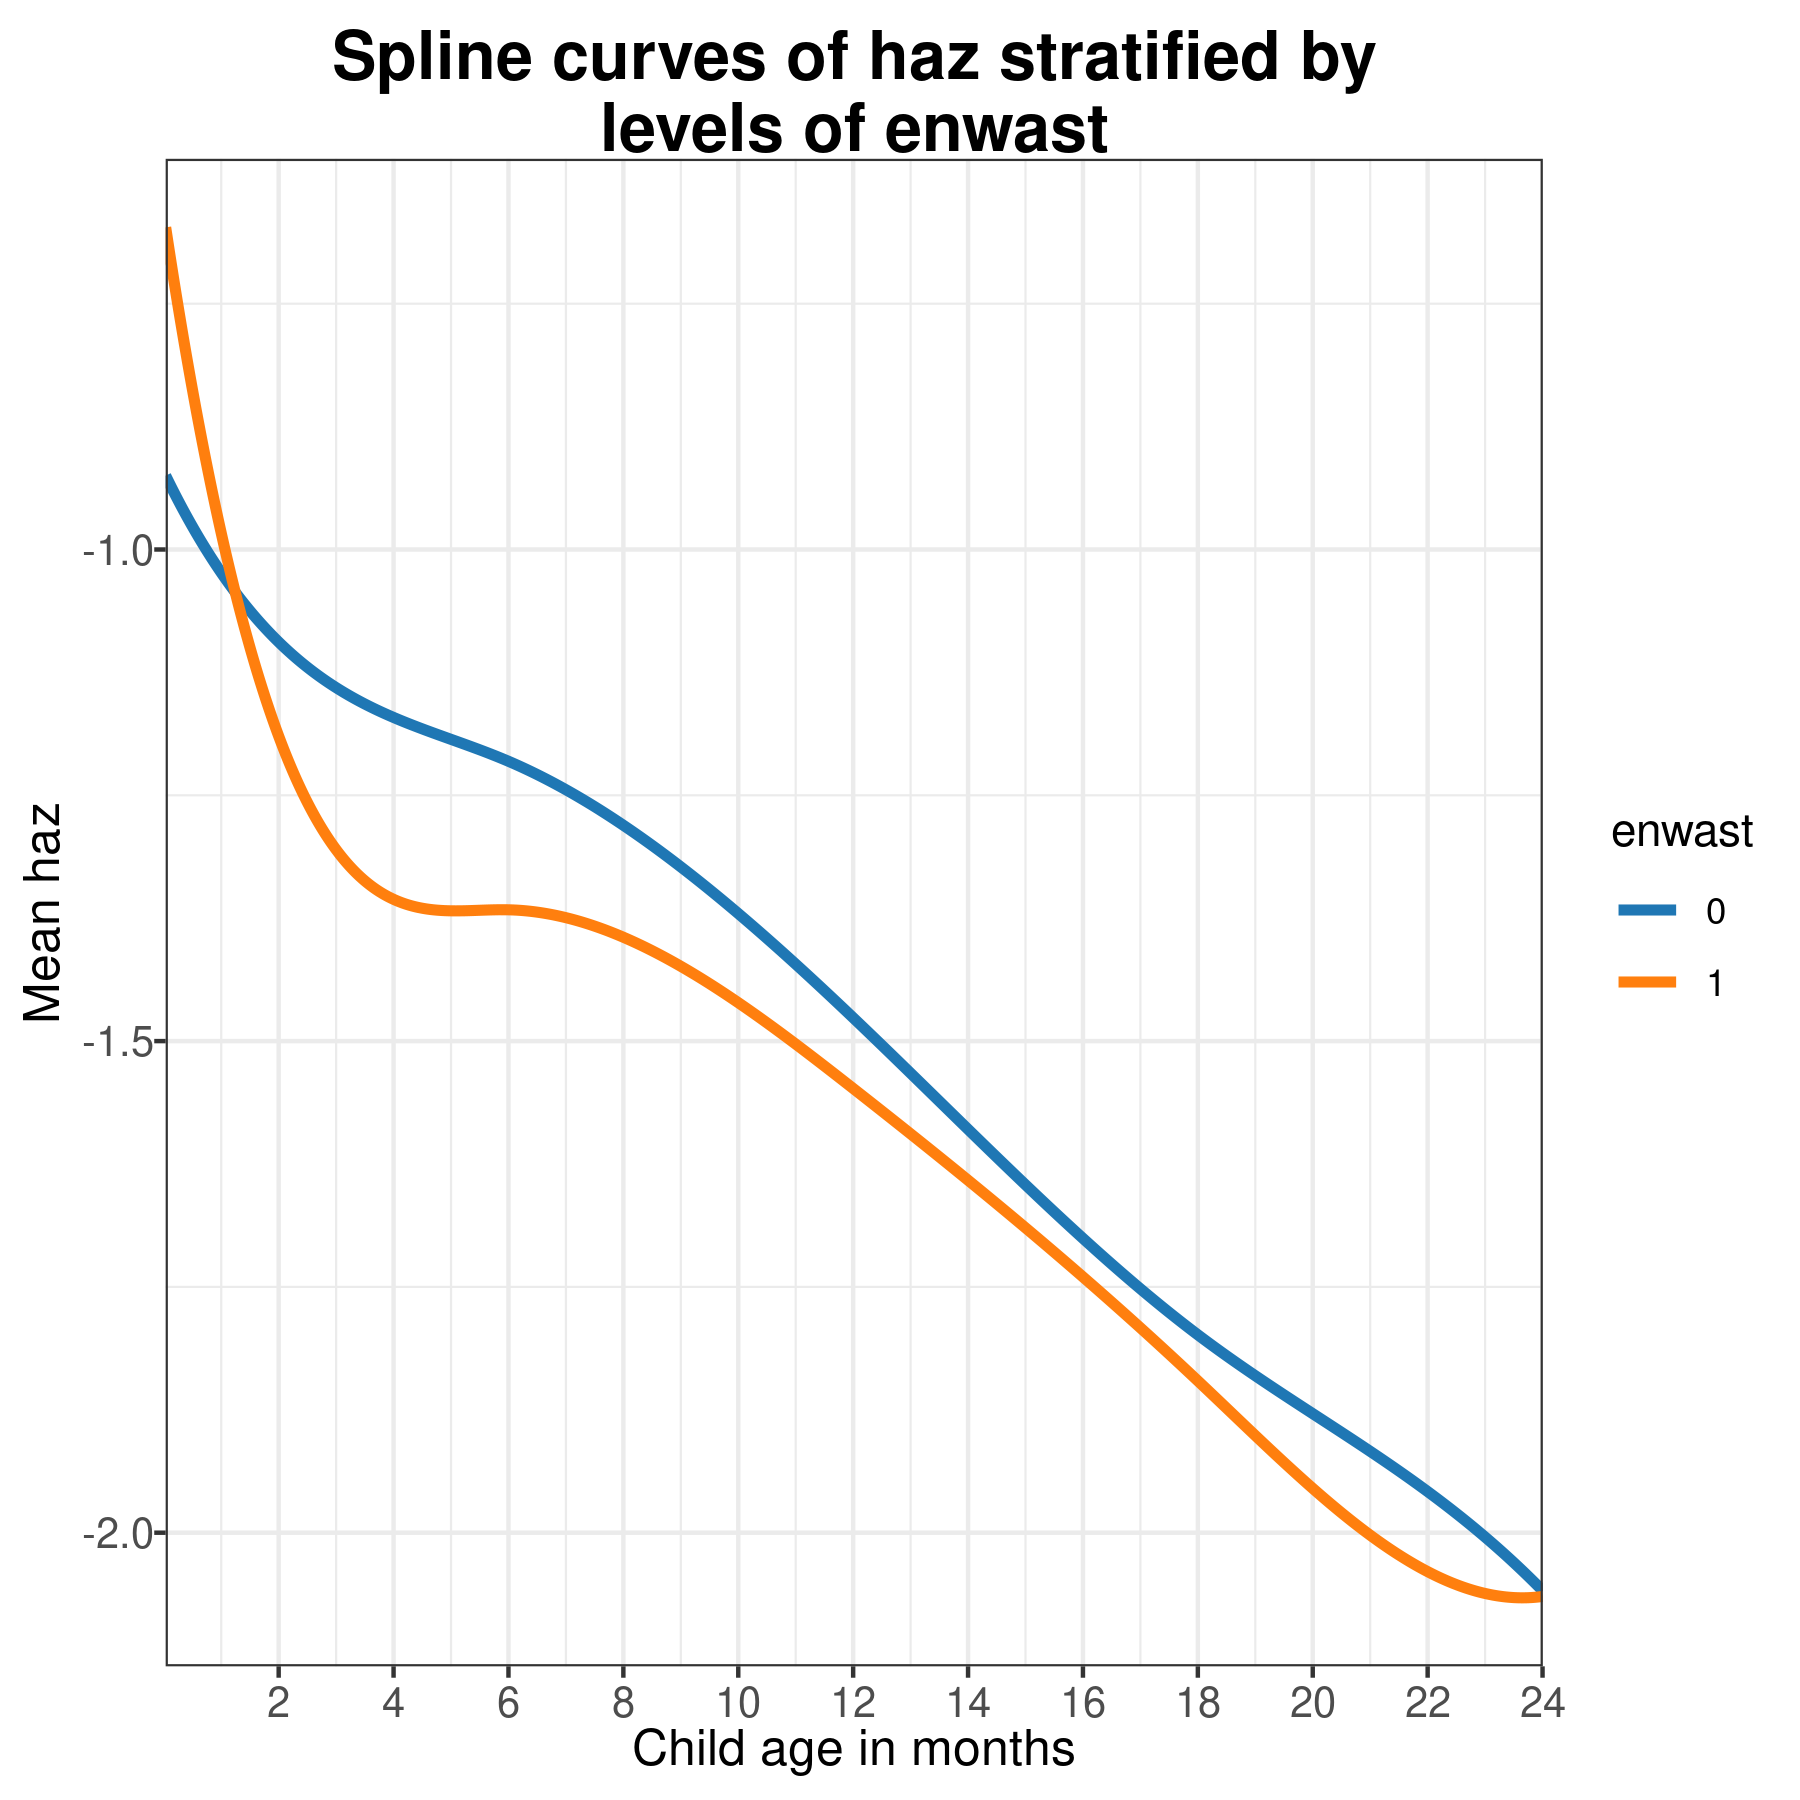
\includegraphics[width=25in]{C:/Users/andre/Documents/HBGDki/causes/ki-longitudinal-manuscripts/figures/risk-factor/spline-plots/haz-enwast-spline}
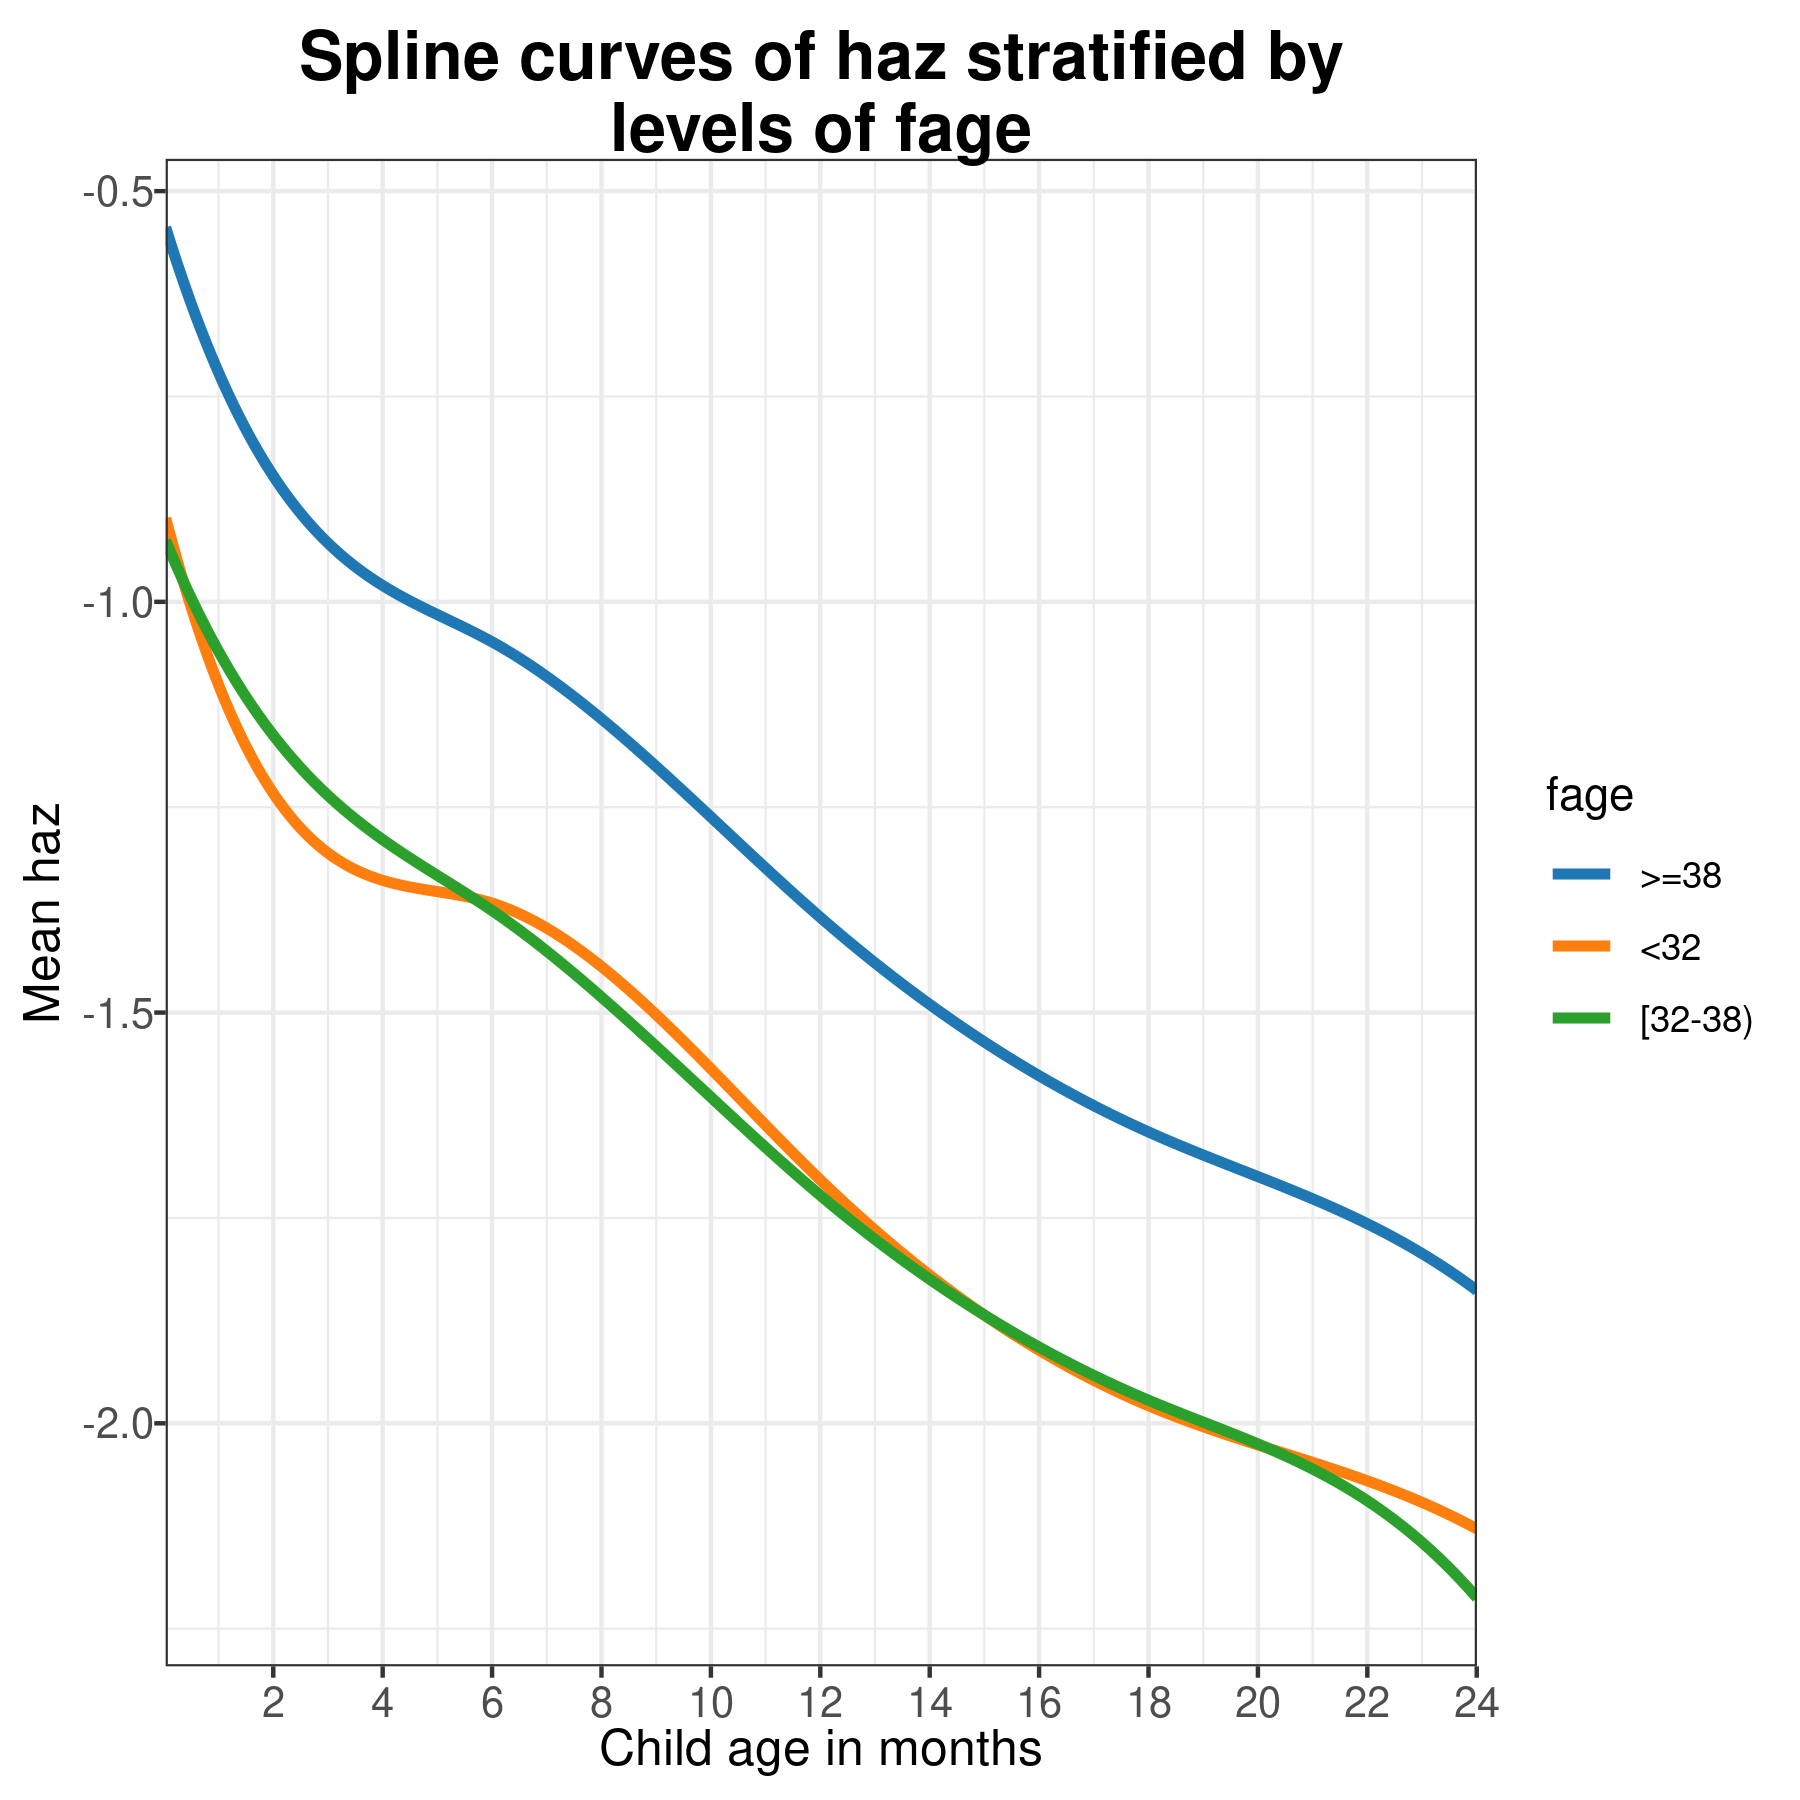
\includegraphics[width=25in]{C:/Users/andre/Documents/HBGDki/causes/ki-longitudinal-manuscripts/figures/risk-factor/spline-plots/haz-fage-spline}
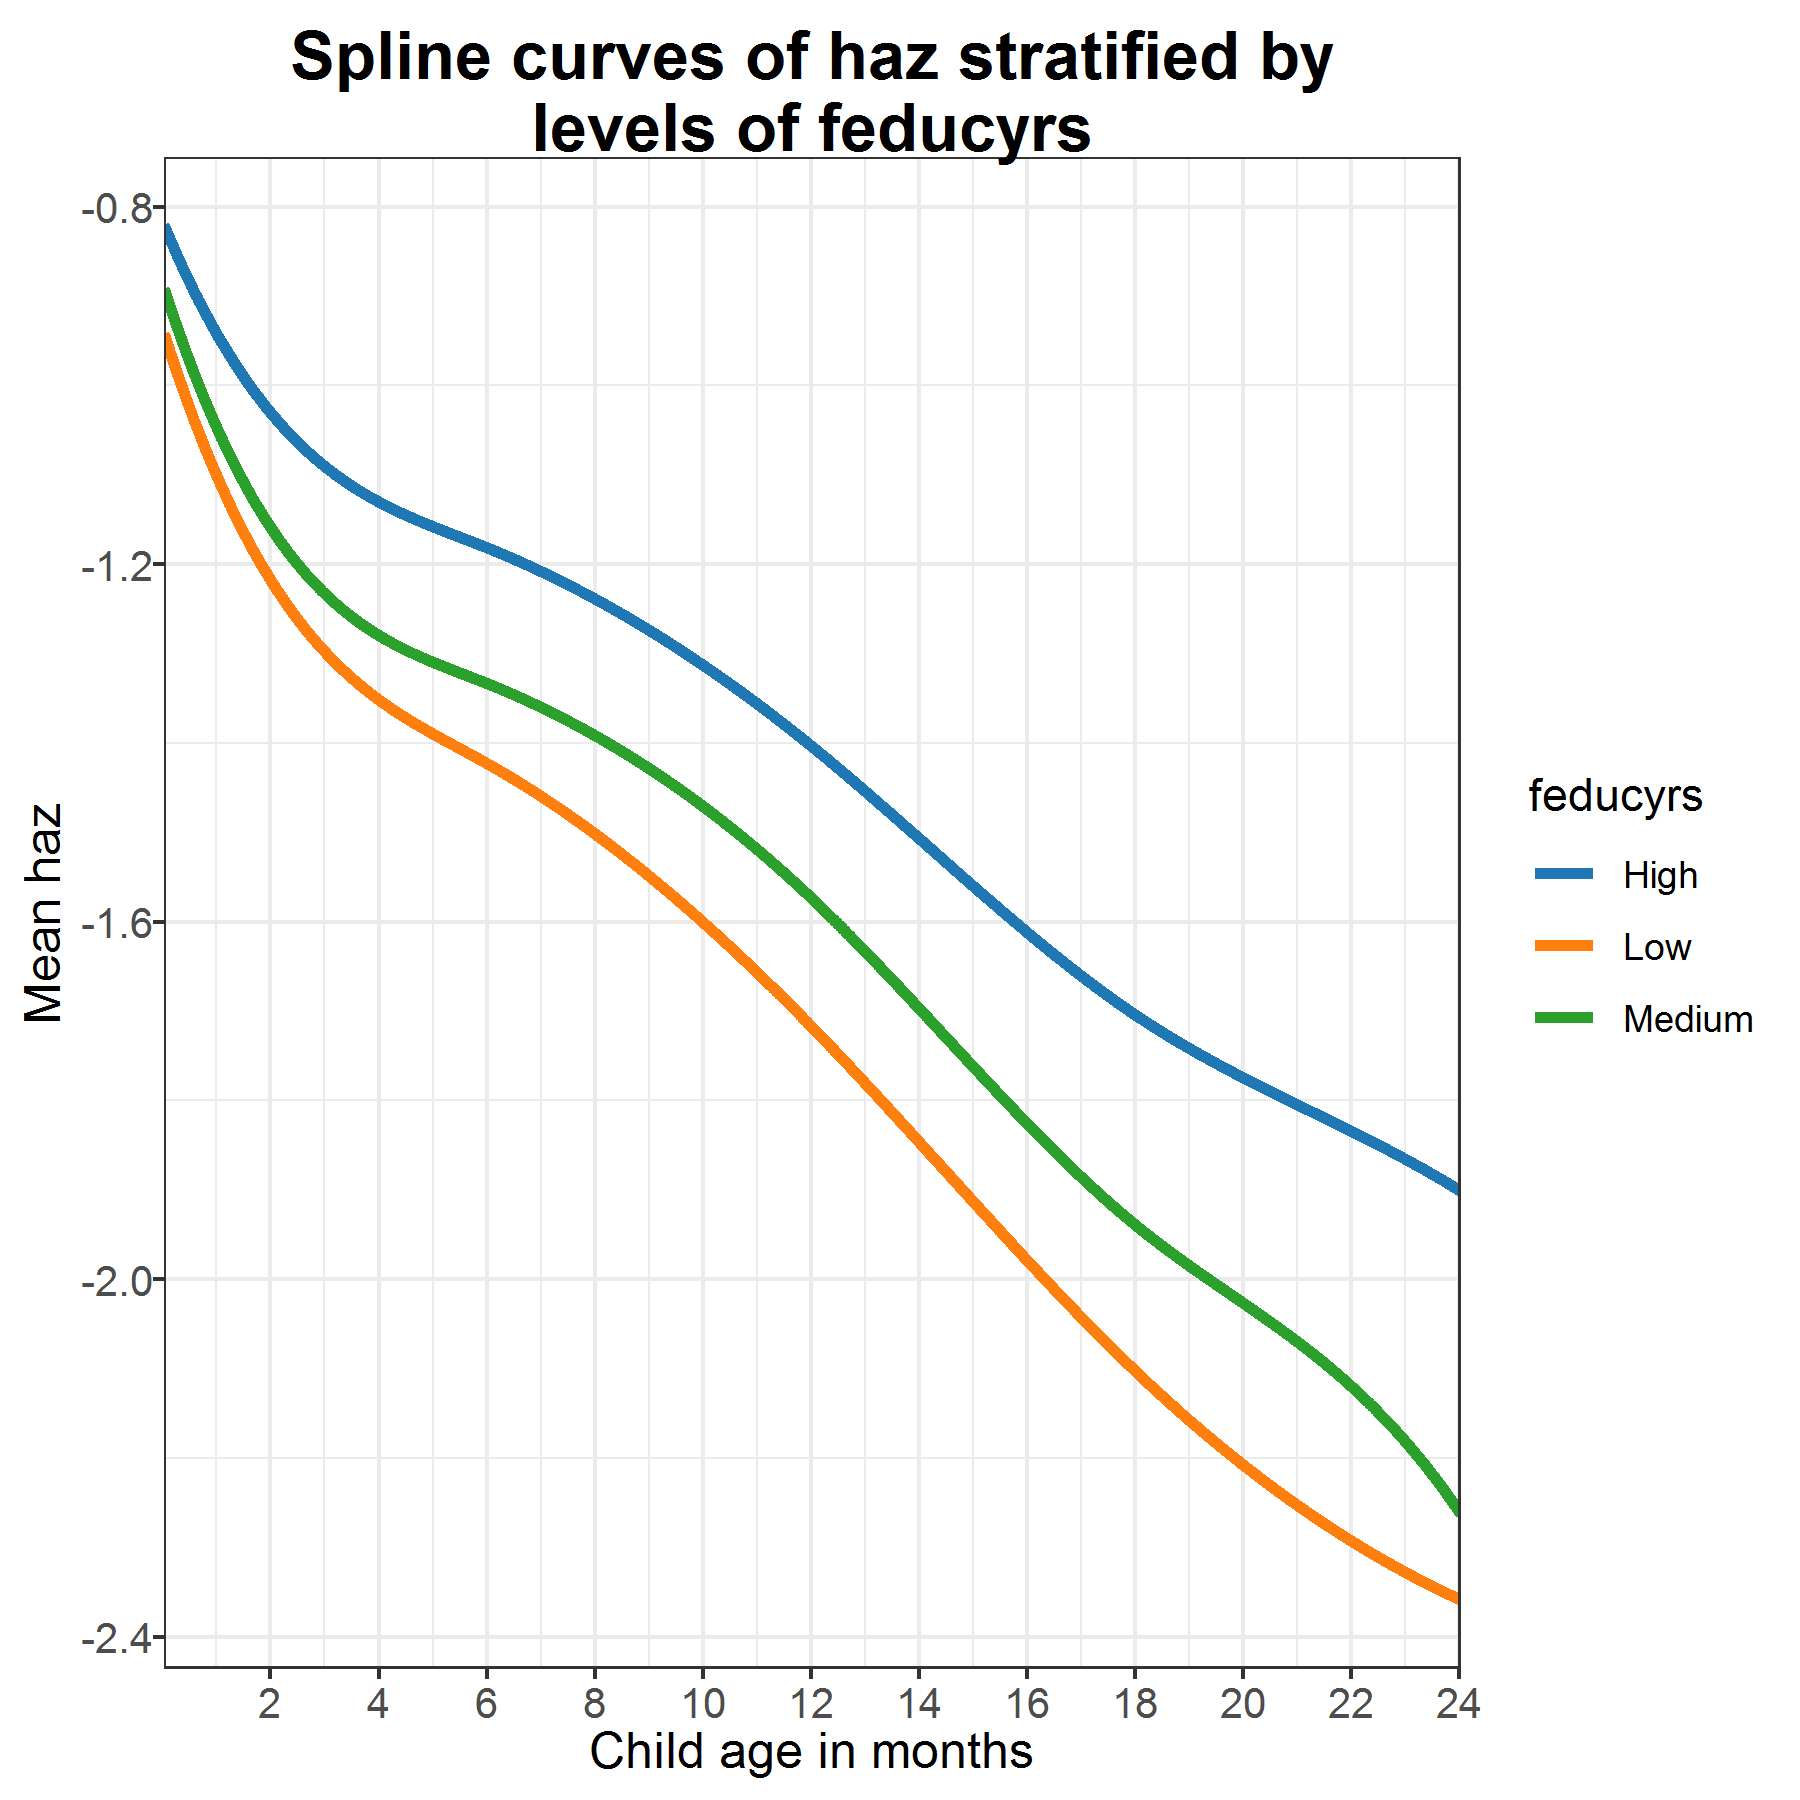
\includegraphics[width=25in]{C:/Users/andre/Documents/HBGDki/causes/ki-longitudinal-manuscripts/figures/risk-factor/spline-plots/haz-feducyrs-spline}
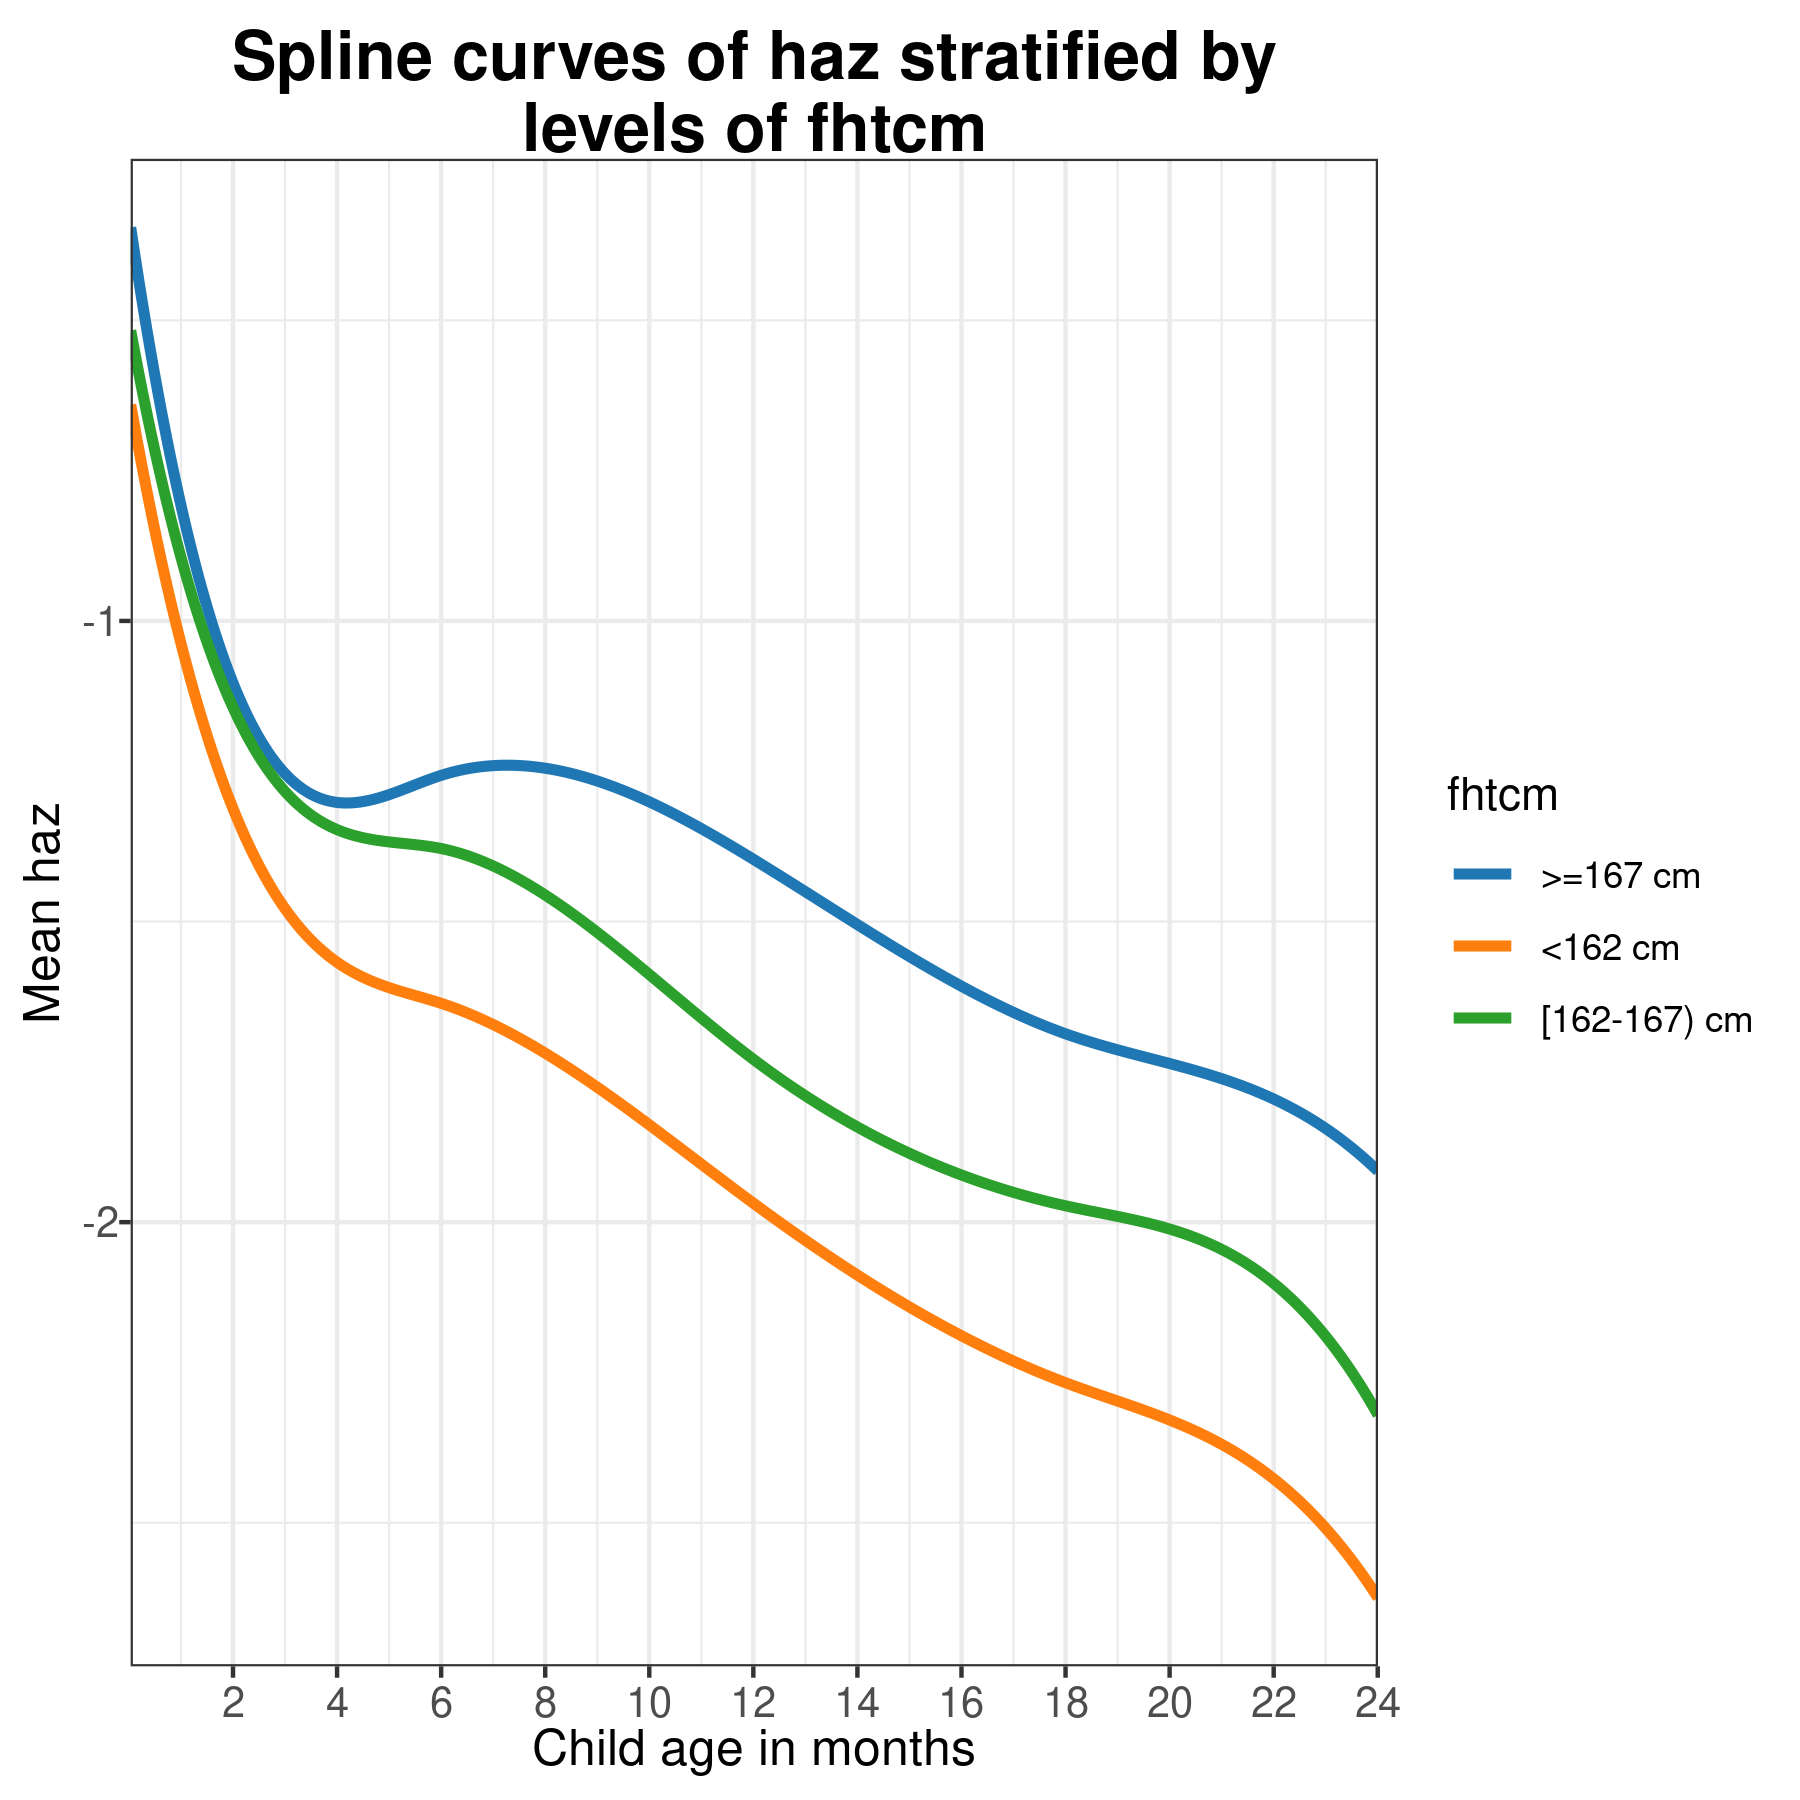
\includegraphics[width=25in]{C:/Users/andre/Documents/HBGDki/causes/ki-longitudinal-manuscripts/figures/risk-factor/spline-plots/haz-fhtcm-spline}
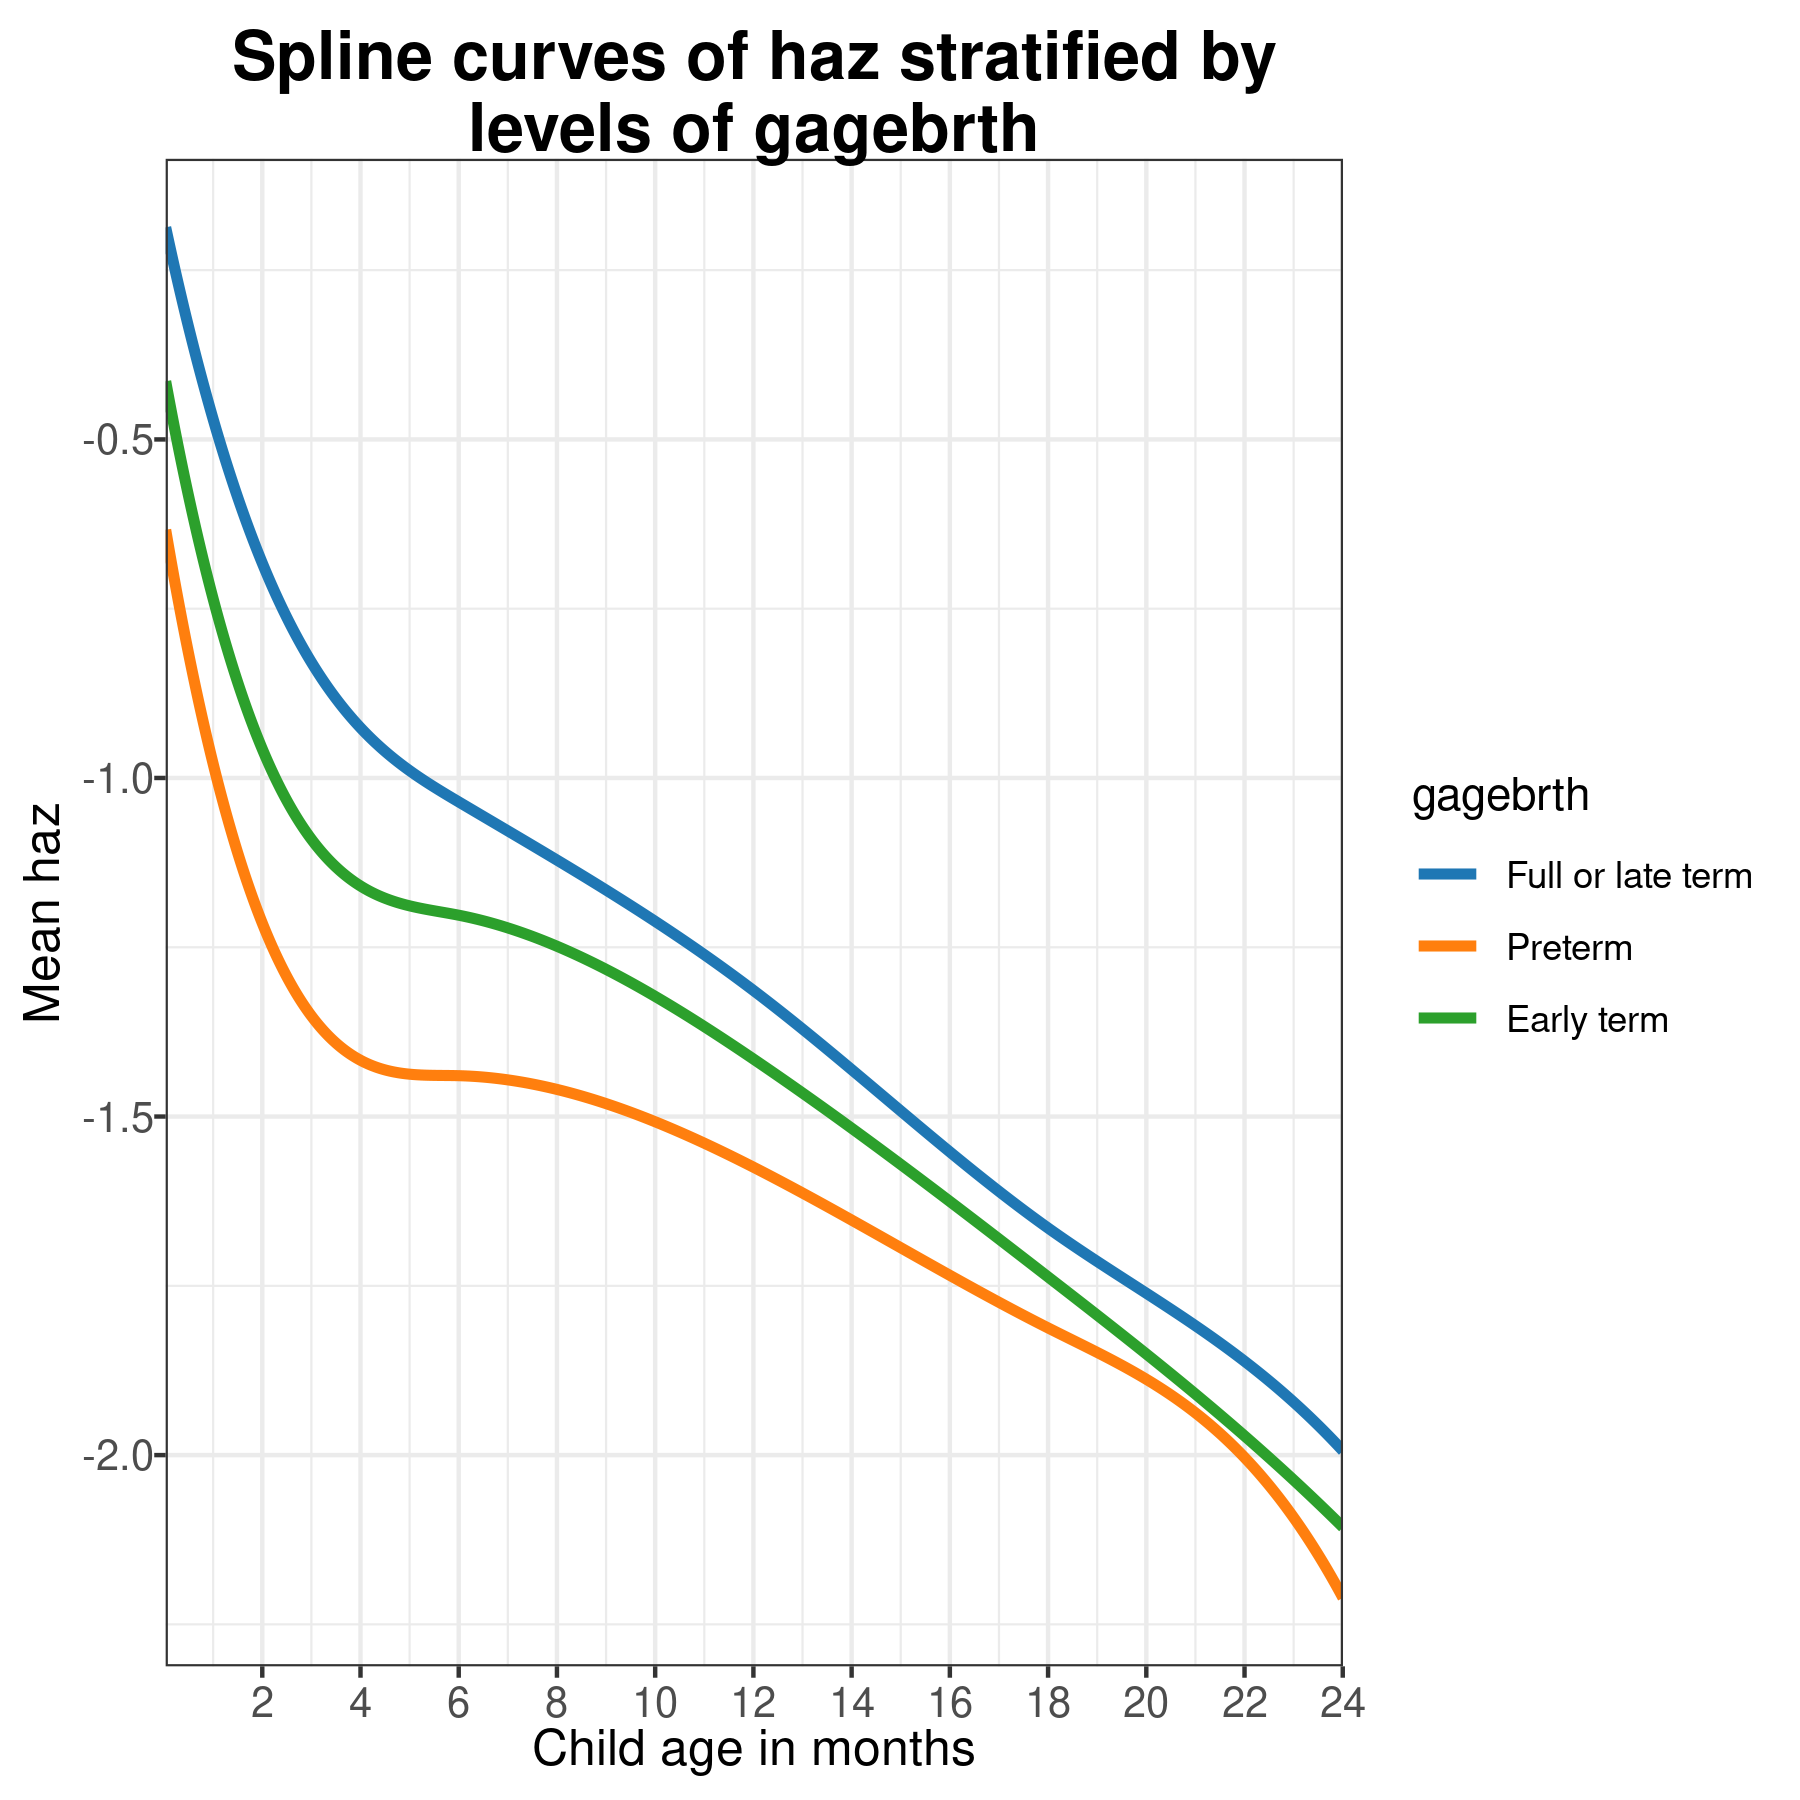
\includegraphics[width=25in]{C:/Users/andre/Documents/HBGDki/causes/ki-longitudinal-manuscripts/figures/risk-factor/spline-plots/haz-gagebrth-spline}
\includegraphics[width=25in]{C:/Users/andre/Documents/HBGDki/causes/ki-longitudinal-manuscripts/figures/risk-factor/spline-plots/haz-hdlvry-spline}
\includegraphics[width=25in]{C:/Users/andre/Documents/HBGDki/causes/ki-longitudinal-manuscripts/figures/risk-factor/spline-plots/haz-hfoodsec-spline}
\includegraphics[width=25in]{C:/Users/andre/Documents/HBGDki/causes/ki-longitudinal-manuscripts/figures/risk-factor/spline-plots/haz-hhwealth_quart-spline}
\includegraphics[width=25in]{C:/Users/andre/Documents/HBGDki/causes/ki-longitudinal-manuscripts/figures/risk-factor/spline-plots/haz-impfloor-spline}
\includegraphics[width=25in]{C:/Users/andre/Documents/HBGDki/causes/ki-longitudinal-manuscripts/figures/risk-factor/spline-plots/haz-impsan-spline}
\includegraphics[width=25in]{C:/Users/andre/Documents/HBGDki/causes/ki-longitudinal-manuscripts/figures/risk-factor/spline-plots/haz-mage-spline}
\includegraphics[width=25in]{C:/Users/andre/Documents/HBGDki/causes/ki-longitudinal-manuscripts/figures/risk-factor/spline-plots/haz-meducyrs-spline}
\includegraphics[width=25in]{C:/Users/andre/Documents/HBGDki/causes/ki-longitudinal-manuscripts/figures/risk-factor/spline-plots/haz-nchldlt5-spline}
\includegraphics[width=25in]{C:/Users/andre/Documents/HBGDki/causes/ki-longitudinal-manuscripts/figures/risk-factor/spline-plots/haz-nhh-spline}
\includegraphics[width=25in]{C:/Users/andre/Documents/HBGDki/causes/ki-longitudinal-manuscripts/figures/risk-factor/spline-plots/haz-nrooms-spline}
\includegraphics[width=25in]{C:/Users/andre/Documents/HBGDki/causes/ki-longitudinal-manuscripts/figures/risk-factor/spline-plots/haz-parity-spline}
\includegraphics[width=25in]{C:/Users/andre/Documents/HBGDki/causes/ki-longitudinal-manuscripts/figures/risk-factor/spline-plots/haz-perdiar6-spline}
\includegraphics[width=25in]{C:/Users/andre/Documents/HBGDki/causes/ki-longitudinal-manuscripts/figures/risk-factor/spline-plots/haz-perdiar24-spline}
\includegraphics[width=25in]{C:/Users/andre/Documents/HBGDki/causes/ki-longitudinal-manuscripts/figures/risk-factor/spline-plots/haz-pers_wast-spline}
\includegraphics[width=25in]{C:/Users/andre/Documents/HBGDki/causes/ki-longitudinal-manuscripts/figures/risk-factor/spline-plots/haz-predexfd6-spline}
\includegraphics[width=25in]{C:/Users/andre/Documents/HBGDki/causes/ki-longitudinal-manuscripts/figures/risk-factor/spline-plots/haz-safeh20-spline}
\includegraphics[width=25in]{C:/Users/andre/Documents/HBGDki/causes/ki-longitudinal-manuscripts/figures/risk-factor/spline-plots/haz-sex-spline}
\includegraphics[width=25in]{C:/Users/andre/Documents/HBGDki/causes/ki-longitudinal-manuscripts/figures/risk-factor/spline-plots/haz-single-spline}
\includegraphics[width=25in]{C:/Users/andre/Documents/HBGDki/causes/ki-longitudinal-manuscripts/figures/risk-factor/spline-plots/haz-trth2o-spline}
\includegraphics[width=25in]{C:/Users/andre/Documents/HBGDki/causes/ki-longitudinal-manuscripts/figures/risk-factor/spline-plots/haz-vagbrth-spline}

\hypertarget{secondary-spline-figures---wlz-stratified-by-levels-of-exposures}{%
\subsection{Secondary spline figures - WLZ stratified by levels of exposures}\label{secondary-spline-figures---wlz-stratified-by-levels-of-exposures}}

\includegraphics[width=25in]{C:/Users/andre/Documents/HBGDki/causes/ki-longitudinal-manuscripts/figures/risk-factor/spline-plots/whz-birthlen-spline}
\includegraphics[width=25in]{C:/Users/andre/Documents/HBGDki/causes/ki-longitudinal-manuscripts/figures/risk-factor/spline-plots/whz-birthwt-spline}
\includegraphics[width=25in]{C:/Users/andre/Documents/HBGDki/causes/ki-longitudinal-manuscripts/figures/risk-factor/spline-plots/whz-cleanck-spline}
\includegraphics[width=25in]{C:/Users/andre/Documents/HBGDki/causes/ki-longitudinal-manuscripts/figures/risk-factor/spline-plots/whz-earlybf-spline}
\includegraphics[width=25in]{C:/Users/andre/Documents/HBGDki/causes/ki-longitudinal-manuscripts/figures/risk-factor/spline-plots/whz-enstunt-spline}
\includegraphics[width=25in]{C:/Users/andre/Documents/HBGDki/causes/ki-longitudinal-manuscripts/figures/risk-factor/spline-plots/whz-enwast-spline}
\includegraphics[width=25in]{C:/Users/andre/Documents/HBGDki/causes/ki-longitudinal-manuscripts/figures/risk-factor/spline-plots/whz-fage-spline}
\includegraphics[width=25in]{C:/Users/andre/Documents/HBGDki/causes/ki-longitudinal-manuscripts/figures/risk-factor/spline-plots/whz-feducyrs-spline}
\includegraphics[width=25in]{C:/Users/andre/Documents/HBGDki/causes/ki-longitudinal-manuscripts/figures/risk-factor/spline-plots/whz-fhtcm-spline}
\includegraphics[width=25in]{C:/Users/andre/Documents/HBGDki/causes/ki-longitudinal-manuscripts/figures/risk-factor/spline-plots/whz-gagebrth-spline}
\includegraphics[width=25in]{C:/Users/andre/Documents/HBGDki/causes/ki-longitudinal-manuscripts/figures/risk-factor/spline-plots/whz-hdlvry-spline}
\includegraphics[width=25in]{C:/Users/andre/Documents/HBGDki/causes/ki-longitudinal-manuscripts/figures/risk-factor/spline-plots/whz-hfoodsec-spline}
\includegraphics[width=25in]{C:/Users/andre/Documents/HBGDki/causes/ki-longitudinal-manuscripts/figures/risk-factor/spline-plots/whz-hhwealth_quart-spline}
\includegraphics[width=25in]{C:/Users/andre/Documents/HBGDki/causes/ki-longitudinal-manuscripts/figures/risk-factor/spline-plots/whz-impfloor-spline}
\includegraphics[width=25in]{C:/Users/andre/Documents/HBGDki/causes/ki-longitudinal-manuscripts/figures/risk-factor/spline-plots/whz-impsan-spline}
\includegraphics[width=25in]{C:/Users/andre/Documents/HBGDki/causes/ki-longitudinal-manuscripts/figures/risk-factor/spline-plots/whz-mage-spline}
\includegraphics[width=25in]{C:/Users/andre/Documents/HBGDki/causes/ki-longitudinal-manuscripts/figures/risk-factor/spline-plots/whz-meducyrs-spline}
\includegraphics[width=25in]{C:/Users/andre/Documents/HBGDki/causes/ki-longitudinal-manuscripts/figures/risk-factor/spline-plots/whz-nchldlt5-spline}
\includegraphics[width=25in]{C:/Users/andre/Documents/HBGDki/causes/ki-longitudinal-manuscripts/figures/risk-factor/spline-plots/whz-nhh-spline}
\includegraphics[width=25in]{C:/Users/andre/Documents/HBGDki/causes/ki-longitudinal-manuscripts/figures/risk-factor/spline-plots/whz-nrooms-spline}
\includegraphics[width=25in]{C:/Users/andre/Documents/HBGDki/causes/ki-longitudinal-manuscripts/figures/risk-factor/spline-plots/whz-parity-spline}
\includegraphics[width=25in]{C:/Users/andre/Documents/HBGDki/causes/ki-longitudinal-manuscripts/figures/risk-factor/spline-plots/whz-perdiar6-spline}
\includegraphics[width=25in]{C:/Users/andre/Documents/HBGDki/causes/ki-longitudinal-manuscripts/figures/risk-factor/spline-plots/whz-perdiar24-spline}
\includegraphics[width=25in]{C:/Users/andre/Documents/HBGDki/causes/ki-longitudinal-manuscripts/figures/risk-factor/spline-plots/whz-pers_wast-spline}
\includegraphics[width=25in]{C:/Users/andre/Documents/HBGDki/causes/ki-longitudinal-manuscripts/figures/risk-factor/spline-plots/whz-predexfd6-spline}
\includegraphics[width=25in]{C:/Users/andre/Documents/HBGDki/causes/ki-longitudinal-manuscripts/figures/risk-factor/spline-plots/whz-safeh20-spline}
\includegraphics[width=25in]{C:/Users/andre/Documents/HBGDki/causes/ki-longitudinal-manuscripts/figures/risk-factor/spline-plots/whz-sex-spline}
\includegraphics[width=25in]{C:/Users/andre/Documents/HBGDki/causes/ki-longitudinal-manuscripts/figures/risk-factor/spline-plots/whz-single-spline}
\includegraphics[width=25in]{C:/Users/andre/Documents/HBGDki/causes/ki-longitudinal-manuscripts/figures/risk-factor/spline-plots/whz-trth2o-spline}
\includegraphics[width=25in]{C:/Users/andre/Documents/HBGDki/causes/ki-longitudinal-manuscripts/figures/risk-factor/spline-plots/whz-vagbrth-spline}

\hypertarget{heatmaps}{%
\chapter{Heatmaps}\label{heatmaps}}

\raggedright

The heatmaps below are of the same design as Extended Data Figure 2, and show the significance and direction of estimates through the cell colors, separated across primary outcomes by child age. Red and orange cells are harmful exposures, while blue and green cells are protective exposures. The outcomes are labeled at the top of the columns, with each set of three columns the set of three ages analyzed for that outcome. Each row is a level of an exposure variable, with reference levels excluded. Rows are sorted top to bottom by increasing average p-value. Grey cells denote comparisons that were not estimated or could not be estimated because of data sparsity in the exposure-outcome combination. The first plot included region-stratified estimates, the second shows significance of estimates pooled across cohorts using fixed effects models, and the third shows significance of unadjusted estimates.

\hypertarget{heatmap-of-significance-of-estimates-region-stratified}{%
\section{Heatmap of significance of estimates, region stratified}\label{heatmap-of-significance-of-estimates-region-stratified}}

\includegraphics[width=58.33in]{C:/Users/andre/Documents/HBGDki/causes/ki-longitudinal-manuscripts/figures/risk-factor/fig-sig-heatmap_regionstrat}

\hypertarget{heatmap-of-significance-of-estimates-pooled-using-fixed-effects}{%
\section{Heatmap of significance of estimates pooled using fixed effects}\label{heatmap-of-significance-of-estimates-pooled-using-fixed-effects}}

\includegraphics[width=47.92in]{C:/Users/andre/Documents/HBGDki/causes/ki-longitudinal-manuscripts/figures/risk-factor/fig-sig-heatmap_FE}

\hypertarget{heatmap-of-significance-of-estimate-unadjusted}{%
\section{Heatmap of significance of estimate, unadjusted}\label{heatmap-of-significance-of-estimate-unadjusted}}

\includegraphics[width=47.92in]{C:/Users/andre/Documents/HBGDki/causes/ki-longitudinal-manuscripts/figures/risk-factor/fig-sig-heatmap_unadj}

\hypertarget{mortality}{%
\chapter{Mortality Sensitivity Analyses}\label{mortality}}

\raggedright

\hypertarget{comparisons-of-associations-between-early-growth-failure-and-different-ages-of-mortality}{%
\subsection{Comparisons of associations between early growth failure and different ages of mortality}\label{comparisons-of-associations-between-early-growth-failure-and-different-ages-of-mortality}}

\includegraphics[width=21.67in]{C:/Users/andre/Documents/HBGDki/causes/ki-longitudinal-manuscripts/figures/risk-factor/fig-mort-RR}

\hypertarget{comparisons-of-associations-between-early-growth-failure-and-different-ages-of-mortality-pooled-using-fixed-effects}{%
\subsection{Comparisons of associations between early growth failure and different ages of mortality, pooled using fixed effects}\label{comparisons-of-associations-between-early-growth-failure-and-different-ages-of-mortality-pooled-using-fixed-effects}}

\includegraphics[width=21.67in]{C:/Users/andre/Documents/HBGDki/causes/ki-longitudinal-manuscripts/figures/risk-factor/fig-mort-RR-time-death_FE}

\hypertarget{comparisons-of-associations-between-early-growth-failure-and-different-ages-of-mortality-dropping-biyearly-measured-cohorts}{%
\subsection{Comparisons of associations between early growth failure and different ages of mortality, dropping biyearly-measured cohorts}\label{comparisons-of-associations-between-early-growth-failure-and-different-ages-of-mortality-dropping-biyearly-measured-cohorts}}

\includegraphics[width=21.67in]{C:/Users/andre/Documents/HBGDki/causes/ki-longitudinal-manuscripts/figures/risk-factor/fig-mort-RR-sens}

\hypertarget{comparisons-of-associations-between-early-growth-failure-and-mortality-and-serious-growth-failure-stratified-by-region}{%
\subsection{Comparisons of associations between early growth failure and mortality and serious growth failure, stratified by region}\label{comparisons-of-associations-between-early-growth-failure-and-mortality-and-serious-growth-failure-stratified-by-region}}

\includegraphics[width=66.67in]{C:/Users/andre/Documents/HBGDki/causes/ki-longitudinal-manuscripts/figures/risk-factor/fig-mort-morb-RR_Region}

\hypertarget{comparisons-of-associations-between-early-growth-failure-and-mortality-and-serious-growth-failure-pooled-using-fixed-effects}{%
\subsection{Comparisons of associations between early growth failure and mortality and serious growth failure, pooled using fixed effects}\label{comparisons-of-associations-between-early-growth-failure-and-mortality-and-serious-growth-failure-pooled-using-fixed-effects}}

\includegraphics[width=58.33in]{C:/Users/andre/Documents/HBGDki/causes/ki-longitudinal-manuscripts/figures/risk-factor/fig-mort-morb-RR_FE}

\hypertarget{no-PROBIT}{%
\chapter{Sensitivity to dropping PROBIT trial}\label{no-PROBIT}}

\raggedright

\hypertarget{comparison-of-attributable-differences-estimated-with-and-without-the-probit-trial}{%
\section{Comparison of attributable differences estimated with and without the PROBIT trial}\label{comparison-of-attributable-differences-estimated-with-and-without-the-probit-trial}}

Because PROBIT was the only European study, we also conducted a sensitivity analysis as to the effect of removing PROBIT on attributable differences at 24 months (within the exposures measures during the PROBIT trial). Other than for the estimated associations between father's height and child Z-scores at 24 months (which was measured in few other studies), PROBIT is not highly influential.

\includegraphics[width=66.67in]{C:/Users/andre/Documents/HBGDki/causes/ki-longitudinal-manuscripts/figures/risk-factor/fig-PAR-Probit-sensitivity}

\hypertarget{RR-forest}{%
\chapter{Forest plots of relative risk}\label{RR-forest}}

\raggedright

\hypertarget{outcome-ever_co-exposure-sex-age-0-24-months}{%
\subsubsection{Outcome: ever\_co Exposure: sex Age: 0-24 months}\label{outcome-ever_co-exposure-sex-age-0-24-months}}

  \bibliography{book.bib,packages.bib}

\end{document}
